%&preformat-disser
\RequirePackage[l2tabu,orthodox]{nag} % Раскомментировав, можно в логе получать рекомендации относительно правильного использования пакетов и предупреждения об устаревших и нерекомендуемых пакетах
% Формат А4, 14pt (ГОСТ Р 7.0.11-2011, 5.3.6)
\documentclass[a4paper,14pt,oneside,openany]{memoir}

%%%%%%%%%%%%%%%%%%%%%%%%%%%%%%%%%%%%%%%%%%%%%%%%%%%%%%%
%%%% Файл упрощённых настроек шаблона автореферата %%%%
%%%%%%%%%%%%%%%%%%%%%%%%%%%%%%%%%%%%%%%%%%%%%%%%%%%%%%%

%%% Инициализирование переменных, не трогать!  %%%
\newcounter{showperssign}
\newcounter{showsecrsign}
\newcounter{showopplead}
%%%%%%%%%%%%%%%%%%%%%%%%%%%%%%%%%%%%%%%%%%%%%%%%%%%%%%%

%%% Список публикаций %%%
\makeatletter
\@ifundefined{c@usefootcite}{
  \newcounter{usefootcite}
  \setcounter{usefootcite}{0} % 0 --- два списка литературы;
                              % 1 --- список публикаций автора + цитирование
                              %       других работ в сносках
}{}
\makeatother

\makeatletter
\@ifundefined{c@bibgrouped}{
  \newcounter{bibgrouped}
  \setcounter{bibgrouped}{0}  % 0 --- единый список работ автора;
                              % 1 --- сгруппированные работы автора
}{}
\makeatother

%%% Область упрощённого управления оформлением %%%

%% Управление зазором между подрисуночной подписью и основным текстом %%
\setlength{\belowcaptionskip}{10pt plus 20pt minus 2pt}


%% Подпись таблиц %%

% смещение строк подписи после первой
\newcommand{\tabindent}{0cm}

% тип форматирования таблицы
% plain --- название и текст в одной строке
% split --- название и текст в разных строках
\newcommand{\tabformat}{plain}

%%% настройки форматирования таблицы `plain'

% выравнивание по центру подписи, состоящей из одной строки
% true  --- выравнивать
% false --- не выравнивать
\newcommand{\tabsinglecenter}{false}

% выравнивание подписи таблиц
% justified   --- выравнивать как обычный текст
% centering   --- выравнивать по центру
% centerlast  --- выравнивать по центру только последнюю строку
% centerfirst --- выравнивать по центру только первую строку
% raggedleft  --- выравнивать по правому краю
% raggedright --- выравнивать по левому краю
\newcommand{\tabjust}{justified}

% Разделитель записи «Таблица #» и названия таблицы
\newcommand{\tablabelsep}{~\cyrdash\ }

%%% настройки форматирования таблицы `split'

% положение названия таблицы
% \centering   --- выравнивать по центру
% \raggedleft  --- выравнивать по правому краю
% \raggedright --- выравнивать по левому краю
\newcommand{\splitformatlabel}{\raggedleft}

% положение текста подписи
% \centering   --- выравнивать по центру
% \raggedleft  --- выравнивать по правому краю
% \raggedright --- выравнивать по левому краю
\newcommand{\splitformattext}{\raggedright}

%% Подпись рисунков %%
%Разделитель записи «Рисунок #» и названия рисунка
\newcommand{\figlabelsep}{~\cyrdash\ }  % (ГОСТ 2.105, 4.3.1)
                                        % "--- здесь не работает

%Демонстрация подписи диссертанта на автореферате
\setcounter{showperssign}{1}  % 0 --- не показывать;
                              % 1 --- показывать
%Демонстрация подписи учёного секретаря на автореферате
\setcounter{showsecrsign}{1}  % 0 --- не показывать;
                              % 1 --- показывать
%Демонстрация информации об оппонентах и ведущей организации на автореферате
\setcounter{showopplead}{1}   % 0 --- не показывать;
                              % 1 --- показывать

%%% Цвета гиперссылок %%%
% Latex color definitions: http://latexcolor.com/
\definecolor{linkcolor}{rgb}{0.9,0,0}
\definecolor{citecolor}{rgb}{0,0.6,0}
\definecolor{urlcolor}{rgb}{0,0,1}
%\definecolor{linkcolor}{rgb}{0,0,0} %black
%\definecolor{citecolor}{rgb}{0,0,0} %black
%\definecolor{urlcolor}{rgb}{0,0,0} %black
            % общие настройки шаблона
%%% Проверка используемого TeX-движка %%%
\newif\ifxetexorluatex   % определяем новый условный оператор (http://tex.stackexchange.com/a/47579)
\ifxetex
    \xetexorluatextrue
\else
    \ifluatex
        \xetexorluatextrue
    \else
        \xetexorluatexfalse
    \fi
\fi

\newif\ifsynopsis           % Условие, проверяющее, что документ --- автореферат

\usepackage{etoolbox}[2015/08/02]   % Для продвинутой проверки разных условий
\providebool{presentation}

\usepackage{comment}    % Позволяет убирать блоки текста (добавляет
                        % окружение comment и команду \excludecomment)

%%% Поля и разметка страницы %%%
\usepackage{pdflscape}  % Для включения альбомных страниц
\usepackage{geometry}   % Для последующего задания полей

%%% Математические пакеты %%%
\usepackage[bb=boondox]{mathalfa}   % 0 и 1
\usepackage{amsthm,amsmath,amscd}   % Математические дополнения от AMS
\usepackage{amsfonts,amssymb}       % Математические дополнения от AMS
\usepackage{mathtools}              % Добавляет окружение multlined
\usepackage{xfrac}                  % Красивые дроби
\usepackage[
    locale = DE,
    list-separator       = {;\,},
    list-final-separator = {;\,},
    list-pair-separator  = {;\,},
    list-units           = single,
    range-units          = single,
    range-phrase={\text{\ensuremath{-}}},
    % quotient-mode        = fraction, % красивые дроби могут не соответствовать ГОСТ
    fraction-function    = \sfrac,
    separate-uncertainty,
    ]{siunitx}                      % Размерности SI
\sisetup{inter-unit-product = \ensuremath{{}\cdot{}}}

% Кириллица в нумерации subequations
% Для правильной работы требуется выполнение сразу после загрузки пакетов
\patchcmd{\subequations}{\def\theequation{\theparentequation\alph{equation}}}
{\def\theequation{\theparentequation\asbuk{equation}}}
{\typeout{subequations patched}}{\typeout{subequations not patched}}

%%%% Установки для размера шрифта 14 pt %%%%
%% Формирование переменных и констант для сравнения (один раз для всех подключаемых файлов)%%
%% должно располагаться до вызова пакета fontspec или polyglossia, потому что они сбивают его работу
\newlength{\curtextsize}
\newlength{\bigtextsize}
\setlength{\bigtextsize}{13.9pt}

\makeatletter
%\show\f@size    % неплохо для отслеживания, но вызывает стопорение процесса,
                 % если документ компилируется без команды  -interaction=nonstopmode
\setlength{\curtextsize}{\f@size pt}
\makeatother

%%% Кодировки и шрифты %%%
\ifxetexorluatex
    \PassOptionsToPackage{no-math}{fontspec}    % https://tex.stackexchange.com/a/26295/104425
    \usepackage{polyglossia}[2014/05/21]        % Поддержка многоязычности
                                        % (fontspec подгружается автоматически)
\else
   %%% Решение проблемы копирования текста в буфер кракозябрами
    \ifnumequal{\value{usealtfont}}{0}{}{
        \input glyphtounicode.tex
        \input glyphtounicode-cmr.tex %from pdfx package
        \pdfgentounicode=1
    }
    \usepackage{cmap}   % Улучшенный поиск русских слов в полученном pdf-файле
    \ifnumequal{\value{usealtfont}}{2}{}{
        \defaulthyphenchar=127  % Если стоит до fontenc, то переносы
                                % не впишутся в выделяемый текст при
                                % копировании его в буфер обмена
    }
    \usepackage{textcomp}
    \usepackage[T1,T2A]{fontenc}                    % Поддержка русских букв
    \ifnumequal{\value{usealtfont}}{1}{% Используется pscyr, при наличии
        \IfFileExists{pscyr.sty}{\usepackage{pscyr}}{}  % Подключение pscyr
    }{}
    \usepackage[utf8]{inputenc}[2014/04/30]         % Кодировка utf8
    \usepackage[english, russian]{babel}[2014/03/24]% Языки: русский, английский
    \makeatletter\AtBeginDocument{\let\@elt\relax}\makeatother % babel 3.40 fix
    \ifnumequal{\value{usealtfont}}{2}{
        % http://dxdy.ru/post1238763.html#p1238763
        \usepackage[scaled=0.960]{XCharter}[2017/12/19] % Подключение русифицированных шрифтов XCharter
        \usepackage[charter, vvarbb, scaled=1.048]{newtxmath}[2017/12/14]
        \ifpresentation
        \else
            \setDisplayskipStretch{-0.078}
        \fi
    }{}
\fi

%%% Оформление абзацев %%%
\providebool{newpoly} % polyglossia with indentfirst setting
\boolfalse{newpoly} % setting our new boolean flag to default false
\ifxetexorluatex
    \makeatletter
    \@ifpackagelater{polyglossia}{2019/11/15}{
        \booltrue{newpoly} % setting our new boolean flag to true
    }{}
    \makeatother
\fi
\ifpresentation
\else
    \indentafterchapter     % Красная строка после заголовков типа chapter
    \ifxetexorluatex
        \ifnewpoly
        \else
            \usepackage{indentfirst}
        \fi
    \else
        \usepackage{indentfirst}
    \fi
\fi


%%% Цвета %%%
\ifpresentation
\else
    \usepackage[dvipsnames, table, hyperref]{xcolor} % Совместимо с tikz
\fi

%%% Таблицы %%%
\usepackage{longtable,ltcaption} % Длинные таблицы
\usepackage{multirow,makecell}   % Улучшенное форматирование таблиц
\usepackage{tabu, tabulary}      % таблицы с автоматически подбирающейся
                                 % шириной столбцов (tabu обязательно
                                 % до hyperref вызывать)
\usepackage{threeparttable}      % автоматический подгон ширины подписи таблицы

%%% Общее форматирование
\usepackage{soulutf8}% Поддержка переносоустойчивых подчёркиваний и зачёркиваний
\usepackage{icomma}  % Запятая в десятичных дробях

%%% Оптимизация расстановки переносов и длины последней строки абзаца
\IfFileExists{impnattypo.sty}{% проверка установленности пакета impnattypo
    \ifluatex
        \ifnumequal{\value{draft}}{1}{% Черновик
            \usepackage[hyphenation, lastparline, nosingleletter, homeoarchy,
            rivers, draft]{impnattypo}
        }{% Чистовик
            \usepackage[hyphenation, lastparline, nosingleletter]{impnattypo}
        }
    \else
        \usepackage[hyphenation, lastparline]{impnattypo}
    \fi
}{}

%% Векторная графика

\usepackage{tikz}                   % Продвинутый пакет векторной графики
\usetikzlibrary{chains}             % Для примера tikz рисунка
\usetikzlibrary{shapes.geometric}   % Для примера tikz рисунка
\usetikzlibrary{shapes.symbols}     % Для примера tikz рисунка
\usetikzlibrary{arrows}             % Для примера tikz рисунка

%%% Гиперссылки %%%
\usepackage{hyperref}[2012/11/06]

%%% Изображения %%%
\usepackage{graphicx}[2014/04/25]   % Подключаем пакет работы с графикой
\usepackage{caption}                % Подписи рисунков и таблиц
\usepackage{subcaption}             % Подписи подрисунков и подтаблиц
\usepackage{pdfpages}               % Добавление внешних pdf файлов

%%% Счётчики %%%
\usepackage[figure,table]{totalcount}   % Счётчик рисунков и таблиц
\usepackage{totcount}   % Пакет создания счётчиков на основе последнего номера
                        % подсчитываемого элемента (может требовать дважды
                        % компилировать документ)
\usepackage{totpages}   % Счётчик страниц, совместимый с hyperref (ссылается
                        % на номер последней страницы). Желательно ставить
                        % последним пакетом в преамбуле

%%% Продвинутое управление групповыми ссылками (пока только формулами) %%%
\ifpresentation
\else
    \usepackage[russian]{cleveref} % cleveref имеет сложности со считыванием
    % языка из babel. Такое решение русификации вывода выбрано вместо
    % определения в documentclass из опасности что-то лишнее передать во все
    % остальные пакеты, включая библиографию.
    \creflabelformat{equation}{#2#1#3} % Формат по умолчанию ставил круглые
    % скобки вокруг каждого номера ссылки, теперь просто номера ссылок без
    % какого-либо дополнительного оформления
    \crefrangelabelformat{equation}{#3#1#4\cyrdash#5#2#6} % Интервалы в русском
    % языке принято делать через тире, если иное не оговорено

    % решение проблемы с "и" в \labelcref
    % https://tex.stackexchange.com/a/455124/104425
    \ifxetexorluatex
        \DeclareTextSymbol{\cyri}\UnicodeEncodingName{"0438} % и
    \fi

    % Добавление возможности использования пробелов в \labelcref
    % https://tex.stackexchange.com/a/340502/104425
    \usepackage{kvsetkeys}
    \makeatletter
    \let\org@@cref\@cref
    \renewcommand*{\@cref}[2]{%
        \edef\process@me{%
            \noexpand\org@@cref{#1}{\zap@space#2 \@empty}%
        }\process@me
    }
    \makeatother

    \newcommand{\eqrefs}[1]{(\labelcref{#1})}
    \newcommand{\refs}[1]{\labelcref{#1}}
\fi

\usepackage{placeins} % для \FloatBarrier

\ifnumequal{\value{draft}}{1}{% Черновик
    \usepackage[firstpage]{draftwatermark}
    \SetWatermarkText{DRAFT}
    \SetWatermarkFontSize{14pt}
    \SetWatermarkScale{15}
    \SetWatermarkAngle{45}
}{}

%%% Цитата, не приводимая в автореферате:
% возможно, актуальна только для biblatex
%\newcommand{\citeinsynopsis}[1]{\ifsynopsis\else ~\cite{#1} \fi}

% если текущий процесс запущен библиотекой tikz-external, то прекомпиляция должна быть включена
\ifdefined\tikzexternalrealjob
    \setcounter{imgprecompile}{1}
\fi

\ifnumequal{\value{imgprecompile}}{1}{% Только если у нас включена предкомпиляция
    \usetikzlibrary{external}   % подключение возможности предкомпиляции
    \tikzexternalize[prefix=images/cache/,optimize command away=\includepdf] % activate! % здесь можно указать отдельную папку для скомпилированных файлов
    \ifxetex
        \tikzset{external/up to date check={diff}}
    \fi
}{}

\usepackage{algpseudocode}
\usepackage{algorithm}
\usepackage{algorithmicx}

\algtext*{EndWhile}% Remove "end while" text
\algtext*{EndIf}% Remove "end if" text
\algtext*{EndFor}% Remove "end for" text
\algtext*{EndFunction}% Remove "end function" text
         % Пакеты общие для диссертации и автореферата
\synopsisfalse                      % Этот документ --- не автореферат
%%% Прикладные пакеты %%%
%\usepackage{calc}               % Пакет для расчётов параметров, например длины

%%% Для добавления Стр. над номерами страниц в оглавлении
%%% http://tex.stackexchange.com/a/306950
\usepackage{afterpage}

%%% Списки %%%
\usepackage{enumitem}
    % Пакеты для диссертации
%%% Микротипографика %%%
%\ifnumequal{\value{draft}}{0}{% Только если у нас режим чистовика
%    \usepackage[final]{microtype}[2016/05/14] % улучшает представление букв и слов в строках, может помочь при наличии отдельно висящих слов
%}{}
   % Пакеты для специфических пользовательских задач

%%%%%%%%%%%%%%%%%%%%%%%%%%%%%%%%%%%%%%%%%%%%%%%%%%%%%%%
%%%% Файл упрощённых настроек шаблона автореферата %%%%
%%%%%%%%%%%%%%%%%%%%%%%%%%%%%%%%%%%%%%%%%%%%%%%%%%%%%%%

%%% Инициализирование переменных, не трогать!  %%%
\newcounter{showperssign}
\newcounter{showsecrsign}
\newcounter{showopplead}
%%%%%%%%%%%%%%%%%%%%%%%%%%%%%%%%%%%%%%%%%%%%%%%%%%%%%%%

%%% Список публикаций %%%
\makeatletter
\@ifundefined{c@usefootcite}{
  \newcounter{usefootcite}
  \setcounter{usefootcite}{0} % 0 --- два списка литературы;
                              % 1 --- список публикаций автора + цитирование
                              %       других работ в сносках
}{}
\makeatother

\makeatletter
\@ifundefined{c@bibgrouped}{
  \newcounter{bibgrouped}
  \setcounter{bibgrouped}{0}  % 0 --- единый список работ автора;
                              % 1 --- сгруппированные работы автора
}{}
\makeatother

%%% Область упрощённого управления оформлением %%%

%% Управление зазором между подрисуночной подписью и основным текстом %%
\setlength{\belowcaptionskip}{10pt plus 20pt minus 2pt}


%% Подпись таблиц %%

% смещение строк подписи после первой
\newcommand{\tabindent}{0cm}

% тип форматирования таблицы
% plain --- название и текст в одной строке
% split --- название и текст в разных строках
\newcommand{\tabformat}{plain}

%%% настройки форматирования таблицы `plain'

% выравнивание по центру подписи, состоящей из одной строки
% true  --- выравнивать
% false --- не выравнивать
\newcommand{\tabsinglecenter}{false}

% выравнивание подписи таблиц
% justified   --- выравнивать как обычный текст
% centering   --- выравнивать по центру
% centerlast  --- выравнивать по центру только последнюю строку
% centerfirst --- выравнивать по центру только первую строку
% raggedleft  --- выравнивать по правому краю
% raggedright --- выравнивать по левому краю
\newcommand{\tabjust}{justified}

% Разделитель записи «Таблица #» и названия таблицы
\newcommand{\tablabelsep}{~\cyrdash\ }

%%% настройки форматирования таблицы `split'

% положение названия таблицы
% \centering   --- выравнивать по центру
% \raggedleft  --- выравнивать по правому краю
% \raggedright --- выравнивать по левому краю
\newcommand{\splitformatlabel}{\raggedleft}

% положение текста подписи
% \centering   --- выравнивать по центру
% \raggedleft  --- выравнивать по правому краю
% \raggedright --- выравнивать по левому краю
\newcommand{\splitformattext}{\raggedright}

%% Подпись рисунков %%
%Разделитель записи «Рисунок #» и названия рисунка
\newcommand{\figlabelsep}{~\cyrdash\ }  % (ГОСТ 2.105, 4.3.1)
                                        % "--- здесь не работает

%Демонстрация подписи диссертанта на автореферате
\setcounter{showperssign}{1}  % 0 --- не показывать;
                              % 1 --- показывать
%Демонстрация подписи учёного секретаря на автореферате
\setcounter{showsecrsign}{1}  % 0 --- не показывать;
                              % 1 --- показывать
%Демонстрация информации об оппонентах и ведущей организации на автореферате
\setcounter{showopplead}{1}   % 0 --- не показывать;
                              % 1 --- показывать

%%% Цвета гиперссылок %%%
% Latex color definitions: http://latexcolor.com/
\definecolor{linkcolor}{rgb}{0.9,0,0}
\definecolor{citecolor}{rgb}{0,0.6,0}
\definecolor{urlcolor}{rgb}{0,0,1}
%\definecolor{linkcolor}{rgb}{0,0,0} %black
%\definecolor{citecolor}{rgb}{0,0,0} %black
%\definecolor{urlcolor}{rgb}{0,0,0} %black
      % Упрощённые настройки шаблона

% Новые переменные, которые могут использоваться во всём проекте
% ГОСТ 7.0.11-2011
% 9.2 Оформление текста автореферата диссертации
% 9.2.1 Общая характеристика работы включает в себя следующие основные структурные
% элементы:
% актуальность темы исследования;
\newcommand{\actualityTXT}{Actuality.}
% степень ее разработанности;
\newcommand{\progressTXT}{Background.}
% цели и задачи;
\newcommand{\aimTXT}{The goal}
\newcommand{\tasksTXT}{tasks}
% научную новизну;
\newcommand{\noveltyTXT}{Scientific novelty}
% теоретическую и практическую значимость работы;
%\newcommand{\influenceTXT}{Теоретическая и практическая значимость}
% или чаще используют просто
\newcommand{\influenceTXT}{Theoretical and practical influence.}
% методологию и методы исследования;
\newcommand{\methodsTXT}{Methodology and research methods.}
% положения, выносимые на защиту;
\newcommand{\defpositionsTXT}{The main results submitted for defense.}
% степень достоверности и апробацию результатов.
\newcommand{\reliabilityTXT}{The reliability and approbation of the results.}

\newcommand{\contributionTXT}{Personal contribution.}
\newcommand{\publicationsTXT}{Publications.}


%%% Заголовки библиографии:

% для автореферата:
\newcommand{\bibtitleauthor}{Публикации автора по теме диссертации}

% для стиля библиографии `\insertbiblioauthorgrouped`
\newcommand{\bibtitleauthorvak}{В изданиях из списка ВАК РФ}
\newcommand{\bibtitleauthorscopus}{В изданиях, входящих в международную базу цитирования Scopus}
\newcommand{\bibtitleauthorwos}{В изданиях, входящих в международную базу цитирования Web of Science}
\newcommand{\bibtitleauthorother}{В прочих изданиях}
\newcommand{\bibtitleauthorconf}{В сборниках трудов конференций}

% для стиля библиографии `\insertbiblioauthorimportant`:
\newcommand{\bibtitleauthorimportant}{Наиболее значимые \protect\MakeLowercase\bibtitleauthor}

% для списка литературы в диссертации и списка чужих работ в автореферате:
\newcommand{\bibtitlefull}{References} % (ГОСТ Р 7.0.11-2011, 4)

         % Новые переменные, для всего проекта

%%% Основные сведения %%%
\newcommand{\thesisAuthorLastName}{Азимов}
\newcommand{\thesisAuthorOtherNames}{Рустам Шухратуллович}
\newcommand{\thesisAuthorInitials}{Р.\,Ш.}
\newcommand{\thesisAuthor}             % Диссертация, ФИО автора
{%
    \texorpdfstring{% \texorpdfstring takes two arguments and uses the first for (La)TeX and the second for pdf
        \thesisAuthorLastName~\thesisAuthorOtherNames% так будет отображаться на титульном листе или в тексте, где будет использоваться переменная
    }{%
        \thesisAuthorLastName, \thesisAuthorOtherNames% эта запись для свойств pdf-файла. В таком виде, если pdf будет обработан программами для сбора библиографических сведений, будет правильно представлена фамилия.
    }
}
\newcommand{\thesisAuthorShort}        % Диссертация, ФИО автора инициалами
{\thesisAuthorInitials~\thesisAuthorLastName}
%\newcommand{\thesisUdk}                % Диссертация, УДК
%{\fixme{xxx.xxx}}
\newcommand{\thesisTitle}              % Диссертация, название
{Решение задач поиска путей в графе с заданными контекстно-свободными ограничениями с использованием методов линейной алгебры}
%{Алгоритмы выполнения навигационных запросов к графам с использованием операций линейной алгебры}
\newcommand{\thesisSpecialtyNumber}    % Диссертация, специальность, номер
{2.3.5.}
\newcommand{\thesisSpecialtyTitle}     % Диссертация, специальность, название (название взято с сайта ВАК для примера)
{Математическое и программное обеспечение
вычислительных систем, комплексов и компьютерных сетей}
%% \newcommand{\thesisSpecialtyTwoNumber} % Диссертация, вторая специальность, номер
%% {\fixme{XX.XX.XX}}
%% \newcommand{\thesisSpecialtyTwoTitle}  % Диссертация, вторая специальность, название
%% {\fixme{Теория и~методика физического воспитания, спортивной тренировки,
%% оздоровительной и~адаптивной физической культуры}}
\newcommand{\thesisDegree}             % Диссертация, ученая степень
{кандидата физико-математических наук}
\newcommand{\thesisDegreeShort}        % Диссертация, ученая степень, краткая запись
{\fixme{канд. физ.-мат. наук}}
\newcommand{\thesisCity}               % Диссертация, город написания диссертации
{Санкт-Петербург}
\newcommand{\thesisYear}               % Диссертация, год написания диссертации
{\the\year}
\newcommand{\thesisOrganization}       % Диссертация, организация
{САНКТ-ПЕТЕРБУРГСКИЙ ГОСУДАРСТВЕННЫЙ УНИВЕРСИТЕТ}
\newcommand{\thesisOrganizationShort}  % Диссертация, краткое название организации для доклада
{\fixme{НазУчДисРаб}}

\newcommand{\thesisInOrganization}     % Диссертация, организация в предложном падеже: Работа выполнена в ...
{на кафедре системного программирования федерального государственного бюджетного учреждения высшего образования
«Санкт-Петербургский государственный университет»}

%% \newcommand{\supervisorDead}{}           % Рисовать рамку вокруг фамилии
\newcommand{\supervisorFio}              % Научный руководитель, ФИО
{Григорьев Семён Вячеславович}
\newcommand{\supervisorRegalia}          % Научный руководитель, регалии
{кандидат физико-математических наук}
\newcommand{\supervisorFioShort}         % Научный руководитель, ФИО
{С.\,В.~Григорьев}
\newcommand{\supervisorRegaliaShort}     % Научный руководитель, регалии
{\fixme{уч.~ст.,~уч.~зв.}}

%% \newcommand{\supervisorTwoDead}{}        % Рисовать рамку вокруг фамилии
%% \newcommand{\supervisorTwoFio}           % Второй научный руководитель, ФИО
%% {\fixme{Фамилия Имя Отчество}}
%% \newcommand{\supervisorTwoRegalia}       % Второй научный руководитель, регалии
%% {\fixme{уч. степень, уч. звание}}
%% \newcommand{\supervisorTwoFioShort}      % Второй научный руководитель, ФИО
%% {\fixme{И.\,О.~Фамилия}}
%% \newcommand{\supervisorTwoRegaliaShort}  % Второй научный руководитель, регалии
%% {\fixme{уч.~ст.,~уч.~зв.}}

\newcommand{\opponentOneFio}           % Оппонент 1, ФИО
{\fixme{Фамилия Имя Отчество}}
\newcommand{\opponentOneRegalia}       % Оппонент 1, регалии
{\fixme{доктор физико-математических наук, профессор}}
\newcommand{\opponentOneJobPlace}      % Оппонент 1, место работы
{\fixme{Не очень длинное название для места работы}}
\newcommand{\opponentOneJobPost}       % Оппонент 1, должность
{\fixme{старший научный сотрудник}}

\newcommand{\opponentTwoFio}           % Оппонент 2, ФИО
{\fixme{Фамилия Имя Отчество}}
\newcommand{\opponentTwoRegalia}       % Оппонент 2, регалии
{\fixme{кандидат физико-математических наук}}
\newcommand{\opponentTwoJobPlace}      % Оппонент 2, место работы
{\fixme{Основное место работы c длинным длинным длинным длинным названием}}
\newcommand{\opponentTwoJobPost}       % Оппонент 2, должность
{\fixme{старший научный сотрудник}}

%% \newcommand{\opponentThreeFio}         % Оппонент 3, ФИО
%% {\fixme{Фамилия Имя Отчество}}
%% \newcommand{\opponentThreeRegalia}     % Оппонент 3, регалии
%% {\fixme{кандидат физико-математических наук}}
%% \newcommand{\opponentThreeJobPlace}    % Оппонент 3, место работы
%% {\fixme{Основное место работы c длинным длинным длинным длинным названием}}
%% \newcommand{\opponentThreeJobPost}     % Оппонент 3, должность
%% {\fixme{старший научный сотрудник}}

\newcommand{\leadingOrganizationTitle} % Ведущая организация, дополнительные строки. Удалить, чтобы не отображать в автореферате
{\fixme{Федеральное государственное бюджетное образовательное учреждение высшего
профессионального образования с~длинным длинным длинным длинным названием}}

\newcommand{\defenseDate}              % Защита, дата
{\fixme{DD mmmmmmmm YYYY~г.~в~XX часов}}
\newcommand{\defenseCouncilNumber}     % Защита, номер диссертационного совета
{\fixme{Д\,123.456.78}}
\newcommand{\defenseCouncilTitle}      % Защита, учреждение диссертационного совета
{\fixme{Название учреждения}}
\newcommand{\defenseCouncilAddress}    % Защита, адрес учреждение диссертационного совета
{\fixme{Адрес}}
\newcommand{\defenseCouncilPhone}      % Телефон для справок
{\fixme{+7~(0000)~00-00-00}}

\newcommand{\defenseSecretaryFio}      % Секретарь диссертационного совета, ФИО
{\fixme{Фамилия Имя Отчество}}
\newcommand{\defenseSecretaryRegalia}  % Секретарь диссертационного совета, регалии
{\fixme{д-р~физ.-мат. наук}}            % Для сокращений есть ГОСТы, например: ГОСТ Р 7.0.12-2011 + http://base.garant.ru/179724/#block_30000

\newcommand{\synopsisLibrary}          % Автореферат, название библиотеки
{\fixme{Название библиотеки}}
\newcommand{\synopsisDate}             % Автореферат, дата рассылки
{\fixme{DD mmmmmmmm}\the\year~года}

% To avoid conflict with beamer class use \providecommand
\providecommand{\keywords}%            % Ключевые слова для метаданных PDF диссертации и автореферата
{}
             % Основные сведения
%%% Кодировки и шрифты %%%
\ifxetexorluatex
    % Язык по-умолчанию русский с поддержкой приятных команд пакета babel
    \ifnewpoly
        \setmainlanguage[babelshorthands=true,indentfirst=true]{russian}
    \else
        \setmainlanguage[babelshorthands=true]{russian}
    \fi
    \setotherlanguage{english}                         % Дополнительный язык = английский (в американской вариации по-умолчанию)

    % Проверка существования шрифтов. Недоступна в pdflatex
    \ifnumequal{\value{fontfamily}}{1}{
        \IfFontExistsTF{Times New Roman}{}{\setcounter{fontfamily}{0}}
    }{}
    \ifnumequal{\value{fontfamily}}{2}{
        \IfFontExistsTF{LiberationSerif}{}{\setcounter{fontfamily}{0}}
    }{}

    \ifnumequal{\value{fontfamily}}{0}{                    % Семейство шрифтов CMU. Используется как fallback
        \setmonofont{CMU Typewriter Text}                  % моноширинный шрифт
        \newfontfamily\cyrillicfonttt{CMU Typewriter Text} % моноширинный шрифт для кириллицы
        \defaultfontfeatures{Ligatures=TeX}                % стандартные лигатуры TeX, замены нескольких дефисов на тире и т. п. Настройки моноширинного шрифта должны идти до этой строки, чтобы при врезках кода программ в коде не применялись лигатуры и замены дефисов
        \setmainfont{CMU Serif}                            % Шрифт с засечками
        \newfontfamily\cyrillicfont{CMU Serif}             % Шрифт с засечками для кириллицы
        \setsansfont{CMU Sans Serif}                       % Шрифт без засечек
        \newfontfamily\cyrillicfontsf{CMU Sans Serif}      % Шрифт без засечек для кириллицы
    }

    \ifnumequal{\value{fontfamily}}{1}{                    % Семейство MS шрифтов
        \setmonofont{Courier New}                          % моноширинный шрифт
        \newfontfamily\cyrillicfonttt{Courier New}         % моноширинный шрифт для кириллицы
        \defaultfontfeatures{Ligatures=TeX}                % стандартные лигатуры TeX, замены нескольких дефисов на тире и т. п. Настройки моноширинного шрифта должны идти до этой строки, чтобы при врезках кода программ в коде не применялись лигатуры и замены дефисов
        \setmainfont{Times New Roman}                      % Шрифт с засечками
        \newfontfamily\cyrillicfont{Times New Roman}       % Шрифт с засечками для кириллицы
        \setsansfont{Arial}                                % Шрифт без засечек
        \newfontfamily\cyrillicfontsf{Arial}               % Шрифт без засечек для кириллицы
    }

    \ifnumequal{\value{fontfamily}}{2}{                    % Семейство шрифтов Liberation (https://pagure.io/liberation-fonts)
        \setmonofont{LiberationMono}[Scale=0.87] % моноширинный шрифт
        \newfontfamily\cyrillicfonttt{LiberationMono}[     % моноширинный шрифт для кириллицы
            Scale=0.87]
        \defaultfontfeatures{Ligatures=TeX}                % стандартные лигатуры TeX, замены нескольких дефисов на тире и т. п. Настройки моноширинного шрифта должны идти до этой строки, чтобы при врезках кода программ в коде не применялись лигатуры и замены дефисов
        \setmainfont{LiberationSerif}                      % Шрифт с засечками
        \newfontfamily\cyrillicfont{LiberationSerif}       % Шрифт с засечками для кириллицы
        \setsansfont{LiberationSans}                       % Шрифт без засечек
        \newfontfamily\cyrillicfontsf{LiberationSans}      % Шрифт без засечек для кириллицы
    }

\else
    \ifnumequal{\value{usealtfont}}{1}{% Используется pscyr, при наличии
        \IfFileExists{pscyr.sty}{\renewcommand{\rmdefault}{ftm}}{}
    }{}
\fi
            % Определение шрифтов (частичное)
% Общие стили оформления.
% Возможные варианты значений ищите в описании библиотеки beamer
\usetheme{Pittsburgh}
\usecolortheme{whale}

% \usetheme[secheader]{Boadilla}
% \usecolortheme{seahorse}

% выключение кнопок навигации
\beamertemplatenavigationsymbolsempty

% Размеры шрифтов
\setbeamerfont{title}{size=\large}
\setbeamerfont{subtitle}{size=\small}
\setbeamerfont{author}{size=\normalsize}
\setbeamerfont{institute}{size=\small}
\setbeamerfont{date}{size=\normalsize}
\setbeamerfont{bibliography item}{size=\small}
\setbeamerfont{bibliography entry author}{size=\small}
\setbeamerfont{bibliography entry title}{size=\small}
\setbeamerfont{bibliography entry location}{size=\small}
\setbeamerfont{bibliography entry note}{size=\small}
% Аналогично можно настроить и другие размеры.
% Названия классов элементов можно найти здесь
% http://www.cpt.univ-mrs.fr/~masson/latex/Beamer-appearance-cheat-sheet.pdf

% Цвет элементов
\setbeamercolor{footline}{fg=blue}
\setbeamercolor{bibliography item}{fg=black}
\setbeamercolor{bibliography entry author}{fg=black}
\setbeamercolor{bibliography entry title}{fg=black}
\setbeamercolor{bibliography entry location}{fg=black}
\setbeamercolor{bibliography entry note}{fg=black}
% Аналогично можно настроить и другие цвета.
% Названия классов элементов можно найти здесь
% http://www.cpt.univ-mrs.fr/~masson/latex/Beamer-appearance-cheat-sheet.pdf

% Убрать иконки перед списком литературы
% https://tex.stackexchange.com/a/124271/104425
\setbeamertemplate{bibliography item}{}

% Использовать шрифт с засечками для формул
% https://tex.stackexchange.com/a/34267/104425
\usefonttheme[onlymath]{serif}

% https://tex.stackexchange.com/a/291545/104425
\makeatletter
\def\beamer@framenotesbegin{% at beginning of slide
    \usebeamercolor[fg]{normal text}
    \gdef\beamer@noteitems{}%
    \gdef\beamer@notes{}%
}
\makeatother

% footer презентации
\setbeamertemplate{footline}{
    \leavevmode%
    \hbox{%
        \begin{beamercolorbox}[wd=.333333\paperwidth,ht=2.25ex,dp=1ex,center]{}%
            % И. О. Фамилия, Организация кратко
            \thesisAuthorShort, \thesisOrganizationShort
        \end{beamercolorbox}%
        \begin{beamercolorbox}[wd=.333333\paperwidth,ht=2.25ex,dp=1ex,center]{}%
            % Город, 20XX
            \thesisCity, \thesisYear
        \end{beamercolorbox}%
        \begin{beamercolorbox}[wd=.333333\paperwidth,ht=2.25ex,dp=1ex,right]{}%
            Стр. \insertframenumber{} из \inserttotalframenumber \hspace*{2ex}
        \end{beamercolorbox}}%
    \vskip0pt%
}

% вывод на экран заметок к презентации
\ifnumequal{\value{presnotes}}{0}{}{
    \setbeameroption{show notes}
    \ifnumequal{\value{presnotes}}{2}{
        \setbeameroption{show notes on second screen=\presposition}
    }{}
}
           % Стили общие для диссертации и автореферата
%%% Переопределение именований, если иначе не сработает %%%
%\gappto\captionsrussian{
%    \renewcommand{\chaptername}{Глава}
%    \renewcommand{\appendixname}{Приложение} % (ГОСТ Р 7.0.11-2011, 5.7)
%}

%%% Изображения %%%
\graphicspath{{images/}{Dissertation/images/}}         % Пути к изображениям

%%% Интервалы %%%
%% По ГОСТ Р 7.0.11-2011, пункту 5.3.6 требуется полуторный интервал
%% Реализация средствами класса (на основе setspace) ближе к типографской классике.
%% И правит сразу и в таблицах (если со звёздочкой)
%\DoubleSpacing*     % Двойной интервал
\OnehalfSpacing*    % Полуторный интервал
%\setSpacing{1.42}   % Полуторный интервал, подобный Ворду (возможно, стоит включать вместе с предыдущей строкой)

%%% Макет страницы %%%
% Выставляем значения полей (ГОСТ 7.0.11-2011, 5.3.7)
\geometry{a4paper, top=2cm, bottom=2cm, left=2.5cm, right=1cm, nofoot, nomarginpar} %, heightrounded, showframe
\setlength{\topskip}{0pt}   %размер дополнительного верхнего поля
\setlength{\footskip}{12.3pt} % снимет warning, согласно https://tex.stackexchange.com/a/334346

%%% Выравнивание и переносы %%%
%% http://tex.stackexchange.com/questions/241343/what-is-the-meaning-of-fussy-sloppy-emergencystretch-tolerance-hbadness
%% http://www.latex-community.org/forum/viewtopic.php?p=70342#p70342
\tolerance 1414
\hbadness 1414
\emergencystretch 1.5em % В случае проблем регулировать в первую очередь
\hfuzz 0.3pt
\vfuzz \hfuzz
%\raggedbottom
%\sloppy                 % Избавляемся от переполнений
\clubpenalty=10000      % Запрещаем разрыв страницы после первой строки абзаца
\widowpenalty=10000     % Запрещаем разрыв страницы после последней строки абзаца
\brokenpenalty=4991     % Ограничение на разрыв страницы, если строка заканчивается переносом

%%% Блок управления параметрами для выравнивания заголовков в тексте %%%
\newlength{\otstuplen}
\setlength{\otstuplen}{\theotstup\parindent}
\ifnumequal{\value{headingalign}}{0}{% выравнивание заголовков в тексте
    \newcommand{\hdngalign}{\centering}                % по центру
    \newcommand{\hdngaligni}{}% по центру
    \setlength{\otstuplen}{0pt}
}{%
    \newcommand{\hdngalign}{}                 % по левому краю
    \newcommand{\hdngaligni}{\hspace{\otstuplen}}      % по левому краю
} % В обоих случаях вроде бы без переноса, как и надо (ГОСТ Р 7.0.11-2011, 5.3.5)

%%% Оглавление %%%
\renewcommand{\cftchapterdotsep}{\cftdotsep}                % отбивка точками до номера страницы начала главы/раздела

%% Переносить слова в заголовке не допускается (ГОСТ Р 7.0.11-2011, 5.3.5). Заголовки в оглавлении должны точно повторять заголовки в тексте (ГОСТ Р 7.0.11-2011, 5.2.3). Прямого указания на запрет переносов в оглавлении нет, но по той же логике невнесения искажений в смысл, лучше в оглавлении не переносить:
\setrmarg{2.55em plus1fil}                             %To have the (sectional) titles in the ToC, etc., typeset ragged right with no hyphenation
\renewcommand{\cftchapterpagefont}{\normalfont}        % нежирные номера страниц у глав в оглавлении
\renewcommand{\cftchapterleader}{\cftdotfill{\cftchapterdotsep}}% нежирные точки до номеров страниц у глав в оглавлении
%\renewcommand{\cftchapterfont}{}                       % нежирные названия глав в оглавлении

\ifnumgreater{\value{headingdelim}}{0}{%
    \renewcommand\cftchapteraftersnum{.\space}       % добавляет точку с пробелом после номера раздела в оглавлении
}{}
\ifnumgreater{\value{headingdelim}}{1}{%
    \renewcommand\cftsectionaftersnum{.\space}       % добавляет точку с пробелом после номера подраздела в оглавлении
    \renewcommand\cftsubsectionaftersnum{.\space}    % добавляет точку с пробелом после номера подподраздела в оглавлении
    \renewcommand\cftsubsubsectionaftersnum{.\space} % добавляет точку с пробелом после номера подподподраздела в оглавлении
    \AfterEndPreamble{% без этого polyglossia сама всё переопределяет
        \setsecnumformat{\csname the#1\endcsname.\space}
    }
}{%
    \AfterEndPreamble{% без этого polyglossia сама всё переопределяет
        \setsecnumformat{\csname the#1\endcsname\quad}
    }
}

\renewcommand*{\cftappendixname}{\appendixname\space} % Слово Приложение в оглавлении

%%% Колонтитулы %%%
% Порядковый номер страницы печатают на середине верхнего поля страницы (ГОСТ Р 7.0.11-2011, 5.3.8)
\makeevenhead{plain}{}{\thepage}{}
\makeoddhead{plain}{}{\thepage}{}
\makeevenfoot{plain}{}{}{}
\makeoddfoot{plain}{}{}{}
\pagestyle{plain}

%%% добавить Стр. над номерами страниц в оглавлении
%%% http://tex.stackexchange.com/a/306950
\newif\ifendTOC

\newcommand*{\tocheader}{
\ifnumequal{\value{pgnum}}{1}{%
    \ifendTOC\else\hbox to \linewidth%
      {\noindent{}~\hfill{Стр.}}\par%
      \ifnumless{\value{page}}{3}{}{%
        \vspace{0.5\onelineskip}
      }
      \afterpage{\tocheader}
    \fi%
}{}%
}%

%%% Оформление заголовков глав, разделов, подразделов %%%
%% Работа должна быть выполнена ... размером шрифта 12-14 пунктов (ГОСТ Р 7.0.11-2011, 5.3.8). То есть не должно быть надписей шрифтом более 14. Так и поставим.
%% Эти установки будут давать одинаковый результат независимо от выбора базовым шрифтом 12 пт или 14 пт
\newcommand{\basegostsectionfont}{\fontsize{14pt}{16pt}\selectfont\bfseries}

\makechapterstyle{thesisgost}{%
    \chapterstyle{default}
    \setlength{\beforechapskip}{0pt}
    \setlength{\midchapskip}{0pt}
    \setlength{\afterchapskip}{\theintvl\curtextsize}
    \renewcommand*{\chapnamefont}{\basegostsectionfont}
    \renewcommand*{\chapnumfont}{\basegostsectionfont}
    \renewcommand*{\chaptitlefont}{\basegostsectionfont}
    \renewcommand*{\chapterheadstart}{}
    \ifnumgreater{\value{headingdelim}}{0}{%
        \renewcommand*{\afterchapternum}{.\space}   % добавляет точку с пробелом после номера раздела
    }{%
        \renewcommand*{\afterchapternum}{\quad}     % добавляет \quad после номера раздела
    }
    \renewcommand*{\printchapternum}{\hdngaligni\hdngalign\chapnumfont \thechapter}
    \renewcommand*{\printchaptername}{}
    \renewcommand*{\printchapternonum}{\hdngaligni\hdngalign}
}

\makeatletter
\makechapterstyle{thesisgostchapname}{%
    \chapterstyle{thesisgost}
    \renewcommand*{\printchapternum}{\chapnumfont \thechapter}
    \renewcommand*{\printchaptername}{\hdngaligni\hdngalign\chapnamefont \@chapapp} %
}
\makeatother

\chapterstyle{thesisgost}

\setsecheadstyle{\basegostsectionfont\hdngalign}
\setsecindent{\otstuplen}

\setsubsecheadstyle{\basegostsectionfont\hdngalign}
\setsubsecindent{\otstuplen}

\setsubsubsecheadstyle{\basegostsectionfont\hdngalign}
\setsubsubsecindent{\otstuplen}

\sethangfrom{\noindent #1} %все заголовки подразделов центрируются с учетом номера, как block

\ifnumequal{\value{chapstyle}}{1}{%
    \chapterstyle{thesisgostchapname}
    \renewcommand*{\cftchaptername}{\chaptername\space} % будет вписано слово Глава перед каждым номером раздела в оглавлении
}{}%

%%% Интервалы между заголовками
\setbeforesecskip{\theintvl\curtextsize}% Заголовки отделяют от текста сверху и снизу тремя интервалами (ГОСТ Р 7.0.11-2011, 5.3.5).
\setaftersecskip{\theintvl\curtextsize}
\setbeforesubsecskip{\theintvl\curtextsize}
\setaftersubsecskip{\theintvl\curtextsize}
\setbeforesubsubsecskip{\theintvl\curtextsize}
\setaftersubsubsecskip{\theintvl\curtextsize}

%%% Вертикальные интервалы глав (\chapter) в оглавлении как и у заголовков
% раскомментировать следующие 2
% \setlength{\cftbeforechapterskip}{0pt plus 0pt}   % ИЛИ эти 2 строки из учебника
% \renewcommand*{\insertchapterspace}{}
% или эту  
% \renewcommand*{\cftbeforechapterskip}{0em}       


%%% Блок дополнительного управления размерами заголовков
\ifnumequal{\value{headingsize}}{1}{% Пропорциональные заголовки и базовый шрифт 14 пт
    \renewcommand{\basegostsectionfont}{\large\bfseries}
    \renewcommand*{\chapnamefont}{\Large\bfseries}
    \renewcommand*{\chapnumfont}{\Large\bfseries}
    \renewcommand*{\chaptitlefont}{\Large\bfseries}
}{}

%%% Счётчики %%%

%% Упрощённые настройки шаблона диссертации: нумерация формул, таблиц, рисунков
\ifnumequal{\value{contnumeq}}{1}{%
    \counterwithout{equation}{chapter} % Убираем связанность номера формулы с номером главы/раздела
}{}
\ifnumequal{\value{contnumfig}}{1}{%
    \counterwithout{figure}{chapter}   % Убираем связанность номера рисунка с номером главы/раздела
}{}
\ifnumequal{\value{contnumtab}}{1}{%
    \counterwithout{table}{chapter}    % Убираем связанность номера таблицы с номером главы/раздела
}{}


%%http://www.linux.org.ru/forum/general/6993203#comment-6994589 (используется totcount)
\makeatletter
\def\formbytotal#1#2#3#4#5{%
    \newcount\@c
    \@c\totvalue{#1}\relax
    \newcount\@last
    \newcount\@pnul
    \@last\@c\relax
    \divide\@last 10
    \@pnul\@last\relax
    \divide\@pnul 10
    \multiply\@pnul-10
    \advance\@pnul\@last
    \multiply\@last-10
    \advance\@last\@c
    \total{#1}~#2%
    \ifnum\@pnul=1#5\else%
    \ifcase\@last#5\or#3\or#4\or#4\or#4\else#5\fi
    \fi
}
\makeatother

\AtBeginDocument{
%% регистрируем счётчики в системе totcounter
    \regtotcounter{totalcount@figure}
    \regtotcounter{totalcount@table}       % Если иным способом поставить в преамбуле то ошибка в числе таблиц
    \regtotcounter{TotPages}               % Если иным способом поставить в преамбуле то ошибка в числе страниц
    \newtotcounter{totalappendix}
    \newtotcounter{totalchapter}
}
  % Стили для диссертации
% для вертикального центрирования ячеек в tabulary
\def\zz{\ifx\[$\else\aftergroup\zzz\fi}
%$ \] % <-- чиним подсветку синтаксиса в некоторых редакторах
\def\zzz{\setbox0\lastbox
\dimen0\dimexpr\extrarowheight + \ht0-\dp0\relax
\setbox0\hbox{\raise-.5\dimen0\box0}%
\ht0=\dimexpr\ht0+\extrarowheight\relax
\dp0=\dimexpr\dp0+\extrarowheight\relax
\box0
}

\lstdefinelanguage{Renhanced}%
{keywords={abbreviate,abline,abs,acos,acosh,action,add1,add,%
        aggregate,alias,Alias,alist,all,anova,any,aov,aperm,append,apply,%
        approx,approxfun,apropos,Arg,args,array,arrows,as,asin,asinh,%
        atan,atan2,atanh,attach,attr,attributes,autoload,autoloader,ave,%
        axis,backsolve,barplot,basename,besselI,besselJ,besselK,besselY,%
        beta,binomial,body,box,boxplot,break,browser,bug,builtins,bxp,by,%
        c,C,call,Call,case,cat,category,cbind,ceiling,character,char,%
        charmatch,check,chol,chol2inv,choose,chull,class,close,cm,codes,%
        coef,coefficients,co,col,colnames,colors,colours,commandArgs,%
        comment,complete,complex,conflicts,Conj,contents,contour,%
        contrasts,contr,control,helmert,contrib,convolve,cooks,coords,%
        distance,coplot,cor,cos,cosh,count,fields,cov,covratio,wt,CRAN,%
        create,crossprod,cummax,cummin,cumprod,cumsum,curve,cut,cycle,D,%
        data,dataentry,date,dbeta,dbinom,dcauchy,dchisq,de,debug,%
        debugger,Defunct,default,delay,delete,deltat,demo,de,density,%
        deparse,dependencies,Deprecated,deriv,description,detach,%
        dev2bitmap,dev,cur,deviance,off,prev,,dexp,df,dfbetas,dffits,%
        dgamma,dgeom,dget,dhyper,diag,diff,digamma,dim,dimnames,dir,%
        dirname,dlnorm,dlogis,dnbinom,dnchisq,dnorm,do,dotplot,double,%
        download,dpois,dput,drop,drop1,dsignrank,dt,dummy,dump,dunif,%
        duplicated,dweibull,dwilcox,dyn,edit,eff,effects,eigen,else,%
        emacs,end,environment,env,erase,eval,equal,evalq,example,exists,%
        exit,exp,expand,expression,External,extract,extractAIC,factor,%
        fail,family,fft,file,filled,find,fitted,fivenum,fix,floor,for,%
        For,formals,format,formatC,formula,Fortran,forwardsolve,frame,%
        frequency,ftable,ftable2table,function,gamma,Gamma,gammaCody,%
        gaussian,gc,gcinfo,gctorture,get,getenv,geterrmessage,getOption,%
        getwd,gl,glm,globalenv,gnome,GNOME,graphics,gray,grep,grey,grid,%
        gsub,hasTsp,hat,heat,help,hist,home,hsv,httpclient,I,identify,if,%
        ifelse,Im,image,\%in\%,index,influence,measures,inherits,install,%
        installed,integer,interaction,interactive,Internal,intersect,%
        inverse,invisible,IQR,is,jitter,kappa,kronecker,labels,lapply,%
        layout,lbeta,lchoose,lcm,legend,length,levels,lgamma,library,%
        licence,license,lines,list,lm,load,local,locator,log,log10,log1p,%
        log2,logical,loglin,lower,lowess,ls,lsfit,lsf,ls,machine,Machine,%
        mad,mahalanobis,make,link,margin,match,Math,matlines,mat,matplot,%
        matpoints,matrix,max,mean,median,memory,menu,merge,methods,min,%
        missing,Mod,mode,model,response,mosaicplot,mtext,mvfft,na,nan,%
        names,omit,nargs,nchar,ncol,NCOL,new,next,NextMethod,nextn,%
        nlevels,nlm,noquote,NotYetImplemented,NotYetUsed,nrow,NROW,null,%
        numeric,\%o\%,objects,offset,old,on,Ops,optim,optimise,optimize,%
        options,or,order,ordered,outer,package,packages,page,pairlist,%
        pairs,palette,panel,par,parent,parse,paste,path,pbeta,pbinom,%
        pcauchy,pchisq,pentagamma,persp,pexp,pf,pgamma,pgeom,phyper,pico,%
        pictex,piechart,Platform,plnorm,plogis,plot,pmatch,pmax,pmin,%
        pnbinom,pnchisq,pnorm,points,poisson,poly,polygon,polyroot,pos,%
        postscript,power,ppoints,ppois,predict,preplot,pretty,Primitive,%
        print,prmatrix,proc,prod,profile,proj,prompt,prop,provide,%
        psignrank,ps,pt,ptukey,punif,pweibull,pwilcox,q,qbeta,qbinom,%
        qcauchy,qchisq,qexp,qf,qgamma,qgeom,qhyper,qlnorm,qlogis,qnbinom,%
        qnchisq,qnorm,qpois,qqline,qqnorm,qqplot,qr,Q,qty,qy,qsignrank,%
        qt,qtukey,quantile,quasi,quit,qunif,quote,qweibull,qwilcox,%
        rainbow,range,rank,rbeta,rbind,rbinom,rcauchy,rchisq,Re,read,csv,%
        csv2,fwf,readline,socket,real,Recall,rect,reformulate,regexpr,%
        relevel,remove,rep,repeat,replace,replications,report,require,%
        resid,residuals,restart,return,rev,rexp,rf,rgamma,rgb,rgeom,R,%
        rhyper,rle,rlnorm,rlogis,rm,rnbinom,RNGkind,rnorm,round,row,%
        rownames,rowsum,rpois,rsignrank,rstandard,rstudent,rt,rug,runif,%
        rweibull,rwilcox,sample,sapply,save,scale,scan,scan,screen,sd,se,%
        search,searchpaths,segments,seq,sequence,setdiff,setequal,set,%
        setwd,show,sign,signif,sin,single,sinh,sink,solve,sort,source,%
        spline,splinefun,split,sqrt,stars,start,stat,stem,step,stop,%
        storage,strstrheight,stripplot,strsplit,structure,strwidth,sub,%
        subset,substitute,substr,substring,sum,summary,sunflowerplot,svd,%
        sweep,switch,symbol,symbols,symnum,sys,status,system,t,table,%
        tabulate,tan,tanh,tapply,tempfile,terms,terrain,tetragamma,text,%
        time,title,topo,trace,traceback,transform,tri,trigamma,trunc,try,%
        ts,tsp,typeof,unclass,undebug,undoc,union,unique,uniroot,unix,%
        unlink,unlist,unname,untrace,update,upper,url,UseMethod,var,%
        variable,vector,Version,vi,warning,warnings,weighted,weights,%
        which,while,window,write,\%x\%,x11,X11,xedit,xemacs,xinch,xor,%
        xpdrows,xy,xyinch,yinch,zapsmall,zip},%
    otherkeywords={!,!=,~,$,*,\%,\&,\%/\%,\%*\%,\%\%,<-,<<-},%$
    alsoother={._$},%$
    sensitive,%
    morecomment=[l]\#,%
    morestring=[d]",%
    morestring=[d]'% 2001 Robert Denham
}%

%решаем проблему с кириллицей в комментариях (в pdflatex) https://tex.stackexchange.com/a/103712
\lstset{extendedchars=true,keepspaces=true,literate={Ö}{{\"O}}1
    {Ä}{{\"A}}1
    {Ü}{{\"U}}1
    {ß}{{\ss}}1
    {ü}{{\"u}}1
    {ä}{{\"a}}1
    {ö}{{\"o}}1
    {~}{{\textasciitilde}}1
    {а}{{\selectfont\char224}}1
    {б}{{\selectfont\char225}}1
    {в}{{\selectfont\char226}}1
    {г}{{\selectfont\char227}}1
    {д}{{\selectfont\char228}}1
    {е}{{\selectfont\char229}}1
    {ё}{{\"e}}1
    {ж}{{\selectfont\char230}}1
    {з}{{\selectfont\char231}}1
    {и}{{\selectfont\char232}}1
    {й}{{\selectfont\char233}}1
    {к}{{\selectfont\char234}}1
    {л}{{\selectfont\char235}}1
    {м}{{\selectfont\char236}}1
    {н}{{\selectfont\char237}}1
    {о}{{\selectfont\char238}}1
    {п}{{\selectfont\char239}}1
    {р}{{\selectfont\char240}}1
    {с}{{\selectfont\char241}}1
    {т}{{\selectfont\char242}}1
    {у}{{\selectfont\char243}}1
    {ф}{{\selectfont\char244}}1
    {х}{{\selectfont\char245}}1
    {ц}{{\selectfont\char246}}1
    {ч}{{\selectfont\char247}}1
    {ш}{{\selectfont\char248}}1
    {щ}{{\selectfont\char249}}1
    {ъ}{{\selectfont\char250}}1
    {ы}{{\selectfont\char251}}1
    {ь}{{\selectfont\char252}}1
    {э}{{\selectfont\char253}}1
    {ю}{{\selectfont\char254}}1
    {я}{{\selectfont\char255}}1
    {А}{{\selectfont\char192}}1
    {Б}{{\selectfont\char193}}1
    {В}{{\selectfont\char194}}1
    {Г}{{\selectfont\char195}}1
    {Д}{{\selectfont\char196}}1
    {Е}{{\selectfont\char197}}1
    {Ё}{{\"E}}1
    {Ж}{{\selectfont\char198}}1
    {З}{{\selectfont\char199}}1
    {И}{{\selectfont\char200}}1
    {Й}{{\selectfont\char201}}1
    {К}{{\selectfont\char202}}1
    {Л}{{\selectfont\char203}}1
    {М}{{\selectfont\char204}}1
    {Н}{{\selectfont\char205}}1
    {О}{{\selectfont\char206}}1
    {П}{{\selectfont\char207}}1
    {Р}{{\selectfont\char208}}1
    {С}{{\selectfont\char209}}1
    {Т}{{\selectfont\char210}}1
    {У}{{\selectfont\char211}}1
    {Ф}{{\selectfont\char212}}1
    {Х}{{\selectfont\char213}}1
    {Ц}{{\selectfont\char214}}1
    {Ч}{{\selectfont\char215}}1
    {Ш}{{\selectfont\char216}}1
    {Щ}{{\selectfont\char217}}1
    {Ъ}{{\selectfont\char218}}1
    {Ы}{{\selectfont\char219}}1
    {Ь}{{\selectfont\char220}}1
    {Э}{{\selectfont\char221}}1
    {Ю}{{\selectfont\char222}}1
    {Я}{{\selectfont\char223}}1
    {і}{{\selectfont\char105}}1
    {ї}{{\selectfont\char168}}1
    {є}{{\selectfont\char185}}1
    {ґ}{{\selectfont\char160}}1
    {І}{{\selectfont\char73}}1
    {Ї}{{\selectfont\char136}}1
    {Є}{{\selectfont\char153}}1
    {Ґ}{{\selectfont\char128}}1
}

% Ширина текста минус ширина надписи 999
\newlength{\twless}
\newlength{\lmarg}
\setlength{\lmarg}{\widthof{999}}   % ширина надписи 999
\setlength{\twless}{\textwidth-\lmarg}

\lstset{ %
%    language=R,                     %  Язык указать здесь, если во всех листингах преимущественно один язык, в результате часть настроек может пойти только для этого языка
    numbers=left,                   % where to put the line-numbers
    numberstyle=\fontsize{12pt}{14pt}\selectfont\color{Gray},  % the style that is used for the line-numbers
    firstnumber=1,                  % в этой и следующей строках задаётся поведение нумерации 5, 10, 15...
    stepnumber=5,                   % the step between two line-numbers. If it's 1, each line will be numbered
    numbersep=5pt,                  % how far the line-numbers are from the code
    backgroundcolor=\color{white},  % choose the background color. You must add \usepackage{color}
    showspaces=false,               % show spaces adding particular underscores
    showstringspaces=false,         % underline spaces within strings
    showtabs=false,                 % show tabs within strings adding particular underscores
    frame=leftline,                 % adds a frame of different types around the code
    rulecolor=\color{black},        % if not set, the frame-color may be changed on line-breaks within not-black text (e.g. commens (green here))
    tabsize=2,                      % sets default tabsize to 2 spaces
    captionpos=t,                   % sets the caption-position to top
    breaklines=true,                % sets automatic line breaking
    breakatwhitespace=false,        % sets if automatic breaks should only happen at whitespace
%    title=\lstname,                 % show the filename of files included with \lstinputlisting;
    % also try caption instead of title
    basicstyle=\fontsize{12pt}{14pt}\selectfont\ttfamily,% the size of the fonts that are used for the code
%    keywordstyle=\color{blue},      % keyword style
    commentstyle=\color{ForestGreen}\emph,% comment style
    stringstyle=\color{Mahogany},   % string literal style
    escapeinside={\%*}{*)},         % if you want to add a comment within your code
    morekeywords={*,...},           % if you want to add more keywords to the set
    inputencoding=utf8,             % кодировка кода
    xleftmargin={\lmarg},           % Чтобы весь код и полоска с номерами строк была смещена влево, так чтобы цифры не вылезали за пределы текста слева
}

%http://tex.stackexchange.com/questions/26872/smaller-frame-with-listings
% Окружение, чтобы листинг был компактнее обведен рамкой, если она задается, а не на всю ширину текста
\makeatletter
\newenvironment{SmallListing}[1][]
{\lstset{#1}\VerbatimEnvironment\begin{VerbatimOut}{VerbEnv.tmp}}
{\end{VerbatimOut}\settowidth\@tempdima{%
        \lstinputlisting{VerbEnv.tmp}}
    \minipage{\@tempdima}\lstinputlisting{VerbEnv.tmp}\endminipage}
\makeatother

\DefineVerbatimEnvironment% с шрифтом 12 пт
{Verb}{Verbatim}
{fontsize=\fontsize{12pt}{14pt}\selectfont}

%\newfloat[chapter]{ListingEnv}{lol}{Листинг}

\renewcommand{\lstlistingname}{Listing}

%Общие счётчики окружений листингов
%http://tex.stackexchange.com/questions/145546/how-to-make-figure-and-listing-share-their-counter
% Если смешивать плавающие и не плавающие окружения, то могут быть проблемы с нумерацией
\makeatletter
\AtBeginDocument{%
    \let\c@ListingEnv\c@lstlisting
    \let\theListingEnv\thelstlisting
    \let\ftype@lstlisting\ftype@ListingEnv % give the floats the same precedence
}
\makeatother

% значок С++ — используйте команду \cpp
\newcommand{\cpp}{%
    C\nolinebreak\hspace{-.05em}%
    \raisebox{.2ex}{+}\nolinebreak\hspace{-.10em}%
    \raisebox{.2ex}{+}%
}

%%%  Чересстрочное форматирование таблиц
%% http://tex.stackexchange.com/questions/278362/apply-italic-formatting-to-every-other-row
\newcounter{rowcnt}
\newcommand\altshape{\ifnumodd{\value{rowcnt}}{\color{red}}{\vspace*{-1ex}\itshape}}
% \AtBeginEnvironment{tabular}{\setcounter{rowcnt}{1}}
% \AtEndEnvironment{tabular}{\setcounter{rowcnt}{0}}

%%% Ради примера во второй главе
\let\originalepsilon\epsilon
\let\originalphi\phi
\let\originalkappa\kappa
\let\originalle\le
\let\originalleq\leq
\let\originalge\ge
\let\originalgeq\geq
\let\originalemptyset\emptyset
\let\originaltan\tan
\let\originalcot\cot
\let\originalcsc\csc

%%% Русская традиция начертания математических знаков
\renewcommand{\le}{\ensuremath{\leqslant}}
\renewcommand{\leq}{\ensuremath{\leqslant}}
\renewcommand{\ge}{\ensuremath{\geqslant}}
\renewcommand{\geq}{\ensuremath{\geqslant}}
\renewcommand{\emptyset}{\varnothing}

%%% Русская традиция начертания математических функций (на случай копирования из зарубежных источников)
\renewcommand{\tan}{\operatorname{tg}}
\renewcommand{\cot}{\operatorname{ctg}}
\renewcommand{\csc}{\operatorname{cosec}}

%%% Русская традиция начертания греческих букв (греческие буквы вертикальные, через пакет upgreek)
\renewcommand{\epsilon}{\ensuremath{\upvarepsilon}}   %  русская традиция записи
\renewcommand{\phi}{\ensuremath{\upvarphi}}
%\renewcommand{\kappa}{\ensuremath{\varkappa}}
\renewcommand{\alpha}{\upalpha}
\renewcommand{\beta}{\upbeta}
\renewcommand{\gamma}{\upgamma}
\renewcommand{\delta}{\updelta}
\renewcommand{\varepsilon}{\upvarepsilon}
\renewcommand{\zeta}{\upzeta}
\renewcommand{\eta}{\upeta}
\renewcommand{\theta}{\uptheta}
\renewcommand{\vartheta}{\upvartheta}
\renewcommand{\iota}{\upiota}
\renewcommand{\kappa}{\upkappa}
\renewcommand{\lambda}{\uplambda}
\renewcommand{\mu}{\upmu}
\renewcommand{\nu}{\upnu}
\renewcommand{\xi}{\upxi}
\renewcommand{\pi}{\uppi}
\renewcommand{\varpi}{\upvarpi}
\renewcommand{\rho}{\uprho}
%\renewcommand{\varrho}{\upvarrho}
\renewcommand{\sigma}{\upsigma}
%\renewcommand{\varsigma}{\upvarsigma}
\renewcommand{\tau}{\uptau}
\renewcommand{\upsilon}{\upupsilon}
\renewcommand{\varphi}{\upvarphi}
\renewcommand{\chi}{\upchi}
\renewcommand{\psi}{\uppsi}
\renewcommand{\omega}{\upomega}
 % Стили для специфических пользовательских задач

%%% Библиография. Выбор движка для реализации %%%
% Здесь только проверка установленного ключа. Сама настройка выбора движка
% размещена в common/setup.tex
\ifnumequal{\value{bibliosel}}{0}{%
    %%% Реализация библиографии встроенными средствами посредством движка bibtex8 %%%

%%% Пакеты %%%
\usepackage{cite}                                   % Красивые ссылки на литературу


%%% Стили %%%
\bibliographystyle{BibTeX-Styles/utf8gost71u}    % Оформляем библиографию по ГОСТ 7.1 (ГОСТ Р 7.0.11-2011, 5.6.7)

\makeatletter
\renewcommand{\@biblabel}[1]{#1.}   % Заменяем библиографию с квадратных скобок на точку
\makeatother
%% Управление отступами между записями
%% требует etoolbox
%% http://tex.stackexchange.com/a/105642
%\patchcmd\thebibliography
% {\labelsep}
% {\labelsep\itemsep=5pt\parsep=0pt\relax}
% {}
% {\typeout{Couldn't patch the command}}

%%% Список литературы с красной строки (без висячего отступа) %%%
%\patchcmd{\thebibliography} %может потребовать включения пакета etoolbox
%  {\advance\leftmargin\labelsep}
%  {\leftmargin=0pt%
%   \setlength{\labelsep}{\widthof{\ }}% Управляет длиной отступа после точки
%   \itemindent=\parindent%
%   \addtolength{\itemindent}{\labelwidth}% Сдвигаем правее на величину номера с точкой
%   \advance\itemindent\labelsep%
%  }
%  {}{}

%%% Цитирование %%%
\renewcommand\citepunct{;\penalty\citepunctpenalty%
    \hskip.13emplus.1emminus.1em\relax}                % Разделение ; при перечислении ссылок (ГОСТ Р 7.0.5-2008)

\newcommand*{\autocite}[1]{}  % Чтобы примеры цитирования, рассчитанные на biblatex, не вызывали ошибок при компиляции в bibtex

%%% Создание команд для вывода списка литературы %%%
\newcommand*{\insertbibliofull}{
\bibliography{biblio/external,biblio/author}         % Подключаем BibTeX-базы % После запятых не должно быть лишних пробелов — он "думает", что это тоже имя пути
}

\newcommand*{\insertbiblioauthor}{
\bibliography{biblio/author}         % Подключаем BibTeX-базы % После запятых не должно быть лишних пробелов — он "думает", что это тоже имя пути
}

\newcommand*{\insertbiblioexternal}{
\bibliography{biblio/external}         % Подключаем BibTeX-базы
}


%% Счётчик использованных ссылок на литературу, обрабатывающий с учётом неоднократных ссылок
%% Требуется дважды компилировать, поскольку ему нужно считать актуальный внешний файл со списком литературы
\newtotcounter{citenum}
\def\oldcite{}
\let\oldcite=\bibcite
\def\bibcite{\stepcounter{citenum}\oldcite}
   % Встроенная реализация с загрузкой файла через движок bibtex8
}{
    %%% Реализация библиографии пакетами biblatex и biblatex-gost с использованием движка biber %%%

\usepackage{csquotes} % biblatex рекомендует его подключать. Пакет для оформления сложных блоков цитирования.
%%% Загрузка пакета с основными настройками %%%
\makeatletter
\ifnumequal{\value{draft}}{0}{% Чистовик
\usepackage[%
backend=biber,% движок
bibencoding=utf8,% кодировка bib файла
sorting=none,% настройка сортировки списка литературы
style=gost-numeric,% стиль цитирования и библиографии (по ГОСТ)
language=autobib,% получение языка из babel/polyglossia, default: autobib % если ставить autocite или auto, то цитаты в тексте с указанием страницы, получат указание страницы на языке оригинала
autolang=other,% многоязычная библиография
clearlang=true,% внутренний сброс поля language, если он совпадает с языком из babel/polyglossia
defernumbers=true,% нумерация проставляется после двух компиляций, зато позволяет выцеплять библиографию по ключевым словам и нумеровать не из большего списка
sortcites=true,% сортировать номера затекстовых ссылок при цитировании (если в квадратных скобках несколько ссылок, то отображаться будут отсортированно, а не абы как)
doi=false,% Показывать или нет ссылки на DOI
isbn=false,% Показывать или нет ISBN, ISSN, ISRN
]{biblatex}[2016/09/17]
\ltx@iffilelater{biblatex-gost.def}{2017/05/03}%
{\toggletrue{bbx:gostbibliography}%
\renewcommand*{\revsdnamepunct}{\addcomma}}{}
}{%Черновик
\usepackage[%
backend=biber,% движок
bibencoding=utf8,% кодировка bib файла
sorting=none,% настройка сортировки списка литературы
% defernumbers=true, % откомментируйте, если требуется правильная нумерация ссылок на литературу в режиме черновика. Замедляет сборку
]{biblatex}[2016/09/17]%
}
\makeatother

\providebool{blxmc} % biblatex version needs and has MakeCapital workaround
\boolfalse{blxmc} % setting our new boolean flag to default false
\ifxetexorluatex
\else
% Исправление случая неподдержки знака номера в pdflatex
    \DefineBibliographyStrings{russian}{number={\textnumero}}

% Исправление случая отсутствия прописных букв в некоторых случаях
% https://github.com/plk/biblatex/issues/960#issuecomment-596658282
    \ifdefmacro{\ExplSyntaxOn}{}{\usepackage{expl3}}
    \makeatletter
    \ltx@ifpackagelater{biblatex}{2020/02/23}{
    % Assuming this version of biblatex defines MakeCapital correctly
    }{
        \ltx@ifpackagelater{biblatex}{2019/12/01}{
            % Assuming this version of biblatex defines MakeCapital incorrectly
            \usepackage{expl3}[2020/02/25]
            \@ifpackagelater{expl3}{2020/02/25}{
                \booltrue{blxmc} % setting our new boolean flag to true
            }{}
        }{}
    }
    \makeatother
    \ifblxmc
        \typeout{Assuming this version of biblatex defines MakeCapital
        incorrectly}
        \usepackage{xparse}
        \makeatletter
        \ExplSyntaxOn
        \NewDocumentCommand \blx@maketext@lowercase {m}
          {
            \text_lowercase:n {#1}
          }

        \NewDocumentCommand \blx@maketext@uppercase {m}
          {
            \text_uppercase:n {#1}
          }

        \RenewDocumentCommand \MakeCapital {m}
          {
            \text_titlecase_first:n {#1}
          }
        \ExplSyntaxOff

        \protected\def\blx@biblcstring#1#2#3{%
          \blx@begunit
          \blx@hyphenreset
          \blx@bibstringsimple
          \lowercase{\edef\blx@tempa{#3}}%
          \ifcsundef{#2@\blx@tempa}
            {\blx@warn@nostring\blx@tempa
             \blx@endnounit}
            {#1{\blx@maketext@lowercase{\csuse{#2@\blx@tempa}}}%
             \blx@endunit}}

        \protected\def\blx@bibucstring#1#2#3{%
          \blx@begunit
          \blx@hyphenreset
          \blx@bibstringsimple
          \lowercase{\edef\blx@tempa{#3}}%
          \ifcsundef{#2@\blx@tempa}
            {\blx@warn@nostring\blx@tempa
             \blx@endnounit}
            {#1{\blx@maketext@uppercase{\csuse{#2@\blx@tempa}}}%
             \blx@endunit}}
        \makeatother
    \fi
\fi

\ifsynopsis
\ifnumgreater{\value{usefootcite}}{0}{
    \ExecuteBibliographyOptions{autocite=footnote}
    \newbibmacro*{cite:full}{%
        \printtext[bibhypertarget]{%
            \usedriver{%
                \DeclareNameAlias{sortname}{default}%
            }{%
                \thefield{entrytype}%
            }%
        }%
        \usebibmacro{shorthandintro}%
    }
    \DeclareCiteCommand{\smartcite}[\mkbibfootnote]{%
        \usebibmacro{prenote}%
    }{%
        \usebibmacro{citeindex}%
        \usebibmacro{cite:full}%
    }{%
        \multicitedelim%
    }{%
        \usebibmacro{postnote}%
    }
}{}
\fi

%%% Подключение файлов bib %%%
\addbibresource[label=bl-external]{biblio/external.bib}
\addbibresource[label=bl-author]{biblio/author.bib}

%http://tex.stackexchange.com/a/141831/79756
%There is a way to automatically map the language field to the langid field. The following lines in the preamble should be enough to do that.
%This command will copy the language field into the langid field and will then delete the contents of the language field. The language field will only be deleted if it was successfully copied into the langid field.
\DeclareSourcemap{ %модификация bib файла перед тем, как им займётся biblatex
    \maps{
        \map{% перекидываем значения полей language в поля langid, которыми пользуется biblatex
            \step[fieldsource=language, fieldset=langid, origfieldval, final]
            \step[fieldset=language, null]
        }
        \map{% перекидываем значения полей numpages в поля pagetotal, которыми пользуется biblatex
            \step[fieldsource=numpages, fieldset=pagetotal, origfieldval, final]
            \step[fieldset=numpages, null]
        }
        \map{% перекидываем значения полей pagestotal в поля pagetotal, которыми пользуется biblatex
            \step[fieldsource=pagestotal, fieldset=pagetotal, origfieldval, final]
            \step[fieldset=pagestotal, null]
        }
        \map[overwrite]{% перекидываем значения полей shortjournal, если они есть, в поля journal, которыми пользуется biblatex
            \step[fieldsource=shortjournal, final]
            \step[fieldset=journal, origfieldval]
            \step[fieldset=shortjournal, null]
        }
        \map[overwrite]{% перекидываем значения полей shortbooktitle, если они есть, в поля booktitle, которыми пользуется biblatex
            \step[fieldsource=shortbooktitle, final]
            \step[fieldset=booktitle, origfieldval]
            \step[fieldset=shortbooktitle, null]
        }
        \map{% если в поле medium написано "Электронный ресурс", то устанавливаем поле media, которым пользуется biblatex, в значение eresource.
            \step[fieldsource=medium,
            match=\regexp{Электронный\s+ресурс},
            final]
            \step[fieldset=media, fieldvalue=eresource]
            \step[fieldset=medium, null]
        }
        \map{% использование media=text по умолчанию
            \step[fieldset=media, fieldvalue=text]
        }
        \map[overwrite]{% стираем значения всех полей issn
            \step[fieldset=issn, null]
        }
        \map[overwrite]{% стираем значения всех полей abstract, поскольку ими не пользуемся, а там бывают "неприятные" латеху символы
            \step[fieldsource=abstract]
            \step[fieldset=abstract,null]
        }
        \map[overwrite]{ % переделка формата записи даты
            \step[fieldsource=urldate,
            match=\regexp{([0-9]{2})\.([0-9]{2})\.([0-9]{4})},
            replace={$3-$2-$1$4}, % $4 вставлен исключительно ради нормальной работы программ подсветки синтаксиса, которые некорректно обрабатывают $ в таких конструкциях
            final]
        }
        \map[overwrite]{ % стираем ключевые слова
            \step[fieldsource=keywords]
            \step[fieldset=keywords,null]
        }
        % реализация foreach различается для biblatex v3.12 и v3.13.
        % Для версии v3.13 эта конструкция заменяет последующие 5 структур map
        % \map[overwrite,foreach={authorvak,authorscopus,authorwos,authorconf,authorother}]{ % записываем информацию о типе публикации в ключевые слова
        %     \step[fieldsource=$MAPLOOP,final=true]
        %     \step[fieldset=keywords,fieldvalue={,biblio$MAPLOOP},append=true]
        % }
        \map[overwrite]{ % записываем информацию о типе публикации в ключевые слова
            \step[fieldsource=authorvak,final=true]
            \step[fieldset=keywords,fieldvalue={,biblioauthorvak},append=true]
        }
        \map[overwrite]{ % записываем информацию о типе публикации в ключевые слова
            \step[fieldsource=authorscopus,final=true]
            \step[fieldset=keywords,fieldvalue={,biblioauthorscopus},append=true]
        }
        \map[overwrite]{ % записываем информацию о типе публикации в ключевые слова
            \step[fieldsource=authorwos,final=true]
            \step[fieldset=keywords,fieldvalue={,biblioauthorwos},append=true]
        }
        \map[overwrite]{ % записываем информацию о типе публикации в ключевые слова
            \step[fieldsource=authorconf,final=true]
            \step[fieldset=keywords,fieldvalue={,biblioauthorconf},append=true]
        }
        \map[overwrite]{ % записываем информацию о типе публикации в ключевые слова
            \step[fieldsource=authorother,final=true]
            \step[fieldset=keywords,fieldvalue={,biblioauthorother},append=true]
        }
        \map[overwrite]{ % добавляем ключевые слова, чтобы различать источники
            \perdatasource{biblio/external.bib}
            \step[fieldset=keywords, fieldvalue={,biblioexternal},append=true]
        }
        \map[overwrite]{ % добавляем ключевые слова, чтобы различать источники
            \perdatasource{biblio/author.bib}
            \step[fieldset=keywords, fieldvalue={,biblioauthor},append=true]
        }
        \map[overwrite]{ % добавляем ключевые слова, чтобы различать источники
            \step[fieldset=keywords, fieldvalue={,bibliofull},append=true]
        }
%        \map[overwrite]{% стираем значения всех полей series
%            \step[fieldset=series, null]
%        }
        \map[overwrite]{% перекидываем значения полей howpublished в поля organization для типа online
            \step[typesource=online, typetarget=online, final]
            \step[fieldsource=howpublished, fieldset=organization, origfieldval]
            \step[fieldset=howpublished, null]
        }
        % Так отключаем [Электронный ресурс]
%        \map[overwrite]{% стираем значения всех полей media=eresource
%            \step[fieldsource=media,
%            match={eresource},
%            final]
%            \step[fieldset=media, null]
%        }
    }
}

\ifsynopsis
\else
\DeclareSourcemap{ %модификация bib файла перед тем, как им займётся biblatex
    \maps{
        \map[overwrite]{% стираем значения всех полей addendum
            \perdatasource{biblio/author.bib}
            \step[fieldset=addendum, null] %чтобы избавиться от информации об объёме авторских статей, в отличие от автореферата
        }
    }
}
\fi

\defbibfilter{vakscopuswos}{%
    keyword=biblioauthorvak or keyword=biblioauthorscopus or keyword=biblioauthorwos
}

\defbibfilter{scopuswos}{%
    keyword=biblioauthorscopus or keyword=biblioauthorwos
}

%%% Убираем неразрывные пробелы перед двоеточием и точкой с запятой %%%
%\makeatletter
%\ifnumequal{\value{draft}}{0}{% Чистовик
%    \renewcommand*{\addcolondelim}{%
%      \begingroup%
%      \def\abx@colon{%
%        \ifdim\lastkern>\z@\unkern\fi%
%        \abx@puncthook{:}\space}%
%      \addcolon%
%      \endgroup}
%
%    \renewcommand*{\addsemicolondelim}{%
%      \begingroup%
%      \def\abx@semicolon{%
%        \ifdim\lastkern>\z@\unkern\fi%
%        \abx@puncthook{;}\space}%
%      \addsemicolon%
%      \endgroup}
%}{}
%\makeatother

%%% Правка записей типа thesis, чтобы дважды не писался автор
%\ifnumequal{\value{draft}}{0}{% Чистовик
%\DeclareBibliographyDriver{thesis}{%
%  \usebibmacro{bibindex}%
%  \usebibmacro{begentry}%
%  \usebibmacro{heading}%
%  \newunit
%  \usebibmacro{author}%
%  \setunit*{\labelnamepunct}%
%  \usebibmacro{thesistitle}%
%  \setunit{\respdelim}%
%  %\printnames[last-first:full]{author}%Вот эту строчку нужно убрать, чтобы автор диссертации не дублировался
%  \newunit\newblock
%  \printlist[semicolondelim]{specdata}%
%  \newunit
%  \usebibmacro{institution+location+date}%
%  \newunit\newblock
%  \usebibmacro{chapter+pages}%
%  \newunit
%  \printfield{pagetotal}%
%  \newunit\newblock
%  \usebibmacro{doi+eprint+url+note}%
%  \newunit\newblock
%  \usebibmacro{addendum+pubstate}%
%  \setunit{\bibpagerefpunct}\newblock
%  \usebibmacro{pageref}%
%  \newunit\newblock
%  \usebibmacro{related:init}%
%  \usebibmacro{related}%
%  \usebibmacro{finentry}}
%}{}

%\newbibmacro{string+doi}[1]{% новая макрокоманда на простановку ссылки на doi
%    \iffieldundef{doi}{#1}{\href{http://dx.doi.org/\thefield{doi}}{#1}}}

%\ifnumequal{\value{draft}}{0}{% Чистовик
%\renewcommand*{\mkgostheading}[1]{\usebibmacro{string+doi}{#1}} % ссылка на doi с авторов. стоящих впереди записи
%\renewcommand*{\mkgostheading}[1]{#1} % только лишь убираем курсив с авторов
%}{}
%\DeclareFieldFormat{title}{\usebibmacro{string+doi}{#1}} % ссылка на doi с названия работы
%\DeclareFieldFormat{journaltitle}{\usebibmacro{string+doi}{#1}} % ссылка на doi с названия журнала
%%% Тире как разделитель в библиографии традиционной руской длины:
\renewcommand*{\newblockpunct}{\addperiod\addnbspace\cyrdash\space\bibsentence}
%%% Убрать тире из разделителей элементов в библиографии:
%\renewcommand*{\newblockpunct}{%
%    \addperiod\space\bibsentence}%block punct.,\bibsentence is for vol,etc.

%%% Возвращаем запись «Режим доступа» %%%
%\DefineBibliographyStrings{english}{%
%    urlfrom = {Mode of access}
%}
%\DeclareFieldFormat{url}{\bibstring{urlfrom}\addcolon\space\url{#1}}

%%% В списке литературы обозначение одной буквой диапазона страниц англоязычного источника %%%
\DefineBibliographyStrings{english}{%
    pages = {p\adddot} %заглавность буквы затем по месту определяется работой самого biblatex
}

%%% В ссылке на источник в основном тексте с указанием конкретной страницы обозначение одной большой буквой %%%
%\DefineBibliographyStrings{russian}{%
%    page = {C\adddot}
%}

%%% Исправление длины тире в диапазонах %%%
% \cyrdash --- тире «русской» длины, \textendash --- en-dash
\DefineBibliographyExtras{russian}{%
  \protected\def\bibrangedash{%
    \cyrdash\penalty\value{abbrvpenalty}}% almost unbreakable dash
  \protected\def\bibdaterangesep{\bibrangedash}%тире для дат
}
\DefineBibliographyExtras{english}{%
  \protected\def\bibrangedash{%
    \cyrdash\penalty\value{abbrvpenalty}}% almost unbreakable dash
  \protected\def\bibdaterangesep{\bibrangedash}%тире для дат
}

%Set higher penalty for breaking in number, dates and pages ranges
\setcounter{abbrvpenalty}{10000} % default is \hyphenpenalty which is 12

%Set higher penalty for breaking in names
\setcounter{highnamepenalty}{10000} % If you prefer the traditional BibTeX behavior (no linebreaks at highnamepenalty breakpoints), set it to ‘infinite’ (10 000 or higher).
\setcounter{lownamepenalty}{10000}

%%% Set low penalties for breaks at uppercase letters and lowercase letters
%\setcounter{biburllcpenalty}{500} %управляет разрывами ссылок после маленьких букв RTFM biburllcpenalty
%\setcounter{biburlucpenalty}{3000} %управляет разрывами ссылок после больших букв, RTFM biburlucpenalty

%%% Список литературы с красной строки (без висячего отступа) %%%
%\defbibenvironment{bibliography} % переопределяем окружение библиографии из gost-numeric.bbx пакета biblatex-gost
%  {\list
%     {\printtext[labelnumberwidth]{%
%       \printfield{prefixnumber}%
%       \printfield{labelnumber}}}
%     {%
%      \setlength{\labelwidth}{\labelnumberwidth}%
%      \setlength{\leftmargin}{0pt}% default is \labelwidth
%      \setlength{\labelsep}{\widthof{\ }}% Управляет длиной отступа после точки % default is \biblabelsep
%      \setlength{\itemsep}{\bibitemsep}% Управление дополнительным вертикальным разрывом между записями. \bibitemsep по умолчанию соответствует \itemsep списков в документе.
%      \setlength{\itemindent}{\bibhang}% Пользуемся тем, что \bibhang по умолчанию принимает значение \parindent (абзацного отступа), который переназначен в styles.tex
%      \addtolength{\itemindent}{\labelwidth}% Сдвигаем правее на величину номера с точкой
%      \addtolength{\itemindent}{\labelsep}% Сдвигаем ещё правее на отступ после точки
%      \setlength{\parsep}{\bibparsep}%
%     }%
%      \renewcommand*{\makelabel}[1]{\hss##1}%
%  }
%  {\endlist}
%  {\item}

%%% Макросы автоматического подсчёта количества авторских публикаций.
% Печатают невидимую (пустую) библиографию, считая количество источников.
% http://tex.stackexchange.com/a/66851/79756
%
\makeatletter
    \newtotcounter{citenum}
    \defbibenvironment{counter}
        {\setcounter{citenum}{0}\renewcommand{\blx@driver}[1]{}} % begin code: убирает весь выводимый текст
        {} % end code
        {\stepcounter{citenum}} % item code: cчитает "печатаемые в библиографию" источники

    \newtotcounter{citeauthorvak}
    \defbibenvironment{countauthorvak}
        {\setcounter{citeauthorvak}{0}\renewcommand{\blx@driver}[1]{}}
        {}
        {\stepcounter{citeauthorvak}}

    \newtotcounter{citeauthorscopus}
    \defbibenvironment{countauthorscopus}
        {\setcounter{citeauthorscopus}{0}\renewcommand{\blx@driver}[1]{}}
        {}
        {\stepcounter{citeauthorscopus}}

    \newtotcounter{citeauthorwos}
    \defbibenvironment{countauthorwos}
        {\setcounter{citeauthorwos}{0}\renewcommand{\blx@driver}[1]{}}
        {}
        {\stepcounter{citeauthorwos}}

    \newtotcounter{citeauthorother}
    \defbibenvironment{countauthorother}
        {\setcounter{citeauthorother}{0}\renewcommand{\blx@driver}[1]{}}
        {}
        {\stepcounter{citeauthorother}}

    \newtotcounter{citeauthorconf}
    \defbibenvironment{countauthorconf}
        {\setcounter{citeauthorconf}{0}\renewcommand{\blx@driver}[1]{}}
        {}
        {\stepcounter{citeauthorconf}}

    \newtotcounter{citeauthor}
    \defbibenvironment{countauthor}
        {\setcounter{citeauthor}{0}\renewcommand{\blx@driver}[1]{}}
        {}
        {\stepcounter{citeauthor}}

    \newtotcounter{citeauthorvakscopuswos}
    \defbibenvironment{countauthorvakscopuswos}
        {\setcounter{citeauthorvakscopuswos}{0}\renewcommand{\blx@driver}[1]{}}
        {}
        {\stepcounter{citeauthorvakscopuswos}}

    \newtotcounter{citeauthorscopuswos}
    \defbibenvironment{countauthorscopuswos}
        {\setcounter{citeauthorscopuswos}{0}\renewcommand{\blx@driver}[1]{}}
        {}
        {\stepcounter{citeauthorscopuswos}}

    \newtotcounter{citeexternal}
    \defbibenvironment{countexternal}
        {\setcounter{citeexternal}{0}\renewcommand{\blx@driver}[1]{}}
        {}
        {\stepcounter{citeexternal}}
\makeatother

\defbibheading{nobibheading}{} % пустой заголовок, для подсчёта публикаций с помощью невидимой библиографии
\defbibheading{pubgroup}{\section*{#1}} % обычный стиль, заголовок-секция
\defbibheading{pubsubgroup}{\noindent\textbf{#1}} % для подразделов "по типу источника"

%%%Сортировка списка литературы Русский-Английский (предварительно удалить dissertation.bbl) (начало)
%%%Источник: https://github.com/odomanov/biblatex-gost/wiki/%D0%9A%D0%B0%D0%BA-%D1%81%D0%B4%D0%B5%D0%BB%D0%B0%D1%82%D1%8C,-%D1%87%D1%82%D0%BE%D0%B1%D1%8B-%D1%80%D1%83%D1%81%D1%81%D0%BA%D0%BE%D1%8F%D0%B7%D1%8B%D1%87%D0%BD%D1%8B%D0%B5-%D0%B8%D1%81%D1%82%D0%BE%D1%87%D0%BD%D0%B8%D0%BA%D0%B8-%D0%BF%D1%80%D0%B5%D0%B4%D1%88%D0%B5%D1%81%D1%82%D0%B2%D0%BE%D0%B2%D0%B0%D0%BB%D0%B8-%D0%BE%D1%81%D1%82%D0%B0%D0%BB%D1%8C%D0%BD%D1%8B%D0%BC
%\DeclareSourcemap{
%    \maps[datatype=bibtex]{
%        \map{
%            \step[fieldset=langid, fieldvalue={tempruorder}]
%        }
%        \map[overwrite]{
%            \step[fieldsource=langid, match=russian, final]
%            \step[fieldsource=presort, 
%            match=\regexp{(.+)}, 
%            replace=\regexp{aa$1}]
%        }
%        \map{
%            \step[fieldsource=langid, match=russian, final]
%            \step[fieldset=presort, fieldvalue={az}]
%        }
%        \map[overwrite]{
%            \step[fieldsource=langid, notmatch=russian, final]
%            \step[fieldsource=presort, 
%            match=\regexp{(.+)}, 
%            replace=\regexp{za$1}]
%        }
%        \map{
%            \step[fieldsource=langid, notmatch=russian, final]
%            \step[fieldset=presort, fieldvalue={zz}]
%        }
%        \map{
%            \step[fieldsource=langid, match={tempruorder}, final]
%            \step[fieldset=langid, null]
%        }
%    }
%}
%Сортировка списка литературы (конец)

%%% Создание команд для вывода списка литературы %%%
\newcommand*{\insertbibliofull}{
    \printbibliography[keyword=bibliofull,section=0,title=\bibtitlefull]
    \ifnumequal{\value{draft}}{0}{
      \printbibliography[heading=nobibheading,env=counter,keyword=bibliofull,section=0]
    }{}
}
\newcommand*{\insertbiblioauthor}{
    \printbibliography[heading=pubgroup, section=0, keyword=biblioauthor, title=\bibtitleauthor]
}
\newcommand*{\insertbiblioauthorimportant}{
    \printbibliography[heading=pubgroup, section=2, keyword=biblioauthor, title=\bibtitleauthorimportant]
}

% Вариант вывода печатных работ автора, с группировкой по типу источника.
% Порядок команд `\printbibliography` должен соответствовать порядку в файле common/characteristic.tex
\newcommand*{\insertbiblioauthorgrouped}{
    \section*{\bibtitleauthor}
    \ifsynopsis
    \printbibliography[heading=pubsubgroup, section=0, keyword=biblioauthorvak,    title=\bibtitleauthorvak,resetnumbers=true] % Работы автора из списка ВАК (сброс нумерации)
    \else
    \printbibliography[heading=pubsubgroup, section=0, keyword=biblioauthorvak,    title=\bibtitleauthorvak,resetnumbers=false] % Работы автора из списка ВАК (сквозная нумерация)
    \fi
    \printbibliography[heading=pubsubgroup, section=0, keyword=biblioauthorwos,    title=\bibtitleauthorwos,resetnumbers=false]% Работы автора, индексируемые Web of Science
    \printbibliography[heading=pubsubgroup, section=0, keyword=biblioauthorscopus, title=\bibtitleauthorscopus,resetnumbers=false]% Работы автора, индексируемые Scopus
    \printbibliography[heading=pubsubgroup, section=0, keyword=biblioauthorconf,   title=\bibtitleauthorconf,resetnumbers=false]% Тезисы конференций
    \printbibliography[heading=pubsubgroup, section=0, keyword=biblioauthorother,  title=\bibtitleauthorother,resetnumbers=false]% Прочие работы автора
}

\newcommand*{\insertbiblioexternal}{
    \printbibliography[heading=pubgroup,    section=0, keyword=biblioexternal,     title=\bibtitlefull]
}
     % Реализация пакетом biblatex через движок biber
}

% Вывести информацию о выбранных опциях в лог сборки
\typeout{Selected options:}
\typeout{Draft mode: \arabic{draft}}
\typeout{Font: \arabic{fontfamily}}
\typeout{AltFont: \arabic{usealtfont}}
\typeout{Bibliography backend: \arabic{bibliosel}}
\typeout{Precompile images: \arabic{imgprecompile}}
% Вывести информацию о версиях используемых библиотек в лог сборки
\listfiles

%%% Управление компиляцией отдельных частей диссертации %%%
% Необходимо сначала иметь полностью скомпилированный документ, чтобы все
% промежуточные файлы были в наличии
% Затем, для вывода отдельных частей можно воспользоваться командой \includeonly
% Ниже примеры использования команды:
%
%\includeonly{Dissertation/part2}
%\includeonly{Dissertation/contents,Dissertation/appendix,Dissertation/conclusion}
%
% Если все команды закомментированы, то документ будет выведен в PDF файл полностью

\begin{document}

%%% Переопределение именований %%%
\renewcommand{\contentsname}{Contents} % (ГОСТ Р 7.0.11-2011, 4)
\renewcommand{\chaptername}{Chapter}
\renewcommand{\figurename}{Figure}% (ГОСТ Р 7.0.11-2011, 5.3.9)
\renewcommand{\tablename}{Table}% (ГОСТ Р 7.0.11-2011, 5.3.10)
\renewcommand{\proofname}{Proof}
\renewcommand{\listfigurename}{List of Figures}
\renewcommand{\listtablename}{List of Tables}
\renewcommand{\bibname}{\bibtitlefull}
                 % Переопределение именований

%%% Структура диссертации (ГОСТ Р 7.0.11-2011, 4)
% Титульный лист (ГОСТ Р 7.0.11-2001, 5.1)
\thispagestyle{empty}
\begin{center}
\thesisOrganization
\end{center}
%
\vspace{0pt plus4fill} %число перед fill = кратность относительно некоторого расстояния fill, кусками которого заполнены пустые места
\IfFileExists{images/SPbGU_Logo.png}{
  \begin{minipage}[b]{0.5\linewidth}
    \begin{flushleft}
      %
\includegraphics[height=3.5cm]{SPbGU_Logo}
    \end{flushleft}
  \end{minipage}%
  \begin{minipage}[b]{0.5\linewidth}
    \begin{flushright}
      \underline{\textit{On the rights of the manuscript}}\\
%      \textsl {УДК \thesisUdk}
    \end{flushright}
  \end{minipage}
}{
\begin{flushright}
%Published as a manuscript
\underline{\textit{On the rights of the manuscript}}

%\textsl {УДК \thesisUdk}
\end{flushright}
}
%
\vspace{0pt plus6fill} %число перед fill = кратность относительно некоторого расстояния fill, кусками которого заполнены пустые места
\begin{center}
{\large \thesisAuthor}
\end{center}
%
\vspace{0pt plus1fill} %число перед fill = кратность относительно некоторого расстояния fill, кусками которого заполнены пустые места
\begin{center}
\textbf {\large %\MakeUppercase
\thesisTitle}

\vspace{0pt plus2fill} %число перед fill = кратность относительно некоторого расстояния fill, кусками которого заполнены пустые места

Scientific specialty

2.3.5. Mathematical and software support

for computers, complexes and computer networks

\vspace{0pt plus3fill} %число перед fill = кратность относительно некоторого расстояния fill, кусками которого заполнены пустые места

DISSERTATION

for the degree of Сandidate of Sciences in Physics and Mathematics

%
\vspace{0pt plus3fill}

Translation from Russian
\end{center}
\vspace{0pt plus4fill} %число перед fill = кратность относительно некоторого расстояния fill, кусками которого заполнены пустые места
\begin{flushright}
\ifdefined\supervisorTwoFio
Scientific supervisors:

\supervisorRegalia

\ifdefined\supervisorDead
\framebox{\supervisorFio}
\else
\supervisorFio
\fi

\supervisorTwoRegalia

\ifdefined\supervisorTwoDead
\framebox{\supervisorTwoFio}
\else
\supervisorFio
\fi
\else
Scientific supervisor:

\supervisorRegalia

\ifdefined\supervisorDead
\framebox{\supervisorFio}
\else
\supervisorFio
\fi
\fi

\end{flushright}
%
\vspace{0pt plus4fill} %число перед fill = кратность относительно некоторого расстояния fill, кусками которого заполнены пустые места
{\centering\thesisCity\

\thesisYear\par}
           % Титульный лист
% Оглавление (ГОСТ Р 7.0.11-2011, 5.2)
\ifdefmacro{\microtypesetup}{\microtypesetup{protrusion=false}}{} % не рекомендуется применять пакет микротипографики к автоматически генерируемому оглавлению
\tableofcontents*
\addtocontents{toc}{\protect\tocheader}
\endTOCtrue
\ifdefmacro{\microtypesetup}{\microtypesetup{protrusion=true}}{}        % Оглавление
\ifnumequal{\value{contnumfig}}{1}{}{\counterwithout{figure}{chapter}}
\ifnumequal{\value{contnumtab}}{1}{}{\counterwithout{table}{chapter}}
\section{Introduction}

% Commented references
% CuSha~\cite{10.1145/2600212.2600227}
% MapGraph~\cite{10.1145/2621934.2621936/MapGraph}
% Medusa~\cite{6497047/Medusa}
% Gunrock~\cite{7967137}

Scalable high-performance graph analysis is a challenge.
CuSha~\cite{10.1145/2600212.2600227} and Gunrock~\cite{7967137} show that the utilization of GPUs can improve the performance of graph analysis. But the low flexibility and high complexity of API are problems of these solutions. 
A linear algebra based model, formalized in GraphBLAS~\cite{7761646}, provides a user-friendly API. 
While the reference CPU-based implementation for this API, SuiteSparse~\cite{10.1145/3322125}, demonstrates good performance on real-world tasks, GPU-based implementation is challenging due to required operations generalization, data sparsity, and hardware programming complexity. 
Such well-known libraries as cuSPARSE, clSPARSE, bhSPARSE cannot be reused, since almost all of them are specified for operations over floats. 
GraphBLAST~\cite{yang2019graphblast} and GBTL~\cite{7529957} show promising GPU performance of GraphBLAS-based graph analysis solutions. 
But these solutions are not portable because they are based on Nvidia Cuda. 
Portable solution is a challenge due to intricate GPU programming. 
To address this problem, we developed the GraphBLAS-inspired \textit{Spla\footnote{Source code and project page: \url{github.com/SparseLinearAlgebra/spla}}} library, which features portable OpenCL-based acceleration and shows performance comparable with GraphBLAST, achieving speedup of up to 36 times.    % Введение
\ifnumequal{\value{contnumfig}}{1}{\counterwithout{figure}{chapter}
}{\counterwithin{figure}{chapter}}
\ifnumequal{\value{contnumtab}}{1}{\counterwithout{table}{chapter}
}{\counterwithin{table}{chapter}}
\chapter{Background}\label{ch:ch1}
%В данной главе введены основные термины и определения, используемые в работе, а также приводится формальная постановка задач поиска путей в графе с заданными КС-ограничениями и рассматриваются существующие алгоритмы для их решения. Кроме того, рассматриваются основные идеи использования методов линейной алгебры для решения задач анализа графов, а также существующие библиотеки линейной алгебры, которые могут быть использованы для получения соответствующих высокопроизводительных реализаций.
In this chapter, we introduce the main terms and definitions used in the work, provide a formal statement of CFPQ problem, and consider existing CFPQ algorithms. In addition, the main ideas of using linear algebra methods for solving graph analysis problems are considered, as well as existing linear algebra libraries that can be used to obtain the corresponding high-performance implementations.

\section{Basic Concepts of the Linear Algebra}\label{sec:ch1/sec1}
%В данном разделе вводится ряд обозначений и определений линейной алгебры, используемых в работе.
In this section, we introduce a number of terms and definitions of the linear algebra used in the work.

%\begin{definition}[Алгебраическая структура]
%\emph{Алгебраическая структура}~--- это непустое множество $\mathcal{S}$ (носитель) с заданным набором операций и отношений (сигнатурой), которое удовлетворяет некоторой системе аксиом.
%\end{definition}
\begin{definition}[An algebraic structure]
An \emph{algebraic structure} consists of a nonempty set $\mathcal{S}$ (a domain), a collection of operations on $\mathcal{S}$ of finite arity (typically binary operations), and a finite set of axioms.
\end{definition}

%Далее приведём определения таких алгебраических структур, как полугруппа, моноид, группа и полукольцо.
Next, we provide definitions for such algebraic structures as semigroups, monoids, groups, and semirings.

%\begin{definition}[Полугруппа]
%Множество $\mathcal{S}$ с заданной на нём бинарной операцией $\circ : \mathcal{S} \times \mathcal{S} \to \mathcal{S}$ называется \emph{полугруппой} и обозначается $\langle \mathcal{S}, \circ \rangle$, если выполнена следующая аксиома.
%\begin{itemize}
%    \item Ассоциативность: $\forall (a, b, c\in \mathcal{S})\colon (a\circ b)\circ c = a\circ (b \circ c)$.
%\end{itemize}
%\end{definition}
\begin{definition}[A semigroup]
The set $\mathcal{S}$ with the binary operation $\circ: \mathcal{S} \times \mathcal{S} \to \mathcal{S}$ defined on it is called a \emph{semigroup} and denoted by $\langle \mathcal{S}, \circ \rangle$ if the following axiom holds.
\begin{itemize}
    \item Associativity: $\forall (a, b, c\in \mathcal{S})\colon (a\circ b)\circ c = a\circ (b \circ c)$.
\end{itemize}
\end{definition}

%\begin{definition}[Моноид]
%	\emph{Моноидом} $\langle \mathcal{S}, \circ, \mathbb{0} \rangle$ называется такая полугруппа с некоторым выделенным элементом $\mathbb{0}$, что выполняется следующая аксиома.
%	\begin{itemize}
%    \item Наличие нейтрального элемента $\mathbb{0}$: $\forall a\in \mathcal{S}\colon (\mathbb{0} \circ a = a \circ \mathbb{0} = a)$.
%    \end{itemize}
%\end{definition}
\begin{definition}[A monoid]
	A \emph{monoid} $\langle \mathcal{S}, \circ, \mathbb{0} \rangle$ is a semigroup with element $\mathbb{0} \in \mathcal{S}$ such that the following axiom holds.
	\begin{itemize}
    \item Identity (neutral) element $\mathbb{0}$: $\forall a\in \mathcal{S}\colon (\mathbb{0} \circ a = a \circ \mathbb{0} = a)$.
    \end{itemize}
\end{definition}

%\begin{definition}[Группа]
%Непустое множество $\mathcal{S}$ с заданной на нём бинарной операцией $\circ: {\mathcal{S}} \times {\mathcal{S}} \to {\mathcal{S}}$ и нейтральным элементом $\mathbb{0} \in \mathcal{S}$ называется \emph{группой} $\langle \mathcal{S} ,\circ, \mathbb{0} \rangle$, если оно является моноидом с дополнительным требованием наличия обратных элементов. 
%\begin{itemize}
%\item Наличие обратного элемента: $ \forall a\in \mathcal{S}\quad \exists a^{-1}\in \mathcal{S}\colon (a \circ a^{-1}=a^{-1} \circ a = \mathbb{0})$.
%\end{itemize}
%\end{definition}
\begin{definition}[A group]
A nonempty set $\mathcal{S}$ with a binary operation $\circ: {\mathcal{S}} \times {\mathcal{S}} \to {\mathcal{S}}$ is called a \emph{group} $\langle \mathcal{S}, \circ, \mathbb{0} \rangle$ if it is a monoid with identity element $\mathbb{0}$ and an additional requirement for the existence of inverse elements.
\begin{itemize}
\item Inverse elements: $ \forall a\in \mathcal{S}\quad \exists a^{-1}\in \mathcal{S}\colon (a \circ a^{-1}=a^{-1} \circ a = \mathbb{0})$.
\end{itemize}
\end{definition}

%\begin{definition}[Полукольцо]
%
%Непустое множество $\mathcal{S}$ с двумя бинарными операциями $\oplus \colon \mathcal{S} \times \mathcal{S} \to \mathcal{S}$ (часто называют сложением) и $\otimes \colon \mathcal{S} \times \mathcal{S} \to \mathcal{S}$ (часто называют умножением), а также выделенными нейтральными элементами $\mathbb{0}, \mathbb{1} \in \mathcal{S}$ называется \emph{полукольцом} $\langle \mathcal{S}, \oplus, \otimes, \mathbb{0}, \mathbb{1} \rangle$, если выполнены следующие условия.
%\begin{enumerate}
%
%\item $\langle \mathcal{S}, \oplus, \mathbb{0} \rangle$~--- это коммутативный моноид, нейтральным элементом которого является $\mathbb{0}$, и при этом  для любых $a, b, c \in \mathcal{S}$ имеем:
%\begin{itemize}
%	\item $(a \oplus b) \oplus c = a \oplus (b \oplus c),$
%	\item $\mathbb{0} \oplus a = a \oplus \mathbb{0} = a,$
%	\item $a \oplus b = b \oplus a.$
%\end{itemize}
%
%\item $\langle \mathcal{S}, \otimes, \mathbb{1} \rangle$~--- это моноид, нейтральным элементом которого является  $\mathbb{1}$, и при этом для любых $a, b, c \in \mathcal{S}$ справедливо следующее:
%\begin{itemize}
%	\item $(a \otimes b) \otimes c = a \otimes (b \otimes c),$
%    \item $\mathbb{1} \otimes a = a \otimes \mathbb{1} = a.$
%\end{itemize}
%
%\item Операция $\otimes$ является дистрибутивной слева и справа относительно операции $\oplus$, т.е. выполняется следующее:
%\begin{itemize}
%	\item $a \otimes (b \oplus c) = (a \otimes b) \oplus (a \otimes c),$
%    \item $(a \oplus b) \otimes c = (a \otimes c) \oplus (b \otimes c).$
%\end{itemize}
%
%
%\item Элемент $\mathbb{0}$ является \textit{аннигилятором} для операции $\otimes$, т.е. имеем:
%\begin{itemize}
%	\item $\forall a \in \mathcal{S}: \mathbb{0} \otimes a = a \otimes \mathbb{0} = \mathbb{0}.$
%\end{itemize}
%
%\end{enumerate}
%
%Если операция $\otimes$ коммутативна, то говорят о коммутативном полукольце.
%
%\end{definition}
\begin{definition}[A semiring]

Nonempty set $\mathcal{S}$ with two binary operations $\oplus$ (often called addition) and $\otimes$ (often called multiplication) is called a \emph{semiring} $\langle \mathcal{S}, \oplus, \otimes, \mathbb{0} \rangle$ if the following axioms hold.
\begin{enumerate}

\item $\langle \mathcal{S}, \oplus, \mathbb{0} \rangle$ is a commutative monoid, i.e. for any $a, b, c \in \mathcal{S}$ we have:
\begin{itemize}
	\item $(a \oplus b) \oplus c = a \oplus (b \oplus c),$
	\item $\mathbb{0} \oplus a = a \oplus \mathbb{0} = a,$
	\item $a \oplus b = b \oplus a.$
\end{itemize}

\item $\langle \mathcal{S}, \otimes, \mathbb{1} \rangle$ is a monoid with some neutral element $\mathbb{1} \in \mathcal{S}$, and $\mathbb{0}$ is $\textit{absorbing}$ for $\otimes$, i.e. for any $a, b, c \in \mathcal{S}$ the following axioms hold:
\begin{itemize}
	\item $(a \otimes b) \otimes c = a \otimes (b \otimes c),$
    \item $\mathbb{1} \otimes a = a \otimes \mathbb{1} = a,$
    \item $\mathbb{0} \otimes a = a \otimes \mathbb{0} = \mathbb{0}.$
\end{itemize}

\item $\otimes$ distributes over $\oplus$:
\begin{itemize}
	\item $a \otimes (b \oplus c) = (a \otimes b) \oplus (a \otimes c),$
    \item $(a \oplus b) \otimes c = (a \otimes c) \oplus (b \otimes c).$
\end{itemize}

\end{enumerate}

 If the operation $\otimes$ is commutative, then this algebraic structure is called a commutative semiring.

\end{definition}

%Кроме того, на носителях введённых алгебраических структур может быть задано отношение частичного порядка, которое определяется следующим образом.
In addition, on the domains of the introduced algebraic structures, a partial order relation can be specified, which is defined as follows.

%\begin{definition}[Отношение частичного порядка]
%Бинарное отношение $\preceq$ на множестве $\mathcal{S}$ называется \textit{отношением частичного порядка}, если для любых $a, b, c \in \mathcal{S}$ выполнены следующие условия.
%\begin{itemize}
%	\item Рефлексивность: $a \preceq a$.
%    \item Антисимметричность: eсли $a \preceq b$ и $b \preceq a$, то $a = b$. 
%    \item Транзитивность: если $a \preceq b$ и $b \preceq c$, то $a \preceq c$. 
%\end{itemize}
%\end{definition}
\begin{definition}[A partial order relation]
A binary relation $\preceq$ on a set $\mathcal{S}$ is called a \textit{partial order relation} if the following conditions are satisfied for any $a, b, c \in \mathcal{S}$.
\begin{itemize}
	\item Reflexivity: $a \preceq a$.
    \item Antisymmetry: if $a \preceq b$ and $b \preceq a$ then $a = b$. 
    \item Transitivity: if $a \preceq b$ and $b \preceq c$ then $a \preceq c$. 
\end{itemize}
\end{definition}

%Далее введём понятия матрицы и вектора, а также определим некоторые операции над ними.
Next, we introduce the concepts of a matrix and a vector, and also define some operations on them.

%\begin{definition}[Матрица]
%Предположим, что имеется некоторая алгебраическая структура с носителем $\mathcal{S}$. Тогда \emph{матрицей} будем называть прямоугольный массив размера $n\times m, n > 0, m > 0$, заполненный элементами из $\mathcal{S}$. Говорят, что $n$~--- это \emph{высота} матрицы или количество строк в ней, а $m$~--- \emph{ширина} матрицы или количество столбцов.
%\end{definition}
\begin{definition}[A matrix]
Assume that there is some algebraic structure with set $\mathcal{S}$ as domain. Then a \emph{matrix over this algebraic structure} is a rectangular array of size $n\times m, n > 0, m > 0$ filled with elements from the set $\mathcal{S}$. Such matrix has $n$ rows and $m$ columns, while $n$ and $m$ are called its dimensions.
\end{definition}

%При доступе к элементам матрицы используются индексы. Индексация (нумерация) ведётся с левого верхнего угла, первым указывается строка элемента, вторым~--- его столбец. В работе будет использоваться индексация строк и столбцов, начинающаяся с нуля. Так, например, $M[0, 0]$~--- элемент матрицы, находящийся на пересечении верхней строки и левого столбца матрицы $M$.
Indexes are used to access matrix elements. Indexing in matrices starts from the upper left corner, the element's row is indicated first and its column is indicated second. In this thesis, we will use indexing of rows and columns starting from zero. For example, $M[0, 0]$ is a matrix element located at the intersection of the top row and left column of the matrix $M$.

%\begin{definition}[Вектор]
%\emph{Вектором} будем называть матрицу, хотя бы один из размеров которой равен единице. Если единице равна высота матрицы, то это \textit{вектор-строка}, если же единице равна ширина матрицы, то это \textit{вектор-столбец}.
%\end{definition}
\begin{definition}[A vector]
If a matrix has only one row or only one column it is called a \emph{vector}. A matrix having only one row is called a \textit{row vector}, and a matrix having only one column is called a \textit{column vector}.
\end{definition}

%\begin{definition}[Скалярная операция]
%Пусть $\langle \mathcal{S}, \circ \rangle$ является полугруппой, $M_{n \times m}$~--- это матрица над этой полугруппой, $x \in \mathcal{S}$.
%Тогда результатом применения операции
%$
%scalar(M, x, \circ)  
%$
%является матрица
%$
%P_{n \times m}
%$
%такая, что $P[i, j] = M[i, j] \circ x$, а
%$
%scalar(x, M, \circ) = P_{n \times m}
%$
%, где $P[i, j] = x \circ M[i, j]$.
%
%\end{definition}
\begin{definition}[A scalar multiplication]
For a semigroup $\langle \mathcal{S}, \circ \rangle$, the matrix $M_{n \times m}$ over this semigroup, and for $x \in \mathcal{S}$, the result of applying the operation
$
scalar(M, x, \circ)  
$
is a matrix
$
P_{n \times m}
$
such that $P[i, j] = M[i, j] \circ x$, and
$
scalar(x, M, \circ) = P_{n \times m}
$
 where $P[i, j] = x \circ M[i, j]$.

\end{definition}

\begin{definition}[Element-wise operations]

For a semiring $\langle \mathcal{S}, \oplus, \otimes, \mathbb{0} \rangle$, and matrices $M_{n \times m}$, $N_{n \times m}$ of the same size over this semiring, the result of applying the \textit{element-wise addition} operation $\bigoplus$ is a matrix
$
P_{n \times m}= M \bigoplus N
$
such that $P[i, j] = M[i, j] \oplus N[i, j]$. And the result of applying the \textit{element-wise multiplication} operation $\bigotimes$ is a matrix
$
P_{n \times m}= M \bigotimes N
$
such that $P[i, j] = M[i, j] \otimes N[i, j]$.

\end{definition}

%\begin{definition}[Умножение матриц]\label{def:MxM}
%
%Пусть $\langle \mathcal{S}, \oplus, \otimes, \mathbb{0}, \mathbb{1} \rangle$ является полукольцом, а $M_{n \times m}$ и $ N_{m \times k}$~--- это две матрицы над этим полукольцом.
%Тогда матрица
%$
%P_{n \times k}= M \cdot N
%$
%определяется как $P[i, j] = \bigoplus_{0 \leq l < m} M[i, l] \otimes N[l, j]$.
%
%\end{definition}
\begin{definition}[A matrix multiplication]\label{def:MxM}

For a semiring $\langle \mathcal{S}, \oplus, \otimes, \mathbb{0} \rangle$, and matrices $M_{n \times m}$, $N_{m \times k}$ over this semiring, the matrix
$
P_{n \times k}= M \cdot N
$
defined as $P[i, j] = \bigoplus_{0 \leq l < m} M[i, l] \otimes N[l, j]$.

\end{definition}

%\begin{definition}[Произведение Кронекера]
%
%\label{def:kron}
%Пусть $\langle \mathcal{S}, \circ \rangle$~--- полугруппа, $M_{m \times n}$ и $N_{p \times q}$~--- две матрицы над этой полугруппой.
%Тогда \textit{произведение Кронекера} или тензорное произведение матриц $M$ и $N$~--- это следующая блочная матрица $C$ размера $mp \times nq$.
%$$
%C = M \times N =
%\begin{pmatrix}
%scalar(M[0, 0], N, \circ)   & \cdots & scalar(M[0, n - 1], N, \circ)   \\
%\vdots                   & \ddots & \vdots       \\
%scalar(M[m - 1, 0], N, \circ) & \cdots & scalar(M[m - 1, n - 1], N, \circ)
%\end{pmatrix}
%$$
%
%\end{definition}
\begin{definition}[The Kronecker product]

\label{def:kron}
For a semigroup $\langle \mathcal{S}, \circ \rangle$, and matrices $M_{m \times n}$, $N_{p \times q}$ over this semigroup, the \textit{Kronecker product} of the matrices $M$ and $N$ is the following block matrix $C$ of size $mp \times nq$.
$$
C = M \times N =
\begin{pmatrix}
scalar(M[0, 0], N, \circ)   & \cdots & scalar(M[0, n - 1], N, \circ)   \\
\vdots                   & \ddots & \vdots       \\
scalar(M[m - 1, 0], N, \circ) & \cdots & scalar(M[m - 1, n - 1], N, \circ)
\end{pmatrix}
$$

\end{definition}


\section{Basic Concepts of the Graph Theory}\label{sec:ch1/sec2}
%В данном разделе вводится ряд обозначений, а также представляется основная информация из теории графов.
In this section, we introduce a number of terms and definitions of the graph theory used in the work.

%\begin{definition}[Граф]  
%	\textit{Граф} $\mathcal{G} = \langle V, E, L \rangle$, где $V$~--- конечное множество вершин, $E$~--- конечное множество дуг, т.ч. $E \subseteq V \times L \times V$, $L$~--- конечное множество меток на дугах.
%\end{definition}
\begin{definition}[A graph]  
	A \textit{graph} $\mathcal{G}$ is a tuple $\langle V, E, L \rangle$ where $V$ is a finite set of vertices, $E \subseteq V \times L \times V$ is a finite set of labeled edges, and $L$ is a finite set of edge labels.
\end{definition}

%В дальнейшем речь будет идти о конечных ориентированных помеченных графах. Будем использовать термин \textit{граф} подразумевая именно конечный ориентированный помеченный граф, если только не оговорено противное.
Further in the work, we will use the term \textit{graph} meaning just a finite labeled directed graph, unless otherwise stated.

%Также будем считать, что все вершины пронумерованы подряд, начиная с нуля. То есть, с каждой вершиной ассоциируется некоторое неотрицательное целое число из отрезка $[0, |V| - 1]$, где $|V|$~--- количество вершин графа.
For simplicity, we assume that the vertices are natural numbers ranging from 0 to $|V| - 1$ where $|V|$ is a number of graph vertices.

%\begin{example}[Пример графа и его графического представления]
%	Пусть дан следующий граф: $$\mathcal{G}_1 = \langle \{0, 1, 2, 3\}, \{(0, a, 1), (1, a, 2), (2, a, 0), (0, b, 3), (3, b, 0)\}, \{a, b\} \rangle.$$
%	Графическое представление графа $\mathcal{G}_1$ показано на~\cref{fig:example_graph}.
%\end{example}
\begin{example}[An example of a graph]
	The graph $$\mathcal{G}_1 = \langle \{0, 1, 2, 3\}, \{(0, a, 1), (1, a, 2), (2, a, 0), (0, b, 3), (3, b, 0)\}, \{a, b\} \rangle$$ is presented in Figure~\ref{fig:example_graph}.
\end{example}

\begin{figure}
	\begin{center}
		\begin{tikzpicture}[on grid, auto]
		\node[state] (q_0)   {$1$};
		\node[state] (q_1) [above right=1.4cm and 1.0cm of q_0] {$2$};
		\node[state] (q_2) [right=2.0cm of q_0] {$0$};
		\node[state] (q_3) [right=2.0cm of q_2] {$3$};
		\path[->]
		(q_0) edge  node {a} (q_1)
		(q_1) edge  node {a} (q_2)
		(q_2) edge  node {a} (q_0)
		(q_2) edge[bend left, above]  node {b} (q_3)
		(q_3) edge[bend left, below]  node {b} (q_2);
		\end{tikzpicture}
	\end{center}
	\caption{An example of a graph}
	\label{fig:example_graph}
\end{figure}

%\begin{definition}[Дуга]
%	\textit{Дуга} ориентированного помеченного графа $\mathcal{G} = \langle V, E, L \rangle$~--- это упорядоченная тройка $e = (v_i, l, v_j) \in V \times L \times V$.
%\end{definition}
\begin{definition}[An edge]
	\textit{Edge} of a labeled directed graph $\mathcal{G} = \langle V, E, L \rangle$ is an ordered triple $e = (v_i, l, v_j) \in V \times L \times V$.
\end{definition}

%\begin{example}[Пример дуг графа]
%	$(0, a, 1)$ и $(3, b, 0)$~--- это дуги графа $\mathcal{G}_1$. При этом, $(3, b, 0)$ и $(0, b, 3)$~--- это разные дуги, что видно из~\cref{fig:example_graph}.
%\end{example}
\begin{example}[An example of graph edges]
	$(0, a, 1)$ and $(3, b, 0)$ are the edges of the graph $\mathcal{G}_1$ presented in Figure~\ref{fig:example_graph}. At the same time, $(3, b, 0)$ and $(0, b, 3)$ are distinct edges.
\end{example}

\begin{definition}[Multiple edges]
	Two distinct edges $e_1 = (u_1, l_1, v_1)$ and $e_2 = (u_2, l_2, v_2)$ of a labeled directed graph $\mathcal{G} = \langle V, E, L \rangle$ are called \textit{multiple} if $u_1 = u_2$ and $v_1 = v_2$.
\end{definition}

%\begin{definition}[Путь]
%	\textit{Путём} $\pi$ в графе $\mathcal{G}$ будем называть последовательность дуг такую, что для любых двух последовательных дуг $e_1=(u_1, l_1, v_1)$ и $e_2=(u_2, l_2, v_2)$ в этой последовательности, конечная вершина первой дуги является начальной вершиной второй, то есть $v_1 = u_2$. Будем обозначать путь из вершины $v_0$ в вершину $v_n$ следующим образом: $$v_0 \pi v_n = e_0, e_1, \dots, e_{n - 1} = (v_0, l_0, v_1), (v_1, l_1, v_2), \dots, (v_{n - 1}, l_n, v_n).$$
%\end{definition}
\begin{definition}[A path]
	A \textit{path} $\pi$ in a graph $\mathcal{G}$ is a sequence of labeled edges such that for any two successive edges $e_1=(u_1, l_1, v_1)$ and $e_2=(u_2, l_2, v_2)$ in this sequence, the end vertex of the first edge is the start vertex of the second one, i.e. $v_1 = u_2$. We will denote the path from $v_0$ to $v_n$ as follows: $$v_0 \pi v_n = e_0, e_1, \dots, e_{n - 1} = (v_0, l_0, v_1), (v_1, l_1, v_2), \dots, (v_{n - 1}, l_n, v_n).$$
\end{definition}

\begin{definition}[A cycle]
	A \textit{cycle} is a path $\pi$ in a graph $\mathcal{G}$ such that its initial and final vertices are equal, and all edges of this path are distinct.
\end{definition}

In this work, we assume that for the set $L$ of edge labels the concatenation operation $(\cdot): L^* \times L^* \to L^*$ is always defined. The concatenation operation will often be omitted: $l_1 \cdot l_2 = l_1l_2$.

%\begin{definition}[Слово, образованное путём]
%	\textit{Слово, образованное путём} $\pi = (v_0, l_0, v_1),(v_1, l_1, v_2),\dots,(v_{n - 1}, l_n, v_n)$,  будем обозначать как слово $\lambda(\pi) = l_0 l_1 \ldots l_n$, которое является конкатенацией меток всех дуг данного пути слева направо.
%\end{definition}
\begin{definition}[The word formed by a path]
	We will denote the \textit{word formed by a path} $\pi = (v_0, l_0, v_1), (v_1, l_1, v_2), \dots, (v_{n - 1}, l_n, v_n)$ as the word $\lambda(\pi) = l_0 l_1 \ldots l_n$ obtained by concatenating edge labels along the path.
\end{definition}

%\begin{example}[Пример путей графа]
%	$(0, a, 1),(1, a, 2) = 0 \pi_1 2$~--- путь из вершины 0 в вершину 2 в графе $\mathcal{G}_1$.
%	При этом, $(0, a, 1),(1, a, 2),(2, b, 3),(3, b, 2) = 0 \pi_2 2$~--- это тоже путь из вершины 0 в вершину 2 в графе $\mathcal{G}_1$, но он не равен $0 \pi_1 2$. Причем, $\lambda(\pi_1) = aa$ и $\lambda(\pi_2) = aabb$.
%\end{example}
\begin{example}[An example of paths]
	$(0, a, 1), (1, a, 2) = 0 \pi_1 2$ is a path from the vertex 0 to the vertex 2 in the graph $\mathcal{G}_1$.
	At the same time, $(0, a, 1), (1, a, 2), (2, b, 3), (3, b, 2) = 0 \pi_2 2$ is also a path from the vertex 0 to the vertex 2 in this graph, although it is different from the path $0 \pi_1 2$. Moreover, $\lambda(\pi_1) = aa$ and $\lambda(\pi_2) = aabb$.
\end{example}

We also define the notion of a negative cycle for weighted graphs that associate each edge with a real number. Such graphs form a partial case of labeled graphs.

\begin{definition}[A negative cycle]
	A \textit{negative cycle} in a finite weighted graph $\mathcal{G} = \langle V, E, \mathbb{R} \rangle$ is a cycle with a negative sum of edge weights.
\end{definition}

%Кроме того, нам потребуется отношение, отражающее факт существования пути между двумя вершинами.
In addition, we will use a relation that reflects the fact that there is a path between two vertices.

%\begin{definition}[Отношение достижимости] \label{def:reach}
%	\textit{Отношение достижимости} в графе:
%	$(v_i, v_j) \in P \iff \exists v_i \pi v_j$.
%\end{definition}
\begin{definition}[The reachability] \label{def:reach}
	The \textit{reachability} is a binary relation $P$ over the graph vertices, where:
	$(v_i, v_j) \in P \iff \exists v_i \pi v_j$.
\end{definition}

%Также определим понятие матрицы смежности, что позволит использовать один из распространённых способов для представления графов в виде матриц.
We also define the concept of an adjacency matrix that is one of the common matrix representation of graphs.

%\begin{definition}[Матрица смежности]
%	\textit{Матрица смежности} графа $\mathcal{G}=\langle V, E, L \rangle$~--- это квадратная матрица $M$ размера $n \times n$, где $|V| = n$ и ячейки которой содержат множества.
%	При этом $l \in M[i, j] \iff \exists e = (i, l, j) \in E$.
%\end{definition}
\begin{definition}[An adjacency matrix]
	An \textit{adjacency matrix} $M$ of the graph $\mathcal{G}=\langle V, E, L \rangle$ is a square matrix of size $n \times n$, where $|V| = n$, and its cells contain sets of the edge labels. Specifically, $l \in M[i, j] \iff \exists e = (i, l, j) \in E$.
\end{definition}

%Заметим, что наше определение матрицы смежности отличается от классического, в котором матрица отражает лишь факт наличия хотя бы одной дуги и, соответственно, является булевой. Для краткости значение булевой переменной $true$ будем обозначать единицей, а $false$~--- нулём. То есть $M[i, j] = 1 \iff \exists e = (i,\_, j) \in E$.
Note that our definition of the adjacency matrix differs from the classical one, in which the matrix is Boolean and reflects only the fact of the presence of at least one edge.

\begin{example}[An example of a graph and its adjacency matrix]
    \label{example:adj}
	An example of a labeled graph is shown below.
	\begin{center}
		\begin{tikzpicture}[shorten >=1pt,on grid,auto]
		\node[state] (q_0)   {$1$};
		\node[state] (q_1) [above right = 1.4cm and 1cm of q_0] {$2$};
		\node[state] (q_2) [right = 2cm of q_0] {$0$};
		\node[state] (q_3) [right = 2cm of q_2] {$3$};
		\path[->]
		(q_0) edge  node {a} (q_1)
		(q_1) edge  node {a} (q_2)
		(q_2) edge  node {a} (q_0)
		(q_2) edge[bend left = 20]  node {a} (q_3)
		(q_2) edge[bend left = 60]  node {b} (q_3)
		(q_3) edge[bend left, below]  node {b} (q_2);
		\end{tikzpicture}
	\end{center}
	
	The adjacency matrix for this graph is the following.
	$$
	M = \begin{pmatrix}
	\varnothing   & \{a\}       & \varnothing & \{a,b\} \\
	\varnothing   & \varnothing & \{a\}       & \varnothing \\
	\{a\}         & \varnothing & \varnothing & \varnothing \\
	\{b\}  & \varnothing & \varnothing        & \varnothing
	\end{pmatrix}
	$$
\end{example}

Such adjacency matrices can be represented as a set of Boolean matrices. For brevity, the value $true$ of the Boolean variable will be denoted by 1, and the value $false$~--- by 0.

%\begin{definition}[Булева декомпозиция матрицы смежности]
%	\textit{Булева декомпозиция матрицы смежности} $M$ графа $\mathcal{G}=\langle V, E, L \rangle$~--- это множество булевых матриц $\mathcal{M} = \{M^l \mid l \in L, M^l[i, j] = 1 \iff l \in M[i, j]\}$.
%\end{definition}
\begin{definition}[The Boolean decomposition of an adjacency matrix]
	The \textit{Boolean decomposition of an adjacency matrix} $M$ of the graph $\mathcal{G}=\langle V, E, L \rangle$ is the set of Boolean matrices $\mathcal{M} = \{M^l \mid l \in L, M^l[i, j] = 1 \iff l \in M[i, j]\}$.
\end{definition}

\begin{example}[The Boolean decomposition of the matrix $M$ from example~\ref{example:adj}]
	The Boolean decomposition $\mathcal{M}$ consists of matrices $M^a$ and $M^b$.
	$$
	M^a = \begin{pmatrix}
	0 & 1 & 0 & 1 \\
	0 & 0 & 1 & 0 \\
	1 & 0 & 0 & 0 \\
	0 & 0 & 0 & 0
	\end{pmatrix}
	$$
	
	$$
	M^b = \begin{pmatrix}
	0 & 0 & 0 & 1 \\
	0 & 0 & 0 & 0 \\
	0 & 0 & 0 & 0 \\
	1 & 0 & 0 & 0
	\end{pmatrix}
	$$
\end{example}


%\begin{definition}[Произведение Кронекера двух графов]
%	Пусть даны два помеченных графа $\mathcal{G}_1=\langle V_1, E_1, L_1 \rangle$ и $\mathcal{G}_2=\langle V_2, E_2, L_2 \rangle$. Тогда \textit{произведение Кронекера двух графов} $\mathcal{G}_1$ и $\mathcal{G}_2$~--- это граф $\mathcal{G} = \mathcal{G}_1 \times \mathcal{G}_2 = \langle V, E, L \rangle$, где
%	\begin{itemize}
%	    \item $V = V_1 \times V_2$,
%	    \item $E = \{((u, v), l, (p, q)) \mid (u, l, p) \in E_1 \wedge (v, l, q) \in E_2\}$,
%	    \item $L = L_1 \cap L_2$.
%	\end{itemize}
%\end{definition}
\begin{definition}[The Kronecker product of two graphs]
	For two labeled graphs $\mathcal{G}_1=\langle V_1, E_1, L_1 \rangle$ and $\mathcal{G}_2=\langle V_2, E_2, L_2 \rangle$, the \textit{Kronecker product of graphs} $\mathcal{G}_1$ and $\mathcal{G}_1$ is a graph $\mathcal{G} = \mathcal{G}_1 \times \mathcal{G}_2 = \langle V, E, L \rangle$ where
	\begin{itemize}
	    \item $V = V_1 \times V_2$,
	    \item $E = \{((u, v), l, (p, q)) \mid (u, l, p) \in E_1 \wedge (v, l, q) \in E_2\}$,
	    \item $L = L_1 \cap L_2$.
	\end{itemize}
\end{definition}

%Из этого определения, а также из определения~\ref{def:kron} следует, что результатом произведения Кронекера матриц смежности двух графов $\mathcal{G}_1$ и $\mathcal{G}_2$, определённого для некоторой полугруппы, является матрица смежности произведения Кронекера этих графов $\mathcal{G}_1 \times \mathcal{G}_2$. В такой полугруппе носителем является множество всех подмножеств множества меток $L_1$, объединённое с множеством всех подмножеств множества меток $L_2$, а бинарной операцией~--- операция пересечения множеств $\cap$.
From this definition, as well as from the definition~\ref{def:kron}, it follows that the Kronecker product of the adjacency matrices of the graphs $\mathcal{G}_1$ and $\mathcal{G}_2$ defined for the semigroup $\langle 2^{L_1} \cup 2^{L_2}, \cap \rangle$, is the adjacency matrix of the Kronecker product $\mathcal{G}_1 \times \mathcal{G}_2$ of these graphs. Here $2^L$ is the set of all subsets of a set $L$.

\section{Basic Concepts of the Formal Language Theory}\label{sec:ch1/sec3}
%В данном разделе вводится ряд обозначений, а также представляется основная информация из теории формальных языков.
In this section, we introduce a number of terms and definitions of the formal language theory used in the work.

%\begin{definition}[Алфавит]
%	\textit{Алфавит} $\Sigma$~--- это конечное множество некоторых элементов. Элементы этого множества будем называть \textit{символами}.
%\end{definition}
\begin{definition}[An alphabet]
	An \textit{alphabet} $\Sigma$ is a nonempty set of \textit{symbols} (also called \textit{terminal symbols} or \textit{terminals}).
\end{definition}

%Будем считать, что над алфавитом $\Sigma$ всегда определена операция конкатенации $(\cdot): \Sigma^* \times \Sigma^* \to \Sigma^*$.
%При записи выражений символ точки (обозначение операции конкатенации) часто будем опускать: $a \cdot b = ab$.
%In this work, we assume that over the alphabet $\Sigma$ the concatenation operation $(\cdot): \Sigma^* \times \Sigma^* \to \Sigma^*$ is always defined.
%When writing expressions, the concatenation operation will often be omitted: $a \cdot b = ab$.

We also assume that the concatenation operation $(\cdot) : \Sigma^* \times \Sigma^* \to \Sigma^*$ is always defined for the alphabet $\Sigma$.

%\begin{definition}[Слово]
%	\textit{Слово} над алфавитом $\Sigma$~--- это конечная конкатенация символов алфавита $\Sigma$: $w = a_0 \cdot a_1 \cdot \ldots \cdot a_m$, где $w$~--- слово для любых $a_i \in \Sigma$.
%\end{definition}
\begin{definition}[A word]
	A \textit{word} (also called \textit{string}) over the alphabet $\Sigma$ is a finite sequence of concatenated symbols: $w = a_0 \cdot a_1 \cdot \ldots \cdot a_m$ where $w$ is a word, for all $a_i \in \Sigma$.
\end{definition}

%\begin{definition}[Длина слова]
%	Пусть $w = a_0 \cdot a_1 \cdot \ldots \cdot a_m$~--- слово над алфавитом $\Sigma$.
%	Будем называть $m + 1$ \textit{длиной слова} и обозначать как $|w|$. Кроме того, для обозначения пустого слова будем использовать символ $\varepsilon$, где $|\varepsilon| = 0$.
%\end{definition}
\begin{definition}[Word length]
	For a word $w = a_0 \cdot a_1 \cdot \ldots \cdot a_m$ over the alphabet $\Sigma$, the \textit{length} $|w|$ of this word is a number of symbols in the sequence, i.e. $|w| = m + 1$. In addition, the empty word will be denoted by $\varepsilon$ where $|\varepsilon| = 0$.
\end{definition}

%\begin{definition}[Язык]
%	\textit{Язык} над алфавитом $\Sigma$~--- это множество слов над алфавитом $\Sigma$.
%\end{definition}
\begin{definition}[A language]
	A \textit{language} over an alphabet $\Sigma$ is a set of words over this alphabet.
\end{definition}

%В качестве примера простейших языков можно привести  язык чисел в двоичной системе счисления $\{0, 1, 10, 11, 100 \dots\}$, а также язык всех правильных скобочных последовательностей $\{(), (()), ()(), (())(), \dots\}$.
As an example of languages, one can cite the language of all binary numbers $\{0, 1, 10, 11, 100 \dots\}$, as well as the Dyck language of all balanced words of square brackets $\{[~], [~[~]~], [~][~], [~[~]~]~[~], \dots\}$.

%Любой язык над алфавитом $\Sigma$ является подмножеством $\Sigma^*$~--- множества всех слов над алфавитом $\Sigma$. Заметим, что язык может является бесконечным множеством.
Any language over the alphabet $\Sigma$ is a subset of $\Sigma^*$~--- the set of all words over this alphabet. Note that a language may be an infinite set.

%\begin{definition}[Формальная грамматика]
%	\textit{Формальная грамматика} $G$~--- это четвёрка $\langle \Sigma, N, P, S \rangle$:  
%	\begin{itemize}
%		\item $\Sigma$ обозначает конечный алфавит терминальных символов или терминалов, 
%		\item $N$~--- алфавит нетерминальных символов или нетерминалов, $\Sigma \cap N=\varnothing$, 
%		\item $P$~--- конечное подмножество множества $( \Sigma^* \cdot N \cdot (\Sigma \cup N)^* ) \times ( (\Sigma \cup N)^+ \cup \{\varepsilon\} )$,  
%		
%		\item $S$~--- стартовый символ грамматики, $S  \in N$. 
%	\end{itemize}
%\end{definition}
\begin{definition}[A formal grammar]
	A \textit{formal grammar} $G$ is a tuple $\langle \Sigma, N, P, S \rangle$ where:  
	\begin{itemize}
		\item $\Sigma$ is a finite set of terminal symbols (or terminals), 
		\item $N$ is a finite set of \textit{nonterminal symbols} (or \textit{nonterminals}), and $\Sigma \cap N=\varnothing$, 
		\item $P$ is a finite subset of the set $( \Sigma^* \cdot N \cdot (\Sigma \cup N)^* ) \times ( (\Sigma \cup N)^+ \cup \{\varepsilon\} )$,  
		
		\item $S \in N$ is the start nonterminal. 
	\end{itemize}
\end{definition}

%Элемент $(a, b) \in P$ называется правилом вывода и записывается так: $a \rightarrow b$. При этом $a$ называется левой частью правила, а $b$~--- правой частью. Левая часть любого правила из $P$ обязана содержать хотя бы один нетерминал.
The element $(a, b) \in P$ is called the \textit{derivation rule} and is written as follows: $a \rightarrow b$. In this case, $a$ is called the \textit{left-hand side} of the rule, and $b$~--- the \textit{right-hand side}. The left-hand side of any rule in $P$ must contain at least one nonterminal.

%\begin{definition}[Вывод цепочки $w$ в грамматике $G$]    
%Цепочка $w_2 \in  ( \Sigma \cup  N )^*$ \textit{непосредственно выводима} из цепочки   $w_1 \in ( \Sigma \cup N )^+$ в грамматике $G=\langle \Sigma, N, P, S \rangle$  (обозначается  $w_1 \rightarrow_G w_2$ ), если  $w_1 = x_1 \cdot y \cdot x_2, w_2 = x_1 \cdot z \cdot x_2$, где $x_1, x_2, z \in   (\Sigma \cup N )^*, y \in  (\Sigma \cup N )^+$ и правило вывода  $y \rightarrow z$  содержится в $P$. Индекс $G$ в обозначении $\rightarrow_G$ обычно опускают, если $G$ понятна из контекста.
%	
%Цепочка $w_2 \in  (\Sigma \cup  N )^*$  \textit{выводима} из цепочки  $w_1 \in (\Sigma \cup  N)^+$ в грамматике $G$  (обозначается  $w_1 \Rightarrow_G w_2$ ), если существуют цепочки $z_0, z_1, \cdots, z_n  (n \geq 0)$ такие, что $w_1 = z_0 \rightarrow z_1 \rightarrow ... \rightarrow z_n = w_2$ . При этом последовательность $z_0, z_1, ..., z_n$ называется выводом длины $n$.
%\end{definition}
\begin{definition}[A derivation of a word]    
We use the notation $w_1 \rightarrow_G w_2$ to denote that a sequence of symbols $w_2 \in  ( \Sigma \cup  N )^*$ can be derived from a sequence $w_1 \in  ( \Sigma \cup  N )^+$ where $w_1 = x_1 \cdot y \cdot x_2, w_2 = x_1 \cdot z \cdot x_2$ for some $x_1, x_2, z \in   (\Sigma \cup N )^*$ and $y \in  (\Sigma \cup N )^+$, and there is a derivation rule $(y \rightarrow z)$ in this grammar. The index $G$ in the notation $\rightarrow_G$ can be omitted if the grammar is clear from the context.

Also, we use the notation $w_1 \Rightarrow_G w_2$ to denote, that there are sequences $z_0, z_1, \ldots, z_n  (n \geq 0)$ such that $w_1 = z_0 \rightarrow z_1 \rightarrow \ldots \rightarrow z_n = w_2$.
\end{definition}

%\begin{definition}[Язык, порождаемый грамматикой]  
%	Язык, \textit{порождаемый} грамматикой $G = \langle \Sigma, N, P, S \rangle$~--- это множество $L(G)  = \{ w \in \Sigma^*~|~S \Rightarrow w \}$.
%\end{definition}
\begin{definition}[A language generated by a grammar]  
	A language \textit{generated} by a grammar $G = \langle \Sigma, N, P, S \rangle$ is a set of words $\mathcal{L}(G)  = \{ w \in \Sigma^*~|~S \Rightarrow w \}$.
\end{definition}

%Важными классами языков, порождаемых формальными грамматиками, являются регулярные и контекстно-свободные языки~\cite{aho1973theory}. Одним из распространённых способов описания регулярных языков (порождаемых регулярными грамматиками) является их задание с использованием регулярных выражений.
The regular and the context-free languages are important classes of languages generated by formal grammars~\cite{aho1973theory}. One common way to describe the regular languages (generated by the regular grammars) is to specify them using the regular expressions.

%\begin{definition}[Регулярное выражение]
%Цепочка символов $R$ называется \textit{регулярным выражением} над алфавитом $\Sigma$, если её структура соответствует одному из следующих пунктов:
%\begin{itemize}
%    \item $a$, где $a \in \Sigma$;
%    \item $\varepsilon$, где $\varepsilon$~--- пустая строка;
%    \item $\varnothing$ (соответствует пустому языку);
%    \item $R_1 \mid R_2$ (дизъюнкция), где $R_1$ и $R_2$ являются регулярными выражениями;
%    \item $R_1 \cdot R_2$ (конкатенация), где $R_1$ и $R_2$ являются регулярными выражениями;
%    \item $(R_1)^*$ (звезда Клини), где $R_1$~--- это регулярное выражение.
%\end{itemize}
%\end{definition}
\begin{definition}[A regular expression]
A sequence of symbols $R$ is called a \textit{regular expression} over an alphabet $\Sigma$ if its structure matches one of the following:
\begin{itemize}
    \item $a$ where $a \in \Sigma$;
    \item $\varepsilon$ where $\varepsilon$ is an empty word;
    \item $\varnothing$ (corresponds to the empty language);
    \item $R_1 \mid R_2$ (the disjunction) where $R_1$ and $R_2$ are regular expressions;
    \item $R_1 \cdot R_2$ (the concatenation) where $R_1$ and $R_2$ are regular expressions;
    \item $(R_1)^*$ (the Kleene star) where $R_1$ is a regular expression.
\end{itemize}
\end{definition}

%Например, регулярное выражение $R = a \cdot (b)^*$ над алфавитом $\Sigma = \{a, b\}$ описывает язык, состоящий из слов, которые начинаются с символа $a$ с последующим некоторым (ноль или больше) количеством символов $b$.
For example, the regular expression $R = a \cdot (b)^*$ over the alphabet $\Sigma = \{a, b\}$ describes a language consisting of words that begin with the symbol $a$ followed by some (zero or more) number of symbols $b$.

%\begin{definition}[Конечный автомат]
%\textit{Детерминированный конечный автомат без $\varepsilon$-переходов} $T$~--- пятёрка $\langle \Sigma, Q, Q_s, Q_f, \delta \rangle$:
%\begin{itemize}
%    \item $\Sigma$~--- алфавит входных символов,
%    \item $Q$~--- конечное множество состояний,
%    \item $q_s \in Q$~--- начальное состояние,
%    \item $Q_f \subseteq Q$~--- множество конечных состояний,
%    \item $\delta: Q \times \Sigma \to Q$~--- функция переходов.
%\end{itemize}
%\end{definition}
\begin{definition}[A deterministic finite automaton]
A \textit{deterministic finite automaton} (DFA) $T$ without $\varepsilon$-transitions is a tuple $\langle \Sigma, Q, Q_s, Q_f, \delta \rangle$ where:
\begin{itemize}
    \item $\Sigma$ is a finite alphabet of input symbols,
    \item $Q$ is a finite set of states,
    \item $q_s \in Q$ is the start (or initial) state,
    \item $Q_f \subseteq Q$ is a set of final states,
    \item $\delta: Q \times \Sigma \rightharpoonup Q$ is a partial transition function.
\end{itemize}
\end{definition}

%Известно, что любое регулярное выражение может быть выражено с помощью детерминированного конечного автомата без $\varepsilon$-переходов~\cite{hopcroft2001introduction}. Кроме того, конечный автомат $T = \langle \Sigma, Q, q_s, Q_f, \delta \rangle$ естественным образом может быть представлен в виде помеченного графа $\mathcal{G} = \langle V, E, L \rangle$, где $V = Q$, $L = \Sigma$, $E = \{(q_i, l, q_j) \mid \delta(q_i, l) = q_j\}$ и некоторые вершины помечены как начальное или конечные состояния. Таким образом, матрица смежности такого графового представления и, соответственно, её булева декомпозиция содержат в себе информацию о функции переходов $\delta$.
It is known that any regular expression can be expressed using a deterministic finite automaton without $\varepsilon$-transitions~\cite{hopcroft2001introduction}. Moreover, the finite deterministic automaton $T = \langle \Sigma, Q, q_s, Q_f, \delta \rangle$ can be naturally represented as a labeled graph $\mathcal{G} = \langle V, E, L \rangle$ where $V = Q$, $L = \Sigma$, $E = \{(q_i, l, q_j) \mid \delta(q_i, l) = q_j\}$, and some vertices are labeled as initial or final states. Thus, the adjacency matrix of such a graph representation contain information about the transition function $\delta$.

\begin{example}[A graph representation example for the regular expression $a \cdot (b)^*$] The graph vertex corresponding to the initial state of the DFA will be marked with the word \textit{start}, and the vertices corresponding to the final states will be marked with a double circle. In this example, the vertex 0 corresponds to the initial state, and the vertex 1 corresponds to the final state.
    $$
    \centering
    \begin{tikzpicture}[shorten >=1pt,auto]
       \node[state, initial] (q_0)                      {$0$};
       \node[state, accepting] (q_1) [right=of q_0] {$1$};
       \path[->]
        (q_0) edge  node {a} (q_1)
        (q_1) edge[loop above]  node {b} (q_1)
        ;
    \end{tikzpicture}
    $$
\end{example}

%\begin{definition}[Пересечение конечных автоматов]\label{def:FAintersection}
%Пусть даны два конечных автомата 
%$T_1 = \langle \Sigma, Q^1, q_s^1, Q_f^1, \delta^1 \rangle$ и $T_2 = \langle \Sigma, Q^2, q_s^2, Q_f^2, \delta^2 \rangle$. Тогда \textit{пересечением} этих двух автоматов является новый конечный автомат $T = \langle \Sigma, Q, q_s, Q_f, \delta \rangle$ такой, что:
%\begin{itemize}
%    \item $Q = Q^1 \times Q^2$;
%    \item $q_s = \langle q_s^1, q_s^2 \rangle$;
%    \item $Q_f = Q_f^1 \times Q_f^2$;
%    \item $\delta: Q \times \Sigma \to Q$;
%    $\delta (\langle q_1, q_2 \rangle, s) = \langle q_1', q_2' \rangle$, если $\delta(q_1, s)=q_1'$ и $\delta(q_2, s)=q_2'$.
%\end{itemize}
%\end{definition}
\begin{definition}[DFA intersection]\label{def:FAintersection}
For two DFAs $T_1 = \langle \Sigma, Q^1, q_s^1, Q_f^1, \delta^1 \rangle$ and $T_2 = \langle \Sigma, Q^2, q_s^2, Q_f^2, \delta^2 \rangle$ be given, the \textit{intersection} of these two automata is the new DFA $T = \langle \Sigma, Q, q_s, Q_f, \delta \rangle$ such that:
\begin{itemize}
    \item $Q = Q^1 \times Q^2$;
    \item $q_s = \langle q_s^1, q_s^2 \rangle$;
    \item $Q_f = Q_f^1 \times Q_f^2$;
    \item $\delta: Q \times \Sigma \rightharpoonup Q$;
    \item $\delta (\langle q_1, q_2 \rangle, s) = \langle q_1', q_2' \rangle$ if $\delta(q_1, s)=q_1'$ and $\delta(q_2, s)=q_2'$.
\end{itemize}
\end{definition}

%Согласно~\cite{hopcroft2001introduction} конечный автомат $T$, являющийся пересечением конечных автоматов $T_1$ и $T_2$ распознаёт язык $L_1 \cap L_2$, где $L_1$~--- язык, распознаваемый автоматом $T_1$, а $L_2$~--- язык, распознаваемый автоматом $T_2$. Кроме того, построение пересечения двух конечных автоматов может быть проведено с использованием булевой декомпозиции матриц смежности графовых представлений этих автоматов.
According to~\cite{hopcroft2001introduction}, the DFA $T$, which is the intersection of the DFAs $T_1$ and $T_2$, recognizes the language $L_1 \cap L_2$ where $L_1$ is the language recognized by the automaton $T_1$, and $L_2$ is the language recognized by the automaton $T_2$. In addition, the intersection of two DFAs can be described using the adjacency matrices of these automata graph representations.

%\begin{definition}[Произведение Кронекера булевых декомпозиций матриц смежности]\label{def:FAkron}
%Пусть дана полугруппа $\langle \{0, 1\}, \wedge \rangle$ с логической операцией конъюнкции и пусть $\mathcal{M}_1$ и $\mathcal{M}_2$~--- булевы декомпозиции матриц смежности графовых представлений конечных автоматов $T_1 = \langle \Sigma, Q^1, q_s^1, Q_f^1, \delta^1 \rangle$ и $T_2 = \langle \Sigma, Q^2, q_s^2, Q_f^2, \delta^2 \rangle$. Тогда в соответствии с заданной полугруппой \textit{произведение Кронекера булевых декомпозиций матриц смежности двух конечных автоматов} $\mathcal{M}_1 \times \mathcal{M}_2 = \{M^a_1 \times M^a_2 \mid a \in \Sigma\}$.
%\end{definition}
\begin{definition}[The Kronecker product of two Boolean matrix decompositions]\label{def:FAkron}
For a semigroup $\langle \{0, 1\}, \wedge \rangle$, and  Boolean decompositions $\mathcal{M}_1$ and $\mathcal{M}_2$ of adjacency matrices corresponding to graph representations of DFAs $T_1 = \langle \Sigma, Q^1, q_s^1, Q_f^1, \delta^1 \rangle$ and $T_2 = \langle \Sigma, Q^2, q_s^2, Q_f^ 2, \delta^2 \rangle$, the \textit{Kronecker product of Boolean decompositions} of this matrices is the $\mathcal{M}_1 \times \mathcal{M}_2 = \{M^a_1 \times M^a_2 \mid a \in \Sigma\}$.
\end{definition}

%The definitions~\ref{def:FAintersection} and \ref{def:FAkron} imply the validity of the following theorem.
According to~\cite{rivera2017euro}, the following theorem holds.

%\begin{theorem}[Пересечение конечных автоматов и произведение Кронекера]\label{thm:FAintersection_and_kron}
 %Пусть $T$~--- пересечение конечных автоматов $T_1$ и $T_2$. Пусть $\mathcal{M}$, $\mathcal{M}_1$ и $\mathcal{M}_2$~--- булевы декомпозиции матриц смежности графовых представлений конечных автоматов $T$, $T_1$ и $T_2$. Тогда $\mathcal{M} = \mathcal{M}_1 \times \mathcal{M}_2$.
%\end{theorem}
\begin{theorem}[Intersection of two DFAs and the Kronecker product]\label{thm:FAintersection_and_kron}
For the intersection $T$ of DFAs $T_1$ and $T_2$, and Boolean decompositions $\mathcal{M}$, $\mathcal{M}_1$, and $\mathcal{M}_2$ of adjacency matrices corresponding to graph representations of DFAs $T$, $T_1$, and $T_2$, the following holds: $\mathcal{M} = \mathcal{M}_1 \times \mathcal{M}_2$.
\end{theorem}
 
%Таким образом, функция переходов пересечения двух конечных автоматов может быть вычислена с использованием ряда произведений Кронекера над булевыми матрицами.
Thus, the transition function of DFAs intersection can be computed using a series of Kronecker products over Boolean matrices.

%Другим важным классом формальных языков, обобщающим класс регулярных языков, являются контекстно-свободные (КС) языки, порождаемые грамматиками следующего вида.
Another important class of formal languages that generalizes the class of the regular languages is the context-free languages (CFLs) generated by grammars of the following form.

%\begin{definition}[Контекстно-свободная грамматика]
%	\textit{Контекстно-свободная (КС) грамматика} $G$~--- это четвёрка $\langle \Sigma, N, P, S \rangle$, где 
%	\begin{itemize}
%		\item $\Sigma$ обозначает конечный алфавит терминальных символов, 
%		\item $N$~--- алфавит нетерминальных символов, $\Sigma \cap N=\varnothing$, 
%		\item $P$~--- конечное подмножество множества $N \times ( (\Sigma \cup N)^+ \cup \{\varepsilon\} )$,  
%		\item $S$~--- стартовый символ грамматики, $S  \in N$. 
%	\end{itemize}
%\end{definition}
\begin{definition}[A context-free grammar]
	A \textit{context-free grammar} (CFG) $G$ is a tuple $\langle \Sigma, N, P, S \rangle$ where 
	\begin{itemize}
		\item $\Sigma$ is a finite set of terminals, 
		\item $N$ is a finite set of nonterminals, and $\Sigma \cap N=\varnothing$, 
		\item $P$ is a finite subset of the set $N \times ( (\Sigma \cup N)^+ \cup \{\varepsilon\} )$,  
		\item $S \in N$ is the start nonterminal. 
	\end{itemize}
\end{definition}

%Для представления вывода цепочки в КС-грамматиках обычно используют деревья вывода.
To represent the derivation of a word in a CFG, the derivation trees are usually used.

\begin{definition}[A derivation tree]
	A \textit{derivation tree} for a word $w \in \Sigma^*$ and a CFG $G=\langle \Sigma, N, P, S \rangle$ is an ordered rooted tree with the following properties.
	\begin{itemize}
		\item The root is labeled by $S$.
		
		\item If its internal node is labeled by $A \in N$, and $X_1, \ldots , X_k \in \Sigma \cup N$ are labels of this node children from left to right then the rule $A \rightarrow X_1 \ldots X_k \in P$.
		
		\item If its internal node is labeled by $A \in N$, and $\varepsilon$ is the label of the only child of this node then the rule $A \rightarrow \varepsilon \in P$.
		
		\item The word $w = a_1 \ldots a_m$ where $a_1, \ldots , a_m \in \Sigma \cup \{\varepsilon\} $ are the labels of all leaves of this tree from left to right.
		
	\end{itemize}
\end{definition}

%Часто, для алгоритмов, использующих КС-грамматики, важно, чтобы она находилась в некоторой нормальной форме. Примером является нормальная форма следующего вида, которая будет в дальнейшем использоваться в данной работе.
Often the algorithms that use a CFG require it to be in some normal form. Further in this work, we will use the following normal form.

%\begin{definition}[Нормальная форма КС-грамматики]
%	Будем говорить, что КС-грамматика $G = \langle \Sigma, N, P, S \rangle$ находится в \textit{нормальной форме}, если множество $P$ содержит только правила следующих двух видов:
%	\begin{itemize}
%		\item $A \rightarrow a$, где $A \in N$ и $a \in (\Sigma \cup \{\varepsilon\})$;
%		\item $A \rightarrow B C$, где $A, B, C \in N$.
%	\end{itemize}
%\end{definition}
\begin{definition}[A context-free grammar in the weak Chomsky normal form]
	We say that a CFG $G = \langle \Sigma, N, P, S \rangle$ is in the \textit{weak Chomsky normal form (WCNF)} if the set $P$ contains only rules of the following two types:
	\begin{itemize}
		\item $A \rightarrow a$ where $A \in N$ and $a \in (\Sigma \cup \{\varepsilon\})$;
		\item $A \rightarrow B C$ where $A, B, C \in N$.
	\end{itemize}
\end{definition}

%Стоит отметить, что описанная нормальная форма КС-грамматики отличается от нормальной формы Хомского~\cite{chomsky1959certain}, в которой не допускаются правила вида $A \rightarrow \varepsilon$ для всех нетерминалов $A$, кроме стартового $S$. Однако это ограничение не является существенным для использования в данной работе. 
Note that the described normal form of a CFG differs from the classical Chomsky normal form~\cite{chomsky1959certain}, in which rules of the form $A \rightarrow \varepsilon$ are not allowed for all nonterminals $A$, except for the start nonterminal $S$. However, this limitation is not essential for use in this work, so the more general normal form will be used.

%В то время, как регулярное выражение может быть записано в виде конечного автомата, любая КС-грамматика может быть выражена с помощью рекурсивного автомата~\cite{alur2005analysis}.
While a regular expression can be written as a DFA, any CFG can be expressed as a recursive automaton~\cite{alur2005analysis}.

\begin{definition}[A recursive automaton]
A \textit{recursive automaton} $R$ is a tuple $\langle \Sigma, B, m, \{C_i\}_{i \in B} \rangle$ where:
\begin{itemize}
    \item $\Sigma$ is a finite alphabet of input symbols,
    \item $B$ is a finite set of automata labels,
    \item $m \in B$ is the label of the initial automata,
    \item $C_i =  \langle \Sigma \cup B, Q_i, q_s^i, Q^i_f, \delta_i \rangle$ is a set of automata such that:
\begin{itemize}
    \item $\Sigma \cup B$ is a set of transition symbols where $\Sigma \cap B = \varnothing$;
    \item $Q_i$ is a finite set of automata states where $Q_i \cap Q_j = \varnothing$, $\forall i \neq j$;
    \item $q_s^i$ is the initial state of automata $C_i$;
    \item $Q_f^i \subseteq Q_i$ is a set of final states,
    \item $\delta_i: Q_i \times (\Sigma \cup B) \rightharpoonup Q_i$ is a partial transition function.
\end{itemize}
\end{itemize}
\end{definition}

%Рекурсивные автоматы в свою очередь могут быть представлены в виде графов или матриц смежности этих графов~\cite{alur2005analysis}. Таким образом, любой КС-язык может быть описан с использованием таких объектов линейной алгебры, как матрицы.
The recursive automata, in turn, can be represented as graphs or adjacency matrices for these graphs~\cite{alur2005analysis}.

\begin{example}[An example of a graph representation of a recursive automaton for a CFG generating the CFL $\mathcal{L} = \{a^nb^n \mid n \geq 1\}$] For a CFG $G$ we have the following derivation rules.
	\[
	\begin{array}{rccl}
	0: & S & \rightarrow & \text{\emph{a}} \ S \ \text{\emph{b}} \\
	1: & S & \rightarrow & \text{\emph{a}} \ \text{\emph{b}} \\
	
	\end{array}
	\]
	Then the recursive automaton $R = \langle \{a, b\}, \{S\}, S, \{C_S\}\rangle$ for the CFG $G$ is presented in Figure~\ref{example:automata}. We will indicate the automata labels in the upper left corner. In this example, the recursive automaton contains only one finite automaton $C_S$ with label $S$ corresponding to the start nonterminal.
	
\begin{figure}[h]
    \begin{tikzpicture}[shorten >=1pt,auto]
        \node[state, initial] (q_0)   {$q_S^0$};
        \node[state] (q_1) [right=of q_0] {$q_S^1$};
        \node[state] (q_2) [right=of q_1] {$q_S^2$};
        \node[state, accepting] (q_3) [right=of q_2] {$q_S^3$};
        \path[->]
            (q_0) edge node {a} (q_1)
            (q_1) edge node {S} (q_2)
            (q_2) edge node {b} (q_3)
            (q_1) edge [bend left, above]  node {b} (q_3);
        \node (box) [draw=black, fit= (q_0) (q_1) (q_2) (q_3), inner sep=0.75cm, label=An automaton $C_S$ for the nonterminal $S$] {};
        \node[draw=black, anchor=north west] at (box.north west) {$S$};
    \end{tikzpicture}
    \centering
    \caption{Recursive automaton $R$ for the CFG $G$}
    \label{example:automata}
\end{figure}

\end{example}

Thus, any CFL can be described using such linear algebra objects as matrices.

\section{A Formal Statement of the CFPQ Problem}\label{sec:ch1/sec4}
%Для исследования применимости методов линейной алгебры к задачам поиска путей в графе с заданными КС-ограничениями необходимо сначала ввести формальную постановку этих задач. В данном разделе вводится формальная постановка для трёх основных типов таких задач.
To study the applicability of linear algebra methods to CFPQ problem, we must first introduce a formal statement of this problem. In this section, a formal statement is introduced for three main types of such a problem.

%В этих задачах на вход подаётся помеченный граф $\mathcal{G} = \langle V, E, L \rangle$ и КС-язык $\mathcal{L}$. Выходом является информация о путях $\pi$ входного графа $\mathcal{G}$ таких, что $\lambda(\pi) \in \mathcal{L}$. Вид запрашиваемой информации зависит от типа решаемой задачи. Выделяют три типичных задачи поиска путей в графе:
In this problem, we have a labeled graph $\mathcal{G} = \langle V, E, L \rangle$ and a CFL $\mathcal{L}$ as input. The result is information about paths $\pi$ of the graph $\mathcal{G}$ such that $\lambda(\pi) \in \mathcal{L}$. The type of required information (also called the \textit{query semantics}) depends on the type of a CFPQ problem being solved. There are three typical query semantics:

\begin{itemize}
\item the reachability,
\item the single-path,
\item the all-path.
\end{itemize}

%Ниже представлена формальная постановка для каждой из этих задач.
A formal statement of CFPQ problem with these query semantics is the following.

%\textbf{Задача достижимости.} Пусть даны помеченный граф $\mathcal{G} = \langle V, E, L \rangle$ и КС-язык $\mathcal{L}$. Необходимо найти все пары вершин $i, j \in V$, между которыми существует хотя бы один путь $\pi$ такой, что $\lambda(\pi) \in \mathcal{L}$, то есть вычислить следующее множество: $$\{(i, j) \mid i, j \in V, \exists i \pi j, \lambda(\pi) \in \mathcal{L}\}.$$
\textbf{Reachability.} For a labeled graph $\mathcal{G} = \langle V, E, L \rangle$ and a CFL $\mathcal{L}$, it is necessary to find all pairs of vertices $i, j \in V$, between which there is at least one path $\pi$ such that $\lambda(\pi) \in \mathcal{L}$. In other words, it is necessary to construct the following set: $$\{(i, j) \mid i, j \in V, \exists i \pi j, \lambda(\pi) \in \mathcal{L}\}.$$

%\textbf{Поиск одного пути.} Пусть даны помеченный граф $\mathcal{G} = \langle V, E, L \rangle$ и КС-язык $\mathcal{L}$. Необходимо для всех пар вершин $i, j \in V$ предоставить один путь $\pi$ такой, что $\lambda(\pi) \in \mathcal{L}$, если такой путь существует.
\textbf{Single-path.} For a labeled graph $\mathcal{G} = \langle V, E, L \rangle$, a CFL $\mathcal{L}$, and for all pairs of vertices $i, j \in V$, it is necessary to provide one path $\pi$ such that $\lambda(\pi) \in \mathcal{L}$ if such a path exists.

%\textbf{Поиск всех путей.} Пусть даны помеченный граф $\mathcal{G} = \langle V, E, L \rangle$ и КС-язык $\mathcal{L}$. Необходимо для всех пар вершин $i, j \in V$ предоставить любое конечное заданное количество путей $\pi$ таких, что $\lambda(\pi) \in \mathcal{L}$, если существует такое количество путей.
\textbf{All-path.} For a labeled graph $\mathcal{G} = \langle V, E, L \rangle$, a CFL $\mathcal{L}$ be given, and for all pairs of vertices $i, j \in V$, it is necessary to provide any finite given number of paths $\pi$ such that $\lambda(\pi) \in \mathcal{L}$ if there are such a number of paths.

%Проиллюстрируем постановки данных задач на небольшом графе с использованием классического КС-языка $\mathcal{L} = \{a^nb^n \mid n \geq 1\}$, который не может быть описан с помощью регулярного выражения и который используется для нахождения вершин в графе, находящихся на одном уровне иерархии~\cite{abiteboul1995foundations}.
We illustrate the formulations of CFPQ problem on a small graph using the classical CFL $\mathcal{L} = \{a^nb^n \mid n \geq 1\}$ that cannot be described using a regular expression and is used for finding vertices in a graph that are at the same level of the hierarchy~\cite{abiteboul1995foundations}.

%Пусть имеется графовая база данных или любой другой объект, который может быть представлен в виде графа. Тогда КС-язык $\mathcal{L}$ может быть использован для выявления схожих вершин в этом графе. Для графовых баз данных такая задача нацелена на поиск всех вершин, находящихся на одинаковом уровне иерархии. Например, рассмотрим небольшой граф с двумя циклами, представленный на рисунке~\cref{fig:example_graph}. Один из циклов имеет три дуги с метками $a$, другой~--- две дуги с метками $b$. Оба цикла имеют общую вершину с номером $0$.
Suppose that there be a graph database or any other object that can be represented as a graph. Then the CFL $\mathcal{L}$ can be used to identify similar vertices in this graph. For graph databases, this problem is aimed at finding all vertices that are at the same level of the hierarchy. For example, consider the small two-cycle graph shown in Figure~\ref{fig:example_graph}. One of the cycles has three edges labeled by $a$, the other cycle has two edges labeled by $b$. Both cycles have a shared vertex $0$.

%Пусть результатом решения задачи достижимости с заданными КС-ограничениями является множество пар вершин $R$. Тогда, например, пара вершин $(0, 0) \in R$, так как существует путь из вершины $0$ в вершину $0$, образующий строку \mbox{$w = aaaaaabbbbbb = a^6b^6 \in \mathcal{L}$}.
Suppose that the result of solving the CFPQ problem with the reachability query semantics and with given CFL is the set $R$ of pairs of vertices. Then, for example, the pair of vertices $(0, 0) \in R$ since there is a path from the vertex $0$ to the vertex $0$ forming the string \mbox{$w = aaaaaabbbbbb = a^6b^6 \in \mathcal{L}$}.

%Результат решения задачи поиска одного пути в графе с заданными КС-ограничениями также содержит по одному примеру пути искомого вида между каждой парой вершин $(i,  j) \in R$. Например, если мы хотим предоставить доказательство существования пути искомого вида между вершинами $0$ и $0$, то в результат может быть добавлен путь $\pi = (0, a, 1), (1, a, 2), (2, a, 0), (0, a, 1), (1, a, 2), (2, a, 0), (0, b, 3), (3, b, 0), (0, b, 3), (3, b, 0),\\(0, b, 3), (3, b, 0)$ для пары $(0, 0) \in R$, где $\lambda(\pi) = a^6b^6 \in \mathcal{L}$.
The result of solving the CFPQ problem with the single-path query semantics also contains one example of a path of the desired form for each pair of vertices $(i, j) \in R$. For example, if we want to provide a proof of the existence of a path of the desired form between the vertices $0$ and $0$, then to the result can be added the path $\pi = (0, a, 1), (1, a, 2), (2, a, 0), (0, a, 1), (1, a, 2), (2, a, 0), (0, b, 3), (3, b, 0), (0, b, 3), (3, b, 0),\\(0, b, 3), (3, b, 0)$ for the pair $(0, 0) \in R$ where $\lambda(\pi) = a^6b^6 \in \mathcal{L}$.

%Результат решения задачи поиска всех путей в графе с заданными КС-ограничениями должен содержать все пути искомого вида между каждой парой вершин $(i, j) \in R$. Например, для пары вершин $(0, 0) \in R$ должны быть представлены пути $0\pi_k 0$, где $\lambda(\pi_k) = a^{6k}b^{6k}$ для всех $k \geq 1$. Множество всех путей может быть бесконечным, поэтому необходимо либо представить данное множество в виде некоторой конечной структуры, либо иметь алгоритм генерации $k$ путей для каждой пары вершин и для любого $k \geq 1$.
The result of solving the CFPQ problem with the all-path query semantics contains all paths of the desired form between vertices $(i, j) \in R$. For example, for a pair of vertices $(0, 0) \in R$, paths $0\pi_k 0$ should be returned where $\lambda(\pi_k) = a^{6k}b^{6k}$ for all $k \geq 1$. The set of all paths can be infinite, so it is necessary either to describe this set using some finite structure, or to have an algorithm for generating $k$ such paths for each pair of vertices and for any $k \geq 1$.

\section{Existing CFPQ Algorithms}\label{sec:ch1/sec5}
%В данном разделе рассмотрены основные существующие алгоритмы поиска путей в графе с  КС-ограничениями. Все рассматриваемые алгоритмы требуют выразить заданные КС-ограничения в виде КС-грамматики, поэтому будем считать, что на вход алгоритмы получают помеченный граф $\mathcal{G} = \langle V, E, L \rangle$ и КС-грамматику $G = \langle \Sigma, N, P, S \rangle$.
In this section, the main existing CFPQ algorithms are considered. All the algorithms require that the given path constraints are expressed in the form of a context-free grammar. Thus, we assume that an input labeled graph $\mathcal{G} = \langle V, E, L \rangle$ and a CFG $G = \langle \Sigma, N, P, S \rangle$ be given.

%\textbf{Алгоритмы для произвольных графов с произвольными КС-ограничениями.}  Существует ряд алгоритмов для задачи достижимости с заданными КС-ограничениями, основанных на различных алгоритмах синтаксического анализа. Так, например, Джелле Хеллингс в работе~\cite{hellings2014conjunctive} предложил алгоритм с временной сложностью $O(|N||E| + (|N||V|)^3)$, основанный на алгоритме синтаксического анализа CYK. Кроме того, в работе~\cite{zhang2016context} была получена реализация этого алгоритма для анализа RDF данных. Кроме того, существуют работы~\cite{medeiros2018efficient} и \cite{santos2018bottom}, в которых для решения задачи достижимости с заданными КС-ограничениями использовались LL и LR алгоритмы синтаксического анализа~\cite{aho1973theory}. Для алгоритма в работе~\cite{medeiros2018efficient}, основанного на LL алгоритме, также известна временная сложность в худшем случае: $O(|V|^3 |P|)$. С практической точки зрения, в работе~\cite{kuijpers2019experimental} было проведено исследование, в котором сравнивались реализации основных существующих алгоритмов для задачи достижимости с заданными КС-ограничениями. Это исследование показало, что существующие решения недостаточно производительны для использования на практике.
\textbf{Algorithms for arbitrary graphs and arbitrary context-free grammars.} There is a number of the CFPQ algorithms for the reachability query semantics based on various parsing techniques. For example, Jelle Hellings in his work~\cite{hellings2014conjunctive} proposed a CFPQ algorithm based on the CYK parsing algorithm. This CFPQ algorithm has the $O(|N||E| + (|N||V|)^3)$ time complexity. Also, in the work~\cite{zhang2016context}, an implementation of this algorithm was obtained for the RDF analysis. In addition, there are works~\cite{medeiros2018efficient} and \cite{santos2018bottom}, in which LL and LR parsing algorithms~\cite{aho1973theory} were used to solve this problem. For the algorithm in the work~\cite{medeiros2018efficient}, the worst-case time complexity is also known: $O(|V|^3 |P|)$. From a practical point of view, in the work~\cite{kuijpers2019experimental} an experimental study of the main existing CFPQ algorithms was provided. This study showed that the existing solutions are not performant enough to be used in practice.

%Кроме того, Джелле Хеллингс в работе~\cite{hellings2020explaining} предложил алгоритм поиска одного пути в графе с заданными КС-ограничениями. Для этого строится так называемая <<аннотированная>> грамматика, которая является конечной структурой, содержащей в себе информацию обо всех искомых путях графа. Далее используются результаты из теории формальных языков для нахождения кратчайшей строки, порождаемой КС-грамматикой. Для каждой пары вершин такие строки используются для нахождения кратчайшего пути между ними, удовлетворяющего заданным КС-ограничениям. Нахождение таких путей решает поставленную задачу поиска одного пути. Временная сложность предложенного алгоритма~--- $O(|N||V|^2(|N||V|^2log(|N||V|^2) + |P|(|V|^3 + |E|)) + L)$, где $L$~--- сумма длин найденных кратчайших путей в графе.
In addition, Jelle Hellings proposed a CFPQ algorithm for the single-path query semantics~\cite{hellings2020explaining}. In this algorithm, the so-called annotated grammar is built, which is a finite structure containing information about all required paths. Further, the formal language theory results are used to find the shortest string generated by this grammar. For each pair of vertices, such strings are used to find the shortest path between them that satisfies the given path constraints. Finding such paths solves the CFPQ problem with the single-path query semantics. Time complexity of the proposed algorithm is $$O(|N||V|^2(|N||V|^2log(|N||V|^2) + |P|(|V|^3 + | E|)) + L)$$ where $L$ is the sum of the lengths of the found shortest paths.

%Также существует ряд алгоритмов~\cite{grigorev2017context, verbitskaia2015relaxed, verbitskaia2018parser} поиска всех путей в графе с заданными КС-ограничениями, основанных на алгоритмах синтаксического анализа GLL~\cite{scott2010gll} и GLR~\cite{scott2007brnglr}. В предложенных алгоритмах для хранения информации об искомых путях используется конечное представления леса разбора SPPF~\cite{tomita1984lr}. В дальнейшем эта структура используется для генерации любого количества путей, удовлетворяющих заданным КС-ограничениям. Кроме того, для алгоритма, предложенного в работе~\cite{grigorev2017context} известна временная сложность построения такого леса разбора SPPF в худшем случае: $O(|V|^3 \max_{v \in V} deg^+(v))$, где $deg^+(v)$~--- количество исходящих дуг из вершины $v$. Также существует работа~\cite{hellings2015querying}, в которой Хеллингс аналогично задаче поиска одного пути с заданными КС-ограничениями строит <<аннотированную>> грамматику. Однако построенная грамматика уже содержит всю необходимую информацию обо всех путях в графе, удовлетворяющих заданным КС-ограничениям. Затем эта грамматика может быть использована для генерации искомых путей в графе. Временная сложность построения такой грамматики~--- $O(|N||E| + (|N||V|)^3)$, однако сложность генерации искомых строк пока что мало исследована.
Also, there is a number of the CFPQ algorithms~\cite{grigorev2017context, verbitskaia2015relaxed, verbitskaia2018parser} for the all-path query semantics based on the parsing algorithms GLL~\cite{scott2010gll} and GLR~\cite{scott2007brnglr}. In the proposed algorithms, the SPPF~\cite{tomita1984lr} used to store information about all paths found. This structure is used to generate any number of paths that satisfy the given constraints. In addition, for the algorithm proposed in~\cite{grigorev2017context}, the worst-case time complexity of building such an SPPF is $O(|V|^3 \max_{v \in V} deg^+(v))$ where $deg^+(v)$ is the number of outgoing edges from a vertex $v$. The annotated grammar constructed by Hellings~\cite{hellings2015querying} can be also used to generate the required paths. The time complexity of constructing such a grammar is $O(|N||E| + (|N||V|)^3)$, but the complexity of generating the required paths has not yet been studied enough.

\textbf{Algorithms for partial cases of CFPQ problem.} Reps et al.~\cite{horwitz1995demand,reps1998program,reps1995precise} proposed the CFPQ framework with the reachability query semantics for interprocedural program analysis. Later, CFPQ problem has been used to formulate a variety of static analysis problems, such as points-to and alias analyses~\cite{chatterjee2017optimal,dietrich2015giga,lu2013incremental,sridharan2005demand,yan2011demand,zheng2008demand}, data-dependence analysis~\cite{chatterjee2017optimal}, type inference analysis~\cite{milanova2014cfl}, type-based flow analysis~\cite{rehof2001type}, etc. In these works, graphs built from programs are analyzed using a certain CFL as path constraints. An example of such a language is the Dyck language~\cite{reps1998program} (the language of the balanced bracket sequences). Therefore, the proposed algorithms are designed to solve a particular case of CFPQ problem.

%Другим примером алгоритма для решения частного случая задачи достижимости с заданными КС-ограничениями является алгоритм, предложенный Филипом Брэдфордом в работе~\cite{bradford2017efficient} и основанный на алгоритме синтаксического анализа CYK. Этот алгоритм имеет временную сложность в худшем случае $O(|V|^{\omega} log^3 |V|)$, где $\omega$~--- наилучший показатель степени для оценки временной сложности умножения двух матриц размера $n \times n$. Стоит отметить, что алгоритм был также сформулирован с использованием методов линейной алгебры, однако он предназначен только для частного случая КС-ограничений, выраженных с помощью языка Дика.
Another example of an algorithm for solving a particular case of CFPQ problem is the matrix-based algorithm proposed by Philip Bradford in~\cite{bradford2017efficient}. This algorithm has a worst-case time complexity $O(|V|^{\omega} log^3 |V|)$ where $\omega$ is the best exponent for estimating the time complexity of multiplying two matrices of size $n \times n$. Note that this algorithm was formulated using linear algebra methods, however, it can be used only for a partial case of the context-free path constraints expressed by the Dyck language with one type of brackets.

In addition, the CFPQ problem was used in~\cite{miao2019understanding} for a data provenance via graph segmentation. In this work, a graph is queried using a certain CFL that cannot be described by regular expressions, and can be viewed as a palindrome language~\cite{hopcroft2001introduction}. For such a CFL and for CFPQ problem with the reachability query semantics and with fixed set of final vertices $V_{dst}$, the linear algorithm was proposed assuming that $|V_{dst}|$ is a constant.

\section{Graph Analysis Using Linear Algebra}\label{sec:ch1/sec6}
%В данном разделе представлены основные идеи использования методов линейной алгебры для решения задач анализа графов, а также подход к решению задач поиска путей в графах, основанный на этих идеях.
This section is devoted to the main ideas of using linear algebra methods for solving graph analysis problems, as well as to the approach to solve path querying problems that is based on these ideas.

\subsection{Main Ideas}
%В последнее время многие задачи анализа графов решают с использованием методов линейной алгебры, что, в свою очередь, позволяет использовать имеющиеся средства распараллеливания, например, для умножения матриц, добиваясь эффективной реализации данных алгоритмов на GPU. При этом, как правило, берётся готовый алгоритм, решающий нужную задачу, и далее этот алгоритм переводится на язык линейной алгебры. Для выполнения этого <<перевода>> можно выделить следующие шаги.
Recently, many graph analysis problems have been solved using linear algebra methods, which, in turn, allows one to use the available parallelization tools, for example, for matrix multiplication, achieving efficient implementation of these algorithms on GPU. In this case, the existing algorithm that solves the desired problem is translated into the language of linear algebra. To accomplish this translation, the following steps can be distinguished.

%\begin{enumerate}
%    \item Представление основных сущностей алгоритма~--- графа, множества рассматриваемых на текущей итерации вершин и пр.~--- в виде объектов линейной алгебры, т.е. матриц и векторов. 
%    \item Выбор процедуры обхода графа в виде набора операций над объектами линейной алгебры.
%    \item Реализация семантической части алгоритма в виде модификации выбранных операций над объектами линейной алгебры. При этом используются дополнительные алгебраические структуры (полугруппы, моноиды, полукольца и пр), над которыми строятся объекты линейной алгебры.
%\end{enumerate}
\begin{enumerate}
    \item A representation of the main entities of the algorithm (the graph, the set of vertices visited at the current iteration, etc.) using linear algebra objects, i.e. using matrices and vectors. 
    \item A choice of the graph traversal procedure, and its formulation using a set of operations on linear algebra objects.
    \item An implementation of the semantic part of the algorithm by a modification of the selected linear algebra operations. In this case, various algebraic structures (semigroups, monoids, semirings, etc.) are used to define such linear algebra operations.
\end{enumerate}

%Ключевым является выбор объектов для представления информации о графах. Например, сам граф можно описать матрицей смежности, а строка/столбец этой матрицы описывает  исходящие/входящие дуги вершины, задаваемой номером строки/столбца.
The choice of objects to represent information about graphs is very important. For example, the graph itself can be described by an adjacency matrix, and the row/column of this matrix describes the outgoing/incoming edges of the vertex specified by the row/column number.

%После выбора подходящих объектов важно определить процедуру обхода графа. По сути, этот процесс заключается в рассмотрении всех необходимых путей, и различные методы обхода графов предлагают различный порядок рассмотрения вершин, дуг и путей графа, иными словами имеют различные шаблоны доступа к данным. При удачном выборе процедуры обхода графа и, соответственно, шаблона доступа к данным в линейной алгебре могут найтись операции над выбранными объектами, имеющие схожий или совпадающий шаблон. Тогда сам процесс обхода графа и рассмотрения различных путей может быть проведен с помощью этих операций.
After selecting suitable objects, it is important to define a graph traversal procedure. In essence, this process consists of traversing all the necessary paths. The different graph traversal methods offer a different order of visiting vertices, edges, and paths in the graph. In other words, these traversals have different data access patterns. For the selected objects, there can be linear algebra operations that have a similar or matching data access pattern. Then the process of graph traversing can be formulated using these operations.

%Однако, если мы решаем не просто задачу о достижимости одной вершины из другой, то кроме обхода графа необходимо ещё выполнить определённые действия при обходе, например, вычисление некоторой информации о рассматриваемых путях или проверку путей на соответствие некоторым ограничениям в зависимости от поставленной задачи (поиск кратчайших путей, простых путей, поиск путей с заданными КС-ограничениями и т.д.). Эти действия могут быть реализованы дополнительно, однако некоторые операции линейной алгебры могут быть модифицированы с целью выполнения всех необходимых для решения поставленной задачи действий. Поэтому целесообразно исследовать возможность таких модификации для операций, которые соответствуют выбранной процедуре обхода графа.
However, if one is solving not just the reachability problem then it is also necessary to perform certain actions in the graph traversing process. For example, calculating some information about the visited paths or checking paths for compliance with certain constraints depending on the problem (search for the shortest paths, simple paths, search for paths with given context-free constraints, etc.). These actions can be implemented additionally, however, some operations of linear algebra can be modified in order to perform all necessary actions. %Therefore, it is advisable to explore the possibility of such modifications for operations that correspond to the chosen graph traversal procedure.

%Например, на листинге~\ref{lst:bford1} представлен псевдокод алгоритма Беллмана-Форда~\cite{bellman1958routing,ford2015flows} поиска кратчайших расстояний во взвешенном графе без кратных дуг (т.е. дуг имеющих одинаковые начальную и конечную вершины) с множеством вершин $V$, множеством дуг $E$, функции весов $W$ и выделенной стартовой вершиной $s \in V$. При условии отсутствия отрицательных циклов (т.е. циклов, сумма весов дуг которых отрицательна) во входном графе данный алгоритм возвращает кратчайшие расстояния от стартовой вершины до всех остальных.
For example, the Bellman-Ford~\cite{bellman1958routing,ford2015flows} algorithm is presented in Listing~\ref{lst:bford1}. This algorithm finds the shortest distances in a weighted graph without multiple edges with the set of vertices $V$, a set of edges $E$, a weight function $W$, and a distinguished starting vertex $s \in V$. If there are no negative cycles in the input graph then this algorithm returns the shortest distances from the starting vertex to all the others.

\begin{algorithm}
  \floatname{algorithm}{Listing}
\begin{algorithmic}[1]
\caption{The Bellman-Ford algorithm}
\label{lst:bford1}
\Function{Bellman-Ford}{$V$ is a set of vertices, $E$ is a set of edges, $W$ is a weight function, $s$ is the start vertex}
    \State{$d \gets$ the shortest distances from the vertex $s$ to all the others}
    %\State{$\pi \gets$ список, который будет использоваться для хранения предыдущих вершин в кратчайших путях}
    \ForAll{$v \in V$}
         \State {$d(v) \gets \infty$}
     %    \State {$\pi(v) \gets$ NIL}
    \EndFor
    \State{$d(s) \gets 0$}
    \Comment{\text{The distance to the start vertex}}
    \For{$k = 1$ \textbf{to} $N - 1$ }
        \If {$d(v) > d(u) + W(u, v)$}
            \State {$d(v) \gets d(u) + W(u, v)$}
      %      \State {$\pi(v) \gets u$}
        \EndIf
    \EndFor
    \ForAll{$(u, v) \in E$}
         \If {$d(v) > d(u) + W(u, v)$}
            \State \Return \text{“A negative-weight cycle exists.”}
        \EndIf
    \EndFor
    \State \Return $d$
\EndFunction
\end{algorithmic}
\end{algorithm}

%Этот алгоритм может быть переведён на язык линейной алгебры следующим образом. Граф был представлен в виде матрицы смежности, а для хранения расстояний от стартовой вершины $s$ до всех остальных вершин использовать вектор $d$. Заметим, что из-за отсутствия кратных дуг в графе элементами матрицы смежности являются множества, состоящие не более чем из одного вещественного числа. Поэтому для удобства преобразуем матрицу смежности и будем рассматривать матрицу $A$ с элементами~--- вещественными числами или специальными элементами $\infty$, обозначающими отсутствие дуги между двумя вершинами. Процедура обхода графа задаётся с помощью умножения вектора на матрицу, как это представлено в листинге~\ref{lst:bford2}. В представленном обходе графа весь процесс поиска путей сводится к вычислению ряда таких умножений $d \cdot A$ в строке 5. Однако для решения задачи поиска кратчайших путей необходимо задать дополнительные действия в процессе обхода графа. Для этого операция умножения вектора на матрицу  переопределяется с использованием такой алгебраической структуры, как полукольцо  $\langle \mathbb{R} \cup \{\infty\}, min, +, \infty, 0 \rangle$, которое позволяет вместо привычной операции сложения элементов матриц и векторов использовать операцию взятия минимума, а вместо операции умножения этих элементов использовать операцию сложения вещественных чисел. При использовании этого полукольца операция $min$ позволяет из нескольких альтернативных путей между двумя вершинами выбирать тот, который имеет меньшую длину, а операция $+$ позволяет вычислять длины рассматриваемых путей, как суммы длин их подпутей.
According to~\cite{kepner2011graph}, this algorithm can be translated into the language of linear algebra as follows. The graph is represented as an adjacency matrix, and the vector $d$ is used to store the distances from the starting vertex $s$ to all other vertices. Note that due to the absence of multiple edges in the graph, the elements of the adjacency matrix are sets consisting of at most one real number. Therefore, for convenience, we transform the adjacency matrix and use the matrix $A$ with elements~--- real numbers or special element $\infty$ denoting the absence of an edge between two vertices. The graph traversal procedure is specified by multiplying a vector by a matrix, as shown in Listing~\ref{lst:bford2}. In the presented graph traversal, the entire process of finding paths is reduced to calculating a series of such multiplications $d \cdot A$ in the line 5. However, to solve the problem of finding the shortest paths, additional actions must be specified in the process of traversing the graph. To do this, the operation of multiplying a vector by a matrix is redefined using such an algebraic structure as the semiring $\langle \mathbb{R} \cup \{\infty\}, min, +, \infty \rangle$, which allows one to use the minimum operation as the addition, and use the addition of real numbers as the multiplication operation. The operation $min$ is used to calculate the length of a shorter path between two vertices, and the operation $+$ allows one to calculate the lengths of visited paths as the sum of the lengths of their subpaths.

\begin{algorithm}
  \floatname{algorithm}{Listing}
\begin{algorithmic}[1]
\caption{The graph traversal for the algebraic Bellman-Ford algorithm}
\label{lst:bford2}
\Function{Algebraic-Bellman-Ford}{$A$ is an adjecency matrix, $s$ is the start vertex}
    \State{$d \gets$ vector of the shortest distances from the vertex $s$ to all the others with all elements equal to $\infty$}
    \State{$d(s) \gets 0$}
    \Comment{\text{The distance to the start vertex}}
    \For{$k = 1$ \textbf{to} $N - 1$ }
        \State{$d \gets d \cdot A$}
        \Comment{\text{Vector-matrix multiplication}}
    \EndFor
    \If {$d \neq d \cdot A$}
        \State \Return \text{“A negative-weight cycle exists.”}
    \EndIf
    \State \Return $d$
\EndFunction
\end{algorithmic}
\end{algorithm}

%Таким образом,  удачный выбор объектов линейной алгебры, процедуры обхода графа и дополнительных действий в процессе этого обхода позволяют строить алгоритмы для решения задач анализа графов с помощью операций  линейной алгебры.
Thus, suitable linear algebra objects, the graph traversal procedures, and the additional actions in the process of this traversal make it possible to construct algorithms for solving graph analysis problems using the linear algebra operations.

\subsection{Algebraic Path Problems}
The ideas presented in the previous section formed the basis of the approach called \textit{algebraic path problems}~\cite{rote1990path}. The essence of this approach is to construct a semiring for solving the path querying problem, and this semiring allows one to use algebraic operations to calculate the necessary information about required paths. More formally, for a graph $\mathcal{G} = \langle V, E, L \rangle$, a semiring $\langle \mathcal{S}, \oplus, \otimes, \mathbb{0} \rangle$ is constructed, in which $L \subseteq \mathcal{S}$ and which allows one to reduce the original graph analysis problem to the calculation of values $$d_{i,j} = \bigoplus \{\lambda_{algebraic}(\pi) \mid \pi~\text{--- a path from the vertex $i$ to the vertex $j$}\}$$ for all $i, j \in V$. Specifically, for the path $\pi = (v_0, l_0, v_1), (v_1, l_1, v_2), \ldots, (v_{n - 1}, l_n, v_n)$ we have $\lambda_{algebraic}(\pi) = (\ldots (l_0 \otimes l_1) \otimes l_2) \ldots ) \otimes l_n.$

%Такие значения могут быть вычислены с использованием метода Гаусса~\cite{rote1985systolic, tarjan1981fast, tarjan1981unified}, на основе алгоритмов анализа графов Флойда и Уоршалла~\cite{fletcher1980more, floyd1962algorithm, warshall1962theorem}, или с использованием умножения матриц~\cite{aho1974design, cormen2009introduction}. Временная сложность алгоритмов, использующих умножение матриц, составляет $\Theta(|V|^3 log(|V|) (T_{\otimes} + T_{\oplus}))$, а временная сложность всех остальных упомянутых алгоритмов~--- $O(|V|^3(T_{\otimes} + T_{\oplus}) + |V|^2 T_*)$. Здесь $T_{\otimes}$, $T_{\oplus}$ и $T_*$~--- временная сложность вычисления операций $s_1 \otimes s_2$, $s_1 \oplus s_2$ и $s^*$ для всех $s, s_1, s_2 \in \mathcal{S}$. Кроме того, существуют некоторые алгоритмы, специализированные для решения частных случаев этой задачи. Например, рассмотренный алгоритм на листинге~\ref{lst:bford2} является результатом применения подхода \textit{Algebraic Path Problem}, в котором вычисление значений $d_{i,j}$ производятся только для фиксированной начальной вершины $i$.
Such values can be calculated using the Gauss-Jordan elimination~\cite{rote1985systolic, tarjan1981fast, tarjan1981unified}, using the Floyd-Warshall algorithm~\cite{fletcher1980more, floyd1962algorithm, warshall1962theorem}, and using matrix multiplication~\cite{aho1974design, cormen2009introduction}. The time complexity of algorithms that use matrix multiplication is $\Theta(|V|^3 log(|V|) (T_{\otimes} + T_{\oplus}))$, and the time complexity of all the other mentioned algorithms is $O(|V|^3(T_{\otimes} + T_{\oplus}) + |V|^2 T_*)$. Here $T_{\otimes}$, $T_{\oplus}$ and $T_*$ is the time complexity of computing the operations $s_1 \otimes s_2$, $s_1 \oplus s_2$ and $s^*$ for all $s, s_1, s_2 \in \mathcal{S}$. In addition, there are some algorithms specialized for solving partial cases of this problem. For example, the algorithm presented in Listing~\ref{lst:bford2} is the result of applying the \textit{algebraic path problems} approach where $d_{i,j}$ values are calculated only for a fixed initial vertex $i$.

%Следует отметить, что требование ассоциативности операции $\otimes$ и дистрибутивности $\otimes$ относительно $\oplus$ исключает возможность применения данного подхода для многих задача анализа графов, например, для задачи поиска кратчайшего пути с дополнительными модификаторами~\cite{gondran1984graphs} или для задачи подсчёта количества путей~\cite{baras2010path}. Не смотря на то, что для некоторых задач анализа графов удалось обойти данное ограничение~\cite{lengauer1991unstructured, tarjan1981unified}, для задач поиска путей в графе заданными КС-ограничениями до сих пор таких исследований не проводилось.
%Note that for some graph analysis problems a suitable semiring has not been found yet. For example, for the problem of finding shortest paths with discounting~\cite{gondran1984graphs} or for the task of counting the number of paths~\cite{baras2010path}. Despite the fact that for some graph analysis problems it was possible to bypass this limitation~\cite{lengauer1991unstructured, tarjan1981unified}, for the CFPQ problems this have not yet been done.

Leslie Valiant~\cite{valiant1975general} showed how the parsing of CFLs can be done using matrix operations modified with algebraic structures similar to semirings but without the associativity of the multiplication operation. Thus, it may be possible to use ideas similar to the ideas of the \textit{algebraic path problems} approach to solve CFPQ problem.

\section{Existing Linear Algebra Libraries}\label{sec:ch1/sec7}
 %Одной из причин использования методов линейной алгебры в задачах анализа графов является наличие большого количества высокопроизводительных библиотек линейной алгебры, позволяющих получать хорошие практические результаты для этих задач. Стоит отметить такие библиотеки, как cuBLAS, cuSPARSE, cuBool, m4ri, Scipy.
 One of the reasons for using linear algebra methods in graph analysis problems is the existence of a large number of high-performance linear algebra libraries that allow one to obtain good practical results for these problems. For example, there are such linear algebra libraries as cuBLAS, cuSPARSE, cuBool, m4ri, Scipy, and CUSP$\footnote{Linear algebra library CUSP provides a flexible, high-level interface for manipulating sparse matrices and solving sparse linear systems on GPU: http://cusplibrary.github.io/ (date of access: 14.01.2022).}$.
 
 %При построении алгоритма анализа графов с использованием методов линейной алгебры требуется, во-первых, создать необходимые объекты линейной алгебры (матрицы смежности, вектора) и, во-вторых, использовать библиотечные функции для эффективного вычисления необходимых операций над созданными объектами. Тип данных, используемых в матрицах и векторах зависит от поставленной задачи анализа графов. Часто, для решения задачи достаточно использовать булевы матрицы и вектора (например, для решения задачи достижимости или для обхода графа в ширину) или такие объекты с более сложным типом данных могут быть выражены с помощью набора булевых матриц и векторов. Например, матрица с конечными множествами в качестве элементов может быть выражена с помощью её булевой декомпозиции. Поэтому наличие в выбранной библиотеке линейной алгебры эффективной реализации операций над булевыми матрицами и векторами крайне важно для большинства задач анализа графов. Однако, если поставленную задачу не удаётся свести к вычислению операций над набором булевых матриц и векторов, то необходимо использовать эти объекты линейной алгебры с пользовательским типом данных, а в используемых библиотеках должна быть возможность вычислять операции над ними. Такая ситуация возникает при решении более сложных задач анализа графов, например, поиске всех путей в графе с некоторыми ограничениями.
 In order to implement a linear algebra based graph analysis algorithm, it is necessary to create the linear algebra objects (adjacency matrices, vectors) and to use library functions to perform efficient calculation of algebraic operations on the created objects. The data type used in matrices and vectors depends on the graph analysis problem. Often, it is sufficient to use Boolean matrices and vectors to solve a problem (for example, to solve a reachability problem). Also, some matrices with a more complex data type can be expressed using a set of Boolean matrices. For example, a matrix with finite sets as elements can be expressed using its Boolean decomposition. Therefore, the presence in the chosen linear algebra library of an efficient implementation of operations on Boolean matrices and vectors is extremely important for many graph analysis problems. However, if the problem cannot be reduced to the calculation of operations on a set of Boolean matrices and vectors, then it is necessary to use linear algebra objects with a user-defined data type, and the libraries used should be able to calculate operations on them. This situation arises when solving more complex graph analysis problems, for example, finding all paths in a graph with some constraints.
 
 %Для получения высокопроизводительных реализаций при выборе библиотеки линейной алгебры необходимо учитывать особенности используемых данных и выбранных операций. Например, основные операции над матрицами и векторами могут быть эффективно вычислены с использованием параллельных вычислительных систем (на CPU, GPU, с использованием распределённых вычислений и т.д.). Кроме того, данные на практике разрежены, поэтому важно иметь возможность вычислять операции над разреженными матрицами и векторами в выбранной библиотеке.
 To obtain high-performance implementations it is necessary to take into account the properties of the data and the selected operations used. For example, basic operations on matrices and vectors can be efficiently computed using parallel computing systems (on the CPU, GPU, using distributed computations, etc.). In addition, real data are sparse in practice, so it is important to be able to compute operations on sparse matrices and vectors in the chosen library.
 
 %Таким образом, можно выделить следующие критерии, которые могут быть использованы при выборе библиотеки линейной алгебры для получения высокопроизводительной реализации алгоритма анализа графов:
 Thus, we can distinguish the following criteria that can be used when choosing a linear algebra library to obtain a high-performance implementation of the graph analysis algorithm:
 
 \begin{itemize}
     \item implemented operations on Boolean matrices/vectors,
     \item the ability to use user-defined data types and operations on them,
     \item parallel computing,
     \item working with sparse matrices/vectors.
 \end{itemize}
 
 %Все перечисленные критерии были учтены при создании Айдыном Булуком, Бенджамином Броком (Benjamin Brock), Тимоти Мэттсоном (Timothy Mattson) и другими стандарта GraphBLAS~\cite{graphblas}, определяющего базовые <<строительные блоки>> для алгоритмов анализа графов в терминах линейной алгебры. Этот стандарт разрабатывался с 2013 года и был впервые опубликован в мае 2017 года. Для реализации выбранного алгоритма анализа графов можно воспользоваться любой из существующих реализаций стандарта GraphBLAS (SuiteSparse:GraphBLAS, IBM GraphBLAS$\footnote{IBM GraphBLAS~--- реализация стандарта GraphBLAS на языке Си++: https://github.com/IBM/ibmgraphblas (дата обращения: 14.01.2022).}$, GBTL$\footnote{GBTL~--- ещё одна реализация стандарта GraphBLAS на языке Си++: https://github.com/cmu-sei/gbtl (дата обращения: 14.01.2022).}$ (GraphBLAS Template Library), GraphBLAST$\footnote{GraphBLAST~--- реализация стандарта GraphBLAS на GPU с использованием платформы CUDA: https://github.com/gunrock/graphblast (дата обращения: 14.01.2022).}$). Однако наиболее проработанными и оптимизированными являются реализации SuiteSparse:GraphBLAS на CPU и GraphBLAST~--- на GPU.
 All of these criteria were taken into account when Aydin Bulu\c{c}, Benjamin Brock, Timothy Mattson, and others created the GraphBLAS~\cite{graphblas} standard that defines the basic building blocks for graph analysis algorithms in terms of linear algebra. This standard has been in development since 2013 and was first published in May 2017. To implement the selected graph analysis algorithm, one can use any of the existing implementations of the GraphBLAS standard (SuiteSparse:GraphBLAS~\cite{suitesparse1,suitesparse2,suitesparse3}, IBM GraphBLAS$\footnote{IBM GraphBLAS is a \texttt{C++} implementation of the GraphBLAS standard: https://github.com/IBM/ibmgraphblas (date of access: 14.01.2022).}$, GBTL$\footnote{GBTL is another \texttt{C++} implementation of the GraphBLAS standard: https://github.com/cmu-sei/gbtl (date of access: 14.01.2022).}$ (GraphBLAS Template Library), GraphBLAST$\footnote{GraphBLAST is an implementation of the GraphBLAS standard on the GPU using the CUDA platform: https://github.com/gunrock/graphblast (date of access: 14.01.2022).}$~\cite{graphblast1}). However, the most stable and optimized are the CPU implementation SuiteSparse:GraphBLAS and the GPU implementation GraphBLAST.
 
%В стандарте GraphBLAS используются разреженные форматы для хранения матриц (СSR, CSC, COO)~\cite{graphblas}, а также алгебраические структуры, с помощью которых можно модифицировать операции над матрицами и векторами. При применении подхода \textit{Algebraic Path Problem} необходимо использовать полукольца и стандарт GraphBLAS предоставляет такую возможность. Однако стоит отметить, что в стандарте GraphBLAS на используемые алгебраические структуры накладываются более слабые требования, что позволяет использовать структуры более общего вида, чем полукольца. Например, в рамках стандарта возможно создать алгебраическую структуру и с её помощью определить операцию умножения матриц с разными типами данных, что невозможно сделать используя полукольца. Также в стандарте GraphBLAS имеется множество встроенных бинарных операций, из которых могут быть составлены различные алгебраические структуры. Например, может быть составлено полукольцо $\langle \mathbb{R} \cup \{\infty\}, min, +, \infty, 0 \rangle$, которое было использовано для алгоритма Беллмана-Форда в листинге~\ref{lst:bford2}. Таким образом, этот алгоритм может быть реализован с использованием стандарта GraphBLAS. Однако в том случае, если для выбранного алгоритма анализа графов не подходит ни одна из встроенных в стандарт алгебраических структур, то также существует возможность создавать собственные (пользовательские) структуры, описывая тип данных, бинарные операции, а также соответствующие нейтральные элементы. Всё это делает использование реализаций стандарта GraphBLAS при реализации алгоритмов анализа графов удобным, а код реализации~--- компактным.
The GraphBLAS standard uses sparse formats for storing matrices (CSR, CSC, COO)~\cite{graphblas}, as well as algebraic structures that can be used to modify operations on matrices and vectors. When applying the \textit{algebraic path problems} approach, it is necessary to use semirings and the GraphBLAS standard provides such an opportunity. However, it should be noted that the GraphBLAS standard imposes weaker requirements on the used algebraic structures, which allows one to use structures of a more general form than semirings. For example, within the framework of the standard, it is possible to create an algebraic structure and use it to define the operation of multiplying matrices with different data types that cannot be done using semirings. Also in the GraphBLAS standard there are many built-in binary operations from which various algebraic structures can be composed. For example, the standard has the built-in semiring $\langle \mathbb{R} \cup \{\infty\}, min, +, \infty \rangle$ that was used for the Bellman-Ford algorithm in Listing~\ref{lst:bford2}. However, if none of the built-in algebraic structures is suitable for the selected graph analysis algorithm then it is also possible to create your own (user-defined) structures, describing the data type, binary operations, and also the corresponding neutral elements.

%Характеристики всех перечисленных библиотек линейной алгебры в соответствии с выбранными критериями представлены в~\cref{tab:LAlibraries}.
The characteristics of all the listed linear algebra libraries according to the selected criteria are presented in Table~\ref{tab:LAlibraries}.

\begin{table} [htbp]
    \centering
    \begin{threeparttable}% выравнивание подписи по границам таблицы
        \caption{The characteristics of existing linear algebra libraries}\label{tab:LAlibraries}%
        \begin{tabular}{| p{5.1cm} || p{2.2cm} | p{3cm} | p{2.2cm} | p{2.2cm}l |}
            \hline
            \hline
            A library   & \centering Boolean data type & \centering User-defined data type & \centering  Parallel computing & \centering  Sparse matrices/ \\ vectors &\\
            \hline
            cuBLAS & \centering	- & \centering -	 & \centering GPU	 & \centering -	 & \\
            cuSPARSE & \centering -	 & \centering -	 & \centering GPU	 & \centering +	 & \\
            cuBool & \centering	 + & \centering	- & \centering GPU	 & \centering +	 & \\
            CUSP & \centering	 + & \centering	+ & \centering GPU	 & \centering +	 & \\
            m4ri & \centering +	 & \centering -	 & \centering CPU	 & \centering -	 & \\
            Scipy & \centering +	& \centering -	 & \centering -	 & \centering +	 & \\
            SuiteSparse:GraphBLAS & \centering +& \centering +	 & \centering CPU	 & \centering	+ & \\
            IBM GraphBLAS & \centering +	 & \centering +	 & \centering CPU	 & \centering +	 & \\
            GBTL & \centering + & \centering -	 & \centering	CPU & \centering +	 & \\
            GraphBLAST & \centering +	 & \centering -	 & \centering GPU	 & \centering +	 & \\
            \hline
            \hline
        \end{tabular}
    \end{threeparttable}
\end{table}



%Таким образом, для получения высокопроизводительных реализаций алгоритмов, предлагаемых в данной диссертации, на основе параллельных вычислений на CPU и с возможностью использовать пользовательские типы данных целесообразно использовать реализацию SuiteSparse:GraphBLAS или реализацию IBM GraphBLAS стандарта GraphBLAS. Однако в данной работе сделан выбор в пользу SuiteSparse:GraphBLAS, так как эта реализация является наиболее стабильной и оптимизированной. Для вычисления операций над разреженными булевыми матрицами и векторами на GPU рекомендуется использовать библиотеку cuBool или GraphBLAST.
Thus, to obtain high-performance parallel CPU implementations of the algorithms proposed in this thesis with the ability to use user-defined data types it is advisable to use the SuiteSparse:GraphBLAS implementation or the IBM GraphBLAS implementation of the GraphBLAS standard. However, in this work, we chose SuiteSparse:GraphBLAS since this implementation is the most stable and optimized. The operations on sparse Boolean matrices and vectors can be computed on GPU using the libraries cuBool, GraphBLAST, and CUSP.


%Операции над матрицами и соответсвующие им трансформации графов. Транспонирование, поэлементное сложение/умножение, обычное умножение?

%Таблица стандартных полуколец в GraphBLAS?

%Таблица классических алгоритмов на графах с классической и матричными сложностями?

%Графовая база данных RedisGraph?
%RedisGraph~--- графовая база данных. Разреженные матрицы, их формат. Выразительность языка запросов.

%Набор данных CFPQ\_data?
%Созданный датасет. Описать какие графы RDF и запросы к ним. Таблица.

\section{Summary}\label{sec:ch1/sec8}
%На основе проведённого обзора можно сделать следующие выводы.
Based on the provided background the following conclusions can be drawn.
\begin{itemize}
	\item The CFPQ problem is relevant in various areas~--- in graph databases, bioinformatics, in static program analysis, etc.
	
	\item The linear algebra methods can be used for obtaining high-performance implementations of graph analysis algorithms.

	\item Currently, no research has been conducted on the application of linear algebra methods to solving CFPQ problem.
\end{itemize}

%Выполненный обзор также позволяет выявить следующие подходы, технологии и средства, которые целесообразно использовать для решения задач поиска путей в графе с заданными КС-ограничениями.
The provided background also allows us to identify the following approaches, technologies, and tools that are appropriate to use to solve CFPQ problem.

\begin{itemize}
    \item The ideas of the \textit{algebraic path problems} approach can be used to solve CFPQ problem, but it is necessary to use more general algebraic structures than the semirings.
    \item For CFPQ problem it is possible to use linear algebra objects not only for representing graphs, but also for the context-free constraints.
    \item For the efficient analysis of real graphs it is necessary to use parallel computations and sparse matrix formats.
	\item It is advisable to use the GraphBLAS standard that allows one to use user-defined data types for matrices and vectors, as well as to obtain high-performance implementations of graph analysis algorithms using operations on such matrices and vectors.
	\item For obtaining parallel CPU implementations of graph analysis algorithms, one can use the SuiteSparse:GraphBLAS implementation of the GraphBLAS standard. And for obtaining such implementations on GPU, the cuBool, GraphBLAST, and CUSP linear algebra libraries can be used.
\end{itemize}


\FloatBarrier
           % Глава 1
\chapter{Linear Algebra Based Approach to Context-Free Path Querying}\label{ch:ch2}
%В этой главе представлен подход к решению класса задач по поиску путей в графе с ограничениями, заданными КС-языком, с помощью методов линейной алгебры. Т.е. на вход предлагаемый подход получает описание задачи указанного класса, а на выходе выдает алгоритм и некоторые другие артефакты. Несмотря на то, что полностью детерминированную процедуру для создания таких алгоритмов создать не удаётся, видится целесообразным аккумулировать успешный опыт создания ряда алгоритмов этого класса в виде предлагаемого ниже подхода. Этот подход может быть использован как руководство, он также содержит успешные примеры и отсылки к необходимым теоретическим результатам и программным библиотекам. Но он не заменяет акт творческого включения и удачи~--- это создателям алгоритмов для решения задач из указанного класса придётся обеспечить самостоятельно.
This chapter is devoted to the linear algebra based approach to CFPQ. The proposed approach gets a CFPQ problem as input, and returns a CFPQ algorithm and some other artifacts. Despite the fact that it is not possible to create a completely deterministic procedure for creating such algorithms, it seems appropriate to accumulate successful experience in creating a number of CFPQ algorithms in the form of the approach proposed below. This approach can be used as a guide, it also contains successful examples and links to required theoretical results and software libraries.%But it does not replace the act of creative inclusion and luck that the creators of such algorithms will need.

%В начале главы предлагается детальное описание предлагаемого подхода. После этого демонстрируется его использование для частного случая задачи поиска путей в графе с заданными КС-ограничениями, в котором ограничения задаются регулярными языками. В конце проведён анализ применимости и ограничений предложенного подхода.
The chapter begins with a detailed description of the proposed approach. After that, this approach is applied for a partial case of the CFPQ problem, in which the constraints are given by regular languages. At the end, the applicability and limitations of the proposed approach are analyzed.

\section{Description of the Approach}
%Обобщая опыт Лэсли Вэлианта создания матричного алгоритма синтаксического анализа строк, а также подхода \textit{Algebraic Path Problem}, в данном диссертационном исследовании предлагается подход для решения задач поиска путей в графе с КС-ограничениями с помощью методов линейной алгебры.
Summarizing the experience of Leslie Valiant in creating a matrix-based algorithm for parsing strings, as well as the \textit{algebraic path problems} approach, an approach to solve CFPQ problem using linear algebra methods is provided.

%Схема предлагаемого подхода изображена на~\cref{fig:schema}. В качестве фундамента выступают знания из следующих областей: линейная алгебра, теория формальных языков и теория графов. Аппарат линейной алгебры предоставляет: алгоритмы вычисления операций над матрицами и векторами, с помощью которых будет производиться анализ графов; методы решения систем линейных уравнений (такие системы могут возникнуть в матричной форме в процессе построения алгоритма анализа графа); теоретические свойства таких алгоритмов и методов, которые будут во многом определять теоретические свойства результирующего алгоритма; практические результаты в виде готовых высокопроизводительных библиотек линейной алгебры, которые будут использованы в реализации построенного алгоритма. Из теории графов используются: способы представления информации о графах и их связь с объектами линейной алгебры; существующие алгоритмы обхода и поиска путей в графе, которые послужат основой для алгоритмов поиска путей в графе с заданными КС-ограничениями; успешный опыт решения задач анализа графов с помощью методов линейной алгебры, который хорошо описан в книге~\cite{kepner2011graph}, а для задач поиска путей в графе собран в виде подхода \textit{Algebraic Path Problem}~\cite{rote1990path,baras2010path,chen1992parallel,lengauer1991unstructured}; практический опыт применения методов линейной алгебры к задачам анализа графов, который представлен в виде стандарта GraphBLAS~\cite{graphblas} и его реализаций. В свою очередь, теория формальных языков предлагает: способы описания КС-языков (формальные грамматики, конечные автоматы, рекурсивные автоматы), которые будут применены в построенном алгоритме для описания КС-ограничений на пути в графе; алгоритмы преобразования этих представлений (перевод формальных грамматик в нормальные формы, минимизация количества состояний конечных автоматов), упрощающие заданные КС-ограничения, которые позволят использовать более простые и эффективные операции для проверки путей на соответствие этим ограничениям в процессе анализа графа.
A schema of the proposed approach is shown in Figure~\ref{fig:schema}. The background of the approach is knowledge from the following areas: the linear algebra, the formal language theory, and the graph theory. The apparatus of the linear algebra provides: algorithms for calculating operations on matrices and vectors that can be used for the graph analysis; methods for solving systems of linear equations (such systems may arise in the matrix form during the process of constructing a graph analysis algorithm); theoretical properties of such algorithms and methods, which will mainly determine the theoretical properties of the resulting algorithm; practical results in the form of existing high-performance linear algebra libraries that will be used in the constructed algorithm implementation. The graph theory provides the following: various graph representations and their connection with linear algebra objects; existing traversal and path querying algorithms, which will serve as the basis for the CFPQ algorithms; successful experience in solving graph analysis problems using linear algebra methods, which is well described in the book~\cite{kepner2011graph}, and for the path querying problems is collected as an approach \textit{algebraic path problems}~\cite{rote1990path,baras2010path, chen1992parallel,lengauer1991unstructured}; practical experience in applying linear algebra methods to graph analysis problems, which is presented in the form of the GraphBLAS~\cite{graphblas} standard and its implementations. In turn, the formal language theory offers: methods for describing CFLs (formal grammars, recursive automata), which will be used in the constructed algorithm to describe the context-free path constraints; normal forms of CFGs and algorithms for transforming grammars into these normal forms, which will allow one to use simpler derivation rules to describe path constraints.

As input, the proposed approach receives a CFPQ problem. Such problem has many formulations and may differ in the following dimensions:
\begin{itemize}
    \item according to the type of the required information about the paths (reachability problem, single-path query semantics, all-path query semantics);
    \item by the sets of initial and final vertices of the desired paths (searching for paths: between all vertices, with a fixed set of initial vertices, with one initial and one final vertex, etc.);
    \item by the presence of additional constraints on the desired paths (searching for shortest paths, for simple paths, etc.).
\end{itemize}

\begin{figure}
    \centering
	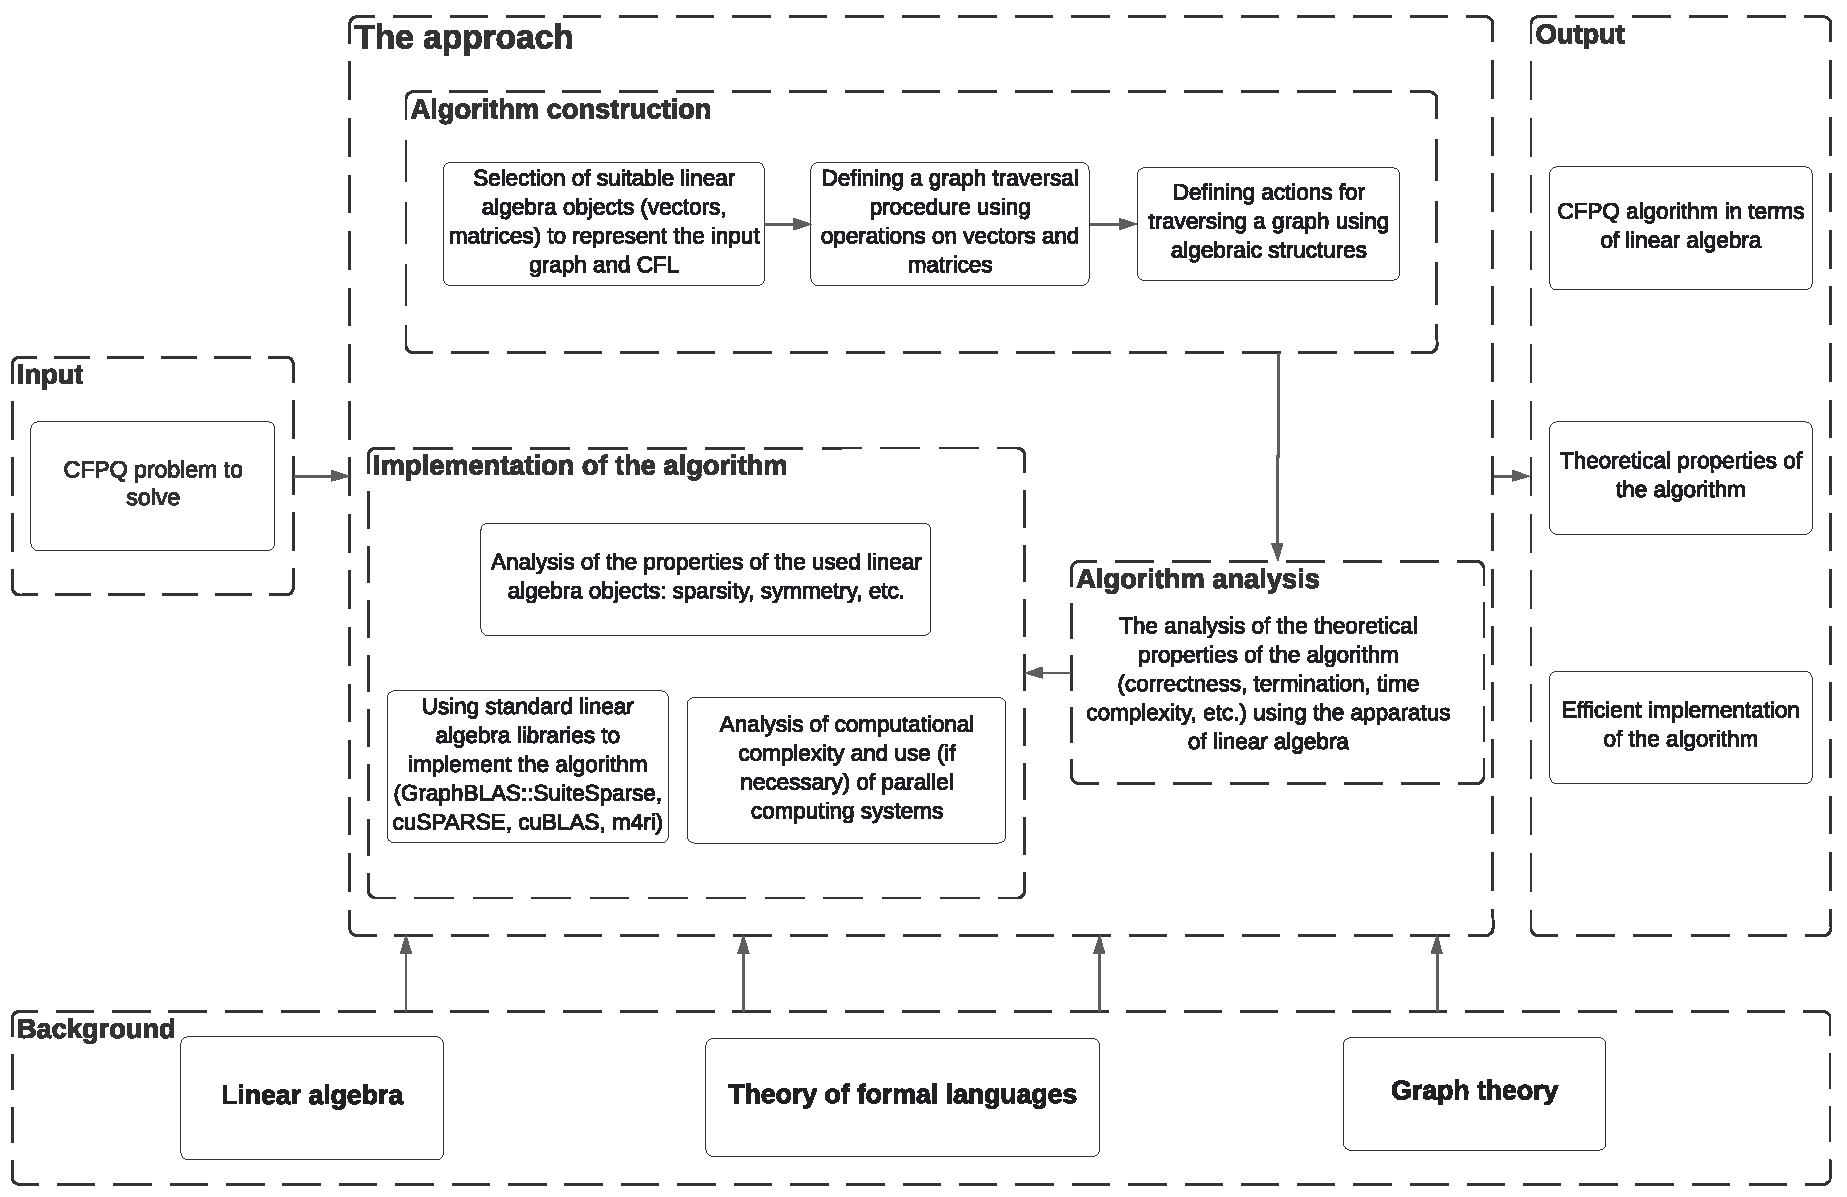
\includegraphics[width = 17.7cm]{Dissertation/images/schema_eng.pdf}
	\caption{A schema of the linear algebra based approach to CFPQ}
	\label{fig:schema}
\end{figure}

%Стоит отметить, что решаемая задача может иметь практическую или теоретическую направленность. Например, при практической направленности целью применения предлагаемого подхода может быть получение высокопроизводительной реализации для решения поставленной задачи анализа графов. А при теоретической направленности основным результатом может являться получение алгоритма, который обладает некоторыми уникальными теоретическими свойствами.
Note that the problem being solved may have a practical or theoretical purpose. For example, with a practical purpose, the goal of applying the proposed approach is to obtain a high-performance implementation of the graph analysis algorithm. And with a theoretical purpose, the main result is to obtain an algorithm that has some unique theoretical properties.

%Также при постановке решаемой задачи может указываться некоторая дополнительная информация про анализируемые графы и используемые КС-ограничения. Например, может быть известна степень разреженности графов или их особый вид (например, что на вход алгоритму будут подаваться только ацикличные графы). Это, в свою очередь, позволит использовать те или иные специфические структуры для хранения информации о графах, а также операции над этими структурами. Для хранения матриц смежности разреженных графов следует выбирать соответствующие разреженные форматы CSR, CSC, COO. А в случае ацикличности графов~--- их матрицы смежности будут иметь треугольный вид, что уменьшит сложность вычисления некоторых операций над ними. Например, первый этап метода Гаусса для решения системы линейных уравнений может быть пропущен, так как он приводит матрицу к треугольной форме. А такая операция, как вычисление транзитивного замыкания для треугольной матрицы имеет сложность, равную сложности вычисления одного умножения матриц. Аналогично, могут быть учтены особенности КС-языков, используемых в качестве КС-ограничений, для поиска наиболее подходящей структуры хранения этих ограничений и операций над этой структурой. Так, если перевод формальной грамматики для заданного КС-языка приводит к слишком значительному увеличению размеров этой грамматики, то целесообразно вместо такой трансформации использовать представление КС-языка в виде рекурсивного автомата. Кроме того, если заданные КС-ограничения соответствуют некоторому подклассу класса КС-языков (например, регулярным языкам), то целесообразно использовать соответствующие более простые структуры (например, конечные автоматы) для описания таких ограничений.
Also, some additional information about the analyzed graphs and the used context-free path constraints can be indicated. For example, the input graph sparsity or special form of the input graph may be known (for example, that only acyclic graphs will be given to the algorithm as input). This, in turn, allows one to use specific structures to store information about graphs, as well as operations on these structures. To store adjacency matrices of sparse graphs, one should choose the appropriate sparse formats CSR, CSC, COO. And in the case of acyclicity of graphs their adjacency matrices will have a triangular form that will reduce the complexity of calculating some operations on them. For example, the first step of the Gauss-Jordan elimination for solving a system of linear equations can be skipped, since it transforms the matrix to a triangular form. And such an operation as the transitive closure calculation for a triangular matrix has a complexity equal to the complexity of calculating a single matrix multiplication. Similarly, the properties of the CFLs used as path constraints can be taken into account in order to find the most appropriate structure for storing these constraints. So, if the normalization of a formal grammar for a given CFL leads to a significant increase of the grammar size then it is advisable to use the representation of the CFL in the form of a recursive automaton. In addition, if the given constraints correspond to some subclass of the class of CFLs (for example, regular languages) then it is advisable to use the corresponding simpler structures (for example, finite automata) to describe such constraints.

The proposed approach is divided into the following parts:
\begin{itemize}
    \item a construction of a CFPQ algorithm in terms of linear algebra;
    \item an analysis of the theoretical properties of the constructed algorithm and the given problem;
    \item an implementation of the constructed algorithm.
\end{itemize}

%Важной частью предлагаемого подхода является само построение алгоритма. Как и при решении других задач анализа графов, ключевым здесь является выбор подходящих объектов линейной алгебры (векторов, матриц) для представления информации о графах. Также подобные объекты можно использовать для представления КС-ограничений путём сведения КС-языков к рекурсивным автоматам~\cite{alur2005analysis} с последующим представлением этих автоматов в виде графов. Для представления информации о графах в подавляющем большинстве алгебраических алгоритмов анализа графов используются матрицы смежности (алгоритм обхода в ширину, алгоритм Беллмана-Форда, алгоритм Флойда-Уоршалла)~\cite{kepner2011graph}. Однако в некоторых из них также используются вектора (в алгоритме Беллмана-Форда для хранения расстояний от стартовой вершины до всех остальных; в алгоритме обхода в ширину один вектор~--- для хранения набора вершин, обрабатываемых на текущей итерации, другой~--- для хранения информации о всех вершинах графа, достижимых из стартовой). Таким образом, для представления графов следует использовать матрицы смежности, а для хранения информации о вершинах графа (достижимость из стартовой вершины; расстояние от стартовой вершины; набор вершин, инцидентных заданной вершине) следует использовать вектора.
An important part of the proposed approach is the algorithm construction. The most important here is the choice of suitable linear algebra objects (vectors, matrices) to represent information about graphs. Also, such objects can be used to represent the context-free path constraints by reducing CFLs to recursive automata~\cite{alur2005analysis} with subsequent representation of these automata as graphs. The majority of algebraic graph analysis algorithms (breadth-first search algorithm, Bellman-Ford algorithm, Floyd-Warshall algorithm)~\cite{kepner2011graph} use adjacency matrices to represent information about graphs. However, some of them also use vectors (in the Bellman-Ford algorithm a vector is used to store the distances from the starting vertex to all the others; in the breadth-first search algorithm, one vector is used to store the set of vertices processed at the current iteration, another vector is used to store information about all graph vertices reachable from the starting one). Thus, adjacency matrices should be used to represent graphs, and vectors should be used to store information about graph vertices (reachability from the starting vertex; distance from the starting vertex; set of vertices incident to a given vertex).


%Далее необходимо задать процедуру обхода графа. Как уже указывалось выше, при удачном выборе объектов линейной алгебры на предыдущем шаге  эта процедура может быть осуществлёна с помощью  операций над выбранными объектами~--- операциями над матрицами и векторами. Так, например, в алгоритме поиска транзитивного замыкания~\cite{baras2010path} для обхода графа используется ряд умножений матриц, а именно, возведений матриц во вторую степень. А в алгоритме Беллмана-Форда~\cite{kepner2011graph} на каждой итерации рассматриваются пути определённой длины с помощью умножения вектора на матрицу смежности. Следует отметить, что в алгоритмах поиска путей между всеми парами вершин используется умножение матрицы на матрицу, а в случае фиксированной стартовой вершины обход графа осуществляется с использованием умножения вектора на матрицу.
Next, we need to specify a graph traversal procedure. As mentioned above, if suitable linear algebra objects was selected then this procedure can be formulated using operations on these objects (vector and matrix operations). For example, in the algorithm for computing the transitive closure~\cite{baras2010path} a repeated squaring of a matrix is used to traverse a graph. And in the Bellman-Ford~\cite{kepner2011graph} algorithm, paths of a certain length are traversed at each iteration by multiplying a vector by an adjacency matrix. Note that algorithms for finding paths between all graph vertices use matrix-matrix multiplication, and in the case of a fixed starting vertex, the graph can be traversed using vector-matrix multiplication.

%Далее, при успешном выполнении предыдущего шага, необходимо задать дополнительные действия в процессе обхода графа, позволяющие анализировать рассматриваемые пути и проверять их на соответствие заданным КС-ограничениям. Здесь предлагается рассмотреть алгебраические структуры, над которыми будут существовать введенные выше объекты линейной алгебры.
Further, it is necessary to set additional actions in the process of graph traversing, which allow one to analyze the visited paths and check them for compliance with the given context-free path constraints. We propose to consider algebraic structures over the linear algebra objects discussed above.

%Эти действия могут быть выполнены путём модификации выбранных операций над матрицами и векторами с использованием различных алгебраических структур (полуколец, моноидов и т.д.). Такие модификации с помощью полуколец широко используются для решения задач поиска путей и являются основной идеей подхода \textit{Algebraic Path Problem}~\cite{rote1990path}. Например, в алгоритме Беллмана-Форда для модификации операции умножения вектора на матрицу используется полукольцо $\langle \mathbb{R} \cup \{\infty\}, min, +, \infty, 0 \rangle$. Также для этого подхода известно много полуколец, которые используются для решения различных задач поиска путей в графе, возникающих в области сетевого анализа~\cite{baras2010path}. Стоит отметить, что в отличии от подхода \textit{Algebraic Path Problem} предлагаемый подход не ограничивается использованием полуколец для переопределения операций линейной алгебры. Например, Лэсли Вэлиант в своем исследовании о синтаксическом анализе строк для КС-грамматик~\cite{valiant1975general} показал как может быть использована алгебраическая структура, схожая с полукольцом, но без требования ассоциативности операции умножения $\otimes$.
These actions can be performed by modifying selected operations on matrices and vectors using various algebraic structures (semirings, monoids, etc.). Such semiring modifications are widely used for solving path querying problems and form the main idea of the \textit{algebraic path problems}~\cite{rote1990path} approach. For example, in the Bellman-Ford algorithm, the semiring $\langle \mathbb{R} \cup \{\infty\}, min, +, \infty \rangle$ is used to define the vector-matrix multiplication. Also, many semirings are known for this approach, which are used to solve various path querying problems that arise in the network analysis~\cite{baras2010path}. Note that, unlike the \textit{algebraic path problems} approach, the proposed approach is not limited to using semirings for modifying the linear algebra operations. For example, Leslie Valiant, in his study of string parsing for the context-free grammars~\cite{valiant1975general}, showed how an algebraic structure similar to a semiring can be used. This structure uses non-associative multiplication operation $\otimes$.

%Построенные алгоритмы могут иметь уникальные теоретические свойства, что может являться основной причиной применения предлагаемого подхода для некоторой поставленной задачи. Поэтому ещё одной важной частью подхода является анализ этих свойств.  Например, Лэсли Вэлиант в работе~\cite{valiant1975general} создал первый субкубический алгоритм синтаксического анализа строк для КС-грамматик. Это стало возможным благодаря формулированию алгоритма синтаксического анализа с помощью методов линейной алгебры и эффективному вычислению использованных алгебраических операций. Таким образом, формулирование алгоритма с использованием методов линейной алгебры даёт возможность также получить теоретический результат и для самой задачи, ответив на некоторый открытый теоретический вопрос в этой области. Одним из таких вопросов является получение алгоритма для задачи поиска путей в графе с заданными КС-ограничениями, имеющего субкубическую сложность ($О(n^{3 - \varepsilon}$), где n~--- количество вершин анализируемого графа, $\varepsilon > 0$). %Или, используя нижние оценки сложности для решаемой задачи поиска путей в графе, возможно удастся доказать новые нижние оценки сложности для некоторых задач линейной алгебры, в случае, если предлагаемый подход позволит свести поставленную задачу анализа графов к этим задачам линейной алгебры.
The constructed algorithms may have unique theoretical properties, which may be the main reason for applying the proposed approach to a given problem. Therefore, another important part of the approach is the analysis of these properties. For example, Leslie Valiant in his work~\cite{valiant1975general} created the first subcubic parsing algorithm for the context-free grammars. This became possible due to the formulation of the parsing algorithm using linear algebra methods and the efficient calculation of the used algebraic operations. Thus, the formulation of an algorithm in terms of linear algebra also makes it possible to obtain a theoretical result for the problem itself, by answering some open theoretical question in this area. One of such open problems is obtaining a subcubic algorithm for the CFPQ problem with the reachability query semantics and with complexity $O(n^{3 - \varepsilon})$ where $n$ is the number of vertices of the analyzed graph and $\varepsilon > 0$.

%С практической точки зрения, важной частью предлагаемого подхода является реализация построенного алгоритма. Такие алгоритмы просты в реализации, так как самым трудоёмким является эффективная реализация необходимых операций линейной алгебры, которые уже реализованы в готовых библиотеках. Основные библиотеки линейной алгебры обсуждались в~\cref{sec:ch1/sec7}, а их характеристики представлены в~\cref{tab:LAlibraries}.
From a practical point of view, an important part of the proposed approach is the implementation of the constructed algorithm. Such algorithms are easy to implement since the most difficult part is to effectively implement the calculation of the necessary linear algebra operations that are already implemented in existing libraries. The existing linear algebra libraries were discussed in section~\ref{sec:ch1/sec7}, and their characteristics are presented in Table~\ref{tab:LAlibraries}.

%Так как данные на практике разрежены, то данные объекты хранятся с использованием разреженных форматов. Например, при выборе матриц смежности входных графов в качестве объектов линейной алгебры используются форматы CSR и CSC для разреженных графов, и формат COO для сильно разреженных графов, когда количество дуг $e \ll n$, где $n$~--- количество вершин графа.
Since graphs are sparse in practice, it is important to store these objects using sparse formats. For example, when choosing adjacency matrices of input graphs as linear algebra objects, the CSR and CSC formats are used for sparse graphs, and the COO format is used for hypersparse graphs. Also, some linear algebra operations can be efficiently computed in parallel. Therefore, the constructed algorithms can be effectively implemented in parallel on the CPU, GPU, using distributed computing, etc. Depending on the selected linear algebra operations, the object storage format, and the selected computing system, the choice of the appropriate linear algebra library is made. Also, the selected operations can be implemented independently.

%При практической направленности поставленной задачи выбор самих объектов линейной алгебры, формата их хранения и операций над ними может быть основан на получении наиболее высокопроизводительной реализации, которые смогут решать задачу поиска путей с заданными КС-ограничениями на графах с миллионами дуг за десятки секунд. В работе~\cite{kuijpers2019experimental} было проведено исследование, которое показало, что реализации основных существующих алгоритмов для задачи достижимости с заданными КС-ограничениями недостаточно производительны для использования на практике.
%With the practical orientation of the given problem, the choice of the linear algebra objects themselves, their storage format and operations on them can be based on obtaining the most high-performance implementation that can solve the CFPQ problem on graphs with millions of edges in tens of seconds. In the work~\cite{kuijpers2019experimental}, a study was conducted that showed that the implementations of the state-of-art reachability CFPQ algorithms are not performant enough to be used in practice.



%В большинстве случаев задачи анализа графов можно решить с использованием операций над набором булевых матриц и векторов. Тогда для эффективного параллельного вычисления операций над разреженными булевыми матрицами на CPU рекомендуется использовать библиотеку SuiteSparse:GraphBLAS (реализацию стандарта GraphBLAS). Кроме того, в этой библиотеке для матриц и векторов можно определить пользовательский тип данных, с помощью которого могут быть решены более сложные задачи, например, задача поиска всех путей в графе с заданными КС-ограничениями. В то же время насколько известно автору не существует библиотеки линейной алгебры, предлагающей возможность вычисления операций над матрицами и векторами на GPU над пользовательскими типами данных. Однако существуют библиотеки cuSPARSE, cuBool и GraphBLAST, с реализованными операциями над разреженными матрицами и векторами на GPU. Хотя для алгоритмов поиска путей в графе, которые удаётся сформулировать с использованием операций над набором булевых матриц, не рекомендуется использовать библиотеку cuSPARSE, так как в ней не реализованы специальные функции для вычисления операций над булевыми матрицами и векторами. В таком случае в библиотеке cuSPARSE придётся использовать в качестве типа данных числа с плавающей точкой, что существенно скажется на затратах по памяти и времени работы реализации.
Some graph analysis problems can be solved using operations on a set of Boolean matrices and vectors. In such cases, for efficient parallel computation of operations on sparse Boolean matrices on CPU it is recommended to use the SuiteSparse:GraphBLAS library (implementation of the GraphBLAS standard). In addition, this library allows one to use user-defined data types to solve more complex problems, for example, the CFPQ problem with the all-path query semantics. Moreover, cuSPARSE, cuBool, GraphBLAST, and CUSP libraries with implemented operations on sparse matrices and vectors can be used to obtain GPU implementations. Note that the cuSPARSE library does not provide special operations on Boolean matrices and vectors. Therefore, to calculate operations on Boolean matrices and vectors using this library, the floating-point numbers should be used as a data type, which will significantly affect the memory cost and running time of the implementation.

As a result, the proposed approach makes it possible to obtain one or more of the following results:
\begin{itemize}
    \item a CFPQ algorithm in terms of linear algebra;
    \item theoretical properties of the constructed algorithm and the solved CFPQ problem;
    \item an efficient implementation of the constructed algorithm.
\end{itemize}

\section{An Example of Constructing an Algorithm}\label{sec:ch2/sec2}

%Для демонстрации применения предложенного подхода рассмотрим построение алгоритма для частного случая задачи поиска путей в графе с заданными КС-ограничениями, в котором ограничения задаются строгим подклассом КС-языков~--- регулярными языками, а сама задача является задачей достижимости. В данной задаче на вход подаётся помеченный граф и регулярный язык, описывающий ограничения на пути в нём.
To demonstrate the application of the proposed approach, consider the construction of an algorithm for a partial case of the CFPQ problem with the reachability query semantics, in which the constraints are given by a strict subclass of CFLs~--- regular languages. In this problem, the input is a labeled graph and a regular language that describes the path constraints.

%Сначала необходимо определиться с использованием объектов линейной алгебры для представления входного графа и регулярного языка. В теории формальных языков существует теорема Клини~\cite{hopcroft2001introduction}, согласно которой класс регулярных языков совпадает с классом языков, распознаваемых конечными автоматами. Поэтому одним из способов задания регулярных языков является построение соответствующего конечного автомата. В свою очередь входной помеченный граф также может быть представлен в виде конечного автомата, у которого все состояния являются и стартовыми и финальными. Тогда поставленную задачу достижимости с заданными ограничениями можно решить путём нахождения пересечения этих двух конечных автоматов. По теореме~\ref{thm:FAintersection_and_kron}, вычислять пересечение конечных автоматов можно с использованием произведения Кронекера, применённого к матрицам из булевых декомпозиций матриц смежности для графовых представлений этих автоматов. Таким образом, входные граф и регулряный язык будут представлены в виде набора булевых матриц, а процедурой обхода графа будет являться ряд произведений Кронекера булевых матриц.
First, it is necessary to select linear algebra objects to represent information about the input graph and the regular language. One of the ways to define a regular language is to construct an appropriate finite automaton~\cite{hopcroft2001introduction}. In turn, the input labeled graph can also be represented as a finite automaton, in which all states are both initial and final. Then the stated reachability problem with given constraints can be solved by finding the intersection of these two finite automata, as well as by solving the reachability problem for the graph representation of this intersection via the transitive closure calculation. According to the theorem~\ref{thm:FAintersection_and_kron}, the intersection of finite automata can be calculated using the Kronecker product applied to matrices from Boolean decompositions of adjacency matrices for graph representations of these automata. Thus, the input graph and regular language will be represented as a set of Boolean matrices, and the graph traversal procedure will be a series of Kronecker products of Boolean matrices followed by a transitive closure calculation.

%Пусть конечный автомат $F_1$ описывает входной граф, а $F_2$~--- входной регулярный язык. Тогда на листинге~\ref{lst:fsa_intersection} приведён алгоритм, использующий методы линейной алгебры для решения задачи достижимости с заданными ограничениями в виде регулярного языка. В строке 7 алгоритм производит обход графа с использованием произведения Кронекера, в результате которого будет построена матрица переходов конечного автомата $F$, являющегося пересечением конечных автоматов $F_1$ и $F_2$. Здесь булевы матрицы $M_i^a$ хранят в себе информацию о переходах с символом $a$ в автомате $F_i$. Затем в строке 8 вычисляется матрица $M^*$, которая содержит информацию о всех общих путях в графах, соответствующих конечным автоматам $F_1$ и $F_2$. Для этого используется функция $\textit{transitiveClosure}$ и операция $\bigvee$ поэлементной дизъюнкции булевых матриц. Стоит отметить, что функция $\textit{transitiveClosure}$ также может быть реализована с использованием методов линейной алгебры, а именно через серию возведений передаваемой булевой матрицы во вторую степень. И, наконец, в строках 9--12 вычисляется множество $\textit{result}$, являющееся ответом на задачу достижимости в графе с ограничениями в виде регулярного языка. При этом используется тот факт, что наличие в ячейке $M^*[(i, s_1), (j, s_2)]$ значения 1 эквивалентно существованию пути $\pi_1$ во входном графе из вершины $i$ в вершину $j$, и пути $\pi_2$ в графовом представлении конечного автомата $F_2$ из вершины $s_1$ в вершину $s_2$, где $\lambda(\pi_1) = \lambda(\pi_2)$. Это означает, что для любой пары вершин $(i, j)$ входного графа, вершина $j$ достижима из вершины $i$ хотя бы одним путём, удовлетворяющим входным ограничениям тогда и только тогда, когда $M^*[(i, s_1), (j, s_2)] = 1$ для вершины $s_1$, соответствующей начальному состоянию конечного автомата $F_2$, и вершины $s_2$, соответствующей одному из его конечных состояний. Таким образом, построенный алгоритм решает поставленную задачу анализа графов.
Suppose that the finite automaton $F_1$ describes the input graph, and $F_2$~--- the input regular language. The Listing~\ref{lst:fsa_intersection} provides an algorithm that uses linear algebra methods to solve the reachability problem with given path constraints in the form of a regular language. In the line 7, the algorithm traverses the graph using the Kronecker product, as a result of which the transition matrix of the finite automaton $F$ will be built, which is the intersection of the finite automata $F_1$ and $F_2$. Here Boolean matrices $M_i^a$ store information about transitions with symbol $a$ in automaton $F_i$. Then, in the line 8, the matrix $M^*$ is calculated, which contains information about all paths in the input graph corresponding to the given path constraints. For this, the $\textit{transitiveClosure}$ function and the element-wise addition operation $\bigvee$ defined over the Boolean semiring $\langle \{0, 1\}, \vee, \wedge, 0 \rangle$ are used. Note that the $\textit{transitiveClosure}$ function can also be implemented using linear algebra methods, namely through a repeated squaring of a Boolean matrix. Finally, lines 9-12 calculate the set $\textit{result}$, which is the answer to the reachability problem in a graph with regular language path constraints. Here the value 1 in the cell $M^*[(i, s_1), (j, s_2)]$ indicates the existence of the path $\pi_1$ in the input graph from the vertex $i$ to the vertex $j$, and the existence of the path $\pi_2$ in the graph representation of the finite automaton $F_2$ from vertex $s_1$ to vertex $s_2$ where $\lambda(\pi_1) = \lambda(\pi_2)$. This means that for any pair of vertices $(i, j)$ in the input graph, the vertex $j$ is reachable from the vertex $i$ by at least one path that satisfies the input constraints if and only if $M^*[(i, s_1), (j, s_2)] = 1$ for the vertex $s_1$ corresponding to the initial state of the finite automaton $F_2$ and the vertex $s_2$ corresponding to one of its final states. Thus, the constructed algorithm solves the given graph analysis problem.

\begin{algorithm}
  \floatname{algorithm}{Listing}
\begin{algorithmic}[1]
\caption{A reachability regular path querying algorithm}
\label{lst:fsa_intersection}
\Function{AlgebraicRegularPathQuerying}{$F_1, F_2$}
    \State{$\mathcal{M}_1 \gets$ the Boolean decomposition of the adjacency matrix for $F_1$}
    \State{$\mathcal{M}_2 \gets$ the Boolean decomposition of the adjacency matrix for $F_2$}
    \State{$q_s \gets$ the initial state of the finite automaton $F_2$ describing the regular language}
	\State{$Q_f \gets$ the set of final states of the automaton $F_2$}
    \State{$\Sigma \gets$ the set of common symbols on transitions in automata $F_1$ и $F_2$}
    \State{$\mathcal{M} \gets \{ M_1^a \times M_2^a \mid a \in \Sigma\}$}
    \Comment{\text{The Kronecker product}}
    \State{$M^* \gets \textit{transitiveClosure}(\bigvee_{M \in \mathcal{M}} M)$}
    \State{$\textit{result} \gets \emptyset$}
    \For{$i, j, s \mid M^*[(i, q_s), (j, s)] = 1$}
    \If{$s \in Q_f$}
    \State{$\textit{result} \gets \textit{result} \cup \{(i, j)\}$}
    \EndIf
    \EndFor
    \State \Return \textit{result}
\EndFunction
\end{algorithmic}
\end{algorithm}

%Для решения задачи достижимости была использована операция произведения Кронекера булевых матриц, основанная на стандартных логических операций из булевого полукольца $\langle \{0, 1\}, \vee, \wedge, 0, 1\rangle$. В данном случае не требуется задавать дополнительные действия при обходе графа с помощью изменения этой алгебраической структуры. Однако такие действия могут понадобиться при решении других задач поиска путей в графе, например, при поиске всех путей в графе с заданными КС-ограничениями.
To solve the reachability problem, the Kronecker product of Boolean matrices was used, based on standard logical operations from the Boolean semiring $\langle \{0, 1\}, \vee, \wedge, 0 \rangle$. In this case, it is not required to specify additional actions when traversing the graph by changing this algebraic structure. However, such actions may be needed when solving other path querying problems. For example, when solving path querying problems with the all-path query semantics.

%Таким образом, было показано, как может быть построен алгоритм с использованием методов линейной алгебры для решения задачи достижимости с заданными ограничениями в виде регулярного языка.
Thus, it was shown how a CFPQ algorithm can be constructed using linear algebra methods when path constraints are formulated in the form of a regular language.

\section{On Applicability and Limitations of the Approach}
%Далеко не каждый алгоритм анализа графов и, в частности, алгоритм поиска путей в графе, удаётся сформулировать в терминах линейной алгебры. Например, было сделано много попыток найти такую формулировку для алгоритма поиска в глубину~--- этот алгоритм является  одним из фундаментальных алгоритмов анализа графов. Однако недавно это удалось сделать лишь для частных случаев графов (двоичного дерева, ациклического графа)~\cite{spampinato2019linear}. В свою очередь, алгоритм поиска в ширину легко может быть сформулирован в терминах линейной алгебры и такая формулировка была давно найдена~\cite{kepner2011graph}.
Not every graph analysis algorithm, in particular, a path querying algorithm, can be formulated in terms of linear algebra. For example, many attempts have been made to find such a formulation for the depth-first search algorithm~--- this algorithm is one of the fundamental graph analysis algorithms. However, recently such a formulation was found only for particular cases of graphs (for binary trees, acyclic graphs)~\cite{spampinato2019linear}. In turn, the breadth-first search algorithm can be easily formulated in terms of linear algebra, and such a formulation was found a long time ago~\cite{kepner2011graph}.

%Таким образом,  при применении предложенного подхода на этапе построения алгоритма могут возникнуть следующие проблемы:
Thus, when applying the proposed approach at the stage of constructing the algorithm, the following issues may arise:

\begin{itemize}
    \item the challenge of formulating a graph traversal procedure using operations on selected linear algebra objects;
    \item the challenge of finding algebraic structures for additional actions that are necessary for the stated graph analysis problem during the graph traversal.
\end{itemize}

%При неудачном решении этих проблем необходимо вернуться к выбору объектов линейной алгебры. Такой возврат  также необходим при выявлении проблем на более поздних этапах подхода. Например, на этапе анализа теоретических свойств построенного алгоритма может быть выявлена неудовлетворительная временная сложность алгоритма. В то же время на этапе реализации может возникнуть сложность написания собственной реализации построенного алгоритма или следующие проблемы, связанные с использованием стандартных библиотек линейной алгебры:
In case of failure in solving these issues, it is necessary to return to the choice of linear algebra objects. Such a return is also necessary when issues are identified at later stages of the approach. For example, the unsatisfactory time complexity of the constructed algorithm can be identified at the stage of analyzing the theoretical properties. At the same time, at the implementation stage, it may be difficult to use standard linear algebra libraries:
\begin{itemize}
    \item the properties of the linear algebra objects used to represent them do not allow one to use existing linear algebra libraries;
    \item unsatisfactory running time or high memory consumption of the implementation were detected.
\end{itemize}

%Стоит также отметить, что не все этапы подхода являются обязательными. Например, при практической направленности решаемой задачи может быть пропущен этап анализа теоретических свойств алгоритма, а при выборе используемых объектов линейной алгебры и операций над ними необходимо руководствоваться возможностями существующих библиотек линейной алгебры. С другой стороны, при теоретической направленности решаемой задачи может отсутствовать этап реализации построенного алгоритма, а на этапе построения алгоритма необходимо выбрать подходящие объекты линейной алгебры и операции над ними для получения наилучших теоретических свойств алгоритма.
Note that not all stages of the approach are mandatory. For example, in the case of the practical purpose of the problem being solved, the stage of analyzing the theoretical properties of the algorithm can be skipped, and when choosing the linear algebra objects and operations, it is necessary to be guided by the properties of existing linear algebra libraries. On the other hand, when the problem being solved has theoretical purpose, there may be no stage of implementing the constructed algorithm, and at the stage of constructing the algorithm, it is necessary to select suitable linear algebra objects and operations to obtain the best theoretical properties of the algorithm.

\section{Summary}
%Таким образом, в данной главе представлен подход к поиску путей в произвольном графе с заданными произвольными КС-ограничениями с использованием методов линейной алгебры. Новизна подхода заключается в следующем.
Thus, in this chapter, we proposed a linear algebra based approach to CFPQ. The novelty of this approach is as follows.
\begin{enumerate}
    \item The existing CFPQ approaches either do not use linear algebra methods or are intended only for a partial case of the context-free path constraints and/or for specialized graphs.
    \item The proposed approach allows one to use a wide class of optimizations of linear algebra operations for efficient analysis of large graphs.
    \item The proposed approach makes it possible to build algorithms that are easy to implement, portable, and allow one to use parallel computations and existing linear algebra libraries.
\end{enumerate}

\FloatBarrier
           % Глава 2
\chapter{Алгоритм поиска путей в графе с заданными КС-ограничениями с использованием операций умножения матриц}\label{ch:ch3}
В данной главе изложен алгоритм, полученный в результате применения подхода из предыдущей главы для решения задачи достижимости, поиска одного и поиска всех путей в графе с заданными КС-ограничениями с использованием операций умножения матриц. Также сформулированы и доказаны утверждения о корректности и временной сложности полученного алгоритма. Кроме того, приведены детали реализаций алгоритма, а также его работа продемонстрирована на примере.
\section{Построение алгоритма}\label{sec:ch3/sect1}
В данном разделе изложен процесс построения алгоритма поиска путей в графе с заданными КС-ограничениями с использованием операций умножения матриц.

Пусть дан входной помеченный граф $\mathcal{G} = \langle V, E, L\rangle$ и входной КС-язык в качестве ограничений на пути в нём. Сперва необходимо выбрать объекты линейной алгебры для представления информации о графе. Применимость таких объектов линейной алгебры, как матрицы в задачах анализа графов давно известна. Поэтому для представления входного графа будем использовать его матрицу смежности, в ячейках $(i, j)$ которой будет содержаться информация о дугах между вершиной $i$ и вершиной $j$. Входной КС-язык будем описывать КС-грамматикой $G = \langle \Sigma, N, P, S \rangle$ в ослабленной нормальной форме Хомского, которая, как мы увидим, будет удобна для дальнейшего построения алгебраических структур с операциями, учитывающими заданные КС-ограничения в процессе поиска путей в графе. Затем матрицу смежности необходимо инициализировать, включив в неё информацию о заданных ограничениях. Для описания связи найденных путей в графе с заданными КС-ограничениями будут использоваться нетерминальные символы грамматики $G$. Таким образом, в процессе работы предлагаемый алгоритм для всех рассматриваемых путей $\pi$ будет выяснять из каких нетерминалов $A$ выводится строка $\lambda(\pi)$. Поэтому для инициализации матрицы смежности входного графа будут рассмотрены все дуги с метками $a \in \Sigma \cap L$ и соответствующие им правила вида $A \rightarrow a$. Таким образом, будут рассмотрены все пути графа длины 1, но также необходимо рассмотреть пустые пути, при условии наличия в грамматике $G$ правил вида $A \rightarrow \varepsilon$. Поэтому для каждого такого правила и для каждой вершины $i$ графа $\mathcal{G}$ в матрицу будет записана информация о наличии пустого пути $\pi$ из вершины $i$ в вершину $i$ такого, что строка $\lambda(\pi)$ выводится из нетерминала $A$.

Далее опишем процедуру обхода графа, основанную на вычислении транзитивного замыкания инициализированной матрицы. Такое транзитивное замыкание может быть вычислено с использованием известной техники~\cite{baras2010path}, в которой производится серия умножений матрицы смежности на себя. Это позволит обойти граф и рассмотреть все необходимые для анализа графа пути. Остаётся лишь переопределить операцию умножения таких матриц, чтобы, во-первых, в процессе обхода графа рассматриваемые пути проверялись на соответствие входным КС-ограничениям, а, во-вторых, вычислялась вся необходимая информация для решения поставленной задачи достижимости, поиска одного или поиска всех путей в графе. Для проверки путей на соответствие входным КС-ограничениям будут использованы правила вида $A \rightarrow B C$, где $A, B, C \in N$. В правой части таких правил имеется лишь конкатенация двух нетерминалов, что в процессе вывода строки в грамматике соответствует конкатенации двух подстрок. Аналогично, в процессе анализа графа правила такого вида соответствуют конкатенации двух коротких путей $i \pi_1 k$ и $k \pi_2 j$, где $B \Rightarrow_G \lambda(\pi_1)$ и $C \Rightarrow_G \lambda(\pi_2)$. В таком случае, для пути $i\pi j$, полученного в результате такой конкатенации мы можем утверждать, что $A \Rightarrow_G \lambda(\pi)$. Таким образом, процесс обхода графа $\mathcal{G}$ будет неразрывно связан с процессом вывода строк в грамматике $G$, образованных рассмотренными путями графа. И, наконец, чтобы вычислялась вся необходимая информация для решения поставленной задачи поиска путей в графе, построим алгебраическую структуру $\langle \textit{MatrixElements}, \oplus, \otimes, \bot \rangle$, где:
\begin{itemize}
    \item $\textit{MatrixElements}$~--- множество, содержащее в себе все возможные значения элементов рассматриваемых матриц;
    \item $\oplus$~--- операция сложения элементов матриц, которая будет использоваться при агрегации информации о нескольких путях в графе между одними и теми же вершинами;
    \item $\otimes$~--- операция умножения элементов матриц, которая будет использоваться при агрегации информации о двух путях, которые могут быть сконкатенированы в один более длинный путь;
    \item $\bot$~--- нейтральный по сложению элемент, который будет обозначать отсутствие искомых путей для конкретной пары вершин.
\end{itemize}

Тогда используя построенную алгебраическую структуру определим операцию умножения матриц \mbox{$a \cdot b = c$}, где $a$ и $b$~--- матрицы подходящих размеров с элементами из множества $\textit{MatrixElements}$, как $$c_{i, j} = \bigoplus^{n}_{k=1}{a[i, k] \otimes b[k, j]}.$$ Кроме того, для агрегации информации о путях из двух матриц одинакового размера будем использовать операцию $\bigoplus$ поэлементного сложения элементов этих двух матриц, определённую над той же алгебраической структурой. Также на этапе инициализации необходимо определить элементы, используемые для описания информации о путях длины 0 и 1. Так как значения этих элементов зависят от поставленной задачи поиска путей в графе, то обозначим их, как $\alpha^0_{i, j}, \alpha^1_{i, j} \in \textit{MatrixElements}$, для каждой пары вершин $(i, j)$.

Таким образом, на листинге~\ref{lst:mtx_cfpq} представлен алгоритм поиска путей в графе с заданными КС-ограничениями, использующий операции умножения матриц. Представленный алгоритм принимает на вход граф и КС-ограничения уже выраженные в виде КС-грамматики в ослабленной нормальной форме Хомского. Стоит отметить, что вместо одной матрицы информация о путях в графе хранится в множестве матриц $T$, состоящем из $|N|$ матриц $T^A$ по одной на каждый нетерминальный символ $A \in N$. В таком случае в ячейку $T^A[i, j]$ записывается информация о найденных путях в графе из вершины $i$ в вершину $j$, образующих строки, выводимые из нетерминала $A$ в грамматике $G$. Данная идея схожа с идеей использования булевой декомпозиции матрицы смежности, однако получаемые матрицы $T^A$ будут булевыми только для задачи достижимости. В итоге, предложенный алгоритм решает поставленную задачу поиска путей в графе $\mathcal{G}$ с заданными КС-ограничениями, так как вся необходимая информация о путях из вершины $i$ в вершину $j$, удовлетворяющих заданным КС-ограничениям в виде грамматики $G = \langle \Sigma, N, P, S\rangle$, будет записана в ячейку $T^S[i, j]$.


\begin{algorithm}
	\begin{algorithmic}[1]
		\floatname{algorithm}{Листинг}
		\caption{Алгоритм поиска путей в графе с заданными КС-ограничениями, использующий операции умножения матриц}
		\label{lst:mtx_cfpq}
		\Function{MatrixBasedCFPQ}{$\mathcal{G} = \langle V, E, L \rangle$, $G= \langle N, \Sigma, P, S \rangle$}
		\State{$n \gets$ |V|}
		\State{$T \gets \{T^{A} \mid A \in N$, где $T^{A}$~--- матрица размера $n \times n$ со всеми элементами равными $\bot$ \} }
		
		\ForAll{$(i, x, j) \in E$, $A \mid A \to x \in P$}
		%\Comment{Matrices initialization}
		%\For{$A_k \mid A_k \to x \in P$}
		\State{$T^{A}[i, j] \gets \alpha^1_{i, j}$} \Comment{Инициализация матриц для правил вида $A \to x$}
		%\EndFor
		\EndFor
		\For{$A \mid A \to \varepsilon \in P$}
		\ForAll{$i \in \{0,\ldots, n - 1\}$}
		\State{$T^{A}[i, i] \gets \alpha^0_{i, i}$} \Comment{Инициализация матриц для правил вида $A \to \varepsilon$}
		\EndFor
		\EndFor
		
		\While{любая матрица из $T$ меняется}
		%\Comment{Transitive closure calculation}
		\ForAll{$A \to B C \in P$, где $T^{B}$ или $T^{C}$ изменились}
		\State{ $T^{A} \gets T^{A} \bigoplus (T^{B} \cdot T^{C})$ } 
		\EndFor
		\EndWhile
		\State \Return $T$
		\EndFunction
		
	\end{algorithmic}
\end{algorithm}

Далее представим различные алгебраические структуры, позволяющие переопределить операции над матрицами в алгоритме, представленном на листинге~\ref{lst:mtx_cfpq}, для решения задачи достижимости, поиска одного пути или поиска всех путей в графе с заданными КС-ограничениями.

\paragraph{Задача достижимости.} Так как для решения задачи достижимости необходима лишь информация о наличии путей, образующих из меток своих дуг определённые слова, то в ячейках матрицы смежности могут содержаться только булевы значения 0 или 1. В таком случае в ячейку $T^A[i, j]$ записывается значение 1, если существует путь из вершины $i$ в вершину $j$, образующий строку, выводимую из нетерминала $A$ в грамматике $G$, и значение 0 в противном случае. В процессе инициализации матриц в ячейки $T^A[i, j]$ будут записываться значения $\alpha^0_{i, j}$ и $\alpha^1_{i, j}$ при обнаружении соответствующего пути длины 0 или 1. А так как для поставленной задачи наличие пути записывается в соответствующую ячейку с помощью значения 1, то $\alpha^0_{i, j} = \alpha^1_{i, j} = 1$. Таким образом, алгоритм, представленный на листинге~\ref{lst:mtx_cfpq} решает задачу достижимости в графе с заданными КС-ограничениями при использовании алгебраической структуры $\langle \{0, 1\}, \vee, \wedge, 0 \rangle$ с логическими операциями дизъюнкции и конъюнкции. В графе $\mathcal{G}$ существует путь из вершины $i$ в вершину $j$, удовлетворяющий заданным КС-ограничениям, только если $T^S[i, j] = 1$.

\paragraph{Задача поиска одного пути.}
Для решения задачи поиска одного пути в графе с заданными КС-ограничениями, необходимо для каждой пары вершин $(i, j)$ иметь возможность построить хотя бы одни путь из вершины $i$ в вершину $j$, удовлетворяющий заданным ограничениям, если такие пути существуют. Для этого добавим в ячейки матриц дополнительную информацию о найденных путях в графе и построим новую алгебраическую структуру для модификации операций над этими матрицами. Будем использовать матрицы, в ячейках которых записана информация о найденных путях в виде четвёрок ($\textit{left}$, $\textit{right}$, $\textit{middle}$, $\textit{height}$), где $\textit{left}$ и $\textit{right}$~--- конечные вершины найденного пути, $\textit{middle}$~--- одна из промежуточных вершин найденного пути $\pi$ со строкой $\lambda(\pi)$, выводимой из нетерминала $A$ в грамматике $G$, и $\textit{height}$~--- минимальная высота дерева вывода строки $\lambda(\pi)$ из нетерминала $A$. В случае, когда для определенной пары вершин $(i, j)$ таких путей не обнаружено, то будем использовать четвёрку $\bot = (0, 0, 0, 0)$. 

Для конкретной пары вершин $(i, j)$ и нетерминала $A$ в предложенном алгоритме будет рассматриваться путь, образующий строку, выводимую из нетерминала $A$ и имеющую минимальную высоту дерева вывода. Кроме того, будут рассматриваться конкатенации двух таких путей для различных троек $(A, i, j)$. Поэтому в предложенном алгоритме будут использоваться только четвёрки ($\textit{left}$, $\textit{right}$, $\textit{middle}$, $\textit{height}$) с $\textit{height} \leq h + 1$, где $h$~--- максимальная из таких минимальных высот деревьев вывода для различных троек $(A, i, j)$. Обозначим множество всех возможных таких четвёрок, включая $\bot$, как $\textit{PathIndex}$, и построим алгебраическую структуру, используя это множество как носитель. Нейтральным по сложению элементом в такой структуре будет являться четвёрка $\bot$. В таком случае, изначально все матрицы будут инициализированы этим нейтральным элементом. Далее необходимо определить операции умножения и сложения для этой структуры.

Так как в процессе обхода графа с использованием операции умножения матриц и правил грамматики вида $A \to B C$, рассматриваются более длинные пути $i \pi j$, являющиеся конкатенацией двух коротких путей $i\pi_1 k$ и $k \pi_2 j$, то в качестве промежуточной вершины $\textit{middle}$ длинного пути удобно выбрать вершину $k$. Тогда операция умножения $\otimes$ для \mbox{$\textit{PI}_1, \textit{PI}_2 \in \textit{PathIndex}$}, может быть определена следующим образом.

$$\textit{PI}_1 \otimes \textit{PI}_2 = \begin{cases}
      (\textit{PI}_1.\textit{left}, \textit{PI}_2.\textit{right}, \textit{PI}_1.\textit{right}, max(\textit{PI}_1.\textit{height}, \textit{PI}_2.\textit{height}) + 1),\\
                     \qquad \text{если $\textit{PI}_1\neq \bot \neq \textit{PI}_2$} \\
      \bot, \qquad \text{иначе} \\
    \end{cases}\
$$

Кроме того, в процессе анализа графа для одной и той же пары вершин могут быть найдены несколько путей, удовлетворяющих заданным КС-ограничениям. Такие пути агрегируются с использованием операции сложения $\oplus$ для \mbox{$\textit{PI}_1, \textit{PI}_2 \in \textit{PathIndex}$}, которая может быть определена следующим образом.

$$\textit{PI}_1 \oplus \textit{PI}_2 = \begin{cases}
      \textit{PI}_1, \qquad \text{если $\textit{PI}_1\neq \bot \neq \textit{PI}_2$ и} \\ \qquad (\textit{PI}_1.\textit{height}, \textit{PI}_1.\textit{middle}) \leq (\textit{PI}_2.\textit{height}, \textit{PI}_2.\textit{middle}) \\
      \textit{PI}_1, \qquad \text{если $\textit{PI}_2 = \bot$} \\
      \textit{PI}_2, \qquad \text{иначе} \\
    \end{cases}\
$$

В представленном определении использовался лексикографический порядок над парами целых чисел $(\textit{PI}.\textit{height}, \textit{PI}.\textit{middle})$ для $\textit{PI} \in \textit{PathIndex}$. Таким образом, при использовании операции $\oplus$ в ячейках матрицы $T^A$ будет содержаться информация о найденных путях, образующих строки с минимальными высотами деревьев вывода из нетерминала $A$ в грамматике $G$. Далее определим значения элементов $\alpha^0_{i, j}, \alpha^1_{i, j} \in \textit{PathIndex}$. При обнаружении пути длины 1, выводимого из нетермниала $A_k$ в соответствующую ячейку матрицы $T^{A_k}$ будет добавляться информация об этом пути в виде четвёрки $\alpha^1_{i, j} = (i, j, i, 1)$. В свою очередь для путей длины 0 в соответствующие ячейки добавляются четвёрки $\alpha^0_{i, i} = (i, i, i, 1)$. В данных случаях в качестве промежуточных вершины выбраны начальные вершины путей длины 0 и 1. Таким образом, алгоритм, представленный на листинге~\ref{lst:mtx_cfpq} позволяет решить задачу поиска одного пути в графе с заданными КС-ограничениями при использовании полукольца $\langle \textit{PathIndex}, \oplus, \otimes, \bot \rangle$ с определенными для данной задачи операциями. Результатом работы алгоритма является множество матриц $T^A$ для всех нетерминальных символов $A \in N$, в ячейках $(i, j)$ которых содержится информация об одном найденном пути из вершины $i$ в вершину $j$, образующем строку, выводимую из нетерминала $A$ с минимальной высотой дерева вывода. В случае, если для пары вершин $(i, j)$ таких путей не существует, то $T^A[i, j] = \bot$.

Однако кроме построения множества матриц $T$, содержащих информацию о найденных путях, необходимо восстановить путь $i \pi j$ для любых $i, j$ и нетерминала $A$ таких, что $A \Rightarrow_G \lambda(\pi)$, если такой путь существует. Поэтому на листинге~\ref{lst:mtx_single_extract} представлен алгоритм восстановления одного пути, соответствующего заданным КС-ограничениям, для любой пары вершин $(i, j)$ и нетерминала $A$. Представленный алгоритм восстанавливает путь, соответствующий строке с минимальной высотой дерева вывода. Алгоритм возвращает пустой путь $\pi_{\varepsilon}$ только когда $i = j$ и $A \to \varepsilon \in P$. Необходимо заметить, что если $T^A[i, j] = \bot$, то предложенный алгоритм возвращает специальный путь $\pi_{\emptyset}$, обозначающий отсутствие путей соответствующих заданным КС-ограничениям.

	\begin{algorithm}
		\floatname{algorithm}{Листинг}
		\begin{algorithmic}[1]
			\caption{Алгоритм восстановления одного пути в графе с заданными КС-ограничениями}
			\label{lst:mtx_single_extract}
			\Function{ExtractSinglePath}{$i, j, A, T=\{T^{A_i}\}, G=\langle N, \Sigma, P, S \rangle$}
			\State{$\textit{index} \gets T^{A}_{i,j}$ }
			
			\If{$\textit{index} = \bot$}
			\State \Return $\pi_{\emptyset}$
			\Comment{Такого пути не существует}
			\EndIf
			
			\If{$\textit{index.height} = 1$}
			\If{$(i = j) \wedge (A \to \varepsilon \in P)$}
			\State \Return $\pi_{\varepsilon}$
			\Comment{Возвращаем пустой путь}
			\EndIf
			\ForAll{$ x \mid (i,x,j) \in E$}
			\If{$A \to x \in P$}
			\State \Return $[(i,x,j)]$
			\Comment{Возвращаем путь длины 1}
			\EndIf
			\EndFor
			\EndIf
			
			\ForAll{$A \to B C \in P$}
			\State{$\textit{index}_B \gets T^{B}[i, \textit{index.middle}]$ }
			\State{$\textit{index}_C \gets T^{C}[\textit{index.middle}, j]$ }			
			\If{$(\textit{index}_B \neq \bot) \wedge (\textit{index}_C \neq \bot)$}
			\State{$\textit{maxH} \gets \textit{max}(\textit{index}_B.\textit{height}, \textit{index}_C.\textit{height})$ }
			\If{$\textit{index.height} = \textit{maxH} + 1$}
			
						
			\State{$\pi_1 \gets$ \Call{ExtractSinglePath}{$i, \textit{index.middle}, B, T, G$}}
			\State{$\pi_2 \gets$ \Call{ExtractSinglePath}{$\textit{index.middle}, j, C, T, G$}}
			\State \Return $\pi_1 + \pi_2$
			\Comment{Возвращаем конкатенацию двух путей}
			\EndIf
			\EndIf
			\EndFor
			\EndFunction
		\end{algorithmic}
	\end{algorithm}
	
Таким образом, алгоритмы представленные на листингах~\ref{lst:mtx_cfpq} и \ref{lst:mtx_single_extract} позволяют решить задачу поиска одного пути в графе с заданными КС-ограничениями с использованием операций умножения матриц.
 
\paragraph{Задача поиска всех путей.}
Для решения задачи поиска всех путей в графе с заданными КС-ограничениями, необходимо для каждой пары вершин $(i, j)$ иметь возможность построить все пути из вершины $i$ в вершину $j$, удовлетворяющие заданным ограничениям. Для этого добавим в ячейки матриц дополнительную информацию о всех найденных путях в графе и построим новую алгебраическую структуру для модификации операций над этими матрицами. В качестве такой информации возьмём множество троек $(\textit{left}, \textit{right}, \textit{middles})$, где $\textit{left}$ и $\textit{right}$~--- начальная и конечная вершины найденных путей, а $\textit{middles}$~--- множество некоторых промежуточных вершин этих путей. В процессе обхода графа в $T^A[i, j].\textit{middles}$ будут записываться все промежуточные вершины $k$ рассматриваемых путей $i \pi j$, образованных конкатенацией двух более коротких путей $i \pi_1 k$ и $k \pi_2 j$. В случае, если путь имеет длину 0 или 1 и не имеет промежуточных вершин, то будем добавлять в соответствующую ячейку $(i, j)$ элементы $\alpha^0_{i, j} = \alpha^1_{i, j} = (i, j, \{n\})$ со специальным значением $n = |V|$. Такое значение отличается от номера любой вершины рассматриваемого графа, что позволит отдельно рассматривать случай, когда найденный путь не имеет промежуточных вершин. А в случае отсутствия путей, соответствующих заданным ограничениям для некоторой пары вершин, будем использовать тройку $\bot = (0, 0, \emptyset)$.  Обозначим множество всех возможных значений таких ячеек, включая $\bot$, как $\textit{AllPathIndex}$. Теперь построим алгебраическую структуру над элементами множества $\textit{AllPathIndex}$, которое позволит модифицировать операции умножения и сложения матриц для решения задачи поиска всех путей в графе с заданными КС-ограничениями. Нейтральным элементом по сложению в этой структуре будет элемент $\bot$.

Для построения алгебраической структуры сначала определим операцию умножения $\otimes$ для \mbox{$\textit{API}_1, \textit{API}_2 \in \textit{AllPathIndex}$} следующим образом.

$$\textit{API}_1 \otimes \textit{API}_2 = \begin{cases}
      (\textit{API}_1.\textit{left}, \textit{API}_2.\textit{right}, \{\textit{API}_1.\textit{right}\}), \text{если $\textit{API}_1 \neq \bot \neq \textit{API}_2$} \\
      \bot, \qquad \text{иначе} \\
    \end{cases}\
$$

При обнаружении нескольких путей в графе, удовлетворяющих заданным КС-ограничениям, для одной и той же пары вершин необходимо записать информацию обо всех найденных путях. Поэтому определим операцию сложения $\oplus$ для \mbox{$\textit{API}_1, \textit{API}_2 \in \textit{AllPathIndex}$} следующим образом.

$$\textit{API}_1 \oplus \textit{API}_2 = \begin{cases}
      (\textit{API}_1.\textit{left}, \textit{API}_1.\textit{right}, \\ \textit{API}_1.\textit{middles} \cup \textit{API}_2.\textit{middles}), \qquad \text{если $\textit{API}_1\neq \bot$} \\
      \textit{API}_2, \qquad \text{иначе} \\
    \end{cases}\
$$

Таким образом, алгоритм, представленный на листинге~\ref{lst:mtx_cfpq} позволяет решить задачу поиска всех путей в графе с заданными КС-ограничениями при использовании алгебраической структуры $\langle \textit{AllPathIndex}, \oplus, \otimes, \bot \rangle$ с определенными для данной задачи операциями. Результатом работы алгоритма является множество матриц $T^A$ для всех нетерминальных символов $A \in N$, в ячейках $(i, j)$ которых содержится информация обо всех путях из вершины $i$ в вершину $j$, образующих строки, выводимые из нетерминала $A$. В случае, если для пары вершин $(i, j)$ таких путей не существует, то $T^A[i, j] = \bot$.

После построения множества матриц $T$, содержащих информацию обо всех найденных путях, необходимо иметь возможность восстановить все пути $i \pi j$ для любых $i, j$ и нетерминала $A$ таких, что $A \Rightarrow_G \lambda(\pi)$. Поэтому на листинге~\ref{lst:mtx_all_extract} представлен алгоритм восстановления всех путей, соответствующих заданным КС-ограничениям, для любой пары вершин $(i, j)$ и нетерминала $A$. Алгоритм возвращает пустой путь $\pi_{\varepsilon}$ только когда $i = j$ и $A \to \varepsilon \in P$.

\begin{algorithm}
	\begin{algorithmic}[1]
		\floatname{algorithm}{Листинг}
		\caption{Алгоритм восстановления всех путей в графе с заданными КС-ограничениями}
		\label{lst:mtx_all_extract}		
		\Function{ExtractAllPaths}{$i, j, A, T=\{T^{A_k} \mid A_k \in N\}, G=\langle N, \Sigma, P, S \rangle$}
		\State{$\textit{index} \gets T^{A}_{i,j}$ }
		
		\If{$\textit{index} = \bot$}
		\State \Return $\emptyset$
		\Comment{Таких путей не существует}
		\EndIf
		
		\State{$n \gets $ количество строк матрицы $T^{A}$}
		\State{$\textit{resultPaths} \gets \emptyset$}
		
		\ForAll{$m \in \textit{index.middles}$}		
		\If{$m = n$}  \Comment{Добавляем путь длины 0 или 1}
		\ForAll{$x \mid A \to x \in P$}
		\If{$(i, x, j) \in E$}
		\State{$\textit{resultPaths} \gets \textit{resultPaths} \cup \{((i, x, j))\}$}
		\EndIf
		\EndFor
		\If{$(i = j) \wedge (A \to \varepsilon \in P)$}
		\State{$\textit{resultPaths} \gets \textit{resultPaths} \cup \{\pi_{\varepsilon}\}$}
		\EndIf
		\Else \Comment{Добавляем конкатенацию путей из $i$ в $m$ и путей из $m$ в $j$}
		\ForAll{$A \to B C \in P$}
		\State{$\textit{index}_B \gets T^{B}[i, m]$ }
		\State{$\textit{index}_C \gets T^{C}[m, j]$ }
		\If{$(\textit{index}_B \neq \bot) \wedge (\textit{index}_C \neq \bot)$}
		\State{$\textit{lPaths} \gets$ \Call{ExtractAllPaths}{$i, m, B, T, G$}}
		\State{$\textit{rPaths} \gets$ \Call{ExtractAllPaths}{$m, j, C, T, G$}}
		\State{$\textit{resultPaths} \gets \textit{resultPaths} \cup \textit{lPaths} \cdot \textit{rPaths}$}
		\EndIf
		\EndFor
		\EndIf
		\EndFor
		\State \Return $\textit{resultPaths}$
		\EndFunction
	\end{algorithmic}
\end{algorithm}

Таким образом, алгоритмы представленные на листингах~\ref{lst:mtx_cfpq} и \ref{lst:mtx_all_extract} позволяют решить задачу поиска всех путей в графе с заданными КС-ограничениями с использованием операций умножения матриц.


\section{Корректность алгоритма}\label{sec:ch3/sect2}
В данном разделе сформулированы и доказаны утверждения о корректности и завершаемости изложенного алгоритма для рассмотренных задач поиска путей в графе с заданными КС-ограничениями.

Пусть дана одна из трёх задач поиска путей в графе с заданными КС-ограничениями. Также пусть для поставленной задачи построена алгебраическая структура $\langle \textit{MatrixElements}, \oplus, \otimes, \bot \rangle$, переопределяющая операции над матрицами в алгоритме, представленном на листинге~\ref{lst:mtx_cfpq}. Кроме того, пусть для любой пары вершин $(i, j)$ входного графа $\mathcal{G}$ в носителе этой структуры выделены элементы $\alpha^0_{i, j}$ и $\alpha^1_{i, j}$, используемые для инициализации матриц этого алгоритма. Тогда сначала докажем, что если построенная структура обладает некоторыми свойствами, то получившийся алгоритм поиска путей в графе завершается за конечно число шагов и корректно решает поставленную задачу. А затем покажем, что предложенные в предыдущем разделе алгебраические структуры для задач достижимости, поиска одного и поиска всех путей в графе с заданными КС-ограничениями такими свойствами обладают.

\textbf{Завершаемость.} Для доказательства завершаемости алгоритма, представленного на листинге~\ref{lst:mtx_cfpq}, сперва введём обозначения для промежуточных матриц из множества $T$, получающихся в процессе работы этого алгоритма. Для любой пары вершин $(i, j)$ и для любого нетерминала $A \in N$, будем использовать обозначение $T^{A, 0}[i, j]$ для значения в ячейке $T^{A}[i, j]$ после инициализации матриц в строках 2--8 алгоритма, а $T^{A, k}[i, j]$~--- для значения в ячейке $T^{A}[i, j]$ после $k$ исполнений цикла в строках 9--11, для $k \geq 1$.

Тогда докажем, что если на элементах использованной конечной алгебраической структуры $\langle \textit{MatrixElements}, \oplus, \otimes, \bot \rangle$ может быть задано некоторое отношение частичного порядка $\preceq$, то предложенный алгоритм завершается.

\begin{theorem}[Завершаемость алгоритма]\label{thm:finite_mtx}
	 Если на элементах использованной алгебраической структуры $\langle \textit{MatrixElements}, \oplus, \otimes, \bot \rangle$ может быть задано отношение частичного порядка $\preceq$ такое, что для любой пары вершин $(i, j)$, любого нетерминала $A \in N$ и любого $k \geq 1$, $T^{A, k - 1}[i, j] \preceq T^{A, k}[i, j]$ и носитель $\textit{MatrixElements}$~--- конечен, то алгоритм, представленный на листинге~\ref{lst:mtx_cfpq} завершается за конечное число шагов.
\end{theorem}
\begin{proof}
На очередной итерации цикла в строках 9--11 алгоритма, значения в ячейках $T^A[i, j]$ либо могут не изменяться, либо изменяться в результате выполнения операций $T^{A} \gets T^{A} \bigoplus (T^{B} \cdot T^{C})$ в строке 11. Алгоритм продолжает свою работу пока значение хотя бы в одной ячейке изменяется. По условию теоремы, значения в ячейках матриц от итерации к итерации монотонно возрастают относительно заданного частичного порядка $\preceq$. Таким образом, в силу конечности носителя $\textit{MatrixElements}$ на некоторой итерации матрицы перестанут изменяться и алгоритм завершит свою работу.
\end{proof}

\textbf{Корректность.} Для доказательства корректности алгоритма, представленного на листинге~\ref{lst:mtx_cfpq}, введём обозначения, описывающие связь рассматриваемых путей в графе и значений в ячейках $T^{A, k}[i, j]$ промежуточных матриц, получающихся в процессе работы этого алгоритма. Для любой пары вершин $(i, j)$ и для любого нетерминала $A \in N$, будем использовать обозначение $\mathcal{P}_{\mathcal{G}, k}(i, j, A)$ для множества всех путей $i \pi j$ графа $\mathcal{G}$ таких, что существует дерево вывода минимальной высоты $h \leq k$ для строки $\lambda(\pi)$ из нетерминала $A$ грамматики $G$. Также будем говорить, что некоторая информация позволяет корректно решить задачу поиска путей с заданными КС-ограничениями для множества путей $\mathcal{P}$ из вершины $i$ в вершину $j$, если эта информация:
\begin{itemize}
    \item позволяет ответить на вопрос существования хотя бы одного пути $\pi \in \mathcal{P}$, удовлетворяющего заданным ограничениям, для задачи достижимости;
    \item позволяет построить хотя бы один путь $\pi \in \mathcal{P}$, удовлетворяющий заданным ограничениям, если такой существует, для задачи поиска одного пути;
    \item позволяет построить любое конечное количество путей $\pi \in \mathcal{P}$, удовлетворяющих заданным ограничениям, для задачи поиска всех путей.
\end{itemize}

Тогда докажем, что если операции использованной алгебраической структуры $\langle \textit{MatrixElements}, \oplus, \otimes, \bot \rangle$ и её элементы обладают некоторыми свойствами, то предложенный алгоритм корректно решает поставленную задачу.

\begin{lemma}[Корректность алгоритма]\label{lemma:correct_mtx}
	Пусть $\mathcal{G} = \langle V, E, L \rangle$~--- входной граф и $G =\langle N, \Sigma, P, S \rangle$~--- входная КС-грамматика для алгоритма, представленного на листинге~\ref{lst:mtx_cfpq}. Также пусть для использованной алгебраической структуры $\langle \textit{MatrixElements}, \oplus, \otimes, \bot \rangle$ и для любых элементов $\alpha_1, \alpha_2 \in \textit{MatrixElements}$ справедливы следующие свойства:
	\begin{itemize}
	    \item алгебраическая структура $\langle \textit{MatrixElements}, \oplus, \otimes, \bot \rangle$ является полукольцом без требования ассоциативности операции $\otimes$;
	    \item выделенные элементы $\alpha^l_{i, j} \in \textit{MatrixElements}$, использованные в строках 4--8 алгоритма, позволяют корректно решить поставленную задачу для множеств путей графа $\mathcal{G}$ из вершины $i$ в вершину $j$ длины $l$, где $l \in \{0, 1\}$;
	    \item если элементы $\alpha_1$ и $\alpha_2$ позволяют корректно решить поставленную задачу для множеств путей $\mathcal{P}_1$ и $\mathcal{P}_2$ из вершины $i$ в вершину $j$, то элемент $\alpha_1 \oplus \alpha_2$ позволяет корректно решить поставленную задачу для множества путей $\mathcal{P}_1 \cup \mathcal{P}_2$;
	    \item если элементы $\alpha_1$ и $\alpha_2$ позволяют корректно решить поставленную задачу для множества путей $\mathcal{P}_1$ из вершины $i$ в вершину $k$ и для множества $\mathcal{P}_2$ путей из вершины $k$ в вершину $j$, то элемент $\alpha_1 \otimes \alpha_2$ позволяет корректно решить поставленную задачу для множества путей $\mathcal{P}_1 \cdot \mathcal{P}_2$ всех возможных конкатенаций путей из этих множеств.
	\end{itemize}
	Тогда  для любой пары вершин $(i, j)$ графа $\mathcal{G}$, для любого нетерминала $A \in N$ и для любого $k \geq 0$ значение в ячейке $T^{A, k}[i, j]$ позволяет корректно решить поставленную задачу для множества путей $\mathcal{P}_{\mathcal{G}, k + 1}(i, j, A)$.
\end{lemma}
\begin{proof}(Доказательство методом математической индукции)

\textbf{База}: Покажем, что утверждение леммы справедливо для $k = 0$. Для грамматик в ослабленной нормальной форме Хомского, деревья вывода с высотой 1 имеют лишь строки длины 1 или пустая строка $\varepsilon$. Таким образом, множество $\mathcal{P}_{\mathcal{G}, 1}(i, j, A)$ содержит только пути длины 0 или 1. Для всех таких путей и только для них существует дерево вывода минимальной высоты $h = k + 1 = 1$, показанное на рисунке~\ref{tree1}. Рассмотрение таких путей происходит в строках 4--8 алгоритма. Поэтому для любой пары вершин $(i, j)$ и любого нетерминала $A \in N$, $T^{A, 0}[i, j] \neq \bot$ тогда и только тогда, когда либо существует путь $i \pi j$ длины $1$, который содержит единственную дугу $(i, x, j) \in E$ и $(A \rightarrow x) \in P$, либо $i = j$ и $(A \rightarrow \varepsilon) \in P$. В случае наличия пути $\pi \in \mathcal{P}_{\mathcal{G}, 1}(i, j, A)$, в ячейку $T^{A, 0}[i, j]$ будут записаны соответствующие элементы $\alpha^0_{i, j}$ или $\alpha^1_{i, j}$. А по условию леммы выделенные элементы $\alpha^l_{i, j} \in \textit{MatrixElements}$ позволяют корректно решить поставленную задачу для множеств путей длины $l$, где $l \in \{0, 1\}$. Таким образом, утверждение леммы справедливо для $k = 0$.
	
	\begin{figure}
	\begin{center}
		\begin{tikzpicture}[on grid, auto]
		\node[state] (q_0)   {$A$};
		\node[state] (q_1) [below=2.0cm of q_0] {$x$};
		\path[->]
		(q_0) edge  node {} (q_1);
		\end{tikzpicture}
	\end{center}
	\caption{Дерево вывода минимальной высоты $h = 1$ для строки $x = \lambda(\pi)$, где $x \in \Sigma \cup \{\varepsilon\}$}
	\label{tree1}
\end{figure}
	
	\textbf{Индукционный переход}: Предположим, что утверждение леммы справедливо для любого $k \leq (p - 1)$, где $p \geq 1$, и покажем, что оно также справедливо для $k = p$.
	
	Операции цикла в строках 9--11 алгоритма означают, что значение $T^{A, p}[i, j] = T^{A, p - 1}[i, j] \bigoplus_{A \to B C \in P} (T^{B, p - 1} \cdot T^{C, p - 1})[i, j]$. Докажем, что значение в ячейке $T^{A, p}[i, j]$ позволяет корректно решить поставленную задачу для множества путей $\mathcal{P}_{\mathcal{G}, p + 1}(i, j, A)$. 
	
	Пусть значение $\bigoplus_{A \to B C \in P} (T^{B, p - 1} \cdot T^{C, p - 1})[i, j]$ позволяет корректно решить задачу для множества путей $\mathcal{P}'$. По индукционному предположению, значение в ячейке $T^{A, p - 1}[i, j]$ позволяет это сделать для множества путей $\mathcal{P}_{\mathcal{G}, p}(i, j, A)$. Тогда по условию леммы получаем, что значение $T^{A, p}[i, j] = T^{A, p - 1}[i, j] \bigoplus_{A \to B C \in P} (T^{B, p - 1} \cdot T^{C, p - 1})[i, j]$ позволяет корректно решить поставленную задачу для множества путей $\mathcal{P}_{\mathcal{G}, p}(i, j, A) \cup \mathcal{P}'$. Таким образом, для завершения доказательства леммы остаётся показать, что $\mathcal{P}_{\mathcal{G}, p}(i, j, A) \cup \mathcal{P}' = \mathcal{P}_{\mathcal{G}, p + 1}(i, j, A)$.
	
	Существование путей $\pi \in \mathcal{P}_{\mathcal{G}, p + 1}(i, j, A)$ равносильно существованию правила $A \to B C \in P$, а также путей $\pi_1 \in \mathcal{P}_{\mathcal{G}, p}(i, r, B)$  и $\pi_2 \in \mathcal{P}_{\mathcal{G}, p}(r, j, C)$, где путь $\pi$ получается в результате конкатенации путей $\pi_1$ и $\pi_2$, а дерево вывода строки $\lambda(\pi)$ из нетерминала $A$ с минимальной высотой $h \leq p + 1$ представлено на рисунке~\ref{tree2}. По индукционному предположению, значения $T^{B, p - 1}[i, r]$ и $T^{C, p - 1}[r, j]$ позволяют корректно решить поставленную задачу для множества всех таких путей $\pi_1$ и для множества всех таких путей $\pi_2$ соответственно. Используя свойства операции $\oplus$ и $\otimes$ из условия леммы, а также построение операций над матрицами получаем, что значение $(T^{B, p - 1} \cdot T^{C, p - 1})[i, j]$ позволяет корректно решить поставленную задачу для множества путей $\mathcal{P}_{\textit{BC}}$, полученного конкатенацией таких путей $\pi_1$ и $\pi_2$. Кроме того, используя свойство операции $\oplus$ из условия леммы получаем, что $\bigoplus_{A \to B C \in P} (T^{B, p - 1} \cdot T^{C, p - 1})[i, j]$ позволяет корректно решить поставленную задачу для множества путей $\mathcal{P}' = \bigcup_{A \to B C \in P} \mathcal{P}_{\textit{BC}}$. Таким образом, $\mathcal{P}_{\mathcal{G}, p}(i, j, A) \cup \mathcal{P}' = \mathcal{P}_{\mathcal{G}, p}(i, j, A) \cup \bigcup_{A \to B C \in P} \mathcal{P}_{\textit{BC}} = \mathcal{P}_{\mathcal{G}, p + 1}(i, j, A)$, что доказывает утверждение леммы.
	
	\begin{figure}[h!]
	\begin{center}
		\begin{tikzpicture}[on grid, auto]
		\node[state] (q_0)   {$A$};
		\node[state] (q_1) [below left=2cm and 1.5cm of q_0] {$B$};
		\node[state] (q_2) [below right= 2cm and 1.5cm of q_0] {$C$};
		\node[regular polygon,regular polygon sides=3, draw, dashed] (T1) [below=1.9cm of q_1] {$T_B$};
		\node[regular polygon,regular polygon sides=3, draw, dashed] (T2) [below=1.9cm of q_2] {$T_C$};
		\path[->]
		(q_0) edge  node {} (q_1)
		(q_0) edge  node {} (q_2);
		\end{tikzpicture}
	\end{center}
	\caption{Дерево вывода минимальной высоты $h = 1 + \textit{max}(h_1, h_2)$ для строки $\lambda(\pi)$, где $T_B$ и $T_C$~--- деревья вывода для строк $\lambda(p_1)$ и $\lambda(\pi_2)$ с высотами $h_1$ и $h_2$ соответственно}
	\label{tree2}
    \end{figure}

\end{proof}

Следствием леммы~\ref{lemma:correct_mtx} является следующая теорема о корректности алгоритма, представленного на листинге~\ref{lst:mtx_cfpq}.

\begin{theorem}[Корректность алгоритма]\label{thm:correct_mtx}
	Пусть $\mathcal{G} = \langle V, E, L \rangle$~--- входной граф и $G =\langle N, \Sigma, P, S \rangle$~--- входная КС-грамматика для алгоритма, представленного на листинге~\ref{lst:mtx_cfpq}. Пусть выбранная алгебраическая структура удовлетворяет свойствам, представленным в условии леммы~\ref{lemma:correct_mtx}. Тогда для любой пары вершин $(i, j)$ графа $\mathcal{G}$, для любого нетерминала $A \in N$, значение в ячейке $T^{A}[i, j]$ позволяет корректно решить поставленную задачу для множества всех путей графа $\mathcal{G}$ из вершины $i$ в вершину $j$.
\end{theorem}
\begin{proof}
Алгоритм возвращает множество матриц $T$ только в случае, когда для некоторого $k \geq 1$ $T^{A, k} = T^{A, k - 1}$ для всех нетерминалов $A \in N$. То есть для любого нетерминала $A$ $T^{A, p} = T^{A}$ для любого $p \geq k$. Таким образом, по лемме~\ref{lemma:correct_mtx}, для любой пары вершин $(i, j)$ графа $\mathcal{G}$, для любого нетерминала $A \in N$, ячейка $T^{A}[i, j]$ позволяет корректно решить поставленную задачу для множества всех путей $i \pi j$ таких, что существует дерево вывода для строки $\lambda(\pi)$ из нетерминала $A$ грамматики $G$. Что в свою очередь доказывает утверждение теоремы.
\end{proof}

Используя теорему~\ref{thm:correct_mtx} и индукцию на высоты деревьев вывода, соответствующих восстанавливаемым путям с помощью предложенного алгоритма для задач поиска одного пути и поиска всех путей, может быть доказана следующая теорема.

\begin{theorem}[Корректность восстановления путей]\label{thm:correct_extraction_single_all_mtx}
Пусть $\mathcal{G} = \langle V, E, L \rangle$~--- входной граф, $G =\langle N, \Sigma, P, S \rangle$~--- входная КС-грамматика и $T$~--- множество матриц, возвращаемое алгоритмом, представленным на листинге~\ref{lst:mtx_cfpq}. Пусть выбранная алгебраическая структура удовлетворяет свойствам, представленным в условии леммы~\ref{lemma:correct_mtx}. Тогда для любой пары вершин $(i, j)$ и любого нетерминала $A \in N$:
	\begin{itemize}
	    \item для задачи поиска одного пути алгоритм, представленный на листинге~\ref{lst:mtx_single_extract} построит путь $i \pi j$ такой, что существует дерево вывода для строки $\lambda(\pi)$ из нетерминала $A$ грамматики $G$, если такой путь существует;
	    \item для задачи поиска всех путей алгоритм, представленный на листинге~\ref{lst:mtx_all_extract} построит множество всех путей $i \pi j$ таких, что существует дерево вывода для строки $\lambda(\pi)$ из нетерминала $A$ грамматики $G$.
	\end{itemize}
\end{theorem}

\textbf{Свойства предложенных алгебраических структур.} Осталось показать, что предложенные в разделе~\ref{sec:ch3/sect1} алгебраические структуры для задач достижимости, поиска одного и поиска всех путей обладают свойствами, обеспечивающими завершаемость и корректность предложенного алгоритма.

Во-первых, покажем завершаемость алгоритма для предложенных структур. Конечность алгебраических структур для задачи достидимости и для задачи поиска всех путей очевидна. Покажем, что предложенная структура для задачи поиска одного пути также конечна. Для этого остаётся показать, что для заданных графа и КС-грамматики максимальная высота $h$ из минимальных высот деревьев вывода для различных троек $(A, i, j)$ может быть оценена сверху, а именно: $h \leq |N||V|^2$. Каждый внутренний узел рассматриваемых в предложенном алгоритме деревьев ассоциируется с некоторым нетерминалом $A$ и поддеревом с корнем в этом узле. Листья такого поддерева образуют строку, соответствующую некоторому пути в графе из вершины $i$ в вершину $j$. Поэтому с каждым внутренним узлом таких деревьев будем ассоциировать тройку $(A, i, j)$. Если бы для некоторой тройки $(A, i, j)$ существовало дерево вывода минимальной высоты $h > |N||V|^2$, то в таком дереве существовал бы путь длины $h > |N||V|^2$ из корня дерева до некоторого листа. А так как существует лишь $|N||V|^2$ различных таких троек, то на этом пути найдутся два различных узла $u$ и $v$, которые ассоциируются с одной и той же тройкой $(B, k, l)$. Пусть узел $u$ расположен ближе к корню дерева, чем узел $v$. Тогда заменив в этом дереве поддерево, соответствующее узлу $u$, на поддерево, соответствующее узлу $v$, мы получим новое дерево вывода для тройки $(A, i, j)$, в котором уменьшились некоторые расстояния от корня дерева до листов. Такие преобразования можно повторять, пока высота дерева не станет меньше либо равна $|N||V|^2$. Таким образом, изначальное дерево не обладало минимальной высотой для тройки $(A, i, j)$. Значит все такие высоты $h \leq |N||V|^2$, а четвёрки, которые будут использоваться в предложенном алгоритме, содержат $\textit{height} \leq |N||V|^2 + 1$. Поэтому предложенная структура для задачи поиска одного пути также имеет конечный носитель.

Для завершаемости алгоритма с использованием предложенных структур остается показать, что на элементах этих структур может быть задано отношение частичного порядка $\preceq$ такое, что для любой пары вершин $(i, j)$ и любого $k \geq 1$, $T^{A, k - 1}[i, j] \preceq T^{A, k}[i, j]$.

Пусть $\preceq_{\textit{rel}}$~--- отношение частичного порядка соответствующее задаче достижимости, $\preceq_{\textit{single}}$~--- задаче поиска одного пути и $\preceq_{\textit{all}}$~--- задаче поиска всех путей в графе. Для краткости будем использовать обозначения $z_l$, $z_r$, $z_h$, $z_m$ и $z_{ms}$ для $\textit{z.left}$, $\textit{z.right}$, $\textit{z.height}$, $\textit{z.middle}$ и $\textit{z.middles}$ соответственно, где $z$~--- элемент носителя $\textit{MatrixElements}$ одной из трёх введенных алгебраических структур. Тогда для любых элементов $x$ и $y$ этих носителей определим отношения частичного порядка следующим образом:

$$
\begin{array}{lcl}
   x \preceq_{\textit{rel}} y & \iff & (x = 0) \wedge (y = 1), \\ 
   x \preceq_{\textit{single}} y & \iff & (x = \bot = (0, 0, 0, 0)) \ \vee \\ 
    & & ((x_l = y_l) \wedge (x_r = y_r ) \wedge ((y_h, y_m) \leq (x_h, x_m)) ), \\ 
   x \preceq_{\textit{all}} y  & \iff & (x = \bot = (0, 0, \emptyset)) \vee ((x_l = y_l) \wedge (x_r = y_r) \wedge (x_{ms} \subseteq y_{ms}) ). \\ 
\end{array}
$$

%\begin{itemize}
%    \item $x \preceq_{rel} y \iff (x = 0) \wedge (y = 1)$,
%    \item $x \preceq_{single} y \iff (x = \bot = (0, 0, 0, 0)) \vee \\ ((x_l = y_l) \wedge (x_r = y_r ) \wedge ((y_h, y_m) \leq (x_h, x_m)) )$,
%    \item $x \preceq_{all} y \iff (x = \bot = (0, 0, \emptyset)) \vee ((x_l = y_l) \wedge (x_r = y_r) \wedge (x_{ms} \subseteq y_{ms}) )$.
%\end{itemize}

Необходимо показать, что для любого $k \geq 1$, $T^{A, k - 1}[i, j] \preceq_{\textit{rel}} T^{A, k}[i, j]$ для задачи достижимости, $T^{A, k - 1}[i, j] \preceq_{\textit{single}} T^{A, k}[i, j]$ для задачи поиска одного пути и  $T^{A, k - 1}[i, j] \preceq_{\textit{all}} T^{A, k}[i, j]$ для задачи поиска всех путей в графе. На очередной итерации цикла в строках 9--11 алгоритма, значение в ячейке $T^A[i, j]$ либо может не изменится, либо изменится в результате выполнения операций $T^{A} \gets T^{A} \bigoplus (T^{B} \cdot T^{C})$ в строке 11. Если значение не изменилось, то утверждение теоремы очевидно в силу рефлексивности рассматриваемых отношений частичного порядка. В противном случае $T^{A, k}[i, j] = T^{A, k - 1}[i, j] \oplus (T^{B, k - 1} \cdot T^{C, k - 1})[i, j]$. Для всех трёх задач поиска путей в графе с заданными КС-ограничениями докажем, что $T^{A, k - 1}[i, j] \preceq T^{A, k - 1}[i, j] \oplus (T^{B, k - 1} \cdot T^{C, k - 1})[i, j]$ для соответствующего отношения частичного порядка $\preceq$.

\textit{Задача достижимости.} Используя алгебраическую структуру над логическими значениями и операцию дизъюнкции в качестве операции $\oplus$, значение в ячейке $T^A[i, j]$ может изменится только с 0 на 1. Поэтому $T^{A, k - 1}[i, j] \preceq_{\textit{rel}} T^{A, k}[i, j]$, что доказывает завершаемость алгоритма для задачи достижимости.

\textit{Задача поиска одного пути.} По определению операции $\oplus$ полукольца над множеством четвёрок $\textit{PathIndex}$, значение в ячейке $T^A[i, j]$ может изменится только если $T^{A, k - 1}[i, j] = \bot$ или $$((T^{A, k}[i, j].\textit{height}, T^{A, k}[i, j].\textit{middle}) \leq (T^{A, k - 1}[i, j].\textit{height}, T^{A, k - 1}[i, j].\textit{middle})).$$ Если $T^{A, k - 1}[i, j] = \bot$, то по определению отношения частичного порядка $\preceq_{\textit{single}}$, $T^{A, k - 1}[i, j] \preceq_{\textit{single}} T^{A, k}[i, j]$. Иначе по определениям операции умножения матриц $(\cdot)$ и операции умножения элементов матриц $\otimes$, получаем, что $T^{A, k - 1}[i, j].\textit{left} = (T^{B, k - 1} \cdot T^{C, k - 1})[i, j].\textit{left}$ и $T^{A, k - 1}[i, j].\textit{right} = (T^{B, k - 1} \cdot T^{C, k - 1})[i, j].\textit{right}$. Таким образом, по определению отношения частичного порядка $\preceq_{\textit{single}}$, $T^{A, k - 1}[i, j] \preceq_{\textit{single}} T^{A, k}[i, j]$, что доказывает завершаемость алгоритма для задачи поиска одного пути.

\textit{Задача поиска всех путей.} По определению операции $\oplus$ полукольца над множеством троек $\textit{AllPathIndex}$, значение в ячейке $T^A[i, j]$ может изменится только если $T^{A, k - 1}[i, j] = \bot$ или $(T^{A, k - 1}[i, j].\textit{middles} \subseteq T^{A, k}[i, j].\textit{middles})$. Если $T^{A, k - 1}[i, j] = \bot$, то утверждение теоремы доказано по определению отношения частичного порядка $\preceq_{\textit{all}}$. Иначе по определениям операции умножения матриц $(\cdot)$ и операции умножения элементов матриц $\otimes$, получаем, что $T^{A, k - 1}[i, j].\textit{left} = (T^{B, k - 1} \cdot T^{C, k - 1})[i, j].\textit{left}$ и $T^{A, k - 1}[i, j].\textit{right} = (T^{B, k - 1} \cdot T^{C, k - 1})[i, j].\textit{right}$. Таким образом, по определению отношения частичного порядка $\preceq_{\textit{all}}$, $T^{A, k - 1}[i, j] \preceq_{\textit{all}} T^{A, k}[i, j]$, что доказывает завершаемость алгоритма для задачи поиска всех путей.

Во-вторых, докажем корректность алгоритма для предложенных алгебраических структур, показав, что они удовлетворяют следующим свойствам, указанным в условии леммы~\ref{lemma:correct_mtx}.% Пусть была использована алгебраическая структура $\langle \textit{MatrixElements}, \oplus, \otimes, \bot \rangle$, тогда для любых элементов $\alpha_1, \alpha_2 \in \textit{MatrixElements}$:
%	\begin{itemize}
%	    \item алгебраическая структура $\langle \textit{MatrixElements}, \oplus, \otimes, \bot \rangle$ является полукольцом без требования ассоциативности операции $\otimes$;
%	    \item выделенные элементы $\alpha^l_{i, j} \in \textit{MatrixElements}$, использованные в строках 4--8 алгоритма, позволяют корректно решить поставленную задачу для множеств путей графа $\mathcal{G}$ из вершины $i$ в вершину $j$ длины $l$, где $l \in \{0, 1\}$;
%	    \item если элементы $\alpha_1$ и $\alpha_2$ позволяют корректно решить поставленную задачу для множеств путей $\mathcal{P}_1$ и $\mathcal{P}_2$ из вершины $i$ в вершину $j$, то элемент $\alpha_1 \oplus \alpha_2$ позволяет корректно решить поставленную задачу для множества путей $\mathcal{P}_1 \cup \mathcal{P}_2$;
%	    \item если элементы $\alpha_1$ и $\alpha_2$ позволяют корректно решить поставленную задачу для множества путей $\mathcal{P}_1$ из вершины $i$ в вершину $k$ и для множества $\mathcal{P}_2$ путей из вершины $k$ в вершину $j$, то элемент $\alpha_1 \otimes \alpha_2$ позволяет корректно решить поставленную задачу для множества путей $\mathcal{P}_1 \cdot \mathcal{P}_2$ всех возможных конкатенаций путей из этих множеств.
%	\end{itemize}
	

Все три предложенные алгебраические структуры являются полукольцами без требования ассоциативности операции умножения. Осталось показать справедливость свойств для элементов $\alpha^l_{i, j}$ и для операций сложения и умножения предложенных структур.

\textit{Задача достижимости.} В предложенной алгебраической структуре для задачи достижимости были выделены элементы $\alpha^0_{i, j} = \alpha^1_{i, j} = 1$, которые используются в алгоритме, представленном на листинге~\ref{lst:mtx_cfpq}, в случае существования пути из $\mathcal{P}_{\mathcal{G}, 1}(i, j, A)$ для некоторого нетерминала $A \in N$. Если такого пути не существует, то в соответствующей ячейке будет значение $\bot = 0$. Таким образом, элементы $\alpha^0_{i, j}$ и $\alpha^1_{i, j}$ позволяют определить наличие путей длины 0 или 1, удовлетворяющих заданным КС-ограничениям, что доказывает соответствующее свойство алгебраической структуры $\langle \{0, 1\}, \vee, \wedge, 0\rangle$. Справедливость свойства для операции $\oplus$ очевидна, так как $\alpha_1 \vee \alpha_2 = 1$ только если существует хотя бы один искомый путь в множестве $\mathcal{P}_1$ или в множестве $\mathcal{P}_2$, что эквивалентно решению задачи для множества $\mathcal{P}_1 \cup \mathcal{P}_2$. И, наконец, если элементы $\alpha_1$ и $\alpha_2$ позволяют корректно решить задачу достижимости для множества путей $\mathcal{P}_1$ из вершины $i$ в вершину $k$ и для множества $\mathcal{P}_2$ путей из вершины $k$ в вершину $j$, то элемент $\alpha_1 \wedge \alpha_2 = 1$, только если существовал хотя бы один искомый путь в множестве $\mathcal{P}_1$ и хотя бы одни искомый путь в множестве $\mathcal{P}_2$. Конкатенация таких путей является искомым путём из вершины $i$ в вершину $j$, поэтому значение $\alpha_1 \wedge \alpha_2$ позволит решить задачу для множества путей $\mathcal{P}_1 \cdot \mathcal{P}_2$.

\textit{Задача поиска одного пути.} Рассмотрим предложенную структуру $\langle \textit{PathIndex}, \oplus, \otimes, \bot \rangle$ для задачи поиска одного пути. Для корректного решения поставленной задачи будем использовать элемент $\bot = (0, 0, 0, 0) \in \textit{PathIndex}$ для индикации отсутствия искомых путей и элемент $(\textit{left}, \textit{right}, \textit{middle}, \textit{height}) \in \textit{PathIndex}$ если существует искомый путь $\pi$ из вершины $\textit{left}$ в вершину $\textit{right}$, с некоторой выделенной вершиной $\textit{middle}$ и $\textit{height}$~--- минимальной высотой дерева вывода строки $\lambda(\pi)$ для соответствующего нетерминала грамматики. Остальные свойства следуют из построения этой алгебраической структуры в разделе~\ref{sec:ch3/sect1}:
\begin{itemize}
        \item выделенные элементы $\alpha^0_{i, i} = (i, i, i, 1)$ и $\alpha^1_{i, j} = (i, j, i, 1)$ описывают искомые пути длины 0 или 1 с высотой дерева вывода 1, если такие пути существуют;
	    \item если элементы $\alpha_1$ и $\alpha_2$ описывают искомые пути с минимальной высотой дерева вывода для множеств путей $\mathcal{P}_1$ и $\mathcal{P}_2$ из вершины $i$ в вершину $j$, то элемент $\alpha_1 \oplus \alpha_2$ описывает искомый путь с минимальной высотой дерева вывода для множества путей $\mathcal{P}_1 \cup \mathcal{P}_2$;
	    \item если элементы $\alpha_1$ и $\alpha_2$ описывают искомые пути с минимальной высотой дерева вывода для множества путей $\mathcal{P}_1$ из вершины $i$ в вершину $k$ и для множества $\mathcal{P}_2$ путей из вершины $k$ в вершину $j$, то элемент $\alpha_1 \otimes \alpha_2$ описывает искомый путь с минимальной высотой дерева вывода для множества путей $\mathcal{P}_1 \cdot \mathcal{P}_2$.
	\end{itemize}

\textit{Задача поиска всех путей.} Для задачи поиска всех путей с заданными КС-ограничениями в предложенной структуре $\langle \textit{AllPathIndex}, \oplus, \otimes, \bot \rangle$ используется элемент $\bot = (0, 0, \emptyset) \in \textit{AllPathIndex}$ для индикации отсутствия искомых путей и элемент $(\textit{left}, \textit{right}, \textit{middles}) \in \textit{AllPathIndex}$ если существуют искомые пути $\pi$ из вершины $\textit{left}$ в вершину $\textit{right}$, с некоторой выделенной вершиной $\textit{middle} \in \textit{middles}$. Остальные свойства следуют из построения этой алгебраической структуры в разделе~\ref{sec:ch3/sect1}:
\begin{itemize}
        \item с использованием специального значения $n = |V|$ в множестве $\textit{middles}$ выделенные элементы $\alpha^0_{i, j} = \alpha^1_{i, j} = (i, j, \{n\})$ описывают все искомые пути длины 0 или 1;
	    \item если элементы $\alpha_1$ и $\alpha_2$ описывают все искомые пути для множеств путей $\mathcal{P}_1$ и $\mathcal{P}_2$ из вершины $i$ в вершину $j$, то элемент $\alpha_1 \oplus \alpha_2$ описывает все искомые пути для множества путей $\mathcal{P}_1 \cup \mathcal{P}_2$;
	    \item если элементы $\alpha_1$ и $\alpha_2$ описывают все искомые пути для множества путей $\mathcal{P}_1$ из вершины $i$ в вершину $k$ и для множества $\mathcal{P}_2$ путей из вершины $k$ в вершину $j$, то элемент $\alpha_1 \otimes \alpha_2$ описывает все искомые пути для множества путей $\mathcal{P}_1 \cdot \mathcal{P}_2$.
	\end{itemize}
	
Таким образом, для всех трёх предложенных в разделе~\ref{sec:ch3/sect1} алгебраических структур для задач достижимости, поиска одного и поиска всех путей в графе с заданными КС-ограничениями справедливы теоремы~\ref{thm:finite_mtx} и \ref{thm:correct_mtx}.

\section{Временная сложность алгоритма}\label{sec:ch3/sect3}
В данном разделе представлены оценки временной сложности предложенного алгоритма для рассмотренных задач поиска путей в графе.

Пусть для алгоритма, представленного на листинге~\ref{lst:mtx_cfpq} была выбрана алгебраическая структура $\langle \textit{MatrixElements}, \oplus, \otimes, \bot \rangle$ с конечным носителем $\textit{MatrixElements}$ и с заданным на нём отношением частичного порядка $\preceq$ таким, что для любой пары вершин $(i, j)$ и любого $k \geq 1$, $T^{A, k - 1}[i, j] \preceq T^{A, k}[i, j]$. Тогда по теореме~\ref{thm:finite_mtx} алгоритм завершит свою работу за конечное число шагов. Пусть $N_{\textit{iter}}$~---  максимальное количество итераций цикла в строках 9--11 алгоритма, представленного на листинге~\ref{lst:mtx_cfpq}. Стоит отметить, что значение $N_{\textit{iter}}$ зависит от выбранной алгебраической структуры. 

Также предположим, что все операции над элементами из множества $\textit{MatrixElements}$ вычисляются за $O(1)$ элементарных операций. Кроме того, для использованной алгебраической структуры оценим количество элементарных операций, необходимых в худшем случае для вычисления операций над матрицами размера $n \times n$, как:

\begin{itemize}
    \item $O(n^2)$~--- для операции $\bigoplus$ поэлементного сложения двух матриц,
    \item $O(n^3)$~--- для операции $(\cdot)$ умножения двух матриц.
\end{itemize}

Стоит отметить, что данные оценки могут быть улучшены для алгебраических структур, обладающих некоторыми свойствами. Например, существует алгоритм с субкубической сложностью $O(n^{3 - \varepsilon})$, где $\varepsilon > 0$, для таких алгебраических структур, как кольца~\cite{strassen1969gaussian}.

С учётом сделанных предположений справедлива следующая оценка временной сложности алгоритма поиска путей в графе с заданными КС-ограничениями.

\begin{theorem}[Оценка временной сложности алгоритма поиска путей]\label{thm:time_mtx}
	Пусть $\mathcal{G} = \langle V, E, L \rangle$~--- входной граф, $G =\langle N, \Sigma, P, S \rangle$~--- входная КС-грамматика. Тогда для алгоритма, представленного на листинге~\ref{lst:mtx_cfpq}, справедлива следующая оценка временной сложности: $O(|N||P||V|^5)$.
\end{theorem}
\begin{proof}
На этапе инициализации матриц алгоритм производит запись значений в ячейки этих матриц. В строке 5 производится операция записи $O(|E|)$ раз, а в строке 8~--- $O(|V||N|)$ раз. Поэтому для всех задач поиска путей в графе на этапе инициализации производится $O(|E|+|V||N|)$ элементарных операций. 

Далее рассмотрим цикл в строках 9--11, вычисляющий транзитивное замыкание. Алгоритм продолжает вычисления пока любая матрица из множества $T$ меняется. Всего матриц в этом множестве $|N|$ и каждая имеет $|V|^2$ элементов. Из-за свойств трёх предложенных алгебраических структур значения ячеек матриц монотонно возрастают относительно соответствующего отношения частичного порядка. Далее рассмотрим максимальное количество итераций $N_{\textit{iter}}$, которое может возникнуть при решении различных задач поиска путей в графе.

\textit{Задача достижимости и задача поиска одного пути.} С каждой итерацией цикла в строках 9--11 увеличивается на единицу рассматриваемые высоты деревьев вывода строк, соответствующих путям в графе. Для задач достижимости и поиска одного пути значение конкретной ячейки может изменится лишь в рамках одной итерации цикла в строках 9--11. Поэтому максимальное количество итераций рассматриваемого цикла может быть достигнуто в случае, когда за каждую итерацию цикла изменяется значение лишь одной ячейки в одной матрице. Для задачи достижимости значение может изменится с $\bot = 0$ на 1, а для задачи поиска одного пути значение либо изменяется с $\bot = (0, 0, 0, 0)$ на четвёрку, описывающую некоторый найденный на данной итерации путь, либо значение для найденного пути изменяется на значение для другого пути с меньшим номером промежуточной вершины $\textit{middle}$. В рамках одной итерации цикла в строках 9--11 операции в строке 11 выполняются $O(|P|)$ раз. Поэтому для задач достижимости и поиска одного пути справедлива следующая оценка временной сложности: $O(N_{\textit{iter}} |P||V|^3)$, где максимальное количество итераций цикла в строках 9--11 $N_{\textit{iter}} = |N||V|^2$.

\textit{Задача поиска всех путей.} Для данной задачи докажем, что количество итераций цикла в строках 9--11 превышает максимальное количество таких итераций при решении задачи поиска одного пути не более чем на 1, то есть всегда меньше либо равно, чем $|N||V|^2 + 1$. Для этого покажем, что изменения значения в одной из матриц на итерации с номером $k$ для задачи поиска всех путей влечёт за собой тот факт, что при решении с такими же входными данными задачи поиска одного пути значение в одной из матриц изменится на итерации с номером $k$ или $k - 1$.

Аналогично уже рассмотренным задачам, для задачи поиска всех путей с каждой итерацией цикла в строках 9--11 увеличивается на единицу рассматриваемые высоты деревьев вывода строк, соответствующих путям в графе. Пусть на итерации с номером $k$ изменилось значение в ячейке $T^{A}[i, j]$ после обнаружения путей из вершины $i$ в вершину $j$, образующих строки, выводимые из нетерминала $A$ и имеющие деревья вывода высоты $k + 1$. Это могло произойти в двух случаях: либо $T^{A, k - 1}[i, j] = \bot$ и $k + 1$~--- минимальная высота деревьев вывода для таких путей, либо $T^{A, k - 1}[i, j] = (i, j, \textit{middles}) \neq \bot$ и был найден хотя бы один путь $\pi$ с выделенной промежуточной вершиной $m \notin \textit{middles}$. В первом случае, на такой же итерации будет изменено значение в ячейке $T^{A}[i, j]$ при решении задачи поиска одного пути, поэтому $k \leq |N||V|^2$. Больший интерес представляет собой второй случай, который рассмотрим подробнее. Так как $m \notin \textit{middles}$, то $k + 1$~--- минимальная высота деревьев вывода для путей из вершины $i$ в вершину $j$ с выделенной промежуточной вершиной $m$, образующих строки, выводимые из нетерминала $A$. Пусть такое дерево вывода минимальной высоты образовано с использованием на корневом уровне правила вывода $(A \to B \ C) \in P$, где путь $i \pi j$~--- конкатенация путей $i \pi_1 m$ и $m \pi_2 j$, а $B \Rightarrow_G \lambda(\pi_1)$ и $C \Rightarrow_G \lambda(\pi_2)$. Тогда хотя бы одна из строк $\lambda(\pi_1)$ или $\lambda(\pi_2)$ имеет минимальную высоту дерева вывода из соответствующего нетерминала равную $k$. Иначе можно было бы построить дерево вывода строки $\lambda(\pi)$ с высотой меньшей, чем $k + 1$. Таким образом, на предыдущей итерации цикла с номером $k - 1$ был найден хотя бы один путь с минимальной высотой дерева вывода из соответствующего нетерминала и изменилось значение в ячейке $T^{B}[i, m]$ или в ячейке $T^{C}[m, j]$. Значения в этих ячейках также изменятся на $k - 1$ итерации цикла при решении задачи поиска одного пути. Таким образом, для решения задачи поиска одного пути потребуется не менее $k - 1$ итерации, а из уже доказанной оценки сверху на количество таких итераций получаем, что $k - 1 \leq |N||V|^2$ и, значит, $k \leq |N||V|^2 + 1$.

Мы показали, что при решении задачи поиска всех путей количество итераций в цикле не превышает $|N||V|^2 + 1$ и поэтому асимптотически для задачи поиска всех путей справедлива оценка, полученная для предыдущих двух задач, а именно: $O(|N||P||V|^5)$.
\end{proof}

Следует отметить что приведённая оценка временной сложности алгоритма, представленного на листинге~\ref{lst:mtx_cfpq}, может быть существенно улучшена для некоторых алгебраических структур или для разреженных графов. Однако в общем случае полученные оценки временной сложности алгоритма являются точными, так как существует пример графа и КС-грамматики, при которых эти оценки временной сложности достигаются. Впервые такой пример опубликовал Джелле Хеллингс в работе~\cite{hellings2015querying}. В этом примере используется граф, схожий с графом $\mathcal{G}_1$, изображённым на~\cref{fig:example_graph}, однако имеющий $2^n + 1$ дуг с меткой $a$ и $2^n$ дуг с меткой $b$. А используемая КС-грамматика порождает язык $\mathcal{L} = \{a^nb^n \mid n \geq 1\}$. Взаимная простота длин двух циклов в этом графе приводит к тому, что минимальная высота дерева вывода путей из вершины 0 в вершину 0, удовлетворяющих заданным КС-ограничениям~--- $O(|V|^2)$. Пример работы предложенного алгоритма на частном случае таких графов будет рассмотрен в следующем разделе.

Далее, используя индукцию на минимальные высоты деревьев вывода, соответствующих восстанавливаемому пути с помощью алгоритма, представленного на листинге~\ref{lst:mtx_single_extract}, может быть доказана следующая теорема.

\begin{theorem}[Оценка временной сложности алгоритма восстановления одного пути]\label{thm:time_single_mtx}
	Пусть $\mathcal{G} = \langle V, E, L \rangle$~--- входной граф, $G = \langle N, \Sigma, P, S \rangle$~--- входная КС-грамматика и $T$~--- множество матриц, возвращаемое алгоритмом, представленным на листинге~\ref{lst:mtx_cfpq}, с использованием алгебраической структуры, соответствующего задаче поиска одного пути. Тогда для алгоритма, представленного на листинге~\ref{lst:mtx_single_extract}, справедлива следующая оценка временной сложности: $O(d|N|^2)$, где $d$~--- количество вершин в дереве вывода минимальной высоты для восстановленного алгоритмом пути.
\end{theorem}

В данной работе временная сложность алгоритма, представленного на листинге~\ref{lst:mtx_all_extract}, не приводится, так как она зависит от конкретного способа ограничения количества восстанавливаемых путей и построения соответствующих множеств искомых путей.

\section{Пример}\label{sec:ch3/sect4}

В данном разделе работа изложенного алгоритма продемонстрирована на примере, основанном на КС-языке правильных вложенных скобочных последовательностей.

Пусть даны граф $\mathcal{G}_1$, изображённый на~\cref{fig:example_graph} и КС-ограничения в виде КС-языка $\mathcal{L} = \{a^nb^n \mid n \geq 1\}$. Представим данный КС-язык в виде КС-грамматики $G$ в ослабленной нормальной форме Хомского со следующими правилами вывода.
	\[
	\begin{array}{rcclcrccl}
	0: & S & \rightarrow & A \ B   & \quad & 3: & A & \rightarrow & \text{\emph{a}}     \\
	1: & S & \rightarrow & A \ S_1       & \quad & 4: & B & \rightarrow & \text{\emph{b}} \\
	2: & S_1 & \rightarrow & S \ B & & & & &
	
	\end{array}
	\]

Далее разберём работу алгоритма, представленного на листинге~\ref{lst:mtx_cfpq}, для задачи достижимости, поиска одного и поиска всех путей.

\paragraph{Задача достижимости.} Для рассматриваемых графа и КС-грамматики алгоритм, представленный на листинге~\ref{lst:mtx_cfpq}, инициализирует множество матриц $T$, изображенных на~\cref{ExampleQueryInitMatrix}.


\begin{figure}[h]
	\[
	T^{A, 0} = \begin{pmatrix}
	0 & 1      & 0 & 0       \\
	0 & 0 & 1       & 0 \\
	1       & 0 & 0 & 0 \\
	0       & 0 & 0 & 0 \\
	\end{pmatrix}
	\]
	\[
	T^{B, 0} = \begin{pmatrix}
	0 & 0       & 0 & 1      \\
	0 & 0 & 0       & 0 \\
	0       & 0 & 0 & 0 \\
	1      & 0 & 0 & 0 \\
	\end{pmatrix}
	\]
	\caption{Множество матриц $T$ после инициализации для задачи достижимости (элементы $T^{S_1, 0}[i, j]$ и $T^{S, 0}[i, j]$ равны $\bot = 0$ для всех $i, j$)}
	\label{ExampleQueryInitMatrix}
\end{figure}

Так как в заданной грамматике отсутствуют правила вида $A \rightarrow \varepsilon$, то алгоритм переходит к выполнению цикла в строках 9--11. Далее в процессе работы алгоритма будут меняться только матрицы $T^{S}$ и $T^{S_1}$. После первой итерации цикла все элементы матрицы $T^{S_1, 1}$ останутся равны $0$, а элементы матрицы $T^{S, 1}$ изображены на~\cref{ExampleQueryFirstIteration}. При нахождении очередного пути на некоторой итерации алгоритм добавляет информацию о достижимости в соответствующую матрицу. Например, на первой итерации цикла был найден путь $2 \pi 3 = (2, a, 0), (0, b, 3)$, образующий строку $\lambda(\pi) = ab$, выводимую из нетерминала $S$. Информация о достижимости вершины 3 из вершины 2 добавляется в ячейку $T^{S, 1}[2, 3]$. 


\begin{figure}[h]
\[
T^{S,1} = T^{S, 0} \bigoplus (T^{A, 0} \cdot T^{B, 0}) = \begin{pmatrix}
	0 & 0     & 0 & 0       \\
	0 & 0 & 0  & 0 \\
	0       & 0 & 0 & 1 \\
	0       & 0 & 0& 0\\
\end{pmatrix}
\]
\caption{Элементы матрицы $T^{S, 1}$, полученные после первой итерации для задачи достижимости}
\label{ExampleQueryFirstIteration}
\end{figure}

Для полного обхода графа в соответствии с входной КС-грамматикой этот процесс повторяется, пока добавляется новая информация хотя бы в одну из матриц. В данном примере алгоритм выполнит 13 итераций цикла, после чего завершит свою работу. Результирующая матрица $T^{S, 13}$ представлена на~\cref{ExampleQueryFinalMatrices}.

{\footnotesize
\begin{figure}[h]
	\[
	T^{S, 13} = \begin{pmatrix}
	1 & 0     & 0 & 1       \\
	1 & 0 & 0   & 1 \\
	1       & 0 & 0 & 1 \\
	0       & 0 & 0 & 0 \\
	\end{pmatrix}
	\]
	\caption{Элементы результирующей матрицы $T^{S, 13}$ для задачи достижимости}
	\label{ExampleQueryFinalMatrices}
\end{figure}
}

Наконец, после работы алгоритма можно использовать получившуюся матрицу для построения множества пар вершин, являющегося ответом на задачу достижимости в графе с заданными КС-ограничениями. В данном примере этим множеством является $\{(0, 0), (0, 3), (1, 0), (1, 3), (2, 0), (2, 3)\}$.


\paragraph{Задача поиска одного пути.} Аналогично задаче достижимости, продемонстрируем работу алгоритма, представленного на листинге~\ref{lst:mtx_cfpq}, для задачи поиска одного пути, при которой используется соответствующее полукольцо $\langle \textit{PathIndex}, \oplus, \otimes, \bot \rangle$, где $\bot = (0, 0, 0, 0)$. Алгоритм инициализирует множество матриц $T$, изображенных на~\cref{ExampleQueryInitMatrixSingle}.

{\footnotesize
\begin{figure}[h]
	\[
	T^{A, 0} = \begin{pmatrix}
	\bot & (0, 1, 0, 1)       & \bot & \bot       \\
	\bot & \bot & (1, 2, 1, 1)       & \bot \\
	(2, 0, 2, 1)       & \bot & \bot & \bot \\
	\bot       & \bot & \bot & \bot \\
	\end{pmatrix}
	\]
	\[
	T^{B, 0} = \begin{pmatrix}
	\bot & \bot       & \bot & (0, 3, 0, 1)       \\
	\bot & \bot & \bot       & \bot \\
	\bot       & \bot & \bot & \bot \\
	(3, 0, 3, 1)      & \bot & \bot & \bot \\
	\end{pmatrix}
	\]
	\caption{Множество матриц $T$ после инициализации для задачи поиска одного пути (элементы $T^{S_1, 0}[i, j]$ и $T^{S, 0}[i, j]$ равны $\bot = (0, 0, 0, 0)$ для всех $i, j$)}
	\label{ExampleQueryInitMatrixSingle}
\end{figure}
}

Как и в случае решения задачи достижимости, далее в процессе работы алгоритма будут меняться только матрицы $T^{S}$ и $T^{S_1}$. После первой итерации цикла в строках 9--11 все элементы матрицы $T^{S_1, 1}$ останутся равны $\bot$, а элементы матрицы $T^{S, 1}$ изображены на~\cref{ExampleQueryFirstIterationSingle}. В отличие от предыдущего случая, при решении задачи поиска одного пути в матрицу добавляется информация не только о достижимости, но и о конечных вершинах пути, одной из его промежуточных вершин, а также о высоте соответствующего дерева вывода. Например, на первой итерации цикла был найден путь $2 \pi 3 = (2, a, 0), (0, b, 3)$, образующий строку $\lambda(\pi) = ab$, выводимую из нетерминала $S$. В ячейку $T^{S, 1}[2, 3]$ записывается значение $(2, 3, 0, 2)$, так как был найден путь из вершины 2 в вершину 3, с промежуточной вершиной 0 и с деревом вывода строки $\lambda(\pi) = ab$ высоты 2, изображенного на~\cref{treeExample}.

{\footnotesize
\begin{figure}[h]
	\[
	T^{S,1} = T^{S, 0} \bigoplus (T^{A, 0} \cdot T^{B, 0}) = \begin{pmatrix}
	\bot & \bot       & \bot & \bot       \\
	\bot & \bot & \bot       & \bot \\
	\bot       & \bot & \bot & (2, 3, 0, 2) \\
	\bot       & \bot & \bot & \bot \\
	\end{pmatrix}
	\]
	\caption{Элементы матрицы $T^{S, 1}$, полученные после первой итерации для задачи поиска одного пути}
	\label{ExampleQueryFirstIterationSingle}
\end{figure}
}

	\begin{figure}[h!]
	\begin{center}
		\begin{tikzpicture}[on grid, auto]
		\node[state] (q_0)   {$S$};
		\node[state] (q_1) [below left=2cm and 1.5cm of q_0] {$A$};
		\node[state] (q_2) [below right= 2cm and 1.5cm of q_0] {$B$};
		\node[state] (q_3) [below=2.0cm of q_1] {$a$};
		\node[state] (q_4) [below=2.0cm of q_2] {$b$};
		\path[->]
		(q_0) edge  node {} (q_1)
		(q_0) edge  node {} (q_2)
		(q_1) edge  node {} (q_3)
		(q_2) edge  node {} (q_4);
		\end{tikzpicture}
	\end{center}
	\caption{Дерево вывода из нетерминала $S$ для строки $\lambda(\pi) = ab$ минимальной высоты $h = 2$}
	\label{treeExample}
    \end{figure}

Как и при решении задачи достижимости алгоритм выполнит 13 итераций цикла в строках 9--11, после чего завершит свою работу. Результирующая матрица $T^{S, 13}$ для задачи поиска одного пути представлена на~\cref{ExampleQueryFinalMatricesSingle}.

{\footnotesize
\begin{figure}[h]
	\[
	T^{S, 13} = \begin{pmatrix}
	(0, 0, 1, 12) & \bot       & \bot & (0, 3, 1, 6)       \\
	(1, 0, 2, 4) & \bot & \bot       & (1, 3, 2, 10) \\
	(2, 0, 0, 8)       & \bot & \bot & (2, 3, 0, 2) \\
	\bot       & \bot & \bot & \bot \\
	\end{pmatrix}
	\]
	\caption{Элементы результирующей матрицы $T^{S, 13}$ для задачи поиска одного пути}
	\label{ExampleQueryFinalMatricesSingle}
\end{figure}
}

Построенные матрицы также содержат информацию о достижимости, поэтому аналогично может быть построено множество пар вершин $\{(0, 0), (0, 3), (1, 0), (1, 3), (2, 0), (2, 3)\}$, которое является ответом на задачу достижимости с заданными КС-ограничениями. Однако построенные матрицы также содержат информацию, достаточную для построения по одному пути, соответствующему заданным ограничениям, для каждой пары вершин из этого множества. Для этого может быть использован алгоритм, представленный на листинге~\ref{lst:mtx_single_extract}. Например, для восстановления такого пути из вершины 0 в вершину 0 необходимо передать этому алгоритму на вход: начальную и конечную вершины $i = j = 0$; $S$~--- стартовый нетерминал грамматики; результирующие матрицы для всех нетерминалов, вычисленные алгоритмом, представленным на листинге~\ref{lst:mtx_cfpq}; а также КС-ограничения в виде грамматики $G$. Тогда алгоритм, представленный на листинге~\ref{lst:mtx_single_extract}, вернёт путь $0\pi 0$, для которого $\lambda(\pi) = a^6 b^6$. Минимальная высота дерева вывода такой строки из стартового нетерминала $S$ равна 12, что соответствует значению $(0, 0, 1, 12)$, записанному в ячейке $T^{S, 13}[0, 0]$.


\paragraph{Задача поиска всех путей.} Аналогично предыдущим двум задачам, предоставим состояния матриц из множества $T$ для задачи поиска всех путей и полукольца $\langle \textit{AllPathIndex}, \oplus, \otimes, \bot \rangle$, где $\bot = (0, 0, \emptyset)$. Множество матриц $T$ после инициализации изображено на~\cref{ExampleQueryInitMatrixAll} (в процессе инициализации матриц вместо промежуточных вершин используется специальное значение 4 = $|V|$, сигнализирующее о том, что длина найденного пути равна 0 или 1). Элементы матрицы $T^{S, 1}$, полученные после первой итерации цикла в строках 9--11 изображены на~\cref{ExampleQueryFirstIterationAll}. И, наконец, результирующая матрица $T^{S, 13}$ для задачи поиска всех путей представлена на~\cref{ExampleQueryFinalMatricesAll}.

{\small
	\begin{figure}[h]
		\[
		T^{A, 0} = \begin{pmatrix}
			\bot & (0, 1, \{4\})       & \bot & \bot       \\
			\bot & \bot & (1, 2, \{4\})       & \bot \\
			(2, 0, \{4\})       & \bot & \bot & \bot \\
			\bot       & \bot & \bot & \bot \\
		\end{pmatrix}
		\]
		\[
		T^{B, 0} = \begin{pmatrix}
			\bot & \bot       & \bot & (0, 3, \{4\})       \\
			\bot & \bot & \bot       & \bot \\
			\bot       & \bot & \bot & \bot \\
			(3, 0, \{4\})      & \bot & \bot & \bot \\
		\end{pmatrix}
		\]
		\caption{Множество матриц $T$ после инициализации для задачи поиска всех путей (элементы $T^{S_1, 0}[i, j]$ и $T^{S, 0}[i, j]$ равны $\bot = (0, 0, \emptyset)$ для всех $i, j$)}
		\label{ExampleQueryInitMatrixAll}
	\end{figure}
}

{\small
	\begin{figure}[h]
		\[
		T^{S, 1} = \begin{pmatrix}
			\bot & \bot       & \bot & \bot       \\
			\bot & \bot & \bot       & \bot \\
			\bot       & \bot & \bot & (2, 3, \{0\}) \\
			\bot       & \bot & \bot & \bot \\
		\end{pmatrix}
		\]
		\caption{Элементы матрицы $T^{S, 1}$, полученные после первой итерации для задачи поиска всех путей}
		\label{ExampleQueryFirstIterationAll}
	\end{figure}
}

{\small
	\begin{figure}[h]
		\[
		T^{S, 13} = \begin{pmatrix}
			(0, 0, \{1\}) & \bot       & \bot & (0, 3, \{1\})       \\
			(1, 0, \{2\}) & \bot & \bot       & (1, 3, \{2\}) \\
			(2, 0, \{0\})       & \bot & \bot & (2, 3, \{0\}) \\
			\bot       & \bot & \bot & \bot \\
		\end{pmatrix}
		\]
		\caption{Элементы результирующей матрицы $T^{S, 13}$ для задачи поиска всех путей}
		\label{ExampleQueryFinalMatricesAll}
	\end{figure}
}

Можем заметить, что для данного примера в результирующей матрице $T^S$ нету элементов с более чем одной промежуточной вершиной. Поэтому полученная матрица очень схожа с соответствующей матрицей для задачи поиска одного пути, но без наличия информации о высотах деревьев вывода. Однако в общем случае количество найденных промежуточных вершин для путей между двумя вершинами может быть больше одного. После построения алгоритмом таких матриц известно, что они содержат все такие промежуточные вершины, поэтому с помощью алгоритма, представленного на листинге~\ref{lst:mtx_all_extract}, могут быть восстановлены все пути, удовлетворяющие заданным КС-ограничениям. Например, могут быть восстановлены все пути из вершины 0 в вершину 0, образующие строки из языка $\mathcal{L} = \{a^nb^n \mid n \geq 1\}$. Множество таких путей бесконечно и они образуют слова из множества $\{a^6 b^6, a^{12} b^{12}, a^{18} b^{18}, \ldots \}$. Для любого $m \geq 1$, путь, образующий строку $a^{6m} b^{6m}$, проходит по циклу с метками $a$ $2m$ раз и по циклу с метками $b$~--- $3m$ раз. При реализации алгоритма восстановления всех путей необходимо ограничивать количество восстанавливаемых путей и добавить соответствующий входной параметр в алгоритм.

Таким образом, была продемонстрирована работа изложенного алгоритма поиска путей в графе с заданными КС-ограничениями.

\section{Реализация}\label{sec:ch3/sect5}
В данном разделе приведены детали реализации полученного алгоритма поиска путей в графе с заданными КС-ограничениями с использованием операций умножения матриц. Все перечисленные в разделе реализации находятся в открытом доступе в рамках платформы $\textit{CFPQ\_PyAlgo}\footnote{CFPQ\_PyAlgo~--- платформа для разработки и тестирования алгоритмов поиска путей в графе с заданными КС-ограничениями: https://github.com/JetBrains-Research/CFPQ\_PyAlgo (дата обращения: 14.01.2022).}$.

При реализации предложенного алгоритма учитывались особенности реальных графов в таких областях, как анализ RDF данных и статический анализ программ. Такие графы имеют довольно большие размеры (до десятков миллионов вершин), однако являются разреженными (имеют до десятков миллионов дуг). Для графов таких размеров целесообразно использовать параллельные вычислительные системы, так как время, затраченное на организацию параллельных вычислений (например, обмен данными между CPU и GPU) будет незначителен в сравнении с временем самого анализа. Поэтому обязательными атрибутами реализаций являются: использование параллельных вычислений и представление матриц с помощью разреженных форматов. Так как рассматриваемые графы не являются сильно разреженными, то для хранения разреженных матриц был выбран формат CSR. Далее будут описаны полученные реализации предложенного алгоритма.

\paragraph{Задача достижимости.} Для решения задачи достижимости были использованы операции умножения и сложения над набором булевых матриц. А для реализации данного алгоритма были выбраны библиотеки для параллельного вычисления этих операций над разреженными булевыми матрицами на CPU и GPU. Реализация на CPU была создана с использованием библиотеки SuiteSparse:GraphBLAS, а для реализации на GPU~--- с использованием библиотеки cuBool. Стоит отметить, что библиотека SuiteSparse:GraphBLAS содержит встроенные алгебраические структуры, которые могут быть использованы для вычисления операций над булевыми матрицами. В результате были получены следующие реализации:
\begin{itemize}
    \item $\textit{MtxReach}_{\textit{CPU}}$~--- на языке \texttt{Python} с использованием пакета pygraphblas, являющегося обёрткой для библиотеки SuiteSparse:GraphBLAS;
    \item $\textit{MtxReach}_{\textit{GPU}}$~--- на языке \texttt{Python} с использованием пакета pycubool, являющегося обёрткой для библиотеки cuBool.
\end{itemize}

Для решения остальных задач поиска путей в графе с заданными КС-ограничениями были использованы более сложные типы для элементов матриц. Это приводит к существенному увеличению затрат по памяти, что особенно критично для реализаций на GPU. Предложенный алгоритм, основанный на умножении матриц, для задач поиска одного и всех путей в графе может быть реализован на GPU, например, с использованием библиотеки CUSP, которая позволяет вычислять операции над матрицами с пользовательским типом данных. Однако для апробации таких реализаций на реальных данных необходимо проведение дальнейших исследований по оптимизации предложенного алгоритма и использованных алгебраических структур для задач поиска одного и всех путей в графе. Особое внимание в таком исследовании необходимо уделить затратам по памяти предложенного алгоритма и деталям реализации вычисления на GPU операций над матрицами в конкретной выбранной библиотеке. В данной работе предложенный алгоритм для задач поиска одного и всех путей был реализован только на CPU.

\paragraph{Задача поиска одного пути.} Алгоритм для решения задачи поиска одного пути был также реализован с использованием библиотеки SuiteSparse:GraphBLAS. Однако вместо использования одной из встроенных алгебраических структур, для вычисления операций над матрицами в этом алгоритме необходимо определить пользовательский тип данных и операции над ними, соответствующие приведённой для этой задачи структуре $\langle \textit{PathIndex}, \oplus, \otimes, \bot \rangle$. В результате была получены следующая реализация:
\begin{itemize}
    \item $\textit{MtxSingle}_{\textit{CPU}}$~--- на языке \texttt{Python} с использованием пакета pygraphblas, являющегося обёрткой для библиотеки SuiteSparse:GraphBLAS.
\end{itemize}

\paragraph{Задача поиска всех путей.} Реализация для задачи поиска всех путей была также получена с использованием библиотеки SuiteSparse:GraphBLAS. Однако пакет pygraphblas на момент написания данного текста не позволяет определить пользовательский тип данных и операции над ними, соответствующие алгебраической структуре $\langle \textit{AllPathIndex}, \oplus, \otimes, \bot \rangle$. Поэтому реализация алгоритма для поиска всех путей была написана на языке \texttt{C++} с использованием библиотеки SuiteSparse:GraphBLAS, а также для этого алгоритма была написана собственная обёртка на языке \texttt{Python}. В итоге была получена следующая реализация:
\begin{itemize}
    \item $\textit{MtxAll}_{\textit{CPU}}$~--- на языке \texttt{Python} с использованием собственной обёртки для реализации алгоритма на языке \texttt{C++}, использующей библиотеку SuiteSparse:GraphBLAS.
\end{itemize}

Кроме того, для задач поиска одного и поиска всех путей в графе были реализованы на языке \texttt{Python} алгоритмы восстановления искомых путей по информации, содержащейся в построенных матрицах. Стоит отметить, что в реализации алгоритма восстановления всех путей был дополнительно использован параметр, ограничивающий длины восстанавливаемых путей для завершаемости этого процесса.

\clearpage
           % Глава 3
\chapter{A Kronecker Product-Based CFPQ Algorithm}\label{ch:ch4}
%В данной главе изложен алгоритм поиска путей в графе с заданными КС-ограничениями, который не требуют трансформации входной КС-грамматики, а также использует операции линейной алгебры для задач достижимости, поиска одного пути и поиска всех путей. Также сформулированы и доказаны утверждения о корректности и временной сложности полученного алгоритма. Кроме того, приведены детали реализаций алгоритма, а также его работа продемонстрирована на примере.
In this chapter, we present a Kronecker product-based algorithm that does not require a transformation of the input context-free grammar and solves CFPQ problem with the reachability, the single-path, and the all-path query semantics. Also, the correctness and time complexity of the obtained algorithm are formulated and proved. In addition, the implementation details are given, as well as a step-by-step demonstration of the proposed algorithm.

\section{Algorithm Construction}\label{sec:ch4/sect1}
%В данном разделе изложен процесс построения алгоритма поиска путей в графе с заданными КС-ограничениями с использованием произведения Кронекера.
In this section, we describe the process of constructing a Kronecker product-based CFPQ algorithm.

%Пусть дан входной помеченный граф $\mathcal{G} = \langle V, E, L\rangle$ и входной КС-язык в качестве ограничений на пути в нём. Применимость матриц для описания графов уже была показана в предыдущей главе, однако для входных КС-ограничений в предложенных алгоритмах необходимо строить КС-грамматику и приводить её в нормальную форму. Такое преобразование грамматики может привести как минимум к квадратичному увеличению её размера~\cite{hopcroft2001introduction}. Особенностью алгоритма, предлагаемого в данной главе является использование рекурсивных автоматов для описания входных КС-ограничений без необходимости трансформации КС-грамматики.
Suppose that an input labeled graph $\mathcal{G} = \langle V, E, L \rangle$ is given, as well as an input CFL that is used as path constraints. The applicability of matrices to describe graphs has already been shown in the previous chapter. However, for the input context-free path constraints in the proposed algorithm it is necessary to build a CFG and transform it into the WCNF. Such a transformation of the grammar can lead to at least a quadratic increase in its size~\cite{hopcroft2001introduction}. However, the algorithm proposed in this chapter uses recursive automata to describe the input context-free path constraints and does not require a transformation of the CFG.

%Известно, что любая КС-грамматика может быть представлена с помощью рекурсивного автомата~\cite{alur2005analysis}. В свою очередь рекурсивный автомат, как и конечный автомат, может быть представлен в виде графа. Поэтому КС-ограничения также могут быть выражены с помощью таких объектов линейной алгебры, как матрицы. В таком случае, задачу поиска путей в графе с заданными КС-ограничениями можно решить с помощью нахождения пересечения рекурсивного автомата, соответствующего КС-ограничениям, и конечного автомата, соответствующего входному графу. Предлагаемый алгоритм основан на обобщении алгоритма пересечения конечных автоматов. Как было показано в~\cref{sec:ch2/sec2} для ограничений в виде регулярного языка, вычислять пересечение автоматов можно с помощью произведения Кронекера, применённого к матрицам из булевых декомпозициий матриц смежности для графовых представлений этих автоматов. Таким образом, используя операцию произведения Кронекера $\times$, определённую над полукольцом $\langle \{0, 1\}, \vee, \wedge, 0 \rangle$ с логическими операциями конъюнкции и дизъюнкции, а также с помощью операций $\bigvee$ поэлементной дизъюнкции булевых матриц, будет построена матрица, описывающая пересечение рекурсивного автомата для КС-ограничений и конечного автомата для входного графа. Однако такой рекурсивный автомат может содержать на переходах нетерминальные символы, которые имеют специальную логику рекурсивных вызовов, что требует добавления отдельного шага~--- вычисления транзитивного замыкания построенной матрицы для обработки этих символов. После вычисления транзитивного замыкания, в граф могут быть добавлены новые дуги $(i, A, j)$ при обнаружении пути $i\pi j$, для которого $A \Rightarrow_G \lambda(\pi)$. После обновления графа процесс повторяется до сходимости.
It is known that any CFG can be represented by a recursive automaton~\cite{alur2005analysis}. In turn, the recursive automaton can be represented as a graph. Therefore, context-free path constraints can be expressed in terms of linear algebra objects such as matrices. In this case, a CFPQ problem can be solved by finding the intersection of the recursive automaton corresponding to the context-free path constraints and the finite automaton corresponding to the input graph. The proposed algorithm is based on a generalization of the FSA intersection algorithm. As shown in section~\ref{sec:ch2/sec2}, the intersection of automata can be calculated using the Kronecker product applied to matrices from Boolean decompositions of adjacency matrices for graph representations of these automata. Thus, using the Kronecker product operation $\times$ and the element-wise addition operation $\bigvee$ defined over the semiring $\langle \{0, 1\}, \vee, \wedge, 0 \rangle$, a matrix will be constructed that describes the intersection of the recursive automaton for the context-free constraints and the finite automaton for the input graph. However, such a recursive automaton may contain transitions with nonterminal symbols that have a special logic of recursive calls, which requires the addition of a separate step~--- calculation of the transitive closure of the constructed matrix for processing these symbols. After calculating the transitive closure, new edges $(i, A, j)$ can be added to the graph when a path $i\pi j$ is found for which $A \Rightarrow_G \lambda(\pi)$. After updating the graph, the process is repeated until convergence.

%Описанный алгоритм поиска путей в графе с заданными КС-ограничениями, использующий произведение Кронекера, представлен на листинге~\ref{lst:tensor_cfpq}. Ключевая идея алгоритма заключается в итеративном вычислении произведения Кронекера для булевой декомпозиции матриц смежности $\mathcal{M}_1$ рекурсивного автомата и булевой декомпозиции матриц смежности $\mathcal{M}_2$ входного графа с последующим вычислением транзитивного замыкания результирующей матрицы. Наиболее трудоёмкими этапами в предложенном алгоритме являются вычисления произведения Кронекера и транзитивного замыкания. Кроме того, в предложенном алгоритме используется функция $\textit{getNonterminals}$, которая по двум состояниям автомата $R$ возвращает множество нетерминальных символов, которые присутствуют в данном автомате на переходах между этими состояниями.
The described Kronecker product-based CFPQ algorithm is shown in the Listing~\ref{lst:tensor_cfpq}. The key idea of the algorithm is to iteratively calculate the Kronecker product for the Boolean decomposition of the adjacency matrices $\mathcal{M}_1$ of the recursive automaton and the Boolean decomposition of the adjacency matrices $\mathcal{M}_2$ of the input graph, followed by computing the transitive closure of the resulting matrix. The most time-consuming steps in the proposed algorithm are the calculation of the Kronecker product and the transitive closure. In addition, the proposed algorithm uses the $\textit{getNonterminals}$ function, which returns the set of nonterminal symbols of recursive automaton transitions between given two states.

\begin{algorithm}[h]
\begin{algorithmic}[1]
\floatname{algorithm}{Listing}
\footnotesize
\caption{A Kronecker product-based CFPQ algorithm}
\label{lst:tensor_cfpq}
\Function{KroneckerBasedCFPQ}{$\mathcal{G} = \langle V, E, L \rangle$, $G=\langle N, \Sigma, P, S \rangle$}
    % Input data preparation
   \State{$n \gets$ |V|}
    \State{$R \gets$ a recursive automaton for grammar $G$ with $m$ states}
    \State{$\mathcal{M}_1 \gets$ the Boolean decomposition of the adjacency matrix for $R$ with matrix sizes $m \times m$}
    \State{$\mathcal{M}_2 \gets$ the Boolean decomposition of the adjacency matrix for $\mathcal{G}$  with matrix sizes $n \times n$}
    %\State{$M_3 \gets$ The empty matrix}
    \State{$C_3, M_3 \gets$ empty matrices of size $m n \times m n$}
    % Eps-transition handling for graph
    \For{$q \in \{0,\ldots, m - 1\}$}
        \For{$A \in \textit{getNonterminals}(R, q, q)$}
            \For{$i \in \{0,\ldots, n - 1\}$}
                \State{$\mathcal{M}_2^A[i, i] \gets 1$}
            \EndFor
        \EndFor
    \EndFor
    \While{any matrix in $\mathcal{M}_2$ is changing}
        \State{$M_3 \gets \bigvee_{M^A \in \mathcal{M}_1 \times \mathcal{M}_2} M^A$}
        \Comment{Kronecker product}
        \State{$C_3 \gets \textit{transitiveClosure}(M_3)$}
        \Comment{Transitive closure calculation}
        \For{$(i, j)\ |\ C_3[i, j] = 1$}
                \State{$q_1, q_2 \gets \textit{getStates}(i, j, n)$}
                \State{$x, y \gets \textit{getCoordinates}(i, j, n)$}
                \For{$A \in \textit{getNonterminals}(R, q_1, q_2)$}
                    \State{$\mathcal{M}_2^A[x,y] \gets 1$}
                \EndFor
        \EndFor
    \EndWhile
\State \Return $\mathcal{M}_2, M_3$
\EndFunction
% \Function{add}{$C, C', i, j$}
%     \State{$C'[i,j] \gets {1}$}
%     \For{$(u,v) \mid C[u,i] = C[j,v] = 1, C[u,j] = C[u,v] = 0$}
%         \State{$C'[u,v] \gets {1}$}
%     \EndFor
%     \State \Return{$C'$}
% \EndFunction
\Function{getStates}{$i, j, n$}
\Comment{Obtaining state numbers of the automaton $R$ by cell indices in the matrix $C_3$}
    \State \Return{$\left\lfloor{i / n}\right\rfloor, \left\lfloor{j / n}\right\rfloor$}
\EndFunction
\Function{getCoordinates}{$i, j, n$}
\Comment{Obtaining vertex numbers of graph $\mathcal{G}$ by cell indices in the matrix $C_3$}
    \State \Return{$i \bmod n, j \bmod n$}
\EndFunction
\end{algorithmic}
\end{algorithm}

%Результатом работы алгоритма, представленного на листинге~\ref{lst:tensor_cfpq}, является булева декомпозиция матриц смежности $\mathcal{M}_2$ входного графа с добавленными дугами с нетерминальными символами в качестве меток, которые описывают достижимость вершин в соответствии с заданными КС-ограничениями, а также матрица $M_3$, которая содержит необходимую информацию для восстановления всех искомых путей. Далее покажем как предложенный алгоритм позволяет решать задачи поиска путей в графе с заданными КС-ограничениями.
The result of the algorithm shown in the Listing~\ref{lst:tensor_cfpq} is a Boolean decomposition $\mathcal{M}_2$ of adjacency matrices of the input graph with added edges with nonterminal symbols as labels that describe the reachability of vertices in accordance with the given context-free constraints, as well as the matrix $M_3$, which contains the necessary information to extract all the desired paths. Next, we will show how the proposed algorithm allows one to solve CFPQ problem.

\paragraph{Reachability.} %Данная задача может быть решена с использованием множества матриц $\mathcal{M}_2$. А именно, в графе $\mathcal{G}$ существует путь из вершины $i$ в вершину $j$, удовлетворяющий заданным КС-ограничениям, только если $\mathcal{M}_2^S[i, j] = 1$.
This problem can be solved using the set of matrices $\mathcal{M}_2$. Namely, in the graph $\mathcal{G}$ there exists a path from the vertex $i$ to the vertex $j$ that satisfies the given context-free constraints only if $\mathcal{M}_2^S[i, j] = 1$ .

\paragraph{Single-path and all-path.} %Решить данные задачи можно с помощью матрицы $M_3$, которая для любого нетерминального символа $A \in N$ и для любой пары вершин $(i,j)$ содержит достаточно информации для восстановления всех путей $i \pi j$ таких, что $A \Rightarrow_G \lambda(\pi)$. Поэтому на листинге~\cref{lst:tensor_extract_all} представлен алгоритм восстановления всех путей в графе, соответствующих заданным КС-ограничениям. Стоит также отметить, что  представленный алгоритм восстановления путей основан на методе поиска в ширину, применённом на графе, соответствующем матрице транзитивного замыкания $M_3$. А так как для данного метода обхода графа известен алгоритм~\cite{kepner2011graph}, использующий операции линейной алгебры, то именно такие операции могут быть использованы для при реализации функции $BFS$ обхода в ширину, которая возвращает пути из выделенной начальной вершины в конечную. Однако количество таких путей может быть бесконечным, поэтому при реализации функции $BFS$ необходимо вычислять множество таких путей <<лениво>>. Кроме того, для ограничения количества восстановленных путей в графе, возвращаемых алгоритмом, используется параметр $k$. При этом возвращаются $k$ найденных путей с номерами вершин, образующих лексикографически наименьшие последовательности. Таким образом, предложенный алгоритм позволяет восстанавливать любое количество путей, удовлетворяющих заданным КС-ограничениям.
CFPQ problem with these path query semantics can be solved using the matrix $M_3$ that for any nonterminal symbol $A \in N$ and for any pair of vertices $(i, j)$ contains enough information to construct all paths $i \pi j$ such that $A \Rightarrow_G \lambda(\pi)$. Therefore, the Listing~\ref{lst:tensor_extract_all} presents an algorithm for recovering all paths in the graph that correspond to the given context-free constraints. It is also worth noting that the presented path extraction algorithm is based on the breadth-first search method applied on the graph corresponding to the matrix $M_3$. And since the algorithm~\cite{kepner2011graph} is known for this graph traversal method, which uses linear algebra operations, then these operations can be used to implement the $BFS$ traversal function, which returns paths from the selected initial vertex to the final vertex. However, the number of such paths can be infinite, so when implementing the $BFS$ function it is necessary to use lazy computations. In addition, the parameter $k$ is used to limit the number paths in the graph returned by the algorithm. This algorithm returns $k$ of found paths with numbers of vertices that form the lexicographically smallest sequences. Thus, the proposed algorithm allows one to extract any number of paths that satisfy the given context-free constraints.

\begin{algorithm}
	\floatname{algorithm}{Listing}
	\begin{algorithmic}[1]
	    \footnotesize
		\caption{All paths extraction algorithm for the Kronecker product-based CFPQ algorithm}
		\label{lst:tensor_extract_all}
		\State{$\mathcal{M}_2 \gets $ the Boolean decomposition of the resulting adjacency matrix of the algorithm in the Listing~\ref{lst:tensor_cfpq}}
		\State{$M_3 \gets $ the resulting matrix $M_3$ of the algorithm in the Listing~\ref{lst:tensor_cfpq}}
		\State{$R \gets$ a recursive automaton for the input context-free constraints}
		\State{$\mathcal{M}_1 \gets $ the Boolean decomposition of the adjacency matrix for $R$}
		
		\Function{ExtractAllPaths}{$v_s, v_f, A, k$}
		\State{$q_A^0 \gets$ the initial state of the automaton for the nonterminal $A$}
		\State{$F_A \gets$ the final states of the automaton for the nonterminal $A$}
		\State{$\textit{paths} \gets \bigcup\limits_{q_A^f \in F_A} \Call{BFS}{M_3, (q_A^0, v_s), (q_A^f, v_f)}$}
		\State{$\textit{resultPaths} \gets \emptyset$}
		\For{$\textit{path} \in \textit{paths}$}
		\State{$\textit{currentPaths} \gets \emptyset$}
		\For{$((s_i, v_i), (s_j, v_j)) \in \textit{path}$}
		\State{$\textit{newEdges} \gets  \{(v_i, t, v_j) \mid M_2^t[v_i, v_j] \wedge M_1^t[s_i, s_j]\}$}
		\State{$\textit{currentPaths} \gets \textit{currentPaths} \cdot \textit{newEdges}$}
		\Comment{Path concatenation}
		\State{$k' \gets k - |\textit{resultPaths}| - |\textit{currentPaths}|$}
		\State{$\textit{newSubPaths} \gets  \bigcup_{\{N \mid  M_2^N[v_i, v_j]  \wedge M_1^N[s_i, s_j]\}} \Call{ExtractAllPaths}{v_i, v_j, N, k'}$}
		\State{$\textit{currentPaths} \gets \textit{currentPaths} \cdot \textit{newSubPaths}$}
		\Comment{Path concatenation}
		\EndFor
		\State{$\textit{resultPaths} \gets \textit{resultPaths} \cup \textit{currentPaths}$}
		\If{$|\textit{resultPaths}| \geq k$}
		\State \Return $\Call{TopK}{\textit{resultPaths}}$
		\EndIf
		\EndFor

		\State \Return $\textit{resultPaths}$
		\EndFunction
		
		\Function{TopK}{$\textit{paths}$}
		\Comment{Choice of $k$ paths}
		\State{$\textit{kPaths} \gets k$ paths from $\textit{paths}$ with the smallest vertex numbers in lexicographic order}
		\State \Return $\textit{kPaths}$
		\EndFunction

	\end{algorithmic}
\end{algorithm}

%Таким образом, алгоритмы представленные на листингах~\ref{lst:tensor_cfpq} и \ref{lst:tensor_extract_all} позволяют решить задачу поиска одного и задачу поиска всех путей в графе с заданными КС-ограничениями с использованием операции произведения Кронекера.
Thus, the algorithms presented in the Listings~\ref{lst:tensor_cfpq} and \ref{lst:tensor_extract_all} allow one to solve the CFPQ problem with the all-path query semantics using the Kronecker product.


\section{Correctness of the Algorithm}\label{sec:ch4/sect2}
%В данном разделе сформулированы и доказаны утверждения о корректности и завершаемости изложенного алгоритма.
In this section, we formulate and prove statements about the correctness and termination of the described algorithm.

%Для доказательства завершаемости представленного алгоритма поиска путей в графе с заданными КС-ограничениями будет использовано определённое в разделе~\ref{sec:ch3/sect2} отношение частичного порядка $\preceq_{\textit{rel}}$ на элементах использованного булевого полукольца $\langle \{0, 1\}, \vee, \wedge, 0 \rangle$. Сперва докажем теорему о монотонности алгоритма, представленного на листинге~\ref{lst:tensor_cfpq}. Далее для любых допустимых индексов $(i, j)$ и для любого нетерминала $A \in N$, будем использовать следующие обозначения:
To prove the termination of the presented CFPQ algorithm, we will use the partial order relation $\preceq_{\textit{rel}}$ defined in section~\ref{sec:ch3/sect2} on the elements of the used Boolean semiring $\langle \{0, 1\}, \vee, \wedge, 0 \rangle$. First, we prove the theorem on the monotonicity of the algorithm presented in the Listing~\ref{lst:tensor_cfpq}. Further, for any indices $(i, j)$ and for any nonterminal $A \in N$, we will use the following notation:
\begin{itemize}
    \item $\mathcal{M}_2^{A, 0}[i, j]$, $M_3^{0}[i, j]$, and $C_3^{0}[i, j]$ for values in cells $\mathcal{M}_2^{A}[i, j]$, $M_3[i, j]$, and $C_3[i, j]$ after matrix initialization in lines 2--10 of the algorithm shown in the Listing~\ref{lst:tensor_cfpq};
    \item $\mathcal{M}_2^{A, k}[i, j]$, $M_3^{k}[i, j]$, and $C_3^{k}[i, j]$ for values in cells $\mathcal{M}_2^{A}[i, j]$, $M_3[i, j]$, and $C_3[i, j]$ after $k$ iterations of the loop in lines 11--18, for $k \geq 1$.
\end{itemize}

\begin{theorem}[Algorithm monotonicity]\label{thm:monotone_tensor}
	Suppose that $\mathcal{G} = \langle V, E, L \rangle$ is the input graph and $G = \langle N, \Sigma, P, S \rangle$ is the input CFG for the algorithm presented in the Listing~\ref{lst:tensor_cfpq}. Then for any indices $(i, j)$ and for any nonterminal $A \in N$, the values in the cells $\mathcal{M}_2^{A}[i, j]$, $M_3[i, j]$, and $C_3[i, j]$ increase monotonically according to the partial order relation $\preceq_{\textit{rel}}$.
\end{theorem}
\begin{proof}
%Необходимо доказать, что для любого $k \geq 1$, $\mathcal{M}_2^{A, k - 1}[i, j] \preceq_{\textit{rel}} \mathcal{M}_2^{A, k}[i, j]$,  $M_3^{k - 1}[i, j] \preceq_{\textit{rel}} M_3^{k}[i, j]$ и $C_3^{k - 1}[i, j] \preceq_{\textit{rel}} C_3^{k}[i, j]$. Для $k = 1$ данное утверждение верно, так как все элементы матриц $M_3$ и $C_3$ равны $\bot = 0$, а значения элементов матриц $\mathcal{M}_2^{A}$ могут изменится лишь в строке 18 с 0 на 1. Для $k > 1$ данное утверждение верно, так как по свойствам определённых операций произведения Кронекера и транзитивного замыкания изменения некоторых значений элементов матриц $\mathcal{M}_2^{A, k - 1}$ с 0 на 1 могут привести только к таким же изменениям для некоторых элементов матриц $M_3^{k - 1}$ и $C_3^{k - 1}$, что доказывает утверждение теоремы.
It is necessary to prove that for any $k \geq 1$, $\mathcal{M}_2^{A, k - 1}[i, j] \preceq_{\textit{rel}} \mathcal{M}_2^{A, k}[i, j]$,  $M_3^{k - 1}[i, j] \preceq_{\textit{rel}} M_3^{k}[i, j]$, and $C_3^{k - 1}[i, j] \preceq_{\textit{rel}} C_3^{k}[i, j]$. For $k = 1$ this statement is correct since all elements of the matrices $M_3$ and $C_3$ are equal to $\bot = 0$, and the values of the elements of the matrices $\mathcal{M}_2^{A}$ can change only in the line 18 from 0 to 1. For $k > 1$ this statement is correct since, by the properties of the defined Kronecker product and transitive closure operations, changes in some values of the elements of the matrices $\mathcal{M}_2^{A, k - 1}$ from 0 to 1 can only lead to the same changes for some elements of the matrices $M_3^{k - 1}$ and $C_3^{k - 1}$. This proves the statement of the theorem.
\end{proof}

%Следствием доказанной теоремы является следующая теорема о конечности алгоритма, представленного на листинге~\ref{lst:tensor_cfpq}.
A consequence of the proved theorem is the following theorem on the termination of the algorithm presented in the Listing~\ref{lst:tensor_cfpq}.

\begin{theorem}[Algorithm termination]\label{thm:finite_tensor}
	The algorithm shown in the Listing~\ref{lst:tensor_cfpq} terminates in a finite number of steps.
\end{theorem}
\begin{proof}
%По теореме~\ref{thm:monotone_tensor}, значения в ячейках матриц из множества $\mathcal{M}_2^{A}$ монотонно возрастают. А так как матрицы и множества возможных значений элементов этих матриц конечны, то алгоритм, представленный на листинге~\ref{lst:tensor_cfpq} завершается за конечное число шагов.
According to the theorem~\ref{thm:monotone_tensor}, the values in the cells of the matrices from the set $\mathcal{M}_2^{A}$ increase monotonically. And since the matrices and the sets of possible values of the elements of these matrices are finite, the algorithm presented in the Listing~\ref{lst:tensor_cfpq} terminates in a finite number of steps.
\end{proof}

%Кроме того, с помощью рассуждений, аналогичных рассуждениям в доказательствах леммы~\ref{lemma:correct_mtx} и теоремы~\ref{thm:correct_mtx}, может быть доказана следующая теорема.
Moreover, using arguments similar to those in the proofs of the lemma~\ref{lemma:correct_mtx} and the theorem~\ref{thm:correct_mtx}, the following theorem can be proved.

\begin{theorem}[Algorithm correctness]\label{thm:correct_tensor}
	%Пусть $\mathcal{G} = \langle V, E, L \rangle$~--- входной граф и $G = \langle N, \Sigma, P, S \rangle$~--- входная КС-грамматика для алгоритма, представленного на листинге~\ref{lst:tensor_cfpq}. Тогда для любой пары вершин $(i, j)$ графа $\mathcal{G}$, для любого нетерминала $A \in N$, значение в ячейке $\mathcal{M}_2^{A, k}[i, j] = 1$ только если существует путь $i \pi j$ такой, что $A \Rightarrow_G \lambda(\pi)$.
	Suppose that $\mathcal{G} = \langle V, E, L \rangle$ is the input graph and $G = \langle N, \Sigma, P, S \rangle$ is the input CFG for the algorithm presented in the Listing~\ref{lst:tensor_cfpq}. Then for any pair of vertices $(i, j)$ of the graph $\mathcal{G}$, for any nonterminal $A \in N$, the value in the cell $\mathcal{M}_2^{A, k}[i, j] = 1$ only if there exists a path $i \pi j$ such that $A \Rightarrow_G \lambda(\pi)$.
\end{theorem}
\begin{proof}
%По индукции на минимальные высоты деревьев вывода, соответствующих рассматриваемым путям в графе.
By induction on the minimum heights of the derivation trees corresponding to visited paths in the graph.
\end{proof}

%Следствием теоремы~\ref{thm:correct_tensor} является корректность матрицы $M_3$, возвращаемой алгоритмом из листинга~\ref{lst:tensor_cfpq} и описывающей пересечение конечного автомата для входного графа и рекурсивного автомата для входных КС-ограничений. Таким образом, корректен и предложенный алгоритм восстановления всех путей в графе, основанный на обходе в ширину матрицы $M_3$, что отображено в следующей теореме.
A consequence of the theorem~\ref{thm:correct_tensor} is the correctness of the $M_3$ matrix returned by the algorithm from the Listing~\ref{lst:tensor_cfpq} that describing the intersection of a finite automaton for the input graph and a recursive automaton for the input context-free constraints. Thus, the proposed algorithm for extracting all paths in a graph, based on a breadth-first search of the matrix $M_3$, is also correct, which is shown in the following theorem.

\begin{theorem}[Correctness of the path extraction algorithm]\label{thm:correct_extraction_single_all_tensor}
	%Пусть $\mathcal{G} = \langle V, E, L \rangle$~--- входной граф, $G = \langle N, \Sigma, P, S \rangle$~--- входная КС-грамматика и $(\mathcal{M}_2, M_3)$~--- результат, возвращаемый алгоритмом, представленным на листинге~\ref{lst:tensor_cfpq}. Тогда для любой пары вершин $(i, j)$ и любого нетерминала $A \in N$ алгоритм, представленный на листинге~\ref{lst:tensor_extract_all} построит множество из заданного количества путей $i \pi j$ таких, что существует дерево вывода для строки $\lambda(\pi)$ из нетерминала $A$ грамматики $G$, если такие пути существуют.
	Suppose that $\mathcal{G} = \langle V, E, L \rangle$ is the input graph, $G = \langle N, \Sigma, P, S \rangle$ is the input CFG, and $(\mathcal{M}_2, M_3)$ is the result returned by the algorithm shown in the Listing~\ref{lst:tensor_cfpq}. Then, for any pair of vertices $(i, j)$ and any nonterminal $A \in N$, the algorithm presented in the Listing~\ref{lst:tensor_extract_all} will construct a set of the given number of paths $i \pi j$ such that there exists a derivation tree for the string $\lambda(\pi)$ and the nonterminal $A$ of the grammar $G$, if such paths exist.
\end{theorem}

\section{Time Complexity of the Algorithm}\label{sec:ch4/sect3}
%В данном разделе представлена оценка временной сложности предложенного алгоритма.
In this section, we present the worst-case time complexity of the proposed algorithm.

We assume that all operations on matrix elements are computed in $O(1)$ elementary operations. In addition, we estimate the worst-case number of elementary operations needed to compute operations on Boolean matrices as:
\begin{itemize}
    \item $O(n^2)$~--- for the element-wise addition operation $\bigvee$ of two Boolean matrices of size $n \times n$,
    \item $O(m^2n^2)$~--- for the Kronecker product operation $\times$ of two Boolean decompositions of the adjacency matrix of size $m \times m$ and the adjacency matrix of size $n \times n$,
    \item $O(n^3\log n)$~--- for the transitive closure of a Boolean matrix of size $n \times n$.
\end{itemize}

Note that calculating the transitive closure of a Boolean matrix in such number of elementary operations can be done using the repeated squaring technique~\cite{baras2010path}.

%Тогда справедлива следующая оценка временной сложности предложенного в этой главе алгоритма поиска путей в графе с заданными КС-ограничениями.
Then the following theorem on the time complexity of the CFPQ algorithm proposed in this chapter is correct.

\begin{theorem}[The time complexity of the Kronecker product-based CFPQ algorithm]\label{thm:time_tns}
	Suppose that $\mathcal{G} = \langle V, E, L \rangle$ is the input graph, $G =\langle N, \Sigma, P, S \rangle$ is the input CFG, and $R$ is the recursive automaton for the grammar $G$ with a set of states $Q$. Then for the algorithm presented in the Listing~\ref{lst:tensor_cfpq} has the following worst-case time complexity: $O(|N||Q|^3|V|^5 \log (|Q||V|))$.
\end{theorem}
\begin{proof}
%В строках 7--10 алгоритма для каждого состояния $q$ производится чтение значений в ячейках $[q, q]$ в $|N|$ булевых матрицах размера $m \times m$ с помощью функции $\textit{getNonterminals}$, а затем для каждого полученного нетерминала $A$ и каждой вершины графа $i$ производится запись в ячейку $[i, i]$ соответствующей булевой матрицы. Поэтому в этих строках производится $O( m|N|(\textit{Read}(m) + n \textit{Write}(n) )$ элементарных операций.
In lines 7--10 of the algorithm, for each state $q$ the values in cells $[q, q]$ are read in $|N|$ Boolean matrices of size $|Q| \times |Q|$ using the function $\textit{getNonterminals}$, and then for each resulting nonterminal $A$ and each vertex $i$ of the graph, a write operation is made in the cell $[i, i]$ of the corresponding Boolean matrix. Therefore $O(|N||Q||V|)$ elementary operations are performed in these lines.

%Далее рассмотрим цикл в строках 11--18. Алгоритм продолжает вычисления пока любая матрица из множества $\mathcal{M}_2$ меняется. Всего матриц в этом множестве, которые могут меняться~--- $|N|$ (они соответствуют нетерминальным символам грамматики $G$) и каждая из них имеет $n^2$ элементов. На каждой итерации могут измениться лишь некоторые нулевые значения ячеек этих матриц на значение 1. Поэтому максимальное количество итераций рассматриваемого цикла может быть достигнуто в случае, когда за каждую итерацию цикла изменяется значение лишь одной ячейки в одной матрице. Таким образом, максимальным количеством итераций рассматриваемого цикла является $|N|n^2$. А на каждой итерации производится: вычисление произведения Кронекера за $\textit{KR}(m, n)$ операций; вычисление поэлементной дизъюнкции получившихся булевых матриц, соответствующих общим символам автомата и графа, а также нетерминальным символам, за $|((\Sigma \cap Q) \cup N)| \textit{MA}(mn)$ операций; вычисление транзитивного замыкания булевой матрицы размера $mn \times mn$ за $\textit{TR}(mn)$ операций; и вычисления цикла в строках 14--18 за $mn (\textit{Read}(mn) + |N| (\textit{Read}(m) + \textit{Write}(n)))$ операций.
Next, consider the loop in lines 11--18. The algorithm continues calculations until any matrix from the set $\mathcal{M}_2$ changes. The total number of matrices in this set that can be changed is $|N|$ (they correspond to nonterminal symbols of the grammar $G$) and each of them has $|V|^2$ elements. At each iteration, only some zero values of the cells of these matrices can change to the value 1. Therefore, the maximum number of iterations of the discussed loop can be achieved in the case when the value of only one cell in one matrix changes for each iteration. Thus, the maximum number of iterations of the discussed loop is $|N||V|^2$. And at each iteration, the following is performed: calculation of the Kronecker product in $O(|Q|^2|V|^2)$ operations; calculation of the element-wise addition of the resulting Boolean matrices in $O(|Q|^2|V|^2)$ operations; computing the transitive closure of a Boolean matrix of size $|Q||V| \times |Q||V|$ in $O(|Q|^3|V|^3 \log (|Q||V|))$ operations; and calculations in lines 14--18 in $O(|N||Q||V|)$ operations. The most time-consuming is the computation of the transitive closure of a Boolean matrix of size $|Q||V| \times |Q||V|$, so the algorithm will terminate in $O(|N|||V|^2 (|Q|^3|V|^3 \log (|Q||V|)))$. From this we obtain the stated worst-case time complexity of the algorithm presented in the Listing~\ref{lst:tensor_cfpq}.
\end{proof}

Note that the given time complexity of the algorithm presented in the Listing~\ref{lst:tensor_cfpq} can be significantly improved for sparse graphs. It is also possible to apply a fast transitive closure computation by using the incremental dynamic transitive closure technique~\cite{ibaraki1983line}. The key idea of this approach is to recalculate reachability information only for those vertices that become reachable after insertion of a certain edge in a graph.

%В данной работе временная сложность алгоритма, представленного на листинге~\ref{lst:tensor_extract_all}, не приводится, так как она зависит от конкретной реализации функции $\textit{BFS}$.
In this work, the time complexity of the algorithm presented in the Listing~\ref{lst:tensor_extract_all} is not given since it depends on the specific implementation of the $\textit{BFS}$ function.

\section{An Example}\label{sec:ch4/sect4}
%В данном разделе работа изложенного алгоритма продемонстрирована на примере, основанном на КС-языке $\mathcal{L} = \{a^nb^n \mid n \geq 1\}$. Рассмотрим граф $\mathcal{G}_1$, изображённый на~\cref{fig:example_graph}. Для алгоритма, изложенного в предыдущей главе было необходимо представить входные КС-ограничения в виде КС-грамматики в нормальной форме. Пример такой грамматики для языка $\mathcal{L}$ был рассмотрен в разделе~\ref{sec:ch3/sect4}. Однако для алгоритма, представленного на листинге~\ref{lst:tensor_cfpq}, приведение в нормальную форму необязательно. Поэтому рассмотрим грамматику с меньшим количеством правил и нетерминальных символов. Правила вывода такой КС-грамматики $G$ имеют следующий вид.
In this section, a step-by-step demonstration of the proposed algorithm is provided using the example based on the CFL $\mathcal{L} = \{a^nb^n \mid n \geq 1\}$. Consider the graph $\mathcal{G}_1$ shown in Figure~\ref{fig:example_graph}. For the algorithm presented in the previous chapter it was necessary to represent the input context-free constraints using a CFG in the WCNF. An example of such a grammar for the language $\mathcal{L}$ was discussed in section~\ref{sec:ch3/sect4}. However, for the algorithm shown in the Listing~\ref{lst:tensor_cfpq} it is not necessary to transform the grammar to a normal form. Therefore, consider a grammar with fewer derivation rules and nonterminal symbols. The derivation rules for such a CFG $G$ are as follows.
	\[
	\begin{array}{rccl}
	0: & S & \rightarrow & \text{\emph{a}} \ S \ \text{\emph{b}} \\
	1: & S & \rightarrow & \text{\emph{a}} \ \text{\emph{b}} \\
	
	\end{array}
	\]

%Предложенный на листинге~\ref{lst:tensor_cfpq} алгоритм использует представление КС-грамматики в виде рекурсивного автомата. Такой автомат $R = \langle \{a, b\}, \{S\}, S, \{C_S\}\rangle$ для КС-грамматики $G$ представлен на~\cref{example:automata}.
The algorithm proposed in the Listing~\ref{lst:tensor_cfpq} uses the representation of the CFG as a recursive automaton. Such an automaton $R = \langle \{a, b\}, \{S\}, S, \{C_S\}\rangle$ for the CFG $G$ is presented in Figure~\ref{example:automata}.

%Меткой стартового автомата в $C_S$ является стартовый нетерминал грамматики $S$, начальным состоянием этого автомата является состояние $q_S^0$, а множеством конечных состояний~--- $\{ q_S^3 \}$. Алгоритм будет использовать булевы декомпозиции $\mathcal{M}_1$ и $\mathcal{M}_2$ матриц смежности рекурсивного автомата и входного графа. Для более компактно представления в данном примере будем использовать сами матрицы смежности $M_1$ и $M_2$ для автомата $R$ и графа $\mathcal{G}_1$, которые выглядят следующим образом (нулевые значения пропущены):
The label of the starting automaton $C_S$ is the starting nonterminal $S$ of the grammar, the initial state of this automaton is the state $q_S^0$, and the set of final states is $\{ q_S^3 \}$. The algorithm will use Boolean decompositions of $\mathcal{M}_1$ and $\mathcal{M}_2$ adjacency matrices of the recursive automaton and the input graph. For a more compact representation in this example, we will use the adjacency matrices $M_1$ and $M_2$ for the automaton $R$ and the graph $\mathcal{G}_1$, which look like this (zero values are omitted):
    $$
    M_1 =
    \begin{pmatrix}
    . & \{a\} & . & .     \\
    . & . & \{S\} & \{b\} \\
    . & . & . & \{b\}     \\
    . & . & . & .
    \end{pmatrix}
    ,~~~~~
    M_2^0 =
    \begin{pmatrix}
    . & \{a\} & . & .     \\
    . & . & \{a\} & .     \\
    \{a\} & . & . & \{b\} \\
    . & . & \{b\} & .
    \end{pmatrix}.
    $$ 

%В строках 7--10 алгоритм рассматривает все $\varepsilon$-переходы в автомате $R$ и добавляет в матрицу $M_2$ информацию о пустых путях в графе. Однако в рассматриваемом примере рекурсивный автомат не содержит $\varepsilon$-переходов, поэтому в этих строках матрица $M_2$ не изменится.
In lines 7--10 the algorithm uses all $\varepsilon$-transitions in the automaton $R$ and adds information about empty paths in the graph to the matrix $M_2$. However, in the used example the recursive automaton does not contain $\varepsilon$-transitions, so the matrix $M_2$ does not change in these lines.

%Далее алгоритм выполняет цикл в строках 11--18 пока матрица $M_2$ изменяется. Приведём значения матриц $M_2$, $M_3$ и $C_3$ на каждой итерации алгоритма. На первой итерации цикла вычисляется произведение Кронекера $M_3^1 = M_1 \times M_2^0$ и транзитивное замыкание $C_3^1$, которые выглядят следующим образом (новые ненулевые значения выделены).
Next, the algorithm loops through lines 11--18 while the $M_2$ matrix changes. We present the values of the matrices $M_2$, $M_3$, and $C_3$ at each iteration of the algorithm. At the first iteration of the loop, the Kronecker product $M_3^1 = M_1 \times M_2^0$ and the transitive closure $C_3^1$ are calculated as follows (new nonzero values are highlighted).

%\begin{figure}
    {\scriptsize
    \renewcommand{\arraystretch}{0.6}
    \centering
    $$
    M_3^1 =\left(
    \begin{array}{c c c c | c c c c | c c c c | c c c c }
    . & . & . & .  &  . & 1 & . & .  &  . & . & . & .  &  . & . & . & .   \\
    . & . & . & .  &  . & . & 1 & .  &  . & . & . & .  &  . & . & . & .   \\
    . & . & . & .  &  1 & . & . & .  &  . & . & . & .  &  . & . & . & .   \\
    . & . & . & .  &  . & . & . & .  &  . & . & . & .  &  . & . & . & .   \\
    \hline
    . & . & . & .  &  . & . & . & .  &  . & . & . & .  &  . & . & . & .   \\
    . & . & . & .  &  . & . & . & .  &  . & . & . & .  &  . & . & . & .   \\
    . & . & . & .  &  . & . & . & .  &  . & . & . & .  &  . & . & . & 1   \\
    . & . & . & .  &  . & . & . & .  &  . & . & . & .  &  . & . & 1 & .   \\
    \hline
    . & . & . & .  &  . & . & . & .  &  . & . & . & .  &  . & . & . & .   \\
    . & . & . & .  &  . & . & . & .  &  . & . & . & .  &  . & . & . & .   \\
    . & . & . & .  &  . & . & . & .  &  . & . & . & .  &  . & . & . & 1   \\
    . & . & . & .  &  . & . & . & .  &  . & . & . & .  &  . & . & 1 & . \\
    \hline
    . & . & . & .  &  . & . & . & .  &  . & . & . & .  &  . & . & . & .   \\
    . & . & . & .  &  . & . & . & .  &  . & . & . & .  &  . & . & . & .   \\
    . & . & . & .  &  . & . & . & .  &  . & . & . & .  &  . & . & . & .   \\
    . & . & . & .  &  . & . & . & .  &  . & . & . & .  &  . & . & . & . \\
    \end{array}
    \right)
    $$
    $$
    C_3^1 =
    \left(
    \begin{array}{c c c c | c c c c | c c c c | c c c c }
    . & . & . & .  &  . & 1 & . & .  &  . & . & . & .  &  . & . & . & . \\
    . & . & . & .  &  . & . & 1 & .  &  . & . & . & .  &  . & . & . & \cellcolor{lightgray}\textbf{1} \\
    . & . & . & .  &  1 & . & . & .  &  . & . & . & .  &  . & . & . & . \\
    . & . & . & .  &  . & . & . & .  &  . & . & . & .  &  . & . & . & . \\
    \hline
    . & . & . & .  &  . & . & . & .  &  . & . & . & .  &  . & . & . & . \\
    . & . & . & .  &  . & . & . & .  &  . & . & . & .  &  . & . & . & . \\
    . & . & . & .  &  . & . & . & .  &  . & . & . & .  &  . & . & . & 1 \\
    . & . & . & .  &  . & . & . & .  &  . & . & . & .  &  . & . & 1 & . \\
    \hline
    . & . & . & .  &  . & . & . & .  &  . & . & . & .  &  . & . & . & . \\
    . & . & . & .  &  . & . & . & .  &  . & . & . & .  &  . & . & . & . \\
    . & . & . & .  &  . & . & . & .  &  . & . & . & .  &  . & . & . & 1 \\
    . & . & . & .  &  . & . & . & .  &  . & . & . & .  &  . & . & 1 & . \\
    \hline
    . & . & . & .  &  . & . & . & .  &  . & . & . & .  &  . & . & . & . \\
    . & . & . & .  &  . & . & . & .  &  . & . & . & .  &  . & . & . & . \\
    . & . & . & .  &  . & . & . & .  &  . & . & . & .  &  . & . & . & . \\
    . & . & . & .  &  . & . & . & .  &  . & . & . & .  &  . & . & . & .
    \end{array}
    \right)
    $$
    }
    %\caption{The first iteration tensor product and transitive closure evaluation for example query}
    %\label{example:iteration1eval}
%\end{figure}

%Note here that the dimension $n$ of the matrix $M_3$ equals 16, and this value is constant in time of the algorithm execution.

%После вычисления транзитивного замыкания ячейка $C_3^1[1, 15]$ содержит ненулевое значение. Для того чтобы понять, что это означает для исходного графа $\mathcal{G}_1$ и рекурсивного автомата $R$, разберём используемые в алгоритме функции $\textit{getStates}$ и $\textit{getCoordinates}$. С помощью функции $\textit{getStates}$ вычисляются значения состояний $q_1$ и $q_2$ рекурсивного автомата, которые соответствуют некоторому найденному пути в графе. Для вычисления $x$ и $y$~--- начальной и конечной вершин этого пути, используется функция $\textit{getCoordinates}$. Затем в матрицу $M_2$ добавляется информация о том, что существует путь в графе из вершины $x$ в вершину $y$, метки на дугах которого образуют слово, выводимое из некоторого нетерминала на переходах из состояния $q_1$ в состояние $q_2$ рекурсивного автомата. Например, после первой итерации новое ненулевое значение в ячейке $C_3^1[1, 15]$ матрицы $C_3^1$ означает следующее.
After computing the transitive closure, the cell $C_3^1[1, 15]$ contains a nonzero value. In order to understand what this means for the original input graph $\mathcal{G}_1$ and the recursive automaton $R$, we analyze the $\textit{getStates}$ and $\textit{getCoordinates}$ functions used in the algorithm. Using the $\textit{getStates}$ function, the values of the states $q_1$ and $q_2$ of the recursive automaton are calculated, which correspond to some found path in the graph. To calculate the initial and final vertices of this path $x$ and $y$ the $\textit{getCoordinates}$ function is used. Then, information is added to the matrix $M_2$ that there is a path in the graph from the vertex $x$ to the vertex $y$, the labels on the edges of which form a word derived from some nonterminal on transitions from the state $q_1$ to the state $q_2$ of the recursive automaton. For example, after the first iteration a new nonzero value in cell $C_3^1[1, 15]$ of matrix $C_3^1$ means the following.
\begin{itemize}
    \item The states of the automaton are $q_1 = 0$ and $q_2 = 3$ since the cell $C_3^1[1, 15]$ is in the upper right block of the matrix $C_3$ with the block coordinates $(0, 3)$.
    \item The vertices $x = 1$ and $y = 3$ since the cell $C_3^1[1, 15]$ has exactly these coordinates inside its block.
    \item The $\textit{getNonterminals}$ function returns the set $\{S\}$ since it is the only nonterminal on transitions from the state $0$ to the state $3$ of the recursive automaton $R$.
    \item Thus, there is a path in the graph from the vertex $1$ to the vertex $3$, the edge labels of which form a word derivable from the nonterminal $S$.
\end{itemize}

%В результате на первой итерации цикла в ячейку $M_2^1[1, 3]$ добавляется нетерминал $S$. Обновлённая матрица $M_2$ и соответствующий обновлённый граф представлены на~\cref{example:iteration1res}.
As a result, at the first iteration of the loop the nonterminal $S$ is added to the cell $M_2^1[1, 3]$. The updated matrix $M_2$ and the corresponding updated graph are presented in Figure~\ref{example:iteration1res}.

\begin{figure}[h]
    \begin{subfigure}[]{0.5\textwidth}
    \centering
    $$
    M_2^1 =
    \begin{pmatrix}
    . & \{a\} & . & .     \\
    . & . & \{a\} & \{\textbf{S}\} \\
    \{a\} & . & . & \{b\} \\
    . & . & \{b\} & .
    \end{pmatrix}
    $$
    \end{subfigure}
    \begin{subfigure}[]{0.4\textwidth}
    \centering
    \begin{tikzpicture}[shorten >=1pt,auto]
           \node[state] (q_0)                      {$0$};
           \node[state] (q_1) [above right=of q_0] {$1$};
           \node[state] (q_2) [right=of q_0]       {$2$};
           \node[state] (q_3) [right=of q_2]       {$3$};
            \path[->]
            (q_0) edge  node {a} (q_1)
            (q_1) edge  node {a} (q_2)
            (q_1) edge[bend left, above]  node {\textbf{S}} (q_3)
            (q_2) edge  node {a} (q_0)
            (q_2) edge[bend left, above]  node {b} (q_3)
            (q_3) edge[bend left, below]  node {b} (q_2);
    \end{tikzpicture}
    \end{subfigure}
    \caption{The updated matrix $M_2$ and the corresponding updated graph after the first iteration of the algorithm}
    \label{example:iteration1res}
\end{figure}


%На второй итерации цикла вычисленные матрицы $M_3^2$ и $C_3^2$ выглядят следующим образом:
At the second iteration of the loop, we obtain the following matrices $M_3^2$ and $C_3^2$:

{
\scriptsize
    \renewcommand{\arraystretch}{0.6}
    \centering
    $$
    M_3^2 =
    \left(
    \begin{array}{c c c c | c c c c | c c c c | c c c c }
    . & . & . & .  &  . & 1 & . & .  &  . & . & . & .  &  . & . & . & .   \\
    . & . & . & .  &  . & . & 1 & .  &  . & . & . & .  &  . & . & . & .   \\
    . & . & . & .  &  1 & . & . & .  &  . & . & . & .  &  . & . & . & .   \\
    . & . & . & .  &  . & . & . & .  &  . & . & . & .  &  . & . & . & .   \\
    \hline
    . & . & . & .  &  . & . & . & .  &  . & . & . & .           &  . & . & . & .   \\
    . & . & . & .  &  . & . & . & .  &  . & . & . & \cellcolor{lightgray}\textbf{1}  &  . & . & . & .   \\
    . & . & . & .  &  . & . & . & .  &  . & . & . & .           &  . & . & . & 1 \\
    . & . & . & .  &  . & . & . & .  &  . & . & . & .           &  . & . & 1 & . \\
    \hline
    . & . & . & .  &  . & . & . & .  &  . & . & . & .  &  . & . & . & .   \\
    . & . & . & .  &  . & . & . & .  &  . & . & . & .  &  . & . & . & .   \\
    . & . & . & .  &  . & . & . & .  &  . & . & . & .  &  . & . & . & 1 \\
    . & . & . & .  &  . & . & . & .  &  . & . & . & .  &  . & . & 1 & . \\
    \hline
    . & . & . & .  &  . & . & . & .  &  . & . & . & .  &  . & . & . & .   \\
    . & . & . & .  &  . & . & . & .  &  . & . & . & .  &  . & . & . & .   \\
    . & . & . & .  &  . & . & . & .  &  . & . & . & .  &  . & . & . & .   \\
    . & . & . & .  &  . & . & . & .  &  . & . & . & .  &  . & . & . & .
    \end{array}
    \right)
    $$
    $$
    C_3^2 =
    \left(
    \begin{array}{c c c c | c c c c | c c c c | c c c c }
    . & . & . & .  &  . & 1 & . & .  &  . & . & . & \cellcolor{lightgray}\textbf{1}  &  . & . & \cellcolor{lightgray}\textbf{1} & . \\
    . & . & . & .  &  . & . & 1 & .  &  . & . & . & .  &  . & . & . & 1 \\
    . & . & . & .  &  1 & . & . & .  &  . & . & . & .  &  . & . & . & . \\
    . & . & . & .  &  . & . & . & .  &  . & . & . & .  &  . & . & . & . \\
    \hline
    . & . & . & .  &  . & . & . & .  &  . & . & . & .  &  . & . & . & . \\
    . & . & . & .  &  . & . & . & .  &  . & . & . & 1  &  . & . & \cellcolor{lightgray}\textbf{1} & . \\
    . & . & . & .  &  . & . & . & .  &  . & . & . & .  &  . & . & . & 1 \\
    . & . & . & .  &  . & . & . & .  &  . & . & . & .  &  . & . & 1 & . \\
    \hline
    . & . & . & .  &  . & . & . & .  &  . & . & . & .  &  . & . & . & . \\
    . & . & . & .  &  . & . & . & .  &  . & . & . & .  &  . & . & . & . \\
    . & . & . & .  &  . & . & . & .  &  . & . & . & .  &  . & . & . & 1 \\
    . & . & . & .  &  . & . & . & .  &  . & . & . & .  &  . & . & 1 & . \\
    \hline
    . & . & . & .  &  . & . & . & .  &  . & . & . & .  &  . & . & . & . \\
    . & . & . & .  &  . & . & . & .  &  . & . & . & .  &  . & . & . & . \\
    . & . & . & .  &  . & . & . & .  &  . & . & . & .  &  . & . & . & . \\
    . & . & . & .  &  . & . & . & .  &  . & . & . & .  &  . & . & . & .
    \end{array}
    \right).
    $$
}
%listed in Figure~\ref{example:iteration2eval}.

%Новые ненулевые значения матрицы $C_3^2$ появились в ячейках $[0, 11]$, $[0, 14]$ и $[5, 14]$. Однако только ячейка с индексом $[0, 14]$ соответствует состояниям $q_1$ и $q_2$ автомата, между которыми есть хотя бы один переход по нетерминальному символу. Поэтому только значение в ячейке $[5, 14]$ повлияет на обновление матрицы $M_2$. Обновлённая матрица $M_2$ и соответствующий обновлённый граф после второй итерации представлены на~\cref{example:iteration2res}.
New nonzero values of the $C_3^2$ matrix appeared in the cells $[0, 11]$, $[0, 14]$, and $[5, 14]$. However, only the cell with the index $[0, 14]$ corresponds to the states $q_1$ and $q_2$ of the automaton, between which there is at least one transition with a nonterminal symbol. Therefore, only the value in the cell $[5, 14]$ will affect the update of the $M_2$ matrix. The updated matrix $M_2$ and the corresponding updated graph after the second iteration are presented in Figure~\ref{example:iteration2res}.

\begin{figure}
    \begin{subfigure}[]{0.5\textwidth}
    \centering
    $$
    M_2^2 =
    \begin{pmatrix}
    .     & \{a\} & \{\textbf{S}\} & .     \\
    .     & .     & \{a\} & \{S\} \\
    \{a\} & .     & .     & \{b\} \\
    .     & .     & \{b\} & .
    \end{pmatrix}
    $$
    \end{subfigure}
    \begin{subfigure}[]{0.4\textwidth}
    \centering
    \begin{tikzpicture}[shorten >=1pt,auto]
           \node[state] (q_0)                      {$0$};
           \node[state] (q_1) [above right=of q_0] {$1$};
           \node[state] (q_2) [right=of q_0]       {$2$};
           \node[state] (q_3) [right=of q_2]       {$3$};
            \path[->]
            (q_0) edge  node {a} (q_1)
            (q_1) edge  node {a} (q_2)
            (q_1) edge[bend left, above]  node {S} (q_3)
            (q_2) edge  node {a} (q_0)
            (q_0) edge[bend right, below]  node {\textbf{S}} (q_2)
            (q_2) edge[bend left, above]  node {b} (q_3)
            (q_3) edge[bend left, below]  node {b} (q_2);
    \end{tikzpicture}
    \end{subfigure}
    \caption{The updated matrix $M_2$ and the corresponding updated graph after the second iteration}
    \label{example:iteration2res}
\end{figure}

%Матрицы $M_2$ и $C_3$, вычисленные на оставшихся итерациях цикла, представлены на~\cref{example:iteration3to6res} и на~\cref{example:iteration3to6eval}. В данном примере номер последней итерации цикла~--- 7, на которой в матрицу $M_2$ не добавляется новых ненулевых значений и алгоритм выходит из цикла.
The matrices $M_2$ and $C_3$ calculated on the remaining iterations of the loop are presented in Figures~\ref{example:iteration3to6res} and~\ref{example:iteration3to6eval}. In this example, the number of the last loop iteration is 7, at which no new nonzero values are added to the matrix $M_2$ and the algorithm terminates.


\begin{figure}[ht]
    \centering
    $$
    M_2^3 =
    \begin{pmatrix}
    .     & \{a\} & \{S\} & .       \\
    .     & .     & \{a\} & \{S\}   \\
    \{a\} & .     & .     & \{b, \textbf{S}\} \\
    .     & .     & \{b\} & .
    \end{pmatrix}
    M_2^4 =
    \begin{pmatrix}
    .     & \{a\} & \{S\}   & .       \\
    .     & .     & \{a, \textbf{S}\} & \{S\}   \\
    \{a\} & .     & .       & \{b, S\} \\
    .     & .     & \{b\}   & .
    \end{pmatrix}
    $$
    $$
    M_2^5 =
    \begin{pmatrix}
    .     & \{a\} & \{S\}   & \{\textbf{S}\}   \\
    .     & .     & \{a, S\} & \{S\}   \\
    \{a\} & .     & .       & \{b, S\} \\
    .     & .     & \{b\}   & .
    \end{pmatrix}
    M_2^6 =
    \begin{pmatrix}
    .     & \{a\} & \{S\}   & \{S\}   \\
    .     & .     & \{a, S\} & \{S\}   \\
    \{a\} & .     & \{\textbf{S}\}   & \{b, S\} \\
    .     & .     & \{b\}   & .
    \end{pmatrix}
    $$
    \caption{Updated matrix $M_2$ for algorithm iterations from 3 to 6}
    \label{example:iteration3to6res}
\end{figure}

%Изначальный граф и граф со всеми добавленными дугами после работы алгоритма представлен на~\cref{example:input_and_result}.
The original graph and the resulted graph with all the added edges are shown in Figure~\ref{example:input_and_result}.

\begin{figure}[h]
        \centering
        \begin{subfigure}{.48\textwidth}
        \begin{center}
        \begin{tikzpicture}[shorten >=1pt,auto]
           \node[state] (q_0)                      {$0$};
           \node[state] (q_1) [above right=2cm and 1.5cm of q_0] {$1$};
           \node[state] (q_2) [right=1.5cm of q_0]       {$2$};
           \node[state] (q_3) [right= 1.5cm of q_2]       {$3$};
            \path[->]
            (q_0) edge  node {a} (q_1)
            (q_1) edge  node {a} (q_2)
            (q_2) edge  node {a} (q_0)
            (q_2) edge[bend left, above]  node {b} (q_3)
            (q_3) edge[bend left, below]  node {b} (q_2);
        \end{tikzpicture}
        \caption{The initial input graph $\mathcal{G}_1$}
        \label{input:graph}
        \end{center}
        \end{subfigure}
        \begin{subfigure}{.48\textwidth}
        \begin{center}
        \begin{tikzpicture}[shorten >=1pt,auto]
        \node[state] (q_0)                      {$0$};
        \node[state] (q_1) [above right=2cm and 1.5cm of q_0] {$1$};
        \node[state] (q_2) [right=1.5cm of q_0]       {$2$};
        \node[state] (q_3) [right= 1.5cm of q_2]       {$3$};
          \path[->]
            (q_0) edge  node {a} (q_1)
            (q_1) edge  node {a,\textbf{S}} (q_2)
            (q_2) edge[bend right, above]  node {a} (q_0)
            (q_2) edge[loop right]  node {\textbf{S}} (q_2)
            (q_1) edge[bend left, above]  node {\textbf{S}} (q_3)
            (q_0) edge[bend right, above]  node {\textbf{S}} (q_2)
            (q_2) edge[bend left, above]  node {b,\textbf{S}} (q_3)
            (q_0) edge[bend right, below]  node {\textbf{S}} (q_3)
            (q_3) edge[bend left, below]  node {b} (q_2);
    \end{tikzpicture}
    \caption{The resulting graph}
    \label{example:result}
    \end{center}
    \end{subfigure}
    \caption{The initial input graph $\mathcal{G}_1$ and the graph corresponding to the resulting Boolean decomposition of the adjacency matrix $\mathcal{M}_2$}
    \label{example:input_and_result}

\end{figure}

\begin{figure}[ht]
    \scriptsize
    \renewcommand{\arraystretch}{0.6}
    \centering
    $$
    C_3^3 =
    \left(
    \begin{array}{c c c c | c c c c | c c c c | c c c c }
    . & . & . & .  &  . & 1 & . & .  &  . & . & . & 1  &  . & . & 1 & . \\
    . & . & . & .  &  . & . & 1 & .  &  . & . & . & .  &  . & . & . & 1 \\
    . & . & . & .  &  1 & . & . & .  &  . & . & \cellcolor{lightgray}\textbf{1} & .  &  . & . & . & \cellcolor{lightgray}\textbf{1} \\
    . & . & . & .  &  . & . & . & .  &  . & . & . & .  &  . & . & . & . \\
    \hline
    . & . & . & .  &  . & . & . & .  &  . & . & 1 & .  &  . & . & . & \cellcolor{lightgray}\textbf{1} \\
    . & . & . & .  &  . & . & . & .  &  . & . & . & 1  &  . & . & 1 & . \\
    . & . & . & .  &  . & . & . & .  &  . & . & . & .  &  . & . & . & 1 \\
    . & . & . & .  &  . & . & . & .  &  . & . & . & .  &  . & . & 1 & . \\
    \hline
    . & . & . & .  &  . & . & . & .  &  . & . & . & .  &  . & . & . & . \\
    . & . & . & .  &  . & . & . & .  &  . & . & . & .  &  . & . & . & . \\
    . & . & . & .  &  . & . & . & .  &  . & . & . & .  &  . & . & . & 1 \\
    . & . & . & .  &  . & . & . & .  &  . & . & . & .  &  . & . & 1 & . \\
    \hline
    . & . & . & .  &  . & . & . & .  &  . & . & . & .  &  . & . & . & . \\
    . & . & . & .  &  . & . & . & .  &  . & . & . & .  &  . & . & . & . \\
    . & . & . & .  &  . & . & . & .  &  . & . & . & .  &  . & . & . & . \\
    . & . & . & .  &  . & . & . & .  &  . & . & . & .  &  . & . & . & .
    \end{array}
    \right)
    $$
    $$
    C_3^4 =
    \left(
    \begin{array}{c c c c | c c c c | c c c c | c c c c }
    . & . & . & .  &  . & 1 & . & .  &  . & . & . & 1  &  . & . & 1 & . \\
    . & . & . & .  &  . & . & 1 & .  &  . & . & . & \cellcolor{lightgray}\textbf{1}  &  . & . & \cellcolor{lightgray}\textbf{1} & 1 \\
    . & . & . & .  &  1 & . & . & .  &  . & . & 1 & .  &  . & . & . & 1 \\
    . & . & . & .  &  . & . & . & .  &  . & . & . & .  &  . & . & . & . \\
    \hline
    . & . & . & .  &  . & . & . & .  &  . & . & 1 & .  &  . & . & . & 1 \\
    . & . & . & .  &  . & . & . & .  &  . & . & . & 1  &  . & . & 1 & . \\
    . & . & . & .  &  . & . & . & .  &  . & . & . & 1  &  . & . & \cellcolor{lightgray}\textbf{1} & 1 \\
    . & . & . & .  &  . & . & . & .  &  . & . & . & .  &  . & . & 1 & . \\
    \hline
    . & . & . & .  &  . & . & . & .  &  . & . & . & .  &  . & . & . & . \\
    . & . & . & .  &  . & . & . & .  &  . & . & . & .  &  . & . & . & . \\
    . & . & . & .  &  . & . & . & .  &  . & . & . & .  &  . & . & . & 1 \\
    . & . & . & .  &  . & . & . & .  &  . & . & . & .  &  . & . & 1 & . \\
    \hline
    . & . & . & .  &  . & . & . & .  &  . & . & . & .  &  . & . & . & . \\
    . & . & . & .  &  . & . & . & .  &  . & . & . & .  &  . & . & . & . \\
    . & . & . & .  &  . & . & . & .  &  . & . & . & .  &  . & . & . & . \\
    . & . & . & .  &  . & . & . & .  &  . & . & . & .  &  . & . & . & .
    \end{array}
    \right)
    $$
    $$
    C_3^5 =
    \left(
    \begin{array}{c c c c | c c c c | c c c c | c c c c }
    . & . & . & .  &  . & 1 & . & .  &  . & . & \cellcolor{lightgray}\textbf{1} & 1  &  . & . & 1 & \cellcolor{lightgray}\textbf{1} \\
    . & . & . & .  &  . & . & 1 & .  &  . & . & . & 1  &  . & . & 1 & 1 \\
    . & . & . & .  &  1 & . & . & .  &  . & . & 1 & .  &  . & . & . & 1 \\
    . & . & . & .  &  . & . & . & .  &  . & . & . & .  &  . & . & . & . \\
    \hline
    . & . & . & .  &  . & . & . & .  &  . & . & 1 & .  &  . & . & . & 1 \\
    . & . & . & .  &  . & . & . & .  &  . & . & 1 & 1  &  . & . & 1 & \cellcolor{lightgray}\textbf{1} \\
    . & . & . & .  &  . & . & . & .  &  . & . & . & 1  &  . & . & 1 & 1 \\
    . & . & . & .  &  . & . & . & .  &  . & . & . & .  &  . & . & 1 & . \\
    \hline
    . & . & . & .  &  . & . & . & .  &  . & . & . & .  &  . & . & . & . \\
    . & . & . & .  &  . & . & . & .  &  . & . & . & .  &  . & . & . & . \\
    . & . & . & .  &  . & . & . & .  &  . & . & . & .  &  . & . & . & 1 \\
    . & . & . & .  &  . & . & . & .  &  . & . & . & .  &  . & . & 1 & . \\
    \hline
    . & . & . & .  &  . & . & . & .  &  . & . & . & .  &  . & . & . & . \\
    . & . & . & .  &  . & . & . & .  &  . & . & . & .  &  . & . & . & . \\
    . & . & . & .  &  . & . & . & .  &  . & . & . & .  &  . & . & . & . \\
    . & . & . & .  &  . & . & . & .  &  . & . & . & .  &  . & . & . & .
    \end{array}
    \right)
    $$
    $$
    C_3^6 =
    \left(
    \begin{array}{c c c c | c c c c | c c c c | c c c c }
    . & . & . & .  &  . & 1 & . & .  &  . & . & 1 & 1  &  . & . & 1 & 1 \\
    . & . & . & .  &  . & . & 1 & .  &  . & . & . & 1  &  . & . & 1 & 1 \\
    . & . & . & .  &  1 & . & . & .  &  . & . & 1 & \cellcolor{lightgray}\textbf{1}  &  . & . & \cellcolor{lightgray}\textbf{1} & 1 \\
    . & . & . & .  &  . & . & . & .  &  . & . & . & .  &  . & . & . & . \\
    \hline
    . & . & . & .  &  . & . & . & .  &  . & . & 1 & 1  &  . & . & \cellcolor{lightgray}\textbf{1} & 1 \\
    . & . & . & .  &  . & . & . & .  &  . & . & 1 & 1  &  . & . & 1 & 1 \\
    . & . & . & .  &  . & . & . & .  &  . & . & . & 1  &  . & . & 1 & 1 \\
    . & . & . & .  &  . & . & . & .  &  . & . & . & .  &  . & . & 1 & . \\
    \hline
    . & . & . & .  &  . & . & . & .  &  . & . & . & .  &  . & . & . & . \\
    . & . & . & .  &  . & . & . & .  &  . & . & . & .  &  . & . & . & . \\
    . & . & . & .  &  . & . & . & .  &  . & . & . & .  &  . & . & . & 1 \\
    . & . & . & .  &  . & . & . & .  &  . & . & . & .  &  . & . & 1 & . \\
    \hline
    . & . & . & .  &  . & . & . & .  &  . & . & . & .  &  . & . & . & . \\
    . & . & . & .  &  . & . & . & .  &  . & . & . & .  &  . & . & . & . \\
    . & . & . & .  &  . & . & . & .  &  . & . & . & .  &  . & . & . & . \\
    . & . & . & .  &  . & . & . & .  &  . & . & . & .  &  . & . & . & .
    \end{array}
    \right)
    $$
    \caption{The transitive closure matrix $C_3$ on iterations of the algorithm from 3 to 6}
    \label{example:iteration3to6eval}
\end{figure}

%Результатом работы алгоритма, представленного на листинге~\ref{lst:tensor_cfpq}, являются матрицы $M_2$ и $M_3$. В матрице $M_2$ содержится вся информация о достижимости в графе в соответствии с заданными КС-ограничениями, которая отображена на~\cref{example:result}. А последнее значение матрицы $M_3$ содержит информацию, достаточную для восстановления всех искомых путей.
The result of the algorithm shown in the Listing~\ref{lst:tensor_cfpq} is the matrices $M_2$ and $M_3$. The matrix $M_2$ contains all information about the reachability in the graph in accordance with the given context-free constraints, and is shown in Figure~\ref{example:result}. And the matrix $M_3$ contains information sufficient to extract all the desired paths.

\clearpage


\section{Implementation}\label{sec:ch4/sect5}
%В данном разделе приведены детали реализации полученного алгоритма поиска путей в графе с заданными КС-ограничениями с использованием произведения Кронекера.
In this section, we present the implementation details for the obtained Kronecker product-based CFPQ algorithm.

%При реализации предложенного алгоритма также учитывались особенности реальных графов. В данном случае остаются применимы рассуждения из раздела~\cref{sec:ch3/sect5}, в результате которых был сделан выбор использовать параллельные вычисления и разреженный формат для хранения матриц.
The properties of real graphs were taken into account. In this case, the arguments from the section~\ref{sec:ch3/sect5} remain applicable, as a result of which the choice was made to use parallel computing and a sparse format for storing matrices.

%В предложенном алгоритме используется операция произведения Кронекера над булевыми матрицами, а также операция вычисления транзитивного замыкания матрицы. Алгоритм был реализован на CPU с использованием библиотеки SuiteSparse:GraphBLAS и на GPU с использованием библиотеки cuBool, в которых реализована операция произведения Кронекера и транзитивное замыкание может быть вычислено с использованием серии умножений булевых матриц (возведения матрицы $M_3$ в некоторую степень). В результате были получены следующие реализации:
The proposed algorithm uses the Kronecker product over Boolean matrices, as well as the operation of calculating the transitive closure of a matrix. The algorithm was implemented on the CPU using the SuiteSparse:GraphBLAS library and on the GPU using the cuBool library, in which the Kronecker product operation is implemented and the transitive closure can be calculated using a series of Boolean matrix multiplications (squaring the matrix $M_3$). As a result, the following implementations were obtained:
\begin{itemize}
    \item $\textit{KronAll}_{\textit{CPU}}$~--- a \texttt{Python} implementation using the pygraphblas package, which is a wrapper for the SuiteSparse:GraphBLAS library;
    \item $\textit{KronAll}_{\textit{GPU}}$~--- a \texttt{Python} implementation using the pycubool package, which is a wrapper for the cuBool library.
\end{itemize}

%Стоит отметить, что предложенный алгоритм позволяет построить матрицы, которые содержат в себе информацию, достаточную для восстановления всех путей в графе, соответствующих заданным КС-ограничениям. Ответ на задачу достижимости может быть получен с использованием матриц $\mathcal{M}_2$, вычисленных с использованием разработанных реализаций. Для задач поиска одного и всех путей был реализован алгоритм восстановления искомых путей, представленный на листинге~\ref{lst:tensor_extract_all}, по информации, содержащейся в матрицах $\mathcal{M}_2$ и $M_3$.
Note that the proposed algorithm allows one to construct matrices that contain information sufficient to construct any given number of paths that correspond to the given context-free path constraints. The answer to the reachability problem can be obtained using the $\mathcal{M}_2$ matrices computed by developed implementations. For the single-path and the all-path query semantics, the algorithm for the desired paths extraction presented in Listing~\ref{lst:tensor_extract_all} was implemented using the information contained in the matrices $\mathcal{M}_2$ and $M_3$.

%Реализации $\textit{KronAll}_{\textit{CPU}}$ и $\textit{KronAll}_{\textit{GPU}}$ также находятся в открытом доступе в рамках платформы $\textit{CFPQ\_PyAlgo}\footnote{Платформа CFPQ\_PyAlgo: https://github.com/JetBrains-Research/CFPQ\_PyAlgo (дата обращения: 14.01.2022).}$.
Implementations $\textit{KronAll}_{\textit{CPU}}$ and $\textit{KronAll}_{\textit{GPU}}$ are available as part of the $\textit{CFPQ\_PyAlgo}$ platform.

\clearpage
           % Глава 4
\chapter{Экспериментальное исследование}\label{ch:ch5}
Завершаемость и корректность предложенных алгоритмов формально доказаны выше, однако их производительность требует экспериментальной оценки. При этом основной интерес представляет оценка и сравнение с существующими решениями на входных данных, близких к реальным.

\section{Постановка экспериментов}\label{sec:ch5/sect1}

В данной работе было показано, как предложенный подход может быть использован для получения алгоритмов поиска путей в графе с заданными КС-ограничениями и реализации этих алгоритмов. \textit{Цель} этого экспериментального исследования~--- ответить на следующие \textit{вопросы}.

\begin{enumerate}
    \item [\textbf{[В1]}] Как показывают себя на практике полученные реализации для задачи достижимости в сравнении с существующими решениями на реальных данных?
    \item [\textbf{[В2]}] Как показывают себя на практике полученные реализации для задач поиска одного и поиска всех путей в графе по сравнению с существующими решениями на реальных данных?
    \item [\textbf{[В3]}] Как сказывается на производительности хранение в полученных реализациях информации о найденных путях в сравнении с полученными реализациями для задачи достижимости?
    \item [\textbf{[В4]}] Как показывают себя на практике полученные реализации, не требующие преобразований входной КС-грамматики, по сравнению с другими предложенными реализациями?
\end{enumerate}

Чтобы ответить на поставленные вопросы были выбраны следующие \textit{метрики}.

\begin{enumerate}
    \item [\textbf{[М1]}] Время работы реализаций.
    \item [\textbf{[М2]}] Затрачиваемая реализациями память.
\end{enumerate}

Для данного экспериментального исследования были выбраны графы, полученные из реальных RDF данных и программ, написанных на языках \texttt{C/C++}. Характеристики этих графов представлены в~\cref{tab:RDFgraphs} и~\cref{tab:Cgraphs}. В этих таблицах приведено: номер графов для более компактного их упоминания; количество вершин и дуг графов; а также количество дуг с метками, которые в дальнейшем будут фигурировать в КС-ограничениях для этих графов.

\begin{table} [htbp]
    \centering
    \begin{threeparttable}% выравнивание подписи по границам таблицы
        \caption{Характеристики графов для анализа RDF данных~\cite{zhang2016context}\tnote{*}}\label{tab:RDFgraphs}%
        \begin{tabular}{| p{1cm} || p{3cm} | p{2.2cm} | p{2.2cm} | p{3cm} | p{3cm}l |}
            \hline
            \hline
            \centering \textnumero & \centering Граф   &  \centering $|V|$ & \centering $|E|$ & \centering  $\#\textit{subClassOf}$ & \centering  $\#\textit{type}$ &\\
            \hline
            %\centering 1 & atom &  \centering	291 & \centering	425 & \centering	122 & \centering	138 & \\
            %\centering 2 & biomedical &  \centering	341 & \centering	459 & \centering	122 & \centering	130& \\
            %\centering 3 & core  & \centering	1,323 & \centering	2,752 & \centering	178 & \centering	706& \\
            \centering 1 & eclass &  \centering	239,111 & \centering	360,248 & \centering	90,962 & \centering	72,517& \\
            %\centering 5 & enzyme & \centering	48,815 & \centering	86,543 & \centering	8,163 & \centering	14,989& \\
            %\centering 6 & foaf & \centering	256 & \centering	631 & \centering	10 & \centering	174& \\
            %\centering 7 & funding & \centering	778 & \centering	1,086 & \centering	90 & \centering	304& \\
            %\centering 8 & generations & \centering	129 & \centering	273 & \centering	0 & \centering	78& \\
            \centering 2 & go & \centering	582,929 & \centering	1,437,437 & \centering	94,514 & \centering	226,481& \\
            \centering 3 & go\_h & \centering	45,007 & \centering	490,109 & \centering	490,109 & \centering	0& \\
            %\centering 11 & pathways & \centering	6,238 & \centering	12,363 & \centering	3,117 & \centering	3,118& \\
            %\centering 12 & people & \centering	337 & \centering	640 & \centering	33 & \centering	161& \\
            %\centering 13 & pizza & \centering	671 & \centering	1,980 & \centering	259 & \centering	365& \\
            %\centering 14 & skos & \centering	144 & \centering	252 & \centering	1 & \centering	70& \\
            \centering 4 & taxonomy & \centering	5,728,398 & \centering	14,922,125 & \centering	2,112,637 & \centering	2,508,635& \\
            \centering 5 & taxonomy\_h & \centering	2,112,625 & \centering	32,876,289 & \centering	32,876,289 & \centering	0& \\
            %\centering 17 & travel & \centering	131 & \centering	277 & \centering	30 & \centering	90& \\
            %\centering 18 & univ & \centering	179 & \centering	293 & \centering	36 & \centering	84& \\
            %\centering 19 & wine & \centering	733 & \centering	1,839 & \centering	126 & \centering	485& \\
            \hline
            \hline
        \end{tabular}
        \small{
        \begin{tablenotes}
            \item[*] $|V|$~--- количество вершин графа, $|E|$~--- количество дуг, а $\#\textit{subClassOf}$ и $\#\textit{type}$~--- количества дуг с метками $\textit{subClassOf}$ и $\textit{type}$ соответственно.
        \end{tablenotes}    }
    \end{threeparttable}
\end{table}

\begin{table} [htbp]
    \centering
    \begin{threeparttable}% выравнивание подписи по границам таблицы
        \caption{Характеристики графов для статического анализа программ~\cite{graspan}\tnote{*}}\label{tab:Cgraphs}%
        \begin{tabular}{| p{1cm} || p{4.5cm} | p{2.2cm} | p{2.2cm} | p{2.2cm} | p{2.2cm}l |}
            \hline
            \hline
            \centering \textnumero & \centering Граф & \centering $|V|$ & \centering $|E|$ & \centering  $\#a$ & \centering  $\#d$ &\\
            \hline
            \centering 6 & apache\_httpd\_ptg & \centering	1,721,418 & \centering	1,510,411 & \centering	362,799 & \centering	1,147,612 & \\
            \centering 7 & arch\_after\_inline & \centering	3,448,422 & \centering	2,970,242 & \centering	671,295 & \centering	2,298,947 & \\
            \centering 8 & block\_after\_inline & \centering	3,423,234 & \centering	2,951,393 & \centering	669,238 & \centering	2,282,155 & \\
            \centering 9 & crypto\_after\_inline & \centering	3,464,970 & \centering	2,988,387 & \centering	678,408 & \centering	2,309,979 & \\
            \centering 10 & drivers\_after\_inline & \centering	4,273,803 & \centering	3,707,769 & \centering	858,568 & \centering	2,849,201 & \\
            \centering 11 & fs\_after\_inline & \centering	4,177,416 & \centering	3,609,373 & \centering	824,430 & \centering	2,784,943 & \\
            \centering 12 & init\_after\_inline & \centering	2,446,224 & \centering	2,112,809 & \centering	481,994 & \centering	1,630,815 & \\
            \centering 13 & ipc\_after\_inline & \centering	3,401,022 & \centering	2,931,498 & \centering	664,151 & \centering	2,267,347 & \\
            \centering 14 & kernel\_after\_inline & \centering	11,254,434 & \centering	9,484,213 & \centering	1,981,258 & \centering	7,502,955 & \\
            \centering 15 & lib\_after\_inline & \centering	3,401,355 & \centering	2,931,880 & \centering	664,311 & \centering	2,267,569 & \\
            \centering 16 & mm\_after\_inline & \centering	2,538,243 & \centering	2,191,079 & \centering	498,918 & \centering	1,692,161 & \\
            \centering 17 & net\_after\_inline & \centering	4,039,470 & \centering	3,500,141 & \centering	807,162 & \centering	2,692,979 & \\
            \centering 18 & postgre\_sql\_ptg & \centering	5,203,419 & \centering	4,678,543 & \centering	1,209,597 & \centering	3,468,946 & \\
            \centering 19 & security\_after\_inline & \centering	3,479,982 & \centering	3,003,326 & \centering	683,339 & \centering	2,319,987 & \\
            \centering 20 & sound\_after\_inline & \centering	3,528,861 & \centering	3,049,732 & \centering	697,159 & \centering	2,352,573 & \\
            \hline
            \hline
        \end{tabular}
        \small{
        \begin{tablenotes}
            \item[*] $|V|$~--- количество вершин графа, $|E|$~--- количество дуг, а $\#a$ и $\#d$~--- количества дуг с метками $a$ и $d$ соответственно.
        \end{tablenotes}    }
    \end{threeparttable}
\end{table}

В данном экспериментальном исследовании будут выполнены два анализа: анализ RDF данных~\cite{zhang2016context} и анализ указателей в программах на языках \texttt{C/C++}~\cite{graspan}. Оба этих анализа используют КС-ограничения в виде языков, описывающих различные правильные скобочные последовательности с двумя типами скобок. Правила вывода КС-грамматики $G_{\textit{RDF}}$ для анализа RDF данных имеют следующий вид.
\[
	\begin{array}{rcclcrccl}
	0: & S & \rightarrow & \overline{\text{\emph{subClassOf}}} \ S \ \text{\emph{subClassOf}}  & \quad & 2: & S & \rightarrow & \overline{\text{\emph{type}}} \ S \ \text{\emph{type}}    \\
	1: & S & \rightarrow & \overline{\text{\emph{subClassOf}}} \ \text{\emph{subClassOf}}      & \quad & 3: & S & \rightarrow & \overline{\text{\emph{type}}} \ \text{\emph{type}}  \\
	
	\end{array}
\]

В то же время правила вывода КС-грамматики $G_{C}$ для анализа указателей в программах на языках \texttt{C/C++} выглядят следующим образом.
	\[
	\begin{array}{rcclcrccl}
	0: & S & \rightarrow & \overline{\text{\emph{d}}} \ V \ \text{\emph{d}}  & \quad & 4: & V_3 & \rightarrow & \text{\emph{a}} \ V_2 \ V_3   \\
	1: & V & \rightarrow & V_1 \ V_2 \ V_3    & \quad & 5: & V_1 & \rightarrow & \varepsilon  \\
	2: & V_1 & \rightarrow & V_2 \ \overline{\text{\emph{a}}} \ V_1      & \quad & 6: &  V_2 & \rightarrow & \varepsilon \\
	3: & V_2 & \rightarrow & S     & \quad & 7: & V_3 & \rightarrow & \varepsilon  \\
	
	\end{array}
	\]

КС-язык, порождаемый грамматикой $G_{\textit{RDF}}$, описывает КС-ограничения, которые позволяют находить вершины в графе, находящиеся на одном уровне некоторой иерархии~\cite{zhang2016context}, а язык, порождаемый грамматикой $G_{C}$, позволяет находить в программах на языках \texttt{C/C++} указатели, которые указывают на одну область памяти~\cite{zheng2008demand}.

Стоит отметить, что в приведённых грамматиках используются не только метки $\text{\emph{subClassOf}}$, $\text{\emph{type}}$, $\text{\emph{a}}$ и $\text{\emph{d}}$, но также метки $\overline{\text{\emph{subClassOf}}}$, $\overline{\text{\emph{type}}}$, $\overline{\text{\emph{a}}}$ и $\overline{\text{\emph{d}}}$. Дело в том, что для проведения указанных анализов необходимо рассматривать пути в графах, также содержащие обратные дуги. Поэтому для всех дуг $(i, x, j)$ указанных графов, где $x \in \{\text{\emph{subClassOf}}, \text{\emph{type}}, \text{\emph{a}}, \text{\emph{d}}\}$ в явном виде добавлялись обратные дуги $(j, \overline{x}, i)$. Все графы и соответствующие грамматики доступны в наборе данных $\textit{CFPQ\_Data}\footnote{\text{CFPQ\_Data}~--- набор данных для задач поиска путей в графе с заданными КС-ограничениями: https://jetbrains-research.github.io/CFPQ\_Data/ (дата обращения: 14.01.2022).}$.

Для проведения описанных анализов были использованы реализации, предложенные в данной диссертации и описанные в~\cref{sec:ch3/sect5} и в~\cref{sec:ch4/sect5}, а также существующие решения, находящиеся в открытом доступе и которые автору удалось запустить. Полный список обозначений для используемых в сравнении реализаций представлен ниже.

\begin{itemize}
    \item $\textbf{MRC}$~--- реализация $\textit{MtxReach}_{\textit{CPU}}$ предложенного алгоритма, использующего умножение матриц, для задачи достижимости.
    \item $\textbf{MRG}$~--- реализация $\textit{MtxReach}_{\textit{GPU}}$ на GPU предложенного алгоритма, использующего умножение матриц, для задачи достижимости.
    \item $\textbf{MSC}$~--- реализация $\textit{MtxSingle}_{\textit{CPU}}$ предложенного алгоритма, использующего умножение матриц, для задачи поиска одного пути.
    \item $\textbf{MAC}$~--- реализация $\textit{MtxAll}_{\textit{CPU}}$ предложенного алгоритма, использующего умножение матриц, для задачи поиска всех путей.
    \item $\textbf{KAC}$~--- реализация $\textit{KronAll}_{\textit{CPU}}$ предложенного алгоритма, использующего произведение Кронекера, для задачи поиска всех путей.
    \item $\textbf{KAG}$~--- реализация $\textit{KronAll}_{\textit{GPU}}$ на GPU предложенного алгоритма, использующего произведение Кронекера, для задачи поиска всех путей.
    \item $\textbf{Graspan}\footnote{Graspan~--- инструмент для статического анализа программ: https://github.com/Graspan/Graspan-C (дата обращения: 14.01.2022).}$~--- инструмент для высокопроизводительного параллельного статического анализа программ~\cite{graspan}, написанный на языке \texttt{C++} и использующий CPU. Стоит отметить, что для инструмента \textit{Graspan} также существует реализация на GPU, однако её запустить не удалось.
    \item $\textbf{LL}\footnote{LL~--- реализация алгоритма достижимости в графе с заданными КС-ограничениями, основанного на алгоритме LL: https://gitlab.com/ciromoraismedeiros/rdf-ccfpq (дата обращения: 14.01.2022).}$~--- реализация алгоритма достижимости в графе с заданными КС-ограничениями~\cite{medeiros2018efficient}, основанного на алгоритме синтаксического анализа LL, написанная на языке \texttt{Go} и использующая CPU.
    \item $\textbf{GLL}_{\textbf{R}}$ и $\textbf{GLL}_{\textbf{A}}\footnote{GLL~--- реализации алгоритмов достижимости и поиска всех путей в графе с заданными КС-ограничениями, основанные на алгоритме GLL: https://github.com/JetBrains-Research/GLL4Graph (дата обращения: 14.01.2022).}$~--- реализации алгоритмов достижимости и поиска всех путей в графе с заданными КС-ограничениями~\cite{grigorev2017context}, основанных на алгоритме синтаксического анализа GLL, написанные на языке \texttt{Java} и использующие CPU. В то время как реализация $\textit{GLL}_{\textit{A}}$ строит SPPF для решения задачи поиска всех путей, реализация $\textit{GLL}_{\textit{R}}$ предназначена для решения задачи достижимости и опускает это построение.
\end{itemize}

Кроме того, рассматриваемые реализации используют различные способы представления КС-ограничений, поэтому для некоторых реализаций КС-грамматики $G_{\textit{RDF}}$ и $G_C$ приводились в ослабленную нормальную форму Хомского или для них строился соответствующий рекурсивный автомат. Стоит отметить, что приведение КС-грамматики $G_{\textit{RDF}}$ в ослабленную нормальную форму Хомского увеличило количество нетерминалов грамматики с 1 до 7 и количество правил вывода с 4 до 10, а приведение в такую форму КС-грамматики $G_C$ увеличило количество нетерминалов с 5 до 13 и количество правил вывода с 8 до 34.

Для сравнения производительности рассматриваемых реализаций вычислялось среднее время работы за 5 запусков, в соответствии с \textbf{[M1]}, а также потребляемая память, в соответствии с \textbf{[M2]}. Для задач поиска одного и всех путей в графе сравнивались только время работы и затраченная память на вычисление информации, достаточной для восстановления одного или всех путей в графе. Время восстановления найденных путей не измерялось, так как вид информации о восстановленных путях, а также выбор из многообразия способов её получения сильно зависят от области применения этих алгоритмов, что требует проведения отдельного исследования. Эксперименты проводились на компьютере под управлением ОС Ubuntu 18.04 с процессором Intel(R) Core(TM) i7-6700 CPU @ 3.40GHz, DDR4 64GB оперативной памяти, файлом подкачки размера 64GB и видеокартой GeForce GTX 1070 с 8GB DDR5 памяти.

\section{Результаты}\label{sec:ch5/sect2}

\paragraph{[В1].} Чтобы ответить на первый вопрос было проведено сравнение всех реализаций, позволяющих получить информацию о достижимости в графе с заданными КС-ограничениями для анализа RDF данных и статического анализа программ. Так как все рассматриваемые реализации позволяют получить такую информацию, то все они участвовали в этом сравнении. Однако для алгоритма, основанного на произведении Кронекера, на текущий момент не существует специализированной для решения задачи достижимости реализации и для данного сравнения были выбраны реализации $\textit{KronAll}_{\textit{CPU}}$ и $\textit{KronAll}_{\textit{GPU}}$ для решения задачи поиска всех путей в графе. А из 2 реализаций, основанных на алгоритме GLL и из 4 предложенных реализаций, основанных на умножении матриц, были выбраны только реализации, специализированные для решения задачи достижимости. В соответствии с \textbf{[M1]} среднее время работы в секундах рассматриваемых реализаций для анализа RDF данных представлено в~\cref{tab:RDFresults}, а для анализа указателей в программах на языках \texttt{C/C++}~--- в~\cref{tab:Cresults}. Также в таблицах указаны номера рассматриваемых графов и размер множества, являющегося ответом на поставленные задачи достижимости. То есть $\#\textit{result}$~--- это количество пар вершин $(i, j)$ таких, что существует хотя бы один путь из вершины $i$ в вершину $j$, образующий слово из языка, порождаемого КС-грамматикой $G_{\textit{RDF}}$ или $G_C$. Кроме того, в таблицах выделено наименьшее время анализа для каждого графа.

\begin{table} [htbp]
    \centering
    \begin{threeparttable}% выравнивание подписи по границам таблицы
        \caption{Время работы в секундах алгоритмов достижимости в графах с заданными КС-ограничениями для анализа RDF данных~\cite{zhang2016context}\tnote{*}}\label{tab:RDFresults}%
        \begin{tabular}{| p{0.6cm} || p{2cm} | p{1.7cm} | p{1.7cm} | p{1.4cm} | p{1.4cm} | p{1.4cm} | p{1.4cm} | p{0.9cm} l |}
            \hline
            \hline
            \centering \textnumero   & \centering $\#\textit{result}$ & \centering $\textit{Graspan}$ & \centering  $\textit{LL}$ & \centering  $\textit{GLL}_{\textit{R}}$ & \centering  $\textit{MRC}$ & \centering  $\textit{MRG}$ & \centering  $\textit{KAC}$ & \centering  $\textit{KAG}$ &\\
            \hline
            %\centering 1 & \centering	6 & \centering	\textbf{0.0}  & \centering	0.008 & \centering	0.008 & \centering	0.001 & \centering	0.005 & \centering	0.001 & \\
            %\centering 2 & \centering	47 & \centering	0.025 & \centering	0.008 & \centering	0.009 & \centering	\textbf{0.001} & \centering	0.006 & \centering	\textbf{0.001} & \\
            %\centering 3 & \centering	204 & \centering	0.025  & \centering	0.039 & \centering	0.019 & \centering	\textbf{0.001} & \centering	0.01 & \centering	0.004 & \\
            \centering 1 & \centering	90,994 & \centering	2.5  & \centering	9.3 & \centering	1.5 & \centering	\textbf{0.1} & \centering	\textbf{0.1} & \centering	0.3 & \centering 0.2 &\\
            %\centering 5 & \centering	396 & \centering	0.125  & \centering	1.157 & \centering	0.221 & \centering	\textbf{0.006} & \centering	0.016 & \centering	0.03 & \\
            %\centering 6 & \centering	36 & \centering	\textbf{0.0} & \centering	0.005 & \centering	0.006 & \centering	0.001 & \centering	0.005 & \centering	0.001 & \\
            %\centering 7 & \centering	58 & \centering	\textbf{0.0} & \centering	0.014 & \centering	0.012 & \centering	0.001 & \centering	0.006 & \centering	0.002 & \\
            %\centering 8 & \centering	12 & \centering	0.025  & \centering	0.003 & \centering	0.005 & \centering	\textbf{0.0} & \centering	0.003 & \centering	0.001 & \\
            \centering 2 & \centering	640,316 & \centering	12.8  & \centering	46.0 & \centering	5.6 & \centering	1.2 & \centering	\textbf{0.8} & \centering	3.2 & \centering 3.1 &\\
            \centering 3 & \centering	588,976 & \centering	0.9  & \centering	51.4 & \centering	3.7 & \centering	\textbf{0.1} & \centering	0.2 & \centering	0.2 & \centering 0.2 &\\
            %\centering 11 & \centering	884 & \centering	0.075  & \centering	0.292 & \centering	0.068 & \centering	\textbf{0.004} & \centering	0.009 & \centering	0.016 & \\
            %\centering 12 & \centering	51 & \centering	\textbf{0.0}	 &\centering	0.008 & \centering	0.007 & \centering	0.001 & \centering	0.009 & \centering	0.002 & \\
            %\centering 13 & \centering	1,356 & \centering	\textbf{0.0}  & \centering	0.037 & \centering	0.015 & \centering	0.001 & \centering	0.01 & \centering	0.004 & \\
            %\centering 14 & \centering	30 & \centering	\textbf{0.0}  & \centering	0.002 & \centering	0.005 & \centering	0.001 & \centering	0.005 & \centering	0.001 & \\
            \centering 4 & \centering	151,706 & \centering	3,938.0 & \centering	253.1 & \centering	45.5 & \centering	\textbf{1.0} & \centering	\textbf{1.0} & \centering	6.0 & \centering 3.9 &\\
            \centering 5 & \centering	5,351,657 & \centering	3,817.1  & \centering	3,023.8 & \centering	OOT & \centering	\textbf{10.9} & \centering	OOM & \centering	11.7 & \centering OOM &\\
            %\centering 17 & \centering	52 & \centering	0.033  & \centering	0.005 & \centering	0.006 & \centering	\textbf{0.001} & \centering	0.009 & \centering	\textbf{0.001} & \\
            %\centering 18 & \centering	25 & \centering	\textbf{0.0} & \centering	0.004 & \centering	0.006 & \centering	0.001 & \centering	0.009 & \centering	0.001 & \\
            %\centering 19 & \centering	565 & \centering	0.033  & \centering	0.037 & \centering	0.013 & \centering	\textbf{0.001} & \centering	0.009 & \centering	0.004 & \\
            \hline
            \hline
        \end{tabular}
        \small{
        \begin{tablenotes}
            \item[*] $\#\textit{result}$~--- размер результирующего множества; $\textit{Graspan}$~--- инструмент~\cite{graspan} для статического анализа программ; $\textit{LL}$~--- реализация алгоритма~\cite{medeiros2018efficient}, основанного на алгоритме синтаксического анализа LL, $\textit{GLL}_{\textit{R}}$~--- реализация алгоритма~\cite{grigorev2017context} достижимости, основанного на алгоритме GLL; $\textit{MRC}$ и $\textit{MRG}$~--- реализации на CPU и GPU предложенного алгоритма, использующего умножение матриц, для задачи достижимости; $\textit{KAC}$ и $\textit{KAG}$~--- реализации на CPU и GPU предложенного алгоритма, использующего произведение Кронекера, для задачи поиска всех путей.
        \end{tablenotes}    }
    \end{threeparttable}
\end{table}


\begin{table} [htbp]
    \centering
    \begin{threeparttable}% выравнивание подписи по границам таблицы
        \caption{Время работы в секундах алгоритмов достижимости в графах с заданными КС-ограничениями для статического анализа программ~\cite{graspan}\tnote{*}}\label{tab:Cresults}%
        \begin{tabular}{| p{0.6cm} || p{2.2cm} | p{1.7cm} | p{1.6cm} | p{1.4cm} | p{1.4cm} | p{1.4cm} | p{1.4cm} | p{0.9cm}l |}
            \hline
            \hline
            \centering \textnumero   & \centering $\#\textit{result}$ & \centering $\textit{Graspan}$ & \centering  $\textit{LL}$ & \centering  $\textit{GLL}_{\textit{R}}$ & \centering  $\textit{MRC}$ & \centering  $\textit{MRG}$ & \centering  $\textit{KAC}$ & \centering  $\textit{KAG}$ &\\
            \hline
            \centering 6 & \centering	92,806,768 & \centering	2,619.1	 & \centering 8,390.4 & \centering	OOT & \centering	536.7 & \centering	\textbf{135.0} & \centering	6,165.0 & \centering OOM &\\
            \centering 7 & \centering	5,339,563 & \centering	49.8 & \centering	928.2 & \centering	130.8 & \centering	119.9 & \centering	\textbf{34.5} & \centering	307.1 & \centering 96.7 &\\
            \centering 8 & \centering	5,351,409	 & \centering 51.3 & \centering	924.9	 & \centering 113.0 & \centering	123.9 & \centering	\textbf{34.4} & \centering	311.7 & \centering 96.8 &\\
            \centering 9 & \centering	5,428,237 & \centering	52.4 & \centering	935.4 & \centering	128.8 & \centering	122.1 & \centering	\textbf{34.7} & \centering	314.2 & \centering 98.0 &\\
            \centering 10 & \centering	18,825,025 & \centering	330.2 & \centering	3,660.7 & \centering	371.2 & \centering	279.4 & \centering	\textbf{69.8} & \centering	1,381.5 & \centering OOM &\\
            \centering 11 & \centering	9,646,475 & \centering	95.4 & \centering	2,000.8 & \centering	167.7 & \centering	105.7 & \centering	\textbf{49.6} & \centering	533.1 & \centering 148.4 &\\
            \centering 12 & \centering	3,783,769	 & \centering 39.2 & \centering	644.4	 & \centering 87.2 & \centering	45.8 & \centering	\textbf{24.6} & \centering	215.9 & \centering 68.7 &\\
            \centering 13 & \centering	5,249,389	 & \centering 55.3  & \centering 898.5 & \centering	109.4	 & \centering 79.5 & \centering	\textbf{34.0} & \centering	301.3 & \centering 95.6 &\\
            \centering 14 & \centering	16,747,731 & \centering	161.7  & \centering OOM & \centering	614.0	 & \centering 378.1	 & \centering \textbf{104.8}	 & \centering 978.8 & \centering 292.9 &\\
            \centering 15 & \centering 	5,276,303 & \centering 	52.9  & \centering 	900.2 & \centering 	111.1 & \centering 	121.8	 & \centering \textbf{34.1} & \centering 	300.7 & \centering 96.0 &\\
            \centering 16	 & \centering 3,990,3	 & \centering 39.1 & \centering	671.3 & \centering	77.9 & \centering	84.1 & \centering	\textbf{25.5} & \centering	226.6 & \centering 71.8 &\\
            \centering 17 & \centering	8,833,403 & \centering	95.2 & \centering	1,851.0 & \centering	160.6 & \centering	206.3	 & \centering \textbf{55.2} & \centering	684.7 & \centering 176.1 &\\
            \centering 18 & \centering	90,661,446 & \centering	1,711.9 & \centering	OOM & \centering	OOT & \centering	969.9 & \centering	\textbf{170.4} & \centering	5,072.0 & \centering OOM &\\
            \centering 19 & \centering	5,593,387 & \centering	56.4 & \centering	942.7 & \centering	115.8 & \centering	181.7 & \centering	\textbf{35.1} & \centering	320.7 & \centering 99.2 &\\
            \centering 20 & \centering	6,085,269 & \centering	58.9 & \centering	968.8	 & \centering 120.1 & \centering	133.6	 & \centering \textbf{36.1} & \centering	339.5& \centering 103.9 &\\
            \hline
            \hline
        \end{tabular}
        \small{
        \begin{tablenotes}
            \item[*] $\#\textit{result}$~--- размер результирующего множества; $\textit{Graspan}$~--- инструмент~\cite{graspan} для статического анализа программ; $\textit{LL}$~--- реализация алгоритма~\cite{medeiros2018efficient}, основанного на алгоритме синтаксического анализа LL, $\textit{GLL}_{\textit{R}}$~--- реализация алгоритма~\cite{grigorev2017context} достижимости, основанного на алгоритме GLL; $\textit{MRC}$ и $\textit{MRG}$~--- реализации на CPU и GPU предложенного алгоритма, использующего умножение матриц, для задачи достижимости;  $\textit{KAC}$ и $\textit{KAG}$~--- реализации на CPU и GPU предложенного алгоритма, использующего произведение Кронекера, для задачи поиска всех путей.
        \end{tablenotes}    }
    \end{threeparttable}
\end{table}

Результаты анализа RDF данных, представленные в~\cref{tab:RDFresults}, показывают, что лучшими для этого анализа и выбранных графов являются реализации $\textit{MtxReach}_{\textit{CPU}}$ ($\textit{MRC}$) и $\textit{MtxReach}_{\textit{GPU}}$ ($\textit{MRG}$) для предложенного алгоритма, основанного на умножении матриц. Стоит отметить, что все четыре предложенные для данного анализа реализации $\textit{MtxReach}_{\textit{CPU}}$, $\textit{MtxReach}_{\textit{GPU}}$, $\textit{KronAll}_{\textit{CPU}}$ ($\textit{KAC}$) и $\textit{KronAll}_{\textit{GPU}}$ ($\textit{KAG}$) показывают лучшее время работы по сравнению с другими решениями. Реализации $\textit{LL}$ и $\textit{GLL}_{\textit{R}}$ демонстрируют сравнимое с инструментом $\textit{Graspan}$ время работы, которому для проведения анализа на этих графах необходимо от примерно одной секунды до более чем часа. В то время как предложенные реализации позволяют проводить анализ на этих графах до 277 раз быстрее, чем лучшие из выбранных для сравнения существующих решений. Стоит отметить, что для данного анализа наиболее трудоёмким был анализ графа $\textit{taxonomy\_h}$ с номером 5 и с более чем 5 миллионами пар вершин в результирующем множестве. Реализация $\textit{GLL}_{\textit{R}}$ не завершила анализ за 5 часов, что отмечено в таблице с помощью сокращения OOT (Out Of Time), а реализации $\textit{MtxReach}_{\textit{GPU}}$ и $\textit{KronAll}_{\textit{GPU}}$ завершили свою работу из-за нехватки памяти, которую необходимо выделить на GPU, что отмечено как OOM (Out Of Memory).

Для сравнения реализаций на более больших графах с миллионами вершин и дуг, а также на более трудоёмком анализе с десятками миллионов пар вершин в результирующих множествах, более показательны результаты, представленные в~\cref{tab:Cresults}. Для анализа указателей в программах на языках \texttt{C/C++} наилучший результат на всех данных показала GPU реализация $\textit{MtxReach}_{\textit{GPU}}$ предложенного алгоритма, основанного на умножении матриц. Такие результаты объясняются тем, что для трудоёмких вычислений на больших графах абсолютно оправданы затраты на обмен данными между CPU и GPU для реализации высокопроизводительного анализа на GPU. Поэтому реализация $\textit{MtxReach}_{\textit{GPU}}$ позволяет производить данный анализ на выбранных графах до 19 раз быстрее, чем показывает лучшее из рассмотренных существующих решений~--- инструмент $\textit{Graspan}$. Другая предложенная GPU реализация $\textit{KronAll}_{\textit{GPU}}$ демонстрирует большее время работы, так как эта реализация не специализирована для решения задачи достижимости и вычисляет избыточную информацию, которой достаточно для восстановления всех найденных путей. Если же рассматривать только реализации на CPU, то предложенная реализация $\textit{MtxReach}_{\textit{CPU}}$ показывает сравнимые с инструментом $\textit{Graspan}$ результаты, а на графах с самым трудоёмким анализом (с номерами 6, 10 и 18) позволяет добиться почти пятикратного увеличения скорости работы. Это является впечатляющим результатом, с учётом того, что инструмент $\textit{Graspan}$ специализируется на проведении статического анализа программ. Время работы реализации $\textit{GLL}_{\textit{R}}$ сравнимо в данном анализе со временем работы реализации $\textit{MtxReach}_{\textit{CPU}}$, однако первой не хватило 5 часов для проведения двух самых трудоёмких анализов для графов с номерами 6 и 18. Наибольшее время работы показали реализации $\textit{LL}$ и $\textit{KronAll}_{\textit{CPU}}$. Однако стоит ещё раз отметить, что реализация $\textit{KronAll}_{\textit{CPU}}$ не специализирована на решении задачи достижимости. В данном анализе вычисление избыточной информации существенно сказалось на времени работы реализации $\textit{KronAll}_{\textit{CPU}}$, так как были найдены десятки миллионов пар достижимых вершин, а значит была вычислена информация для восстановления огромного количества путей, соответствующих заданным ограничениям.

В соответствии с \textbf{[M2]} для сравнения производительности рассмотренных реализаций были также измерены их затраты по памяти. Результаты этих измерений представлены в~\cref{tab:RDFmemory} и в~\cref{tab:Cmemory}, где выделены наименьшие затраты по памяти для каждого графа. Для решения задачи достижимости в процессе анализа RDF данных наименьшие затраты по памяти демонстрирует инструмент $\textit{Graspan}$, что можно увидеть в~\cref{tab:RDFmemory}. Предложенные реализации потребляют до 6 раз больше памяти на данном анализе, чем инструмент $\textit{Graspan}$, но существенно меньше, чем другие существующие решения $\textit{LL}$ и $\textit{GLL}_{\textit{R}}$. Для анализа указателей в программах на языках \texttt{C/C++} наименьшие затраты по памяти имеет реализация $\textit{MtxReach}_{\textit{GPU}}$ предложенного алгоритма, основанного на умножении матриц, что показано в~\cref{tab:Cmemory}. А реализация $\textit{MtxReach}_{\textit{CPU}}$ потребляет сравнимый объём памяти с инструментом $\textit{Graspan}$. Таким образом, для этого анализа предложенные реализации позволяют снизить потребление памяти до 2 раз по сравнению с лучшим из существующих решений. Ожидаемо предложенные реализации $\textit{KronAll}_{\textit{CPU}}$ и $\textit{KronAll}_{\textit{GPU}}$ потребляют большее количество памяти, чем инструмент $\textit{Graspan}$, из-за вычисления избыточной для решения задачи достижимости информации. Однако даже эти реализации потребляют существенно меньше памяти, чем другие существующие решения $\textit{LL}$ и $\textit{GLL}_{\textit{R}}$.

\begin{table} [htbp]
    \centering
    \begin{threeparttable}% выравнивание подписи по границам таблицы
        \caption{Затраты по памяти в мегабайтах алгоритмов достижимости в графах с заданными КС-ограничениями для анализа RDF данных~\cite{zhang2016context}\tnote{*}}\label{tab:RDFmemory}%
        \begin{tabular}{| p{0.6cm} || p{2cm} | p{1.7cm} | p{1.7cm} | p{1.4cm} | p{1.4cm} | p{1.4cm} | p{1.4cm} | p{1.0cm} l |}
            \hline
            \hline
            \centering \textnumero   & \centering $\#\textit{result}$ & \centering $\textit{Graspan}$ & \centering  $\textit{LL}$ & \centering  $\textit{GLL}_{\textit{R}}$ & \centering  $\textit{MRC}$ & \centering  $\textit{MRG}$ & \centering  $\textit{KAC}$ & \centering  $\textit{KAG}$ &\\
            \hline
            %\centering 1 & \centering	6 & \centering	  & \centering	& \centering	& \centering	& \centering	 & \centering	 & \\
            %\centering 2 & \centering	47 & \centering	 & \centering	 & \centering	 & \centering	 & \centering	 & \centering	 & \\
            %\centering 3 & \centering	204 & \centering	  & \centering	 & \centering	& \centering	 & \centering	& \centering	 & \\
            \centering 1 & \centering	90,994 & \centering	\textbf{101}  & \centering	470 & \centering 1,263	& \centering 240	 & \centering 307	 & \centering 279	 & \centering 357 &\\
            %\centering 5 & \centering	396 & \centering	  & \centering	 & \centering	& \centering	 & \centering	 & \centering	& \\
            %\centering 6 & \centering	36 & \centering	 & \centering	 & \centering	& \centering	 & \centering & \centering	 & \\
            %\centering 7 & \centering	58 & \centering	 & \centering	 & \centering	& \centering	 & \centering	 & \centering & \\
            %\centering 8 & \centering	12 & \centering	  & \centering	& \centering	& \centering	 & \centering	 & \centering	 & \\
            \centering 2 & \centering	640,316 & \centering \textbf{193}	  & \centering 1,406	 & \centering 1,192	& \centering	468 & \centering 	727 & \centering 468 &	\centering 829 & \\
            \centering 3 & \centering	588,976 & \centering \textbf{62}	 & \centering 431	 & \centering 3,177	& \centering 263	 & \centering 387	 & \centering 266 &	\centering 573 & \\
            %\centering 11 & \centering	884 & \centering	  & \centering	 & \centering	& \centering	 & \centering	 & \centering	 & \\
            %\centering 12 & \centering	51 & \centering		 &\centering	 & \centering	& \centering	 & \centering	 & \centering	 & \\
            %\centering 13 & \centering	1,356 & \centering	  & \centering	& \centering	& \centering	 & \centering	 & \centering	 & \\
            %\centering 14 & \centering	30 & \centering	  & \centering	 & \centering	& \centering	 & \centering	 & \centering	 & \\
            \centering 4 & \centering	151,706 & \centering \textbf{1,498}	 & \centering 15,200	 & \centering 9,877	 & \centering 3,229	 & \centering 1,651	 & \centering 3,229 &	\centering 2,463 & \\
            \centering 5 & \centering	5,351,657 & \centering	\textbf{1,098}  & \centering 20,395	 & \centering	OOT & \centering 6,804	 & \centering	OOM & \centering 6,804 & \centering OOM & \\
            %\centering 17 & \centering	52 & \centering	  & \centering	 & \centering	 & \centering	 & \centering	& \centering	 & \\
            %\centering 18 & \centering	25 & \centering	 & \centering	 & \centering	 & \centering	 & \centering	 & \centering	 & \\
            %\centering 19 & \centering	565 & \centering	 & \centering	 & \centering	 & \centering	 & \centering	 & \centering & \\
            \hline
            \hline
        \end{tabular}
        \small{
        \begin{tablenotes}
            \item[*] $\#\textit{result}$~--- размер результирующего множества; $\textit{Graspan}$~--- инструмент~\cite{graspan} для статического анализа программ; $\textit{LL}$~--- реализация алгоритма~\cite{medeiros2018efficient}, основанного на алгоритме синтаксического анализа LL, $\textit{GLL}_{\textit{R}}$~--- реализация алгоритма~\cite{grigorev2017context} достижимости, основанного на алгоритме GLL; $\textit{MRC}$ и $\textit{MRG}$~--- реализации на CPU и GPU предложенного алгоритма, использующего умножение матриц, для задачи достижимости; $\textit{KAC}$ и $\textit{KAG}$~--- реализации на CPU и GPU предложенного алгоритма, использующего произведение Кронекера, для задачи поиска всех путей.
        \end{tablenotes}    }
    \end{threeparttable}
\end{table}

\begin{table} [htbp]
    \centering
    \begin{threeparttable}% выравнивание подписи по границам таблицы
        \caption{Затраты по памяти в мегабайтах алгоритмов достижимости в графах с заданными КС-ограничениями для статического анализа программ~\cite{graspan}\tnote{*}}\label{tab:Cmemory}%
        \begin{tabular}{| p{0.4cm} || p{2.1cm} | p{1.7cm} | p{1.6cm} | p{1.55cm} | p{1.4cm} | p{1.4cm} | p{1.55cm} | p{1.0cm}l |}
            \hline
            \hline
            \centering \textnumero   & \centering $\#\textit{result}$ & \centering $\textit{Graspan}$ & \centering  $\textit{LL}$ & \centering  $\textit{GLL}_{\textit{R}}$ & \centering  $\textit{MRC}$ & \centering  $\textit{MRG}$ & \centering  $\textit{KAC}$ & \centering  $\textit{KAG}$ &\\
            \hline
            \centering 6 & \centering	92,806,768 & \centering	11,094	 & \centering 53,652 & \centering	OOT & \centering 11,619	 & \centering \textbf{5,585}	 & \centering 40,110 & \centering OOM &\\
            \centering 7 & \centering	5,339,563 & \centering 1,643	 & \centering 33,275	 & \centering 30,573	 & \centering 1,342	 & \centering \textbf{863}	 & \centering 2,954	 & \centering 2,209  &\\
            \centering 8 & \centering	5,351,409	 & \centering 1,638  & \centering 33,082		 & \centering 29,866  & \centering 1,331	 & \centering \textbf{849}	 & \centering 2,988	 & \centering 2,219  &\\
            \centering 9 & \centering	5,428,237 & \centering 1,660	 & \centering 33,472	 & \centering 29,317	 & \centering 1,305	 & \centering \textbf{849}	 & \centering 3,052	 & \centering 2,235 &\\
            \centering 10 & \centering	18,825,025 & \centering 3,474	 & \centering 46,060	 & \centering 49,262	 & \centering	3,181 & \centering	 \textbf{2,861} & \centering 9,012	 & \centering OOM  &\\
            \centering 11 & \centering	9,646,475 & \centering 2,330	 & \centering 41,429	 & \centering 31,128	 & \centering 1,958	 & \centering \textbf{1,099}	 & \centering 4,779	& \centering 3,723  &\\
            \centering 12 & \centering	3,783,769	 & \centering 1,170  & \centering 23,478	 & \centering 21,537 & \centering 1,015	 & \centering \textbf{687}	 & \centering 2,205 & \centering 1,649 &\\
            \centering 13 & \centering	5,249,389	 & \centering  1,620  & \centering 32,405 & \centering	29,205	 & \centering 1,268 & \centering \textbf{845}	 & \centering 2,922	 & \centering 2,173 &\\
            \centering 14 & \centering	16,747,731 & \centering	 5,083 & \centering OOM & \centering 41,449	 & \centering  3,466	 & \centering \textbf{1,959}	 & \centering 8,261  & \centering 5,763 &\\
            \centering 15 & \centering 	5,276,303 & \centering 1,624	  & \centering 32,414	 & \centering 29,432	 & \centering 	1,299	 & \centering \textbf{845}  & \centering  2,980	 & \centering 2,271  &\\
            \centering 16	 & \centering 3,990,305	 & \centering 1,219 & \centering	24,338 & \centering 86,190	 & \centering	1,036 & \centering	\textbf{691} & \centering 2,328	 & \centering 1,697  &\\
            \centering 17 & \centering	8,833,403 & \centering 2,271	 & \centering 40,185	 & \centering 31,358	 & \centering	1,888	 & \centering  \textbf{1,111} & \centering 4,680	 & \centering 4,069  &\\
            \centering 18 & \centering	90,661,446 & \centering	11,871 & \centering	OOM & \centering	OOT & \centering	11,018 & \centering	\textbf{5,297} & \centering 36,812	 & \centering OOM &\\
            \centering 19 & \centering	5,593,387 & \centering 1,688	 & \centering 33,689	 & \centering 30,228	 & \centering 1,336	 & \centering \textbf{857}	 & \centering 3,067	 & \centering 2,309  &\\
            \centering 20 & \centering	6,085,269 & \centering 1,763	 & \centering 34,324		 & \centering  31,699 & \centering	1,454	 & \centering  \textbf{887} & \centering	3,308 & \centering 2,415 &\\
            \hline
            \hline
        \end{tabular}
        \small{
        \begin{tablenotes}
            \item[*] $\#\textit{result}$~--- размер результирующего множества; $\textit{Graspan}$~--- инструмент~\cite{graspan} для статического анализа программ; $\textit{LL}$~--- реализация алгоритма~\cite{medeiros2018efficient}, основанного на алгоритме синтаксического анализа LL, $\textit{GLL}_{\textit{R}}$~--- реализация алгоритма~\cite{grigorev2017context} достижимости, основанного на алгоритме GLL; $\textit{MRC}$ и $\textit{MRG}$~--- реализации на CPU и GPU предложенного алгоритма, использующего умножение матриц, для задачи достижимости; $\textit{KAC}$ и $\textit{KAG}$~--- реализации на CPU и GPU предложенного алгоритма, использующего произведение Кронекера, для задачи поиска всех путей.
        \end{tablenotes}    }
    \end{threeparttable}
\end{table}

Таким образом, ответом на \textbf{[В1]} является следующее. Предложенные реализации для задачи достижимости по сравнению с лучшими из рассмотренных существующих решений позволяют:
\begin{itemize}
    \item ускорить время анализа RDF данных до 277 раз, увеличив при этом до 6 раз объем потребляемой памяти;
    \item ускорить время анализа указателей в программах на языках \texttt{C/C++} до 19 раз, снизив при этом потребление памяти до 2 раз.
\end{itemize}

\paragraph{[В2].} Для ответа на второй вопрос аналогичные анализы RDF данных и программ на языках \texttt{C/C++} были проведены с помощью реализаций, вычисляющих информацию, достаточную для дальнейшего восстановления одного или всех найденных путей. Среди рассматриваемых существующих решений единственной реализацией, которая вычисляет такую информацию, является реализация $\textit{GLL}_{\textit{A}}$ алгоритма поиска всех путей в графе с заданными КС-ограничениями, который основан на алгоритме GLL. В соответствии с \textbf{[M1]} среднее время работы в секундах рассматриваемых реализаций для анализа RDF данных представлено в~\cref{tab:RDFpathResults}, а для анализа указателей в программах на языках \texttt{C/C++}~--- в~\cref{tab:CpathResults}. Кроме того, в таблицах выделено наименьшее время анализа для каждого графа.

\begin{table} [htbp]
    \centering
    \begin{threeparttable}% выравнивание подписи по границам таблицы
        \caption{Время работы в секундах алгоритмов поиска одного и всех путей в графах с заданными КС-ограничениями для анализа RDF данных~\cite{zhang2016context}\tnote{*}}\label{tab:RDFpathResults}%
        \begin{tabular}{| p{0.6cm} || p{2cm} | p{2cm} | p{2cm} | p{2cm} | p{2cm} | p{2cm}l |}
            \hline
            \hline
            \centering \textnumero   & \centering $\#\textit{result}$ & \centering  $\textit{GLL}_{\textit{A}}$ & \centering  $\textit{MSC}$ & \centering  $\textit{MAC}$ & \centering  $\textit{KAC}$ & \centering  $\textit{KAG}$ &\\
            \hline
            %\centering 1 & \centering	6 & \centering	  & \centering	& \centering		 & \centering	 & \\
            %\centering 2 & \centering	47 & \centering	 & \centering	 & \centering		 & \centering	 & \\
            %\centering 3 & \centering	204 & \centering	  & \centering	 & \centering		& \centering	 & \\
            \centering 1 & \centering	90,994 & \centering	3.0  & \centering	0.2 & \centering	\textbf{0.1}	 & \centering 0.3	 & \centering 0.2 &\\
            %\centering 5 & \centering	396 & \centering	  & \centering	 & \centering		 & \centering	& \\
            %\centering 6 & \centering	36 & \centering	 & \centering	 & \centering	 & \centering	 & \\
            %\centering 7 & \centering	58 & \centering	 & \centering	 & \centering		 & \centering & \\
            %\centering 8 & \centering	12 & \centering	  & \centering	& \centering		 & \centering	 & \\
            \centering 2 & \centering	640,316 & \centering	20.1  & \centering	 2.1	 & \centering \textbf{0.5}	 & \centering 3.2	 & \centering 3.1  &\\
            \centering 3 & \centering	588,976 & \centering 140.1	 & \centering	 0.4	 & \centering \textbf{0.2}	 & \centering \textbf{0.2}	 & \centering \textbf{0.2}  &\\
            %\centering 11 & \centering	884 & \centering	  & \centering	 	 & \centering	 & \centering	 & \\
            %\centering 12 & \centering	51 & \centering		 &\centering	 	 & \centering	 & \centering	 & \\
            %\centering 13 & \centering	1,356 & \centering	  & \centering		 & \centering	 & \centering	 & \\
            %\centering 14 & \centering	30 & \centering	  & \centering	 	 & \centering	 & \centering	 & \\
            \centering 4 & \centering	151,706 & \centering	 1,878.4	 & \centering	\textbf{3.0} & \centering 5.0	 & \centering 6.0	 & \centering 3.9 &\\
            \centering 5 & \centering	5,351,657 & \centering	OOT  & \centering	 25.7	 & \centering \textbf{11.0}	 & \centering	11.7	& \centering OOM &\\
            %\centering 17 & \centering	52 & \centering	  & \centering	 	 & \centering	& \centering	 & \\
            %\centering 18 & \centering	25 & \centering	 & \centering	 	 & \centering	 & \centering	 & \\
            %\centering 19 & \centering	565 & \centering	 & \centering	 	 & \centering	 & \centering & \\
            \hline
            \hline
        \end{tabular}
        \small{
        \begin{tablenotes}
            \item[*] $\#\textit{result}$~--- размер результирующего множества; $\textit{GLL}_{\textit{A}}$~--- реализация алгоритма~\cite{grigorev2017context} поиска всех путей, основанного на алгоритме GLL; $\textit{MSC}$ и $\textit{MAC}$~--- реализации предложенного алгоритма, использующего умножение матриц, для задачи поиска одного пути и для задачи поиска всех путей соответственно; $\textit{KAC}$ и $\textit{KAG}$~--- реализации на CPU и GPU предложенного алгоритма, использующего произведение Кронекера, для задачи поиска всех путей.
        \end{tablenotes}    }
    \end{threeparttable}
\end{table}

\begin{table} [htbp]
    \centering
    \begin{threeparttable}% выравнивание подписи по границам таблицы
        \caption{Время работы в секундах алгоритмов поиска одного и всех путей в графах с заданными КС-ограничениями для статического анализа программ~\cite{graspan}\tnote{*}}\label{tab:CpathResults}%
        \begin{tabular}{| p{0.6cm} || p{2.2cm} | p{2cm} | p{2cm} | p{2cm} | p{2cm} | p{2cm}l |}
            \hline
            \hline
            \centering \textnumero   & \centering $\#\textit{result}$ & \centering  $\textit{GLL}_{\textit{A}}$ & \centering  $\textit{MSC}$ & \centering  $\textit{MAC}$ & \centering  $\textit{KAC}$& \centering  $\textit{KAG}$ &\\
            \hline
            \centering	6 & \centering	92,806,768 & \centering	OOT	  & \centering \textbf{1,611.5}	 & \centering OOM	 & \centering  6,165.0 & \centering OOM&\\
            \centering	7 & \centering	5,339,563 & \centering	728.5	 & \centering	132.8 & \centering 432.5	 & \centering 307.1	 & \centering \textbf{96.7} &\\
            \centering	8 & \centering	5,351,409	 & \centering 771.3 & \centering	111.6	 & \centering OOM & \centering	311.7 	 & \centering \textbf{96.8} &\\
            \centering	9 & \centering	5,428,237 & \centering	 750.2	 & \centering	139.1 & \centering OOM	 & \centering 314.2	 & \centering \textbf{98.0} &\\
            \centering	10 & \centering	18,825,025 & \centering	 1,222.3	 & \centering	\textbf{699.1} & \centering OOM	 & \centering 1,381.5	 & \centering OOM &\\
            \centering	11 & \centering	9,646,475 & \centering	 1,150.9	 & \centering 	\textbf{135.6} & \centering OOM	 & \centering 533.1	& \centering 148.4 &\\
            \centering	12 & \centering	3,783,769	 & \centering  368.9  & \centering	\textbf{53.4} & \centering	261.8 & \centering 215.9 & \centering 68.7 &\\
            \centering	13 & \centering	5,249,389	 & \centering   692.7	 & \centering 166.7 & \centering	405.5 & \centering 301.3	 & \centering \textbf{95.6} &\\
            \centering	14 & \centering	16,747,731 & \centering	 7,923.0  & \centering 474.9	 & \centering OOM	 & \centering 978.8  & \centering \textbf{292.9} &\\
            \centering	15 & \centering 	5,276,303 & \centering 	  712.6  & \centering 	166.0	 & \centering 437.8 & \centering  300.7	 & \centering \textbf{96.0} &\\
            \centering	16	 & \centering 3,990,305	 & \centering 396.8 & \centering	95.6 	 & \centering	301.8 & \centering 226.6	 & \centering \textbf{71.8} &\\
            \centering	17 & \centering	8,833,403 & \centering	1,010.1 & \centering	 \textbf{145.8}		 & \centering OOM & \centering 684.7	 & \centering 176.1 &\\
            \centering	18 & \centering	90,661,446 & \centering	 OOT & \centering	\textbf{2,024.0} & \centering OOM	 & \centering 5,072.0	 & \centering OOM &\\
            \centering	19 & \centering	5,593,387 & \centering	741.1	 & \centering	142.3 & \centering OOM	 & \centering 320.7	 & \centering \textbf{99.2} &\\
            \centering	20 & \centering	6,085,269 & \centering	759.0  & \centering	153.2	 & \centering OOM & \centering 339.5	& \centering \textbf{103.9} &\\
            \hline
            \hline
        \end{tabular}
        \small{
        \begin{tablenotes}
            \item[*] $\#\textit{result}$~--- размер результирующего множества; $\textit{GLL}_{\textit{A}}$~--- реализация алгоритма~\cite{grigorev2017context} поиска всех путей, основанного на алгоритме GLL; $\textit{MSC}$ и $\textit{MAC}$~--- реализации предложенного алгоритма, использующего умножение матриц, для задачи поиска одного пути и для задачи поиска всех путей соответственно; $\textit{KAC}$ и $\textit{KAC}$ ~--- реализации на CPU и GPU предложенного алгоритма, использующего произведение Кронекера, для задачи поиска всех путей.
        \end{tablenotes}    }
    \end{threeparttable}
\end{table}

Результаты анализа RDF данных, представленные в~\cref{tab:RDFpathResults}, показывают, что наименьшее время анализа выбранных графов имеют реализации $\textit{MtxSingle}_{\textit{CPU}}$ ($\textit{MSC}$) и $\textit{MtxAll}_{\textit{CPU}}$ ($\textit{MAC}$) для предложенного алгоритма, основанного на умножении матриц. Все рассматриваемые в данной таблице реализации позволяют решить задачу поиска одного пути в графе с заданными КС-ограничениями. А так как выбранной для сравнения существующей реализации $\textit{GLL}_{\textit{A}}$ понадобилось более 5 часов для самого трудоёмкого анализа графа с номером 5, то предложенные реализации позволяют решить задачу поиска одного пути в рамках анализа RDF данных до 1636 раз быстрее в сравнении с этой реализацией. Аналогичный вывод верен и для задачи поиска всех путей в графе, так как наилучшее время анализа для графа с номером 5 показала реализация $\textit{MtxAll}_{\textit{CPU}}$, которая позволяет решить задачу поиска всех путей в графе.

Для задачи поиска одного пути в графе в рамках анализа указателей в программах на языках \texttt{C/C++} наилучшее время анализа показали предложенные реализации $\textit{MtxSingle}_{\textit{CPU}}$ и $\textit{KronAll}_{\textit{GPU}}$, что показано в~\cref{tab:CpathResults}. Такие результаты объясняются тем, что реализация $\textit{MtxSingle}_{\textit{CPU}}$ является здесь единственной реализацией специализированной на задаче поиска одного пути в графе, а реализация $\textit{KronAll}_{\textit{GPU}}$ является единственной GPU реализацией в этом сравнении. Для задач поиска одного и поиска всех путей в графе в рамках анализа указателей в программах на языках \texttt{C/C++} предложенные реализации позволяют ускорить время анализа до 27 раз по сравнению с существующим решением $\textit{GLL}_{\textit{A}}$. Такой результат достигается с использованием GPU реализации $\textit{KronAll}_{\textit{GPU}}$ для анализа графа с номером 14.

В соответствии с \textbf{[M2]} для сравнения производительности рассмотренных реализаций для поиска одного и всех путей в графе были также измерены их затраты по памяти. Результаты этих измерений представлены в~\cref{tab:RDFpathMemory} и в~\cref{tab:CpathMemory}, где выделены наименьшие затраты по памяти для каждого графа. Для решения задач поиска одного и поиска всех путей в графе в рамках анализа RDF данных наименьшие затраты по памяти демонстрирует предложенная реализация $\textit{MtxAll}_{\textit{CPU}}$, что можно увидеть в~\cref{tab:RDFpathMemory}. Исключением является граф с номером 1, для которого проводится наименее трудоёмкий анализ. Таким образом, для задач поиска одного и поиска всех путей в графе в рамках анализа RDF данных предложенные реализации потребляют до 152 раз меньше памяти, чем существующее решение. При этом стоит отметить, что предложенная реализация $\textit{MtxSingle}_{\textit{CPU}}$, специализированная на решении задач поиска одного пути в графе, потребляет большее количество памяти, чем реализация $\textit{MtxAll}_{\textit{CPU}}$ для решения задачи поиска всех путей в графе. Это можно объяснить особенностями реализации $\textit{MtxAll}_{\textit{CPU}}$, написанной на языке \texttt{C++} и использующей собственную обёртку на языке \texttt{Python}, а также малым количеством различных промежуточных вершин в элементах из множества $\textit{AllPathIndex}$ результирующих матриц, которые могут занимать меньше памяти, чем элементы из множества $\textit{PathIndex}$. Также по результатам сравнения для анализа указателей в программах на языках \texttt{C/C++}, представленным в~\cref{tab:CpathMemory}, можно сделать вывод, что предложенные реализации потребляют сравнимое количество памяти с существующей реализацией $\textit{GLL}_{\textit{A}}$ для задач поиска одного и поиска всех путей в графе. Однако стоит отметить, что для большинства рассматриваемых графов наименьшее потребление памяти продемонстрировала предложенная GPU реализация $\textit{KronAll}_{\textit{GPU}}$, а в реализации $\textit{MtxAll}_{\textit{CPU}}$ необходимая информация для восстановления всех найденных путей хранилась не столь компактно и анализ прервался из-за нехватки памяти.

\begin{table} [htbp]
    \centering
    \begin{threeparttable}% выравнивание подписи по границам таблицы
        \caption{Затраты по памяти в мегабайтах алгоритмов поиска одного и всех путей в графах с заданными КС-ограничениями для анализа RDF данных~\cite{zhang2016context}\tnote{*}}\label{tab:RDFpathMemory}%
        \begin{tabular}{| p{0.6cm} || p{2cm} | p{2cm} | p{2cm} | p{2cm} | p{2cm} | p{2cm}l |}
            \hline
            \hline
            \centering \textnumero   & \centering $\#\textit{result}$ & \centering  $\textit{GLL}_{\textit{A}}$ & \centering  $\textit{MSC}$ & \centering  $\textit{MAC}$ & \centering  $\textit{KAC}$ & \centering  $\textit{KAG}$ &\\
            \hline
            %\centering	1 & \centering	6 & \centering	  & \centering	& \centering		 & \centering	 & \\
            %\centering	2 & \centering	47 & \centering	 & \centering	 & \centering		 & \centering	 & \\
            %\centering	3 & \centering	204 & \centering	  & \centering	 & \centering		& \centering	 & \\
            \centering	1 & \centering	90,994 & \centering	\textbf{49}  & \centering	257 & \centering 200		 & \centering 279	 & \centering 357 &\\
            %\centering	5 & \centering	396 & \centering	  & \centering	 & \centering		 & \centering	& \\
            %\centering	6 & \centering	36 & \centering	 & \centering	 & \centering	 & \centering	 & \\
            %\centering	7 & \centering	58 & \centering	 & \centering	 & \centering		 & \centering & \\
            %\centering	8 & \centering	12 & \centering	  & \centering	& \centering		 & \centering	 & \\
            \centering	2 & \centering	640,316 & \centering	649  & \centering	 545	 & \centering \textbf{337}	 & \centering 468	 & \centering 829  &\\
            \centering	3 & \centering	588,976 & \centering 30,444	 & \centering	 290	 & \centering \textbf{200}	 & \centering 266	 & \centering 573 &\\
            %\centering	11 & \centering	884 & \centering	  & \centering	 	 & \centering	 & \centering	 & \\
            %\centering	12 & \centering	51 & \centering		 &\centering	 	 & \centering	 & \centering	 & \\
            %\centering	13 & \centering	1,356 & \centering	  & \centering		 & \centering	 & \centering	 & \\
            %\centering	14 & \centering	30 & \centering	  & \centering	 	 & \centering	 & \centering	 & \\
            \centering	4 & \centering	151,706 & \centering	 9,108	 & \centering 3,805	 & \centering \textbf{1,595}	 & \centering 3,229	 & \centering 2,463  &\\
            \centering	5 & \centering	5,351,657 & \centering	 OOT & \centering	8,058 	 & \centering \textbf{2,720}	 & \centering 6,804		& \centering OOM &\\
            %\centering	17 & \centering	52 & \centering	  & \centering	 	 & \centering	& \centering	 & \\
            %\centering	18 & \centering	25 & \centering	 & \centering	 	 & \centering	 & \centering	 & \\
            %\centering	19 & \centering	565 & \centering	 & \centering	 	 & \centering	 & \centering & \\
            \hline
            \hline
        \end{tabular}
        \small{
        \begin{tablenotes}
            \item[*] $\#\textit{result}$~--- размер результирующего множества; $\textit{GLL}_{\textit{A}}$~--- реализация алгоритма~\cite{grigorev2017context} поиска всех путей, основанного на алгоритме GLL; $\textit{MSC}$ и $\textit{MAC}$~--- реализации предложенного алгоритма, использующего умножение матриц, для задачи поиска одного пути и для задачи поиска всех путей соответственно; $\textit{KAC}$ и $\textit{KAG}$~--- реализации на CPU и GPU предложенного алгоритма, использующего произведение Кронекера, для задачи поиска всех путей.
        \end{tablenotes}    }
    \end{threeparttable}
\end{table}

\begin{table} [htbp]
    \centering
    \begin{threeparttable}% выравнивание подписи по границам таблицы
        \caption{Затраты по памяти в мегабайтах алгоритмов поиска одного и всех путей в графах с заданными КС-ограничениями для статического анализа программ~\cite{graspan}\tnote{*}}\label{tab:CpathMemory}%
        \begin{tabular}{| p{0.6cm} || p{2.2cm} | p{2cm} | p{2cm} | p{2cm} | p{2cm} | p{2cm}l |}
            \hline
            \hline
            \centering \textnumero   & \centering $\#\textit{result}$ & \centering  $\textit{GLL}_{\textit{A}}$ & \centering  $\textit{MSC}$ & \centering  $\textit{MAC}$ & \centering  $\textit{KAC}$ & \centering  $\textit{KAG}$ &\\
            \hline
            \centering	6 & \centering	92,806,768 & \centering	OOT	  & \centering	\textbf{35,666} & \centering OOM	 & \centering 40,110 & \centering OOM &\\
            \centering	7 & \centering	5,339,563 & \centering	6,043	 & \centering	2,651 & \centering	62,423 & \centering 2,954	 & \centering  \textbf{2,209} &\\
            \centering	8 & \centering	5,351,409	 & \centering 5,874 & \centering	2,651	 & \centering OOM & \centering	2,988 	 & \centering  \textbf{2,219}  &\\
            \centering	9 & \centering	5,428,237 & \centering	 6,250	 & \centering 2,676	 & \centering OOM	 & \centering 3,052	 & \centering  \textbf{2,235}  &\\
            \centering	10 & \centering	18,825,025 & \centering	 \textbf{4,608}	 & \centering 8,332	 & \centering OOM	 & \centering 9,012	 & \centering  OOM  &\\
            \centering	11 & \centering	9,646,475 & \centering	 8,629	 & \centering 4,214	 & \centering OOM	 & \centering 4,779	& \centering  \textbf{3,723}  &\\
            \centering	12 & \centering	3,783,769	 & \centering  4,242  & \centering	1,964 & \centering	62,404 & \centering 2,205 & \centering  \textbf{1,649}  &\\
            \centering	13 & \centering	5,249,389	 & \centering   5,992	 & \centering 2,589 & \centering 62,384	 & \centering 2,922	 & \centering  \textbf{2,173} &\\
            \centering	14 & \centering	16,747,731 & \centering	 \textbf{5,136}  & \centering 	7,156 & \centering OOM	 & \centering 8,261 & \centering 5,763  &\\
            \centering	15 & \centering 	5,276,303 & \centering 	 6,094   & \centering 	2,632	 & \centering 62,421 & \centering 2,980	 & \centering \textbf{2,271}  &\\
            \centering  16	 & \centering 3,990,305	 & \centering 4,545 & \centering	 2,073	 & \centering 62,453	 & \centering 2,328	 & \centering  \textbf{1,697} &\\
            \centering	17 & \centering	8,833,403 & \centering	9,346 & \centering	 	4,201	 & \centering OOM & \centering 4,680 & \centering  \textbf{4,069} &\\
            \centering	18 & \centering	90,661,446 & \centering	 OOT & \centering \textbf{32,635}	 & \centering OOM	 & \centering 36,812	 & \centering  OOM  &\\
            \centering	19 & \centering	5,593,387 & \centering	6,157	 & \centering 2,759	 & \centering OOM	 & \centering 3,067	 & \centering  \textbf{2,309}  &\\
            \centering	20 & \centering	6,085,269 & \centering	6,842  & \centering	2,991	 & \centering OOM & \centering 3,308	& \centering  \textbf{2,415} &\\
            \hline
            \hline
        \end{tabular}
        \small{
        \begin{tablenotes}
            \item[*] $\#\textit{result}$~--- размер результирующего множества; $\textit{GLL}_{\textit{A}}$~--- реализация алгоритма~\cite{grigorev2017context} поиска всех путей, основанного на алгоритме GLL; $\textit{MSC}$ и $\textit{MAC}$~--- реализации предложенного алгоритма, использующего умножение матриц, для задачи поиска одного пути и для задачи поиска всех путей соответственно; $\textit{KAC}$ и $\textit{KAG}$~--- реализации на CPU и GPU предложенного алгоритма, использующего произведение Кронекера, для задачи поиска всех путей.
        \end{tablenotes}    }
    \end{threeparttable}
\end{table}

По полученным результатам на \textbf{[В2]} можно ответить следующим образом. Предложенные реализации для задач поиска одного и поиска всех путей в графе по сравнению с рассмотренным существующим решением позволяют:
\begin{itemize}
    \item ускорить время анализа RDF данных до 1636 раз, снизив при этом потребление памяти до 152 раз;
    \item ускорить время анализа указателей в программах на языках \texttt{C/C++} до 27 раз, потребляя при этом сравнимый объём памяти.
\end{itemize}

\paragraph{[В3].} Чтобы ответить на третий вопрос необходимо сравнить полученные результаты предложенных реализаций для задачи достижимости, поиска одного и поиска всех путей в графе. Для наглядности результаты, полученные для предложенных реализаций, были вынесены в отдельные таблицы. В соответствии с \textbf{[M1]} среднее время работы в секундах предложенных реализаций для анализа RDF данных представлено в~\cref{tab:RDFlaResults}, а для анализа указателей в программах на языках \texttt{C/C++}~--- в~\cref{tab:ClaResults}.

\begin{table} [htbp]
    \centering
    \begin{threeparttable}% выравнивание подписи по границам таблицы
        \caption{Время работы в секундах предложенных алгоритмов поиска путей в графах с заданными КС-ограничениями для анализа RDF данных~\cite{zhang2016context}\tnote{*}}\label{tab:RDFlaResults}%
        \begin{tabular}{| p{0.6cm} || p{2cm} | p{1.4cm} | p{1.4cm} | p{1.4cm} | p{1.4cm} | p{1.4cm} | p{0.9cm}l |}
            \hline
            \hline
            \centering \textnumero   & \centering $\#\textit{result}$ & \centering  $\textit{MRC}$ & \centering  $\textit{MRG}$ & \centering  $\textit{MSC}$ & \centering  $\textit{MAC}$ & \centering  $\textit{KAC}$ & \centering  $\textit{KAG}$ &\\
            \hline
            %\centering 1 & \centering	6 & \centering	0.005  & \centering 0.001  & \centering 	& \centering		 & \centering 0.001	 & \\
            %\centering 2 & \centering	47 & \centering	 0.006 & \centering	0.001 & \centering & \centering		 & \centering 0.001	 & \\
            %\centering 3 & \centering	204 & \centering 0.01	  & \centering 0.001	 & \centering & \centering		& \centering 0.004	 & \\
            \centering 1 & \centering	90,994 & \centering	0.1  & \centering	0.1 & \centering 0.2 & \centering	0.1	 & \centering 0.3	 & \centering  0.2 &\\
            %\centering 5 & \centering	396 & \centering	0.016  & \centering	0.006 & \centering & \centering		 & \centering 0.03	& \\
            %\centering 6 & \centering	36 & \centering	 0.005 & \centering	0.001 & \centering & \centering	 & \centering	0.001 & \\
            %\centering 7 & \centering	58 & \centering	 0.006 & \centering	 0.001 & \centering & \centering		 & \centering 0.002 & \\
            %\centering 8 & \centering	12 & \centering	 0.003 & \centering	0.0 & \centering & \centering		 & \centering 0.001	 & \\
            \centering 2 & \centering	640,316 & \centering 1.2	  & \centering 0.8 & \centering	 2.1	 & \centering 0.5 & \centering	 3.2	 & \centering  3.1  & \\
            \centering 3 & \centering	588,976 & \centering 0.1	 & \centering 0.2 & \centering	 0.4	 & \centering 0.2	 & \centering 0.2	 & \centering 0.2  &\\
            %\centering 11 & \centering	884 & \centering 0.009	  & \centering 0.004	 	 & \centering & \centering	 & \centering	0.016 & \\
            %\centering 12 & \centering	51 & \centering	 0.009	 &\centering 0.001	 	 & \centering	 & \centering & \centering	0.002 & \\
            %\centering 13 & \centering	1,356 & \centering	0.01  & \centering 0.001		 & \centering	 & \centering & \centering 0.004	 & \\
            %\centering 14 & \centering	30 & \centering	 0.005  & \centering 0.001	 	 & \centering	 & \centering & \centering	0.001 & \\
            \centering 4 & \centering	151,706 & \centering 1.0	 	 & \centering 1.0	 & \centering 3.0	 & \centering 5.0 & \centering	6.0 & \centering 3.9  &\\
            \centering 5 & \centering	5,351,657 & \centering	10.9   & \centering	OOM	 & \centering 25.7	 & \centering 11.0 & \centering	11.7	& \centering  OOM &\\
            %\centering 17 & \centering	52 & \centering	 0.009 & \centering	 0.001	 & \centering	& \centering & \centering	0.001 & \\
            %\centering 18 & \centering	25 & \centering	0.009 & \centering	 0.001	 & \centering	 & \centering & \centering	0.001 & \\
            %\centering 19 & \centering	565 & \centering 0.009	 & \centering 0.001	 	 & \centering	 & \centering & \centering 0.004 & \\
            \hline
            \hline
        \end{tabular}
        \small{
        \begin{tablenotes}
            \item[*] $\#\textit{result}$~--- размер результирующего множества; $\textit{MRC}$ и $\textit{MRG}$~--- реализации на CPU и GPU алгоритма, использующего умножение матриц, для задачи достижимости; $\textit{MSC}$ и $\textit{MAC}$~--- реализации алгоритма, использующего умножение матриц, для задачи поиска одного пути и для задачи поиска всех путей; $\textit{KAC}$ и $\textit{KAG}$~--- реализации на CPU и GPU предложенного алгоритма, использующего произведение Кронекера, для задачи поиска всех путей.
        \end{tablenotes}    }
    \end{threeparttable}
\end{table}

\begin{table} [htbp]
    \centering
    \begin{threeparttable}% выравнивание подписи по границам таблицы
        \caption{Время работы в секундах предложенных алгоритмов поиска путей в графах с заданными КС-ограничениями для статического анализа программ~\cite{graspan}\tnote{*}}\label{tab:ClaResults}%
        \begin{tabular}{| p{0.6cm} || p{2.2cm} | p{1.4cm} | p{1.4cm} | p{1.4cm} | p{1.4cm} | p{1.4cm} | p{0.9cm}l |}
            \hline
            \hline
            \centering \textnumero   & \centering $\#\textit{result}$ & \centering  $\textit{MRC}$ & \centering  $\textit{MRG}$ & \centering  $\textit{MSC}$ & \centering  $\textit{MAC}$ & \centering  $\textit{KAC}$ & \centering  $\textit{KAG}$ &\\
            \hline
            \centering 6 & \centering	92,806,768 & \centering	536.7	  & \centering 135.0 & \centering 1,611.5	 & \centering OOM & \centering 6,165.0 & \centering  OOM &\\
            \centering 7 & \centering	5,339,563 & \centering	119.9	 & \centering 34.5	 & \centering 132.8	 & \centering 432.5 & \centering	307.1 & \centering  96.7 &\\
            \centering 8 & \centering	5,351,409	 & \centering 123.9 & \centering 34.4		 & \centering 111.6  & \centering OOM	 & \centering 311.7	 & \centering 96.8 &\\
            \centering 9 & \centering	5,428,237 & \centering	 122.1	 & \centering 34.7	 & \centering 139.1	 & \centering OOM & \centering	314.2 & \centering 98.0 &\\
            \centering 10 & \centering	18,825,025 & \centering	 279.4	 & \centering 69.8	 & \centering 699.1	 & \centering OOM & \centering 1,381.5	 & \centering  OOM &\\
            \centering 11 & \centering	9,646,475 & \centering	 105.7	 & \centering 49.6	 & \centering 135.6	 & \centering OOM & \centering 533.1	& \centering 148.4 &\\
            \centering 12 & \centering	3,783,769	 & \centering  45.8  & \centering 24.6	 & \centering 53.4	 & \centering  261.8 & \centering 215.9 & \centering 68.7 &\\
            \centering 13 & \centering	5,249,389	 & \centering   79.5		 & \centering 34.0  & \centering 166.7	 & \centering 405.5 & \centering	301.3 & \centering 95.6 &\\
            \centering 14 & \centering	16,747,731 & \centering	 378.1  & \centering 104.8	 & \centering 474.9	 & \centering OOM & \centering  978.8 & \centering 292.9 &\\
            \centering 15 & \centering 	5,276,303 & \centering 	 121.8  	 & \centering 34.1		 & \centering 166.0 & \centering 437.8 & \centering 300.7	 & \centering 96.0 &\\
            \centering 16	 & \centering 3,990,305	 & \centering  84.1 & \centering 25.5	 	 & \centering 95.6	 & \centering 301.8 & \centering 226.6	 & \centering  71.8 &\\
            \centering 17 & \centering	8,833,403 & \centering	206.3 & \centering	  55.1		 & \centering 145.8 & \centering OOM	  & \centering 684.7 & \centering 176.1 &\\
            \centering 18 & \centering	90,661,446 & \centering	 969.9 & \centering 170.4	 & \centering 2,024.0	 & \centering OOM  & \centering	5,072.0 & \centering OOM &\\
            \centering 19 & \centering	5,593,387 & \centering	181.7	 & \centering 35.1	 & \centering 142.3	 & \centering OOM & \centering	320.7 & \centering  99.2 &\\
            \centering 20 & \centering	6,085,269 & \centering	133.6  & \centering 36.1		 & \centering 153.2  & \centering OOM & \centering 339.5	& \centering 103.9 &\\
            \hline
            \hline
        \end{tabular}
        \small{
        \begin{tablenotes}
            \item[*] $\#\textit{result}$~--- размер результирующего множества; $\textit{MRC}$ и $\textit{MRG}$~--- реализации на CPU и GPU алгоритма, использующего умножение матриц, для задачи достижимости; $\textit{MSC}$ и $\textit{MAC}$~--- реализации алгоритма, использующего умножение матриц, для задачи поиска одного пути и для задачи поиска всех путей; $\textit{KAC}$ и $\textit{KAG}$~--- реализации на CPU и GPU предложенного алгоритма, использующего произведение Кронекера, для задачи поиска всех путей.
        \end{tablenotes}    }
    \end{threeparttable}
\end{table}

Результаты анализа RDF данных, представленные в~\cref{tab:RDFlaResults}, показывают, что предложенные реализации демонстрируют сравнимое время анализа выбранных графов. Можно отметить, что хранение в предложенных реализациях информации о найденных путях для решения задачи поиска одного пути замедляет время анализа до 3 раз, а для решения задачи поиска всех путей~--- до 4 раз. В свою очередь результаты анализа указателей в программах на языках \texttt{C/C++}, представленные в~\cref{tab:ClaResults}, показывают, что наименьшее время работы среди предложенных реализаций имеет реализация $\textit{MtxReach}_{\textit{GPU}}$. Для решения задач поиска одного и поиска всех путей в графе в большинстве случаев наименьшее время работы демонстрирует реализация $\textit{KronAll}_{\textit{GPU}}$, которая замедляет анализ до 3 раз по сравнению с лучшей реализацией для задачи достижимости. Исключениями являются графы с номерами 6, 10 и 18, для которых проводился наиболее трудоёмкий анализ и реализация $\textit{KronAll}_{\textit{GPU}}$ завершила свою работу из-за нехватки памяти. В процессе анализа этих графов предложенные реализации решали задачу поиска одного пути до 12 раз дольше, чем задачу достижимости, а задачу поиска всех путей~--- до 46 раз дольше.

В соответствии с \textbf{[M2]} предложенные реализации также требуют сравнения по количеству затраченной памяти. Результаты такого сравнения представлены в~\cref{tab:RDFlaMemory} и в~\cref{tab:ClaMemory}. В процессе анализа RDF данных наименьшое потребление памяти продемонстрировала реализация $\textit{MtxAll}_{\textit{CPU}}$, которая позволяет решить задачу поиска всех путей в графе. Поэтому для данного анализа на выбранных графах с использованием предложенных реализаций не происходит увеличение объёмов потребляемой памяти при переходе от решения задачи достижимости к решению задач поиска одного и поиска всех путей в графе. В то же время в процессе анализа указателей в программах на языках \texttt{C/C++} наименьшее потребление памяти продемонстрировала реализация $\textit{MtxReach}_{\textit{GPU}}$, решающая задачу достижимости. Для решения задач поиска одного и поиска всех путей в графе в большинстве случаев наименьшие затраты по памяти демонстрирует реализация $\textit{KronAll}_{\textit{GPU}}$, которая увеличивает эти затраты до 4 раз по сравнению с лучшей реализацией для задачи достижимости. Исключениями опять же являются три графа с наиболее трудоёмким анализом. В процессе анализа этих графов предложенные реализации использовали для решения задачи поиска одного пути до 6 раз больше памяти, чем для решения задачи достижимости, а для решения задачи поиска всех путей~--- до 7 раз больше памяти.

\begin{table} [htbp]
    \centering
    \begin{threeparttable}% выравнивание подписи по границам таблицы
        \caption{Затраты по памяти в мегабайтах предложенных алгоритмов поиска путей в графах с заданными КС-ограничениями для анализа RDF данных~\cite{zhang2016context}\tnote{*}}\label{tab:RDFlaMemory}%
        \begin{tabular}{| p{0.6cm} || p{2cm} | p{1.4cm} | p{1.4cm} | p{1.4cm} | p{1.4cm} | p{1.4cm} | p{0.9cm}l |}
            \hline
            \hline
            \centering \textnumero   & \centering $\#\textit{result}$ & \centering  $\textit{MRC}$ & \centering  $\textit{MRG}$ & \centering  $\textit{MSC}$ & \centering  $\textit{MAC}$ & \centering  $\textit{KAC}$ & \centering  $\textit{KAG}$ &\\
            \hline
            %\centering 1 & \centering	6 & \centering	  & \centering & \centering	& \centering		 & \centering	 & \\
            %\centering 2 & \centering	47 & \centering	 & \centering	 & \centering & \centering		 & \centering	 & \\
            %\centering 3 & \centering	204 & \centering	  & \centering	 & \centering & \centering		& \centering	 & \\
            \centering 1 & \centering	90,994 & \centering	 240 & \centering 307	 & \centering 257 & \centering	200	 & \centering 279	 & \centering 357	&\\
            %\centering 5 & \centering	396 & \centering	  & \centering	 & \centering & \centering		 & \centering	& \\
            %\centering 6 & \centering	36 & \centering	 & \centering	 & \centering & \centering	 & \centering	 & \\
            %\centering 7 & \centering	58 & \centering	 & \centering	 & \centering & \centering		 & \centering & \\
            %\centering 8 & \centering	12 & \centering	  & \centering	& \centering & \centering		 & \centering	 & \\
            \centering 2 & \centering	640,316 & \centering 468 	  & \centering 727 & \centering	 545	 & \centering 337	 & \centering 468 	 & \centering 829	&\\
            \centering 3 & \centering	588,976 & \centering 263 	 & \centering 387  & \centering	 290	 & \centering 200	 & \centering 266	 & \centering 573	&\\
            %\centering 11 & \centering	884 & \centering	  & \centering	 	 & \centering & \centering	 & \centering	 & \\
            %\centering 12 & \centering	51 & \centering		 &\centering	 	 & \centering	 & \centering & \centering	 & \\
            %\centering 13 & \centering	1,356 & \centering	  & \centering		 & \centering	 & \centering & \centering	 & \\
            %\centering 14 & \centering	30 & \centering	  & \centering	 	 & \centering	 & \centering & \centering	 & \\
            \centering 4 & \centering	151,706 & \centering	 3,229 	 & \centering 1,651 	 & \centering 3,805	 & \centering 1,595 & \centering 3,229	 & \centering 2,463	&\\
            \centering 5 & \centering	5,351,657 & \centering 6,804	  & \centering OOM	 	 & \centering 8,058	 & \centering 2,720 & \centering	 6,804	& \centering OOM	&\\
            %\centering 17 & \centering	52 & \centering	  & \centering	 	 & \centering	& \centering & \centering	 & \\
            %\centering 18 & \centering	25 & \centering	 & \centering	 	 & \centering	 & \centering & \centering	 & \\
            %\centering 19 & \centering	565 & \centering	 & \centering	 	 & \centering	 & \centering & \centering & \\
            \hline
            \hline
        \end{tabular}
        \small{
        \begin{tablenotes}
            \item[*] $\#\textit{result}$~--- размер результирующего множества; $\textit{MRC}$ и $\textit{MRG}$~--- реализации на CPU и GPU алгоритма, использующего умножение матриц, для задачи достижимости; $\textit{MSC}$ и $\textit{MAC}$~--- реализации алгоритма, использующего умножение матриц, для задачи поиска одного пути и для задачи поиска всех путей; $\textit{KAC}$ и $\textit{KAG}$~--- реализации на CPU и GPU предложенного алгоритма, использующего произведение Кронекера, для задачи поиска всех путей.
        \end{tablenotes}    }
    \end{threeparttable}
\end{table}

\begin{table} [htbp]
    \centering
    \begin{threeparttable}% выравнивание подписи по границам таблицы
        \caption{Затраты по памяти в мегабайтах предложенных алгоритмов поиска путей в графах с заданными КС-ограничениями для статического анализа программ~\cite{graspan}\tnote{*}}\label{tab:ClaMemory}%
        \begin{tabular}{| p{0.6cm} || p{2.2cm} | p{1.4cm} | p{1.4cm} | p{1.4cm} | p{1.4cm} | p{1.4cm} | p{0.9cm}l |}
            \hline
            \hline
            \centering \textnumero   & \centering $\#\textit{result}$ & \centering  $\textit{MRC}$ & \centering  $\textit{MRG}$ & \centering  $\textit{MSC}$ & \centering  $\textit{MAC}$ & \centering  $\textit{KAC}$ & \centering  $\textit{KAG}$ &\\
            \hline
            \centering 6 & \centering	92,806,768 & \centering	11,619	  & \centering	5,585 & \centering 35,666	 & \centering OOM & \centering 40,110 & \centering OOM &\\
            \centering 7 & \centering	5,339,563 & \centering	1,342	 & \centering 863	 & \centering 2,651	 & \centering 62,423 & \centering	2,954 & \centering 2,209 &\\
            \centering 8 & \centering	5,351,409	 & \centering 1,331 & \centering 849		 & \centering 2,651 & \centering OOM	 & \centering 2,988	 & \centering 2,219 &\\
            \centering 9 & \centering	5,428,237 & \centering	 1,305	 & \centering 849	 & \centering 2,676	 & \centering OOM & \centering 3,052	 & \centering  2,235 &\\
            \centering 10 & \centering	18,825,025 & \centering	 3,181	 & \centering 2,861	 & \centering 8,332	 & \centering OOM & \centering	9,012 & \centering OOM &\\
            \centering 11 & \centering	9,646,475 & \centering	 1,958	 & \centering 1,099	 & \centering 4,214	 & \centering OOM & \centering 4,779	& \centering 3,723  &\\
            \centering 12 & \centering	3,783,769	 & \centering  1,015  & \centering 687	 & \centering 1,964	 & \centering 62,404  & \centering 2,205 & \centering  1,649 &\\
            \centering 13 & \centering	5,249,389	 & \centering   1,268		 & \centering 845  & \centering	2,589 & \centering 62,384 & \centering 2,922	 & \centering 2,173 &\\
            \centering 14 & \centering	16,747,731 & \centering 3,466   & \centering  1,959	 & \centering 7,156	 & \centering OOM & \centering 8,261 & \centering 5,763  &\\
            \centering 15 & \centering 	5,276,303 & \centering 	1,299   	 & \centering 845		 & \centering 2,632  & \centering 62,421 & \centering 2,980	 & \centering 2,271 &\\
            \centering 16 & \centering  3,990,305 & \centering 1,036 & \centering 691	 	 & \centering 2,073	 & \centering 62,453 & \centering 2,328	 & \centering 1,697 &\\
            \centering 17 & \centering	8,833,403 & \centering 1,888	 & \centering	 1,111		 & \centering 4,201  & \centering OOM	  & \centering 4,680 & \centering  4,069 &\\
            \centering 18 & \centering	90,661,446 & \centering	 11,018 & \centering 5,297	 & \centering 32,635	 & \centering OOM  & \centering	36,812 & \centering OOM &\\
            \centering 19 & \centering	5,593,387 & \centering	1,336	 & \centering 857	 & \centering 2,759	 & \centering OOM & \centering	3,067 & \centering 2,309 &\\
            \centering 20 & \centering	6,085,269 & \centering 1,454	  & \centering	887	 & \centering  2,991 & \centering OOM & \centering 3,308	& \centering  2,415  &\\
            \hline
            \hline
        \end{tabular}
        \small{
        \begin{tablenotes}
            \item[*] $\#\textit{result}$~--- размер результирующего множества; $\textit{MRC}$ и $\textit{MRG}$~--- реализации на CPU и GPU алгоритма, использующего умножение матриц, для задачи достижимости; $\textit{MSC}$ и $\textit{MAC}$~--- реализации алгоритма, использующего умножение матриц, для задачи поиска одного пути и для задачи поиска всех путей; $\textit{KAC}$ и $\textit{KAG}$~--- реализации на CPU и GPU предложенного алгоритма, использующего произведение Кронекера, для задачи поиска всех путей.
        \end{tablenotes}    }
    \end{threeparttable}
\end{table}

Таким образом, на \textbf{[В3]} можно ответить следующее. Хранение в полученных реализациях информации о найденных путях для решения задач поиска одного и поиска всех путей в графе по сравнению с предложенными реализациями для решения задачи достижимости влечёт за собой:
\begin{itemize}
    \item замедление анализа RDF данных до 4 раз;
    \item замедление анализа указателей в программах на языках \texttt{C/C++} до 46 раз с потреблением до 7 раз большего объёма памяти.
\end{itemize}

\paragraph{[В4].} Чтобы ответить на последний вопрос необходимо сравнить полученные результаты предложенных реализаций для алгоритма, основанного на произведении Кронекера и не требующего преобразования входной КС-грамматики, с предложенными реализациями алгоритма, основанного на умножении матриц. Для данного сравнения также можно использовать результаты, представленные в~\cref{tab:RDFlaResults}, \cref{tab:ClaResults}, \cref{tab:RDFlaMemory} и~\cref{tab:ClaMemory}. Так как для алгоритма, основанного на произведении Кронекера, не существует специализированных реализаций для задач достижимости и поиска одного пути в графе, то сравнивать будем реализации, решающие задачу поиска всех путей в графе. Кроме того, для задачи поиска всех путей в графе алгоритм, основанный на умножении матриц, реализован только на CPU, поэтому сравнивать будем только CPU реализации. Таким образом, для данного сравнения были выбраны реализации $\textit{MtxAll}_{\textit{CPU}}$ и $\textit{KronAll}_{\textit{CPU}}$.

В~\cref{tab:RDFlaResults} и~\cref{tab:RDFlaMemory} можно увидеть, что несмотря на увеличение размеров грамматики после её преобразования в ослабленную нормальную форму Хомского, реализация $\textit{MtxAll}_{\textit{CPU}}$ не уступает в скорости анализа RDF данных и потребляет до 2 раз меньший объём памяти, чем реализация $\textit{KronAll}_{\textit{CPU}}$, не требующая преобразований входной КС-грамматики. Причиной этого является сравнительно небольшие размеры грамматики для данного анализа, а также сравнительно небольшая трудоёмкость самого анализа. Однако другие выводы можно сделать для более трудоёмкого анализа указателей в программах на языках \texttt{C/C++}. В~\cref{tab:ClaResults} и~\cref{tab:ClaMemory} можно увидеть, что для большинства графов реализации $\textit{MtxAll}_{\textit{CPU}}$ не хватило памяти, а на остальных графах реализация $\textit{KronAll}_{\textit{CPU}}$ завершает анализ до полутора раз быстрее и потребляет до 28 раз меньше памяти. Существенное увеличение количества нетерминалов и правил вывода грамматики для такого трудоёмкого анализа с использованием алгоритма, основанного на умножении матриц, привело к необходимости хранить значительно большее количество булевых матриц с большим количеством ненулевых элементов и вычислять больше операций над этими матрицами.

Таким образом, на \textbf{[В4]} можно ответить следующее. Полученная CPU реализация, не требующая преобразований входной КС-грамматики, по
сравнению с предложенной CPU реализацией алгоритма, основанного на умножении матриц, для задачи поиска всех путей в графе:
\begin{itemize}
    \item не ускоряет анализ RDF данных и потребляет до 2 раз больше памяти из-за сравнительно небольших размеров грамматики и небольшой трудоёмкости самого анализа;
    \item ускоряет анализ указателей в программах на языках \texttt{C/C++} до полутора раз и потребляет до 28 раз меньший объём памяти.
\end{itemize}

\paragraph{Выводы.} Таким образом, полученные результаты экспериментального исследования позволяют сделать следующие выводы. Предложенный подход к задачам поиска путей в графе с заданными КС-ограничениями позволяет получать высокопроизводительные параллельные реализации, ускоряющие время анализа и потребляющие меньший объём памяти, в сравнении с существующими решениями на входных данных, близких к реальным.

\section{Ограничения}\label{sec:ch5/sect3}
Предлагаемые подход и алгоритмы поиска путей в графе с заданными КС-ограничениями накладывают ограничения на реализации этих алгоритмов. Данный раздел посвящён обсуждению этих ограничений.

Во-первых, для применения полученных реализаций требуется сформулировать необходимый анализ графов в виде задачи поиска путей с КС-ограничения. Для этого в классе КС-языков должен существовать язык, описывающий свойства путей необходимые для решения поставленной задачи анализа графов. Некоторые ограничения не могут быть описаны с использованием КС-языка. Для тех ограничений, которые удалось выразить в виде КС-языка, необходимо задать этот язык в виде, требуемом самим алгоритмом. Предложенные в данной работе алгоритмы используют КС-грамматики и рекурсивные автоматы в качестве представления КС-языков. А для алгоритмов, основанных на умножении матриц, такая грамматика должна быть преобразована в ослабленную нормальную форму Хомского. В процессе такого преобразования размеры КС-грамматики могут сильно увеличиться, что существенно скажется на производительности полученных реализаций.

Во-вторых, предложенные реализации сильно полагаются на разреженность входных графов. В случае анализа плотных графов больших размеров предложенные реализации либо будут показывать неудовлетворительное время работы, либо для этого анализа на используемой вычислительной системе может просто не хватить памяти. Также неэффективными себя показывают предложенные реализации на графах малого размера или для слишком простого анализа, когда время, затраченное на организацию параллельных вычислений, превышает или сравнимо со временем самого анализа.

Кроме того, после построения алгоритма поиска путей в графе с помощью предложенного подхода необходимо найти библиотеку линейной алгебры с реализованными необходимыми операциями или реализовать их самостоятельно. В случае использования в алгоритме стандартных операций (сложение, умножение, транспонирование и т.д.) над матрицами стандартных типов (булевого, целочисленного, с числами с плавающей точкой и т.д.) такую библиотеку найти не составляет труда. Однако в случае использования для более сложного анализа объектов линейной алгебры с некоторым пользовательским типом данных, с поиском подходящей библиотеки могут возникнуть проблемы. Если использовать одну из реализаций стандарта GraphBLAS, то необходимо убедиться, что использованный пользовательский тип данных в матрицах и векторах, а также операции над ними могут быть реализованы с использованием алгебраической структуры, схожей с полукольцом, которую позволяет построить стандарт GraphBLAS.

\clearpage           % Глава 5
\chapter{Comparison and Relation}\label{ch:ch6}
In this chapter, we present a comparison and relation of the obtained results to the main existing CFPQ solutions. A description of the existing solutions is presented in section~\ref{sec:ch1/sec5}.

We compare the following existing CFPQ tools: the $\textit{LL}$ implementation of the CFPQ algorithm~\cite{medeiros2018efficient} based on the LL(1) parsing algorithm; the implementations $\textit{GLL}_{\textit{R}}$ and $\textit{GLL}_{\textit{A}}$~\cite{grigorev2017context} of the CFPQ algorithm based on the GLL parsing algorithm; the $\textit{Graspan}$~\cite{graspan} static program analysis tool. The comparison was made with the proposed matrix-based implementations $\textit{MtxReach}_{\textit{CPU}}$, $\textit{MtxReach}_{\textit{GPU}}$, $\textit{MtxSingle}_{\textit{CPU}}$, and $\textit{MtxAll}_{\textit{CPU}}$, as well as with the proposed Kronecker product-based implementations $\textit{KronAll}_{\textit{CPU}}$ and $\textit{KronAll}_{\textit{GPU}}$. The comparison criteria presented in Table~\ref{tab:compCriteria}. 

\begin{table} [h]
  \centering
  \begin{threeparttable}% выравнивание подписи по границам таблицы
  \caption{Criteria for comparing CFPQ tools}\label{tab:compCriteria}
  \begin{tabular}{| p{4.5cm} | p{3.2cm} | p{8cm} |}
  \hline                               
  \hline
  Criteria & The column name in Table~\ref{tab:comparison} & Description \\
  \hline
  Does not require a transformation of the input CFG & Without transformations & Is there no need to transform the input CFG, for example into WCNF, in order to apply the algorithm and the corresponding tool?\\
  Path extraction  & Path extraction  & Does the algorithm and the corresponding tool compute information sufficient to construct found paths corresponding to the input context-free constraints?\\
  GPU usage & GPU & Does the tool make computations on GPU?\\
  The use of linear algebra   & Linear algebra & Are the algorithm and the corresponding tool linear algebra based?\\
  \hline
  \hline
  \end{tabular}
  \end{threeparttable}
\end{table}

The main results of the comparison are presented in Table~\ref{tab:comparison}. Thus, we can conclude the following.

\begin{itemize}
    \item In this work, we proposed the first linear algebra based CFPQ algorithms for the arbitrary context-free path constraints.
    \item Existing tools are mainly implemented on CPU.
    \item In this work, we proposed the first GPU implementation of a CFPQ algorithm for the single-path and all-path query semantics.
\end{itemize}

\begin{table} [h]
  \centering
\begin{threeparttable}
  \caption{The CFPQ tool comparison}\label{tab:comparison}
  \begin{tabular}{| p{3.5cm} || p{3.2cm} | p{2.6cm} | p{2.6cm} | p{2.4cm}l |}
  \hline                               
  \hline
  {A tool}              &\centering {Without transformations}        &\centering {Path extraction}    &\centering {GPU} &\centering {Linear algebra}  & \\
  \hline
  $\textit{LL}$                         &\centering  $+$                  &\centering  $-$             &\centering  $-$   &\centering  $-$  &\\
  $\textit{GLL}_{\textit{R}}$                &\centering  $+$                  &\centering  $-$              &\centering  $-$   &\centering  $-$    & \\
  $\textit{GLL}_{\textit{A}}$                &\centering  $+$                  &\centering  $+$\tnote{*}              &\centering  $-$   &\centering  $-$    & \\
  $\textit{Graspan}$                       &\centering  $-$\tnote{**}                   &\centering  $-$             &\centering  $+$\tnote{***} &\centering  $-$       &\\
  $\textit{MtxReach}_{\textit{CPU}}$                           &\centering  $-$                  &\centering  $-$             &\centering  $-$  &\centering  $+$   &\\
  $\textit{MtxReach}_{\textit{GPU}}$                          &\centering  $-$                  &\centering  $-$             &\centering  $+$  &\centering  $+$   &\\
  $\textit{MtxSingle}_{\textit{CPU}}$                           &\centering  $-$                  &\centering  $+$             &\centering  $-$\tnote{****}  &\centering  $+$   &\\
  $\textit{MtxAll}_{\textit{CPU}}$                           &\centering  $-$                  &\centering  $+$             &\centering  $-$\tnote{****}  &\centering  $+$   &\\
  $\textit{KronAll}_{\textit{CPU}}$                      &\centering  $+$                  &\centering  $+$             &\centering  $-$  &\centering  $+$    &\\
  $\textit{KronAll}_{\textit{GPU}}$                      &\centering  $+$                  &\centering  $+$             &\centering  $+$  &\centering  $+$    &\\
  \hline
  \hline
  \end{tabular}\small{
  \begin{tablenotes}
            \item[*] The implementation of the algorithm~\cite{grigorev2017context} based on the GLL parsing algorithm, builds an SPPF that contains information sufficient to construct all found paths.
            \item[**] The $\textit{Graspan}$ tool~\cite{graspan} requires to transform the input CFG into the WCNF.
            \item[***] There is also a GPU implementation of the $\textit{Graspan}$ tool~\cite{graspan} that the author failed to run. This implementation allows to speed up the pointer analysis of \texttt{C/C++} programs from 3.5 to 650 times.
            \item[****] The proposed matrix-based CFPQ algorithm was implemented on GPU only for the reachability query semantics. However, for the matrix-based CFPQ algoritm with the single-path and all-path query semantics it may be possible to obtain a high-performance GPU implementation using the CUSP library and the GraphBLAST library.
  \end{tablenotes}    }
  \end{threeparttable}
\end{table}


\clearpage           % Глава 6
\chapter*{Conclusion}                       % Заголовок
\addcontentsline{toc}{chapter}{Conclusion}  % Добавляем его в оглавление

%% Согласно ГОСТ Р 7.0.11-2011:
%% 5.3.3 В заключении диссертации излагают итоги выполненного исследования, рекомендации, перспективы дальнейшей разработки темы.
%% 9.2.3 В заключении автореферата диссертации излагают итоги данного исследования, рекомендации и перспективы дальнейшей разработки темы.

\begin{enumerate}[beginpenalty=10000] % https://tex.stackexchange.com/a/476052/104425
	\item Разработан подход к поиску путей в графе с заданными КС-ограничениями на основе методов линейной алгебры, который позволяет использовать теоретические и практические достижения линейной алгебры для решения данной задачи.
	\item Разработан алгоритм, использующий предложенный подход и решающий задачи поиска путей в графе с заданными КС-ограничениями. Доказана завершаемость и корректность предложенного алгоритма. Получена теоретическая оценка сверху временной сложности алгоритма. Предложенный алгоритм использует операции над матрицами, которые позволяют применять широкий класс оптимизаций и дают возможность автоматически распараллеливать вычисления за счёт существующих библиотек линейной алгебры.
	\item Разработан алгоритм поиска путей в графе с заданными КС-ограничениями, использующий предложенный подход и не требующий преобразования входной КС-грамматики. Доказана завершаемость и корректность предложенного алгоритма. Получена теоретическая оценка сверху временной сложности алгоритма. Предложенный алгоритм позволяет работать с произвольными входными КС-грамматиками без необходимости их преобразования, что позволяет избежать значительного увеличения размеров входной грамматики и увлечения времени работы алгоритма.
	\item Предложенные алгоритмы реализованы с использованием параллельных вычислений. Проведено экспериментальное исследование разработанных алгоритмов на реальных RDF данных и графах, построенных для статического анализа программ. Было проведено сравнение полученных реализаций между собой, с существующими решениями из области статического анализа и с решениями, основанными на различных алгоритмах синтаксического анализа. Результаты сравнения показывают, что предложенные реализации для задачи достижимости позволяют ускорить время анализа до 2 порядков и потребляют до 2 раз меньше памяти по сравнению с существующими решениями, а для задач поиска одного и поиска всех путей в графе позволяют ускорить время анализа до 3 порядков и до 2 порядков снизить потребление памяти.
\end{enumerate}


$\textit{CFPQ\_PyAlgo}$ platform for developing, testing, and benchmarking CFPQ algorithm was created using the obtained implementations.

We give the following \textbf{application recommendations for the work results}. The developed approach and the obtained algorithms are applicable for the CFPQ using linear algebra. Also, provided approach allows one to obtain high-performance parallel CFPQ implementations that are compact and portable. These implementations can be created using existing linear algebra libraries. The $\textit{CFPQ\_PyAlgo}$ platform can be used in static program analysis~\cite{rehof2001type,zheng2008demand}, RDF analysis~\cite{zhang2016context}, bioinformatics~\cite{sevon2008subgraph}, etc. In addition, CFPQ implementations can be integrated with graph databases such as RedisGraph. In work~\cite{azimov2}, we provided such prototype implementations. However, to provide full integration it is necessary to extend Cypher graph query language used in RedisGraph and to support syntax for specification of context-free path constraints. Moreover, there is a proposal$\footnote{A proposal with path pattern syntax for openCypher:\\ https://github.com/thobe/openCypher/blob/rpq/cip/1.accepted/CIP2017-02-06-Path-Patterns.adoc (date of access: 14.01.2022).}$ that describes such syntax extension.

Also, we identify \textbf{prospects for further development of the topic}. First of all, the proposed approach and developed algorithms can be applied to creation of a specialized tool for a specific graph analysis problem. The CFPQ algorithms for graphs of a certain type and for specific path constraints can be created using the proposed approach. For example, for a static program analysis the structure of graphs derived from programs in a particular programming language can be taken into account, as well as the properties of a particular CFL for the chosen analysis (alias analysis~\cite{zheng2008demand}, taint analysis~\cite{taint}, etc.).

In practice, CFPQ problem is rarely solved without fixing a relatively small set of possible source and destination vertices. Thus, often the information about paths between any vertices is redundant. Therefore, another direction of further research is modification of all proposed CFPQ algorithms with additional restrictions on sets of source and destination vertices.

In this work, the proposed matrix-based CFPQ algorithm for the single-path and all-path query semantics was implemented only on CPU. For these query semantics, we use more complex data types for matrix elements. This leads to a significant increase in memory consumption and does not allow us to obtain a high-performance GPU implementation. Therefore, further research is needed to optimize this algorithm and the algebraic structures used. In the future, it may be possible to obtain high-performance GPU implementations of this algorithm using the CUSP library and the GraphBLAST library.

In addition, there are some graph analysis problems that cannot be expressed using the context-free path constraints. For example, the context-sensitive data-dependence program analysis~\cite{linearconjunctive} uses an interleaved matched-parenthesis language that is not context-free. This problem is well-known to be undecidable~\cite{linearconjunctive}. However, path constraints in the form of linear conjunctive languages~\cite{okhotin2001conjunctive} that belong to a wider class of languages than context-free ones, can be used to approximate the result of such analysis. Thus, the relevant research direction is to extend the proposed approach to solve path querying problems with path constraints expressed by languages from a broader class of languages than the CFLs.
      % Заключение
%\chapter*{Список сокращений и условных обозначений} % Заголовок
\addcontentsline{toc}{chapter}{Список сокращений и условных обозначений}  % Добавляем его в оглавление
\noindent
%\begin{longtabu} to \dimexpr \textwidth-5\tabcolsep {r X}
\begin{longtabu} to \textwidth {r X}
% Жирное начертание для математических символов может иметь
% дополнительный смысл, поэтому они приводятся как в тексте
% диссертации
%\(\begin{rcases}
%a_n\\
%b_n
%\end{rcases}\)  &
%\begin{minipage}{\linewidth}
%коэффициенты разложения Ми в дальнем поле соответствующие
%электрическим и магнитным мультиполям
%\end{minipage}
%\\
%\({\boldsymbol{\hat{\mathrm e}}}\) & единичный вектор \\
%\(E_0\) & амплитуда падающего поля\\

%\textbf{BEM} & boundary element method, метод граничных элементов\\
%\textbf{CST MWS} & Computer Simulation Technology Microwave Studio
%программа для компьютерного моделирования уравнений Максвелла\\

\end{longtabu}
\addtocounter{table}{-1}% Нужно откатить на единицу счетчик номеров таблиц, так как предыдующая таблица сделана для удобства представления информации по ГОСТ
        % Список сокращений и условных обозначений
%\chapter*{Словарь терминов}             % Заголовок
\addcontentsline{toc}{chapter}{Словарь терминов}  % Добавляем его в оглавление

\textbf{алфавит (англ. alphabet)} : в теории формальных языков --- конечное множество атомарных (неделимых) символов какого-либо формального языка

\textbf{вес дуги (англ. edge weight)} : значение, поставленное в соответствие данной дуге взвешенного графа, обычно вещественное число

\textbf{взвешенный граф (англ. weighted graph)} : граф, каждой дуге которого поставлено в соответствие некое значение (разновидность помеченного графа)

\textbf{графовая база данных (англ. graph database)} : разновидность баз данных с реализацией сетевой модели в виде графа и его обобщений

\textbf{достижимость (англ. reachability)} : отношение между парами вершин в графе, описывающее существование пути из одной в другую

\textbf{дуга (англ. edge, directed edge, arc)} : ориентированное ребро

\textbf{конкатенация (англ. concatenation)} : операция склеивания объектов линейной структуры, обычно строк

\textbf{кратчайший путь (англ. shortest path)} : путь во взвешенном графе, в котором минимизируется сумма весов дуг, составляющих путь

\textbf{матрица (англ. matrix)} :  математический объект, записываемый в виде прямоугольной таблицы элементов, который представляет собой совокупность строк и столбцов, на пересечении которых находятся его элементы

\textbf{метка (англ. label)} : информация ассоциированная с вершиной или дугой графа, например, натуральные числа или символы некоторого алфавита

\textbf{нетерминальный символ (англ. nonterminal)} : объект, обозначающий какую-либо сущность языка (например: формула, арифметическое выражение, команда) и не имеющий конкретного символьного значения

\textbf{плотная матрица (англ. dense matrix)} : матрица над некоторым полем, кольцом или полукольцом, состоящая в основном не из нулевых элементов этих алгебраических структур

\textbf{помеченный граф (англ. labeled graph)} : граф, вершинам или дугам которого присвоены какие-либо метки

\textbf{путь (англ. path)} : последовательность вершин и рёбер (в неориентированном графе) и/или дуг (в ориентированном графе), в которой каждый элемент инцидентен предыдущему и последующему

\textbf{разреженная матрица (англ. sparse matrix)} : матрица над некоторым полем, кольцом или полукольцом, состоящая в основном из нулевых элементов этих алгебраических структур, так, например, для матриц над числовыми полями таким элементом часто является ноль

\textbf{ребро (англ. undirected edge)} : соединяет две вершины графа

\textbf{синтаксический анализ (англ. parsing)} : в лингвистике и информатике --- процесс сопоставления линейной последовательности лексем (распознанные группы символов) естественного или формального языка с его формальной грамматикой

\textbf{слово/строка (англ. word/string)} : в теории формальных языков --- произвольная последовательность символов из некоторого алфавита

\textbf{смежность (англ. adjacency)} : понятие, используемое в отношении только двух рёбер/дуг, имеющих общую вершину, либо только двух вершин, соединённых некоторым ребром/дугой

\textbf{терминальный символ (англ. terminal)} : объект, непосредственно присутствующий в словах языка, соответствующего формальной грамматике, и имеющий конкретное, неизменяемое значение

\textbf{формальная грамматика (англ. formal grammar)} : в теории формальных языков --- способ описания формального языка

\textbf{формальный язык (англ. formal language)} : множество конечных слов (строк, цепочек) над конечным алфавитом



































%\textbf{TeX} : Cистема компьютерной вёрстки, разработанная американским профессором информатики Дональдом Кнутом

%\textbf{панграмма} : Короткий текст, использующий все или почти все буквы алфавита
      % Словарь терминов
\clearpage                                  % В том числе гарантирует, что список литературы в оглавлении будет с правильным номером страницы
%\hypersetup{ urlcolor=black }               % Ссылки делаем чёрными
%\providecommand*{\BibDash}{}                % В стилях ugost2008 отключаем использование тире как разделителя
\urlstyle{rm}                               % ссылки URL обычным шрифтом
\ifdefmacro{\microtypesetup}{\microtypesetup{protrusion=false}}{} % не рекомендуется применять пакет микротипографики к автоматически генерируемому списку литературы
\insertbibliofull                           % Подключаем Bib-базы: все статьи единым списком
% Режим с подсписками
%\insertbiblioexternal                      % Подключаем Bib-базы: статьи, не являющиеся статьями автора по теме диссертации
% Для вывода выберите и расскомментируйте одно из двух
%\insertbiblioauthor                        % Подключаем Bib-базы: работы автора единым списком 
%\insertbiblioauthorgrouped                 % Подключаем Bib-базы: работы автора сгруппированные (ВАК, WoS, Scopus и т.д.)
\ifdefmacro{\microtypesetup}{\microtypesetup{protrusion=true}}{}
\urlstyle{tt}                               % возвращаем установки шрифта ссылок URL
%\hypersetup{ urlcolor={urlcolor} }          % Восстанавливаем цвет ссылок
      % Список литературы
\clearpage
\ifdefmacro{\microtypesetup}{\microtypesetup{protrusion=false}}{} % не рекомендуется применять пакет микротипографики к автоматически генерируемым спискам
\listoffigures  % Список изображений

%%% Список таблиц %%%
% (ГОСТ Р 7.0.11-2011, 5.3.10)
\clearpage
\listoftables   % Список таблиц
\ifdefmacro{\microtypesetup}{\microtypesetup{protrusion=true}}{}
\newpage           % Списки таблиц и изображений (иллюстративный материал)

\setcounter{totalchapter}{\value{chapter}} % Подсчёт количества глав

%%% Настройки для приложений
\appendix
% Оформление заголовков приложений ближе к ГОСТ:
\setlength{\midchapskip}{20pt}
\renewcommand*{\afterchapternum}{\par\nobreak\vskip \midchapskip}
\renewcommand\thechapter{\Asbuk{chapter}} % Чтобы приложения русскими буквами нумеровались

%%\begin{frame}
    \frametitle{Ответы на замечания ведущей организации НИИ~<<Рога~и~копыта>>}
    \begin{itemize}
        \item Замечание -- ответ
        \item Замечание -- ответ
        \item Замечание -- ответ
        \item Замечание -- ответ
        \item Замечание -- ответ
    \end{itemize}
\end{frame}

\begin{frame}
    \frametitle{Ответы на замечания оф. оппонента Иванова\,И.\,И}
    \begin{itemize}
        \item Замечание -- ответ
        \item Замечание -- ответ
        \item Замечание -- ответ
        \item Замечание -- ответ
        \item Замечание -- ответ
    \end{itemize}
\end{frame}

\begin{frame}
    \frametitle{Ответы на замечания Петрова\,П.\,П}
    \begin{itemize}
        \item Замечание -- ответ
        \item Замечание -- ответ
        \item Замечание -- ответ
        \item Замечание -- ответ
        \item Замечание -- ответ
    \end{itemize}
\end{frame}
        % Приложения

%%\setcounter{totalappendix}{\value{chapter}} % Подсчёт количества приложений

\end{document}
